% Created 2020-09-03 Thu 01:37
% Intended LaTeX compiler: pdflatex
\documentclass[9pt, b5paper]{article}
\usepackage[UTF8]{ctex}
\usepackage{fontspec}
\usepackage{graphicx}
\usepackage{xcolor}
\usepackage{multirow}
\usepackage{multicol}
\usepackage{float}
\usepackage{textcomp}
\usepackage{geometry}
\geometry{left=1.2cm,right=1.2cm,top=1.5cm,bottom=1.2cm}
\usepackage{algorithm}
\usepackage{algorithmic}
\usepackage{latexsym}
\usepackage{natbib}
\usepackage{listings}
\usepackage{minted}
\usepackage[xetex,colorlinks=true,CJKbookmarks=true,linkcolor=blue,urlcolor=blue,menucolor=blue]{hyperref}
\author{deepwaterooo}
\date{\today}
\title{Unity Game Developer Postion Interview Prepare}
\hypersetup{
 pdfauthor={deepwaterooo},
 pdftitle={Unity Game Developer Postion Interview Prepare},
 pdfkeywords={},
 pdfsubject={},
 pdfcreator={Emacs 27.1 (Org mode 9.3)}, 
 pdflang={English}}
\begin{document}

\maketitle
\tableofcontents


\section{Unity 优化}
\label{sec:org415330a}
\begin{itemize}
\item DrawCalls:控制电脑平台上DrawCalls几千个之内,移动平台上DrawCalls几百个之内
\item Verts:PC平台的话保持场景中显示的顶点数少于300W,移动设备的话少于10W,一切取决于你的目标GPU与CPU。
\item 需要注意的是:
\begin{itemize}
\item 如果在Profiler下的GPU中显示的RenderTexture.SetActive()占用率很高的话,那么可能是因为你同时打开了编辑窗口的原因,而不是U3D的BUG。
\end{itemize}
\end{itemize}
\subsection{Shader着色器}
\label{sec:org633271c}
\begin{itemize}
\item (1)有些着色器可能是处理器密集型的,因此最好为材质指定移动设备专用的着色器。将着色器从Diffuse修改为Mobile/Diffuse。
\item (2)shader中用贴图混合的方式去代替多重通道计算。
\item (3)shader中注意float/half/fixed的使用。
\item (4)shader中不要用复杂的计算pow,sin,cos,tan,log等。
\item (5)shader中越少Fragment越好。
\item (6)自己写的shader请注意复杂操作符计算,类似pow,exp,log,cos,sin,tan等都是很耗时的计算,最多只用一次在每个像素点的计算。不推荐你自己写normalize,dot,inversesqart操作符,内置的肯定比你写的好。
\item (7)需要警醒的是alpha test,这个非常耗时。
\item (8)浮点类型运算:精度越低的浮点计算越快。
\begin{itemize}
\item 在CG/HLSL中:float :32位浮点格式,适合顶点变换运算,但比较慢。
\begin{itemize}
\item half:16位浮点格式,适合贴图和UV坐标计算,是highp类型计算的两倍。
\item fixed: 10位浮点格式,适合颜色,光照,和其他。是highp格式计算的四倍。
\end{itemize}
\end{itemize}
\end{itemize}
\subsection{光源}
\label{sec:org3fe0c0b}
\begin{itemize}
\item (1)最好使用平行光,点光源和聚光灯消耗资源比较大
\item (2)限制灯光使用数量,尽可能不用灯光。动态灯光更加不要了。
\item (3)Lightmapping烘焙灯光,为场景添加光源时要考虑一下,因为有渲染开销。如果你以前做过着色器编程,你会知道为了支持动态光源的渲染,要付出额外的代价。每个光源都需要渲染对象,根据对象使用的着色器、材质计算最终的光源效果,这个计算开销很大。尽可能的在渲染之前就将光源细节"烘焙(bake)" 到对象的纹理中。"烘焙"是使用静态光源效果的渲染方式,可以实现相同的视觉效果,而无需额外的计算开销。
\item (4)实时阴影技术非常棒,但消耗大量计算。为GPU和CPU都带来了昂贵的负担
\item (5)灯光的Shadow Type只对PC平台有效,也就是说在移动平台是没有阴影效果的(亲测),另外软阴影更为昂贵,耗资源!!!
\item (6)light的Render Mode下的Auto是根据附近灯光的亮度和当前质量的设置(Edit ->Project Settings -> Quality )在运行时确定,Not Important为顶点渲染,Important为像素渲染(更耗资源),但是像素渲染能够实现顶点渲染不能实现的效果,比如实时阴影,因此必须权衡前后照明质量和游戏速度。像素灯的实际数量可以在质量设置( Edit -> Project Settings -> Quality )中的进行设置。
\end{itemize}

\begin{center}
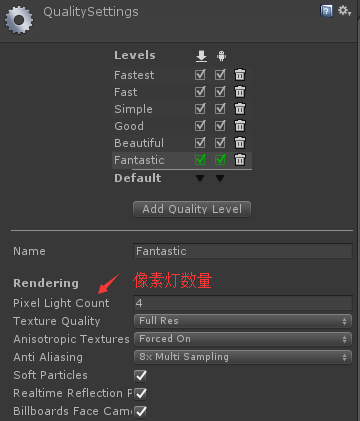
\includegraphics[width=.9\linewidth]{./pic/light.png}
\end{center}
\subsection{碰撞器}
\label{sec:org859ef02}
\begin{itemize}
\item (1)通常,碰撞器根据复杂度排序,对象越复杂,使用这个对象的性能开销越大。有可能的话,用盒子或者球体(Box/Sphere)来封装对象,这样碰撞器的计算最少。不要用网格碰撞器(Mesh Collider)。
\item (2)注意碰撞体的碰撞层,不必要的碰撞检测请舍去。
\end{itemize}
\subsection{贴图纹理}
\label{sec:org0911d23}
\begin{itemize}
\item (1)可以把图像纹理或者其它资源共享使用,尽量避免透明,可以使用填充黑色
\item (2)尝试用压缩贴图格式,或用16位代替32位。图片压缩将降低你的图片大小(更快地加载更小的内存跨度(footprint)),而且大大提高渲染表现。压缩贴图比起未压缩的32位RGBA贴图占用内存带宽少得多。
\item (3)之前U3D会议还听说过一个优化,贴图尽量都用一个大小的格式(512 * 512 , 1024 * 1024),这样在内存之中能得到更好的排序,而不会有内存之间空隙。
\item (4)MIPMAPs,跟网页上的略缩图原理一样,在3D游戏中我们为游戏的贴图生成多重纹理贴图,远处显示较小的物体用小的贴图,显示比较大的物体用精细的贴图。这样能更加有效的减少传输给GPU中的数据。但同时也会增加内存的大小,自己根据项目来权衡利弊
\item (5)如果你做了一个图集是1024X1024的。此时你的界面上只用了图集中的一张很小的图,那么很抱歉1024X1024这张大图都需要载入你的内存里面,1024就是4M的内存,如果你做了10个1024的图集,你的界面上刚好都只用了每个图集里面的一张小图,那么再次抱歉你的内存直接飙40M。意思是任何一个4096的图片,不管是图集还是texture,他都占用4*4=16M?
\item (6)IOS平台使用PVRTC压缩纹理。Adroid平台使用ETC1格式压缩。均可以减至1/4的内存大小,优化非常明显!目前主流的Android机型基本都支持ETC1格式压缩。但ETC1只能支持非Alpha通道的图片压缩。所以一般把Alpha通道图分离出来,绘制到GPU显存时,a值从Alpha图里获取,无Alpha通道的图就可以使用ETC1压缩。
\item (7)设置不透明贴图的压缩格式为ETC 4bit,因为android市场的手机中的GPU有多种,每家的GPU支持不同的压缩格式,但他们都兼容ETC格式
\begin{itemize}
\item 对于透明贴图,我们只能选择RGBA 16bit 或者RGBA 32bit。
\end{itemize}
\item (8)减少FPS,在 ProjectSetting -> Quality中的VSync Count 参数会影响你的FPS,EveryVBlank相当于FPS=60,EverySecondVBlank = 30;
\begin{itemize}
\item 如果这两种情况都不符合游戏的FPS的话,我们需要手动调整FPS,首先关闭垂直同步(VSync = Vertical Sync)这个功能,即设置VSync为Don't Sync
\item 然后在代码的Awake方法里手动设置FPS
\end{itemize}
\begin{minted}[linenos=true]{java}
Application.targetFrameRate = 45;
\end{minted}
\begin{itemize}
\item 降低FPS的好处:
\begin{itemize}
\item 1)省电,减少手机发热的情况;
\item 2)能都稳定游戏FPS,减少出现卡顿的情况。
\end{itemize}
\end{itemize}
\item (9)当我们设置了FPS后,再调整下Fixed timestep这个参数,这个参数在ProjectSetting->Time中,目的是减少物理计算的次数,来提高游戏性能。
\item (10)尽量少使用Update LateUpdate FixedUpdate,这样也可以提升性能和节省电量。多使用事件(不是SendMessage,使用自己写的,或者C\#中的事件委托)。
\item (11)待机时,调整游戏的FPS为1,节省电量。
\item (12)图集大小最好不要高于1024,否则游戏安装之后、低端机直接崩溃、原因是手机系统版本低于2.2、超过1000的图集无法读取导致。2.2 以上没有遇见这个情况。注意手机的RAM 与 ROM、小于 512M的手机、直接放弃机型适配。
\item (13)不同设备要使用不同的纹理大小,尤其是UI和大型背景中的纹理。《Shadow Blade》使用的是通用型模板,但如果在启动时检测到设备大小和分辨率,就会载入不同资产。
\item (14)远处的物体绘制在skybox上
\end{itemize}
\subsection{脚本}
\label{sec:orgee5b234}
\begin{itemize}
\item (1)如果你不需要运行某一个脚本,那么就禁用它。不管它多少的小,或者出现的很少,但每一个处理都需要占用时间。
\item (2)不要留着未实现的Update,FixedUpdate等方法,用不到就删除,不然会执行,消耗时间!
\item (3)移除代码中的任何字符串连接,因为这会给GC留下大量垃圾。使用StringBuilder链接字符串
\item (4)用简单的"for"循环代替"foreach"循环。由于某些原因,每个"foreach"循环的每次迭代会生成24字节的垃圾内存。一个简单的循环迭代10次就可以留下240字节的垃圾内存。
\item (5)更改我们检查游戏对象标签的方法。用 "if (go.CompareTag ("Enemy")"来代替"if (go.tag == "Enemy")" 。

\begin{minted}[linenos=true]{java}
  if (go.CompareTag ("Enemy")) {}
  // 来代替
  // if (go.tag == "Enemy")
\end{minted}
\begin{itemize}
\item 在一个内部循环调用对象分配的标签属性以及拷贝额外内存,这是一个非常糟糕的做法。
\end{itemize}
\item (6)不使用LINQ命令,因为它们一般会分配中间缓器,而这很容易生成垃圾内存。
\item (7)修改代码以免依赖"ControllerColliderHit" 回调函数。这证明这些回调函数处理得并不十分迅速。
\item (8)要谨慎评估触发器的"onInside"回调函数,在我们的项目中,我们尽量在不依赖它们的情况下模拟逻辑。
\item (9)注意是否有多余的动画脚本,模型自动导入到U3D会有动画脚本,大量的话会严重影响消耗CPU计算。
\item (10)尽量避免每帧处理,可以每隔几帧处理一次 
\begin{minted}[linenos=true]{java}
void Update() { 
    if (Time.frameCount % 5 == 0) { 
        DoSomeThing(); 
    } 
}
\end{minted}
\item (11)尽量避免使用float,而使用int,特别是在手机游戏中,尽量少用复杂的数学函数,比如sin,cos等函数。改除法/为乘法,例如:使用x*0.5f而不是 x/2.0f 。
\item (12)避免使用
\begin{minted}[linenos=true]{java}
for (int i = 0; i < myArray.Length; i++)
\end{minted}
\begin{itemize}
\item 而应该这样
\end{itemize}
\begin{minted}[linenos=true]{java}
int length = myArray.Length;  
for (int i = 0; i < length; i++)  
\end{minted}
\item (13)少使用临时变量,特别是在Update OnGUI等实时调用的函数中定义临时变量。
\item (14)协同是一个好方法。可以使用协同程序来代替不必每帧都执行的方法。(还有InvokeRepeating方法也是一个好的取代Update的方法)。
\item (15)不要使用SendMessage之类的方法,他比直接调用方法慢了100倍,你可以直接调用或通过C\#的委托来实现。
\item (16)操作transform.localPosition的时候请小心,移动GameObject是非常平常的一件事情,以下代码看起来很简单:  
\begin{minted}[linenos=true]{java}
     transform.localPosition += new Vector3 ( 10.0f * Time.deltaTime, 0.0f, 0.0f );
\end{minted}
\begin{itemize}
\item 但是小心了,假设上面这个GameObject有一个parent, 并且这个parent GameObject的localScale是(2.0f, 2.0f, 2.0f)。你的GameObject将会移动20.0个单位/秒。
\item 因为该 GameObject的world position等于:
\end{itemize}

\begin{minted}[linenos=true]{java}
Vector3 offset = new Vector3( my.localPosition.x * parent.lossyScale.x, 
                              my.localPosition.y * parent.lossyScale.y, 
                              my.localPosition.z * parent.lossyScale.z );
Vector3 worldPosition = parent.position + parent.rotation * offset;
\end{minted}
\begin{itemize}
\item 换句话说,上面这种直接操作localPosition的方式是在没有考虑scale计算的时候进行的,为了解决这个问题,unity3d提供了Translate函数, 所以正确的做法应该是:
\end{itemize}
\begin{minted}[linenos=true]{java}
transform.Translate ( 10.0f * Time.deltaTime, 0.0f, 0.0f );
\end{minted}
\item (17)减少固定增量时间, 将固定增量时间值设定在0.04-0.067区间(即,每秒15-25帧)。您可以通过Edit -> Project Settings -> Time来改变这个值。这样做降低了FixedUpdate函数被调用的频率以及物理引擎执行碰撞检测与刚 体更新的频率。如果您使用了较低的固定增量时间,并且在主角身上使用了刚体部件,那么您可以启用插值办法来平滑刚体组件。
\item (18)减少GetComponent的调用使用,GetComponent或内置组件访问器(transform)会产生明显的开销。您可以通过一次获取组件的引用来避免开销,并将该引用分配给一个变量(有时称为"缓存"的引用)。
\begin{minted}[linenos=true]{java}
Transform myTransform ;
void Awake () {
    myTransform = transform;
}
\end{minted}
\item (19)同时,在某些可能的情况下,您也可以使用结构(struct)来代替类(class)。这是因为,结构变量主要存放在栈区而非堆区。因为栈的分配较快,并且不调用垃圾回收操作,所以当结构变量比较小时可以提升程序的运行性能。但是当结构体较大时,虽然它仍可避免分配/回收的开销,而它由于"传值"操作也会导致单独的开销,实际上它可能比等效对象类的效率还要低。
\item (20)使用GUILayout 函数可以很方便地将GUI元素进行自动布局。然而,这种自动化自然也附带着一定的处理开销。您可以通过手动的GUI功能布局来避免这种开销。此外,您也可以设置一个脚本的useGUILayout变量为 false来完全禁用GUI布局:
\end{itemize}
\begin{minted}[linenos=true]{java}
void Awake () {
   useGUILayout = false;
}
\end{minted}
\begin{itemize}
\item (21)最小化碰撞检测请求(例如ray casts和sphere checks),尽量从每次检查中获得更多信息。
\item (22)在edit->project setting->time中调大FixedTimestep(真实物理的帧率)来减少cpu损耗
\item (23)尽量不要动态的instantiate和destroy object,使用object pool
\item (24)尽量不要再update函数中做复杂计算,如有需要,可以隔N帧计算一次
\item (25)不要使用内置的onGUii函数处理gui,使用其他方案,如NGUI
\end{itemize}
\subsection{组件}
\label{sec:orgb42a9dc}
\begin{itemize}
\item (1)尽可能的使用简单组件—如果你不需求功能较多的组件,那么就自己去实现它避免一起使用大量系统组件。比如,CharacterController是一个很废资源的组件,那么最好使用刚体来定义自己的解决方案。
\item (2)面对性能更弱的设备,要用skinned mesh代替physics cloth。cloth参数在运行表现中发挥重要作用,如果你肯花些时间找到美学与运行表现之间的平衡点,就可以获得理想的结果。
\item (3)在物理模拟过程中不要使用ragdolls( 布娃娃系统),只有在必要时才让它生效。
\item (4)真实的物理(刚体)很消耗,不要轻易使用,尽量使用自己的代码模仿假的物理
\end{itemize}
\subsection{NGUI}
\label{sec:org77c7aa5}
\begin{itemize}
\item (1)NGUI中所有Panel都有一个Depth值影响着他下面的所有挂件。如果你正在创建一个使用多个窗口的复杂UI,通常最好的做法是每个窗口有一个UIPanel。请确认你的panel不会拥有相同的depth值。如果这个值是一样的,为了保证绘制顺序,draw call将会开始频繁分割,这将导致产生比平常更多的draw call。
\end{itemize}
\subsection{顶点数}
\label{sec:orga6e4d55}
\begin{itemize}
\item (1)尽量减少顶点数
\end{itemize}
\subsection{材质}
\label{sec:org7c0f710}
\begin{itemize}
\item (1)尽可能共用材质。这样便可以减少DrawCall,引擎可以进行其批处理!
\item (2)如果你需要通过脚本来控制单个材质属性,需要注意改变Renderer.material将会造成一份材质的拷贝。因此,你应该使用Renderer.sharedMaterial来保证材质的共享状态。
\item (3)有一个合并模型材质不错的插件叫Mesh Baker
\end{itemize}
\subsection{特效}
\label{sec:org4044ae9}
\begin{itemize}
\item (1)如果不需要别用雾效(fog)
\item (2)要找到美学/性能之间的平衡,就免不了许多粒子效果的迭代。减少发射器数量并尽量减少透明度需求也是一大挑战。
\end{itemize}
\subsection{模型物体}
\label{sec:org1bcb529}
\begin{itemize}
\item (1)不要有不必要的三角面。面片数最好控制在300\textasciitilde{}2000面片
\item (2)UV贴图中的接缝和硬边越少越好。
\begin{itemize}
\item 需要注意的是,图形硬件需要处理顶点数和硬件报告说的并不一样。不是硬件说能渲染几个点就是几个点。模型处理应用通常展示的是几何顶点数量。例如,一个由一些不同顶点构成的模型。在显卡中,一些集合顶点将会被分离(split)成两个或者更多逻辑顶点用作渲染。如果有法线、UV坐标、顶点色的话,这个顶点必须会被分离。所以在游戏中处理的实际数量显然要多很多。
\end{itemize}
\item (3)LOD (Level Of Detail) 是很常用的3D游戏技术了,其功能理解起来则是相当于多重纹理贴图。在以在屏幕中显示模型大小的比例来判断使用高或低层次的模型来减少对GPU的传输数据,和减少GPU所需要的顶点计算。
\item (4)摄像机分层距离剔除(Per-Layer Cull Distances):为小物体标识层次,然后根据其距离主摄像机的距离判断是否需要显示。
\item (5)遮挡剔除(Occlusion Culling)其实就是当某个物体在摄像机前被另外一个物体完全挡住的情况,挡住就不发送给GPU渲染,从而直接降低DRAW CALL。不过有些时候在CPU中计算其是否被挡住则会很耗计算,反而得不偿失。
\item (6)将不需要移动的物体设为Static,让引擎可以进行其批处理。
\item (7)用单个蒙皮渲染、尽量少用材质、少用骨骼节点、移动设备上角色多边形保持在300\textasciitilde{}1500内(当然还要看具体的需求)、PC平台上1500\textasciitilde{}4000内(当然还要看具体的需求)。
\begin{itemize}
\item 角色的面数一般不要超过1500,骨骼数量少于30就好,越多的骨骼就会越多的带来CPU消耗,角色Material数量一般1\textasciitilde{}2个为最佳。
\end{itemize}
\item (8)导入 3D 模型之后,在不影响显示效果的前提下,最好打开 Mesh Compression。Off, Low, Medium, High 这几个选项,可酌情选取。
\item (9)避免大量使用unity自带的 Sphere 等内建 Mesh,Unity 内建的 Mesh,多边形的数量比较大,如果物体不要求特别圆滑,可导入其他的简单3D模型代替。
\item (10)每个角色尽量使用一个Skinned Mesh Renderer,这是因为当角色仅有一个 Skinned Mesh Renderer 时,Unity 会使用视锥型可见性裁剪和多边形网格包围体更新的方法来优化角色的运动,而这种优化只有在角色仅含有一个 Skinned Mesh Renderer时才会启动。
\item (11)对于静态物体顶点数要求少于500,UV的取值范围不要超过(0,1)区间,这对于纹理的拼合优化很有帮助。
\item (12)不需要的Animation组件就删掉
\end{itemize}
\subsection{粒子系统}
\label{sec:orgffdf3e6}
\begin{itemize}
\item 粒子系统运行在iPhone上时很慢,怎么办?因为iPhone拥有相对较低的fillrate 。如果您的粒子效果覆盖大部分的屏幕,而且是multiple layers的,这样即使最简单的shader,也能让iPhone傻眼。我们建议把您的粒子效果baking成纹理序列图。然后在运行时可以使用1-2个粒子,通过动画纹理来显示它们。这种方式可以取得很好的效果,以最小的代价。
\item 自带地形:地形高度图尺寸小于257,尽量使用少的混合纹理数目,尽量不要超过4个,Unity自带的地形时十分占资源的,强烈建议不要使用,自己制作地形,尽量一张贴图搞定
\begin{itemize}
\item drawcall是啥?draw:绘制,call:调用,其实就是对底层图形程序(比如:OpenGL ES)接口的调用,以在屏幕上画出东西。那么,是谁去调用这些接口呢?CPU。
\item fragment是啥?经常有人说vf啥的,vertex我们都知道是顶点,那fragment是啥呢?说它之前需要先说一下像素,像素各位应该都知道吧?像素是构成数码影像的基本单元呀。那fragment呢?是有可能成为像素的东西。啥叫有可能?就是最终会不会被画出来不一定,是潜在的像素。这会涉及到谁呢?GPU。
\item batching是啥?都知道批处理是干嘛的吧?没错,将批处理之前需要很多次调用(drawcall)的物体合并,之后只需要调用一次底层图形程序的接口就行。听上去这简直就是优化的终极方案啊!但是,理想是美好的,世界是残酷的,一些不足之后我们再细聊。
\item 内存的分配:记住,除了Unity3D自己的内存损耗。我们可是还带着Mono呢啊,还有托管的那一套东西呢。更别说你一激动,又引入了自己的几个dll。这些都是内存开销上需要考虑到的。
\item CPU方面: 
\begin{itemize}
\item 上文中说了,drawcall影响的是CPU的效率,而且也是最知名的一个优化点。但是除了drawcall之外,还有哪些因素也会影响到CPU的效率呢?让我们一一列出暂时能想得到的:
\begin{itemize}
\item (1)DrawCalls
\item (2)物理组件(Physics)
\item (3)GC(什么?GC不是处理内存问题的嘛?匹夫你不要骗我啊!不过,匹夫也要提醒一句,GC是用来处理内存的,但是是谁使用GC去处理内存的呢?)
\item (4)当然,还有代码质量
\end{itemize}
\end{itemize}
\end{itemize}
\end{itemize}
\subsection{DrawCalls:}
\label{sec:orgb31cbd5}
\begin{itemize}
\item 前面说过了,DrawCall是CPU调用底层图形接口。比如有上千个物体,每一个的渲染都需要去调用一次底层接口,而每一次的调用CPU都需要做很多工作,那么CPU必然不堪重负。但是对于GPU来说,图形处理的工作量是一样的。所以对DrawCall的优化,主要就是为了尽量解放CPU在调用图形接口上的开销。所以针对drawcall我们主要的思路就是每个物体尽量减少渲染次数,多个物体最好一起渲染。所以,按照这个思路就有了以下几个方案:
\begin{itemize}
\item 使用Draw Call Batching,也就是描绘调用批处理。Unity在运行时可以将一些物体进行合并,从而用一个描绘调用来渲染他们。具体下面会介绍。
\item 通过把纹理打包成图集来尽量减少材质的使用。
\item 尽量少的使用反光啦,阴影啦之类的,因为那会使物体多次渲染。
\end{itemize}
\end{itemize}
\subsection{Draw Call Batching}
\label{sec:orge56cb96}
\begin{itemize}
\item 首先我们要先理解为何2个没有使用相同材质的物体即使使用批处理,也无法实现Draw Call数量的下降和性能上的提升。
\item 因为被"批处理"的2个物体的网格模型需要使用相同材质的目的,在于其纹理是相同的,这样才可以实现同时渲染的目的。因而保证材质相同,是为了保证被渲染的纹理相同。
\item 因此,为了将2个纹理不同的材质合二为一,我们就需要进行上面列出的第二步,将纹理打包成图集。具体到合二为一这种情况,就是将2个纹理合成一个纹理。这样我们就可以只用一个材质来代替之前的2个材质了。
\item 而Draw Call Batching本身,也还会细分为2种。
\end{itemize}
\subsection{Static Batching 静态批处理}
\label{sec:org2f0c3f2}
\begin{itemize}
\item 看名字,猜使用的情景。
\item 静态?那就是不动的咯。还有呢?额,听上去状态也不会改变,没有"生命",比如山山石石,楼房校舍啥的。那和什么比较类似呢?嗯,聪明的各位一定觉得和场景的属性很像吧!所以我们的场景似乎就可以采用这种方式来减少draw call了。
\item 那么写个定义:只要这些物体不移动,并且拥有相同的材质,静态批处理就允许引擎对任意大小的几何物体进行批处理操作来降低描绘调用。
\item 那要如何使用静态批来减少Draw Call呢?你只需要明确指出哪些物体是静止的,并且在游戏中永远不会移动、旋转和缩放。想完成这一步,你只需要在检测器(Inspector)中将Static复选框打勾即可!
\item 至于效果如何呢?
\item 举个例子:新建4个物体,分别是Cube,Sphere, Capsule, Cylinder,它们有不同的网格模型,但是也有相同的材质(Default-Diffuse)。
\item 首先,我们不指定它们是static的。Draw Call的次数是4次,如图:
\end{itemize}

\begin{center}
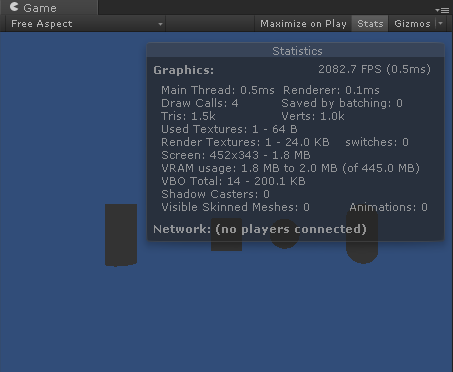
\includegraphics[width=.9\linewidth]{./pic/batching1.png}
\end{center}
\begin{itemize}
\item 我们现在将它们4个物体都设为static,在来运行一下:
\end{itemize}

\begin{center}
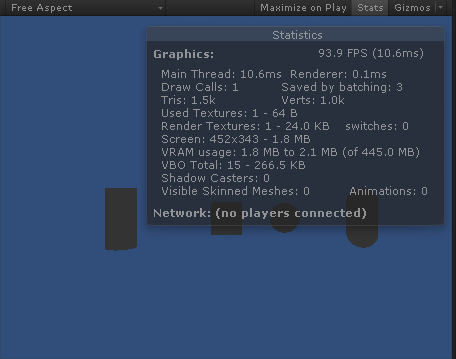
\includegraphics[width=.9\linewidth]{./pic/batching2.png}
\end{center}
\begin{itemize}
\item 如图,Draw Call的次数变成了1,而Saved by batching的次数变成了3。
\item 静态批处理的好处很多,其中之一就是与下面要说的动态批处理相比,约束要少很多。所以一般推荐的是draw call的静态批处理来减少draw call的次数。那么接下来,我们就继续聊聊draw call的动态批处理。
\end{itemize}
\subsection{Dynamic Batching 动态批处理}
\label{sec:org806bd41}
\begin{itemize}
\item 有阴就有阳,有静就有动,所以聊完了静态批处理,肯定跟着就要说说动态批处理了。首先要明确一点,Unity3D的draw call动态批处理机制是引擎自动进行的,无需像静态批处理那样手动设置static。我们举一个动态实例化prefab的例子,如果动态物体共享相同的材质,则引擎会自动对draw call优化,也就是使用批处理。首先,我们将一个cube做成prefab,然后再实例化50次,看看draw call的数量。
\end{itemize}
\begin{minted}[linenos=true]{java}
for (int i = 0; i < 50; i++) {
    GameObject cube;
    cube = GameObject.Instantiate(prefab) as GameObject;
}
\end{minted}
\begin{itemize}
\item draw call的数量:

\begin{center}
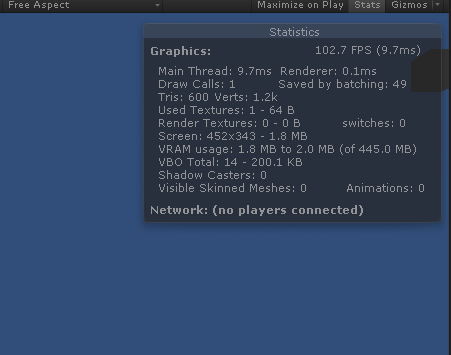
\includegraphics[width=.9\linewidth]{./pic/drawcall.png}
\end{center}
\item 可以看到draw call的数量为1,而 saved by batching的数量是49。而这个过程中,我们除了实例化创建物体之外什么都没做。不错,unity3d引擎为我们自动处理了这种情况。
\item 但是有很多童靴也遇到这种情况,就是我也是从prefab实例化创建的物体,为何我的draw call依然很高呢?这就是匹夫上文说的,draw call的动态批处理存在着很多约束。下面匹夫就演示一下,针对cube这样一个简单的物体的创建,如果稍有不慎就会造成draw call飞涨的情况吧。
\item 我们同样是创建50个物体,不同的是其中的10个物体,每个物体的大小都不同,也就是Scale不同。
\end{itemize}
\begin{minted}[linenos=true]{java}
for (int i = 0; i < 50; i++) {
    GameObject cube;
    cube = GameObject.Instantiate(prefab) as GameObject;
    if (i / 10 == 0) {
        cube.transform.localScale = new Vector3(2 + i, 2 + i, 2 + i);
    }
}
\end{minted}

\begin{center}
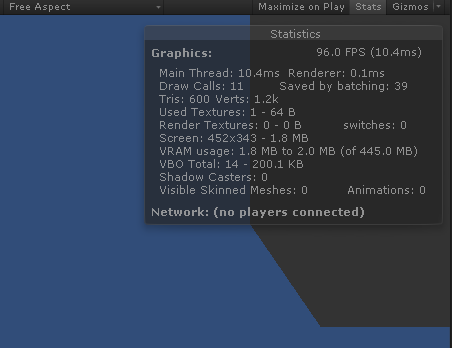
\includegraphics[width=.9\linewidth]{./pic/drawcall2.png}
\end{center}
\section{Unity UI/GUI/UGUI/NGUI}
\label{sec:org8dfef2a}
\subsection{Unity3D快速实现UI架构设计一}
\label{sec:org0395e8e}
\begin{itemize}
\item \url{https://blog.csdn.net/jxw167/article/details/72057771}
\end{itemize}

\subsection{NGUI与UGUI最详细对比}
\label{sec:orgaa0d517}
\begin{itemize}
\item \url{http://www.u3dc.com/archives/412}
\item 1.ugui的ui根目录为canvas(画布),ngui则是uiroot。在命名上官方似乎更贴合想象力。
\item 2.在屏幕自适应方面,ugui为render mode。ngui则为scaling style。
\item 3.anchor(锚点)的使用方式差不多,都是用来固定位置,在可视化方面,ugui的花瓣锚点真不太好调。
\item 4.ngui灵活性不是一般的高,随意创建一个sprite,加了boxcollider,它就可以是按钮、滑动条……
\item 5.ugui的sprite的切图功能真心不错。ngui使用图集不能直接拖拉(毕竟是三方插件)略不方便。
\item 6.ngui的tween动画功能很省心,无需额外定义代码,使用封装好的脚本就可以实现一些简单动画,叠加脚本甚至能实现相对复杂的动画效果。
\item 最后,强大的网友分享了一张比较全面的对比图(点击图片放大):
\item \begin{center}
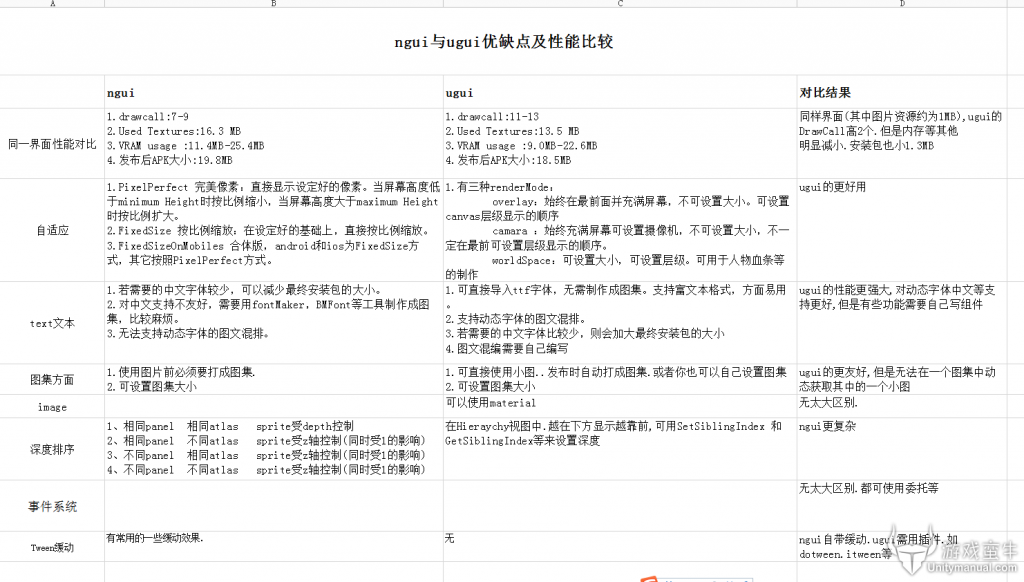
\includegraphics[width=.9\linewidth]{./pic/ngui-ugui.png}
\end{center}
\end{itemize}
\subsection{关于Unity中的UGUI优化,你可能遇到这些问题}
\label{sec:org750f515}
\begin{itemize}
\item \url{https://blog.uwa4d.com/archives/QA\_UGUI-1.html}
\end{itemize}
\subsubsection{界面制作}
\label{sec:orgaf3e46f}
\begin{enumerate}
\item UGUI里的这个选项 ,应该是ETC2拆分Alpha通道的意思,但是在使用中并没起作用?请问有没有什么拆分的标准和特别要求呢?
\label{sec:org507a082}

\begin{center}
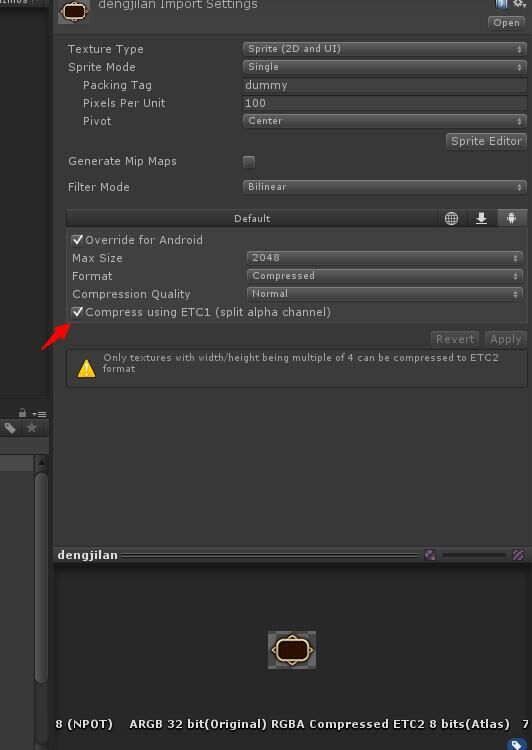
\includegraphics[width=.9\linewidth]{./pic/ugui1.jpg}
\end{center}
\begin{itemize}
\item 据我们所知,alpha split 的功能最初只对 Unity 2D 的 Sprite(SpriteRenderer)有完整的支持,而UI的支持是在Unity 5.4版本之后的。建议大家在Unity 5.4版本以后的UGUI中尝试该功能。
\end{itemize}
\item 在UI界面中,用Canvas还是用RectTransform做根节点更好?哪种方法效率更高?
\label{sec:orgc68317b}
\begin{itemize}
\item Canvas划分是个很大的话题。简单来说,因为一个Canvas下的所有UI元素都是合在一个Mesh中的,过大的Mesh在更新时开销很大,所以一般建议每个较复杂的UI界面,都自成一个Canvas(可以是子Canvas),在UI界面很复杂时,甚至要划分更多的子Canvas。同时还要注意动态元素和静态元素的分离,因为动态元素会导致Canvas的mesh的更新。最后,Canvas又不能细分的太多,因为会导致Draw Call的上升。我们后续将对UI模块做具体的讲解,尽请期待。
\end{itemize}
\item UWA性能检测报告中的Shared UI Mesh表示什么呢?
\label{sec:orgc4ee66e}

\begin{center}
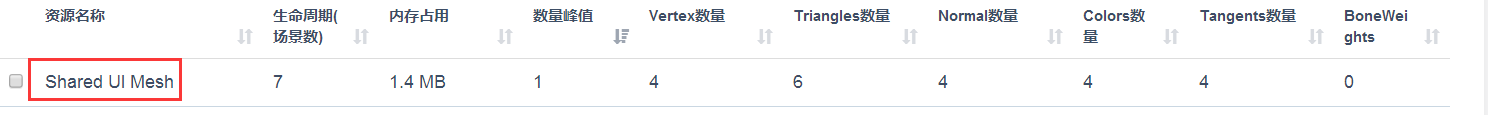
\includegraphics[width=.9\linewidth]{./pic/ugui2.jpg}
\end{center}
\begin{itemize}
\item Shared UI Mesh是在Unity 5.2 版本后UGUI系统维护的UI Mesh。在以前的版本中,UGUI会为每一个Canvas维护一个Mesh(名为BatchedMesh,其中再按材质分为不同的SubMesh)。而在Unity 5.2版本后,UGUI底层引入了多线程机制,而其Mesh的维护也发生了改变,目前Shared UI Mesh作为静态全局变量,由底层直接维护,其大小与当前场景中所有激活的UI元素所生成的网格数相关。
\item 一般来说当界面上UI元素较多,或者文字较多时该值都会较高,在使用UI/Effect/shadow和UI/Effect/Outline时需要注意该值,因为这两个Effect会明显增加文字所带来的网格数。
\end{itemize}
\item 在使用NGUI时,我们通常会将很多小图打成一个大的图集,以优化内存和Draw Call。而在UGUI时代,UI所使用的Image必须是Sprite;Unity提供了SpritePacker。 它的工作流程和UGUI Atlas Paker有较大的差别。在Unity Asset中,我们压根看不到图集的存在。 问题是:
\label{sec:orgeb9c0c1}
\begin{itemize}
\item 1. SpritePacker大概的工作机制是什么样的?
\item 2. 如果Sprite没有打包成AssetBundle,直接在GameObject上引用,那么在Build时Unity会将分散的Sprite拼接在一起么?如果没有拼接,那SpritePacker是不是只会优化Draw Call,内存占用上和不用SpritePacker的分离图效果一样?
\item 3. 如果将Sprite打成AssetBundle,AssetBundle中的资源是分散的Sprite吗?如果不是,不同的AssetBundle中引用了两张Sprite,这两张Sprite恰好用SpritePacker拼在了一起,是不是就会存在两份拼接的Sprite集?
\item 4. 如果想使用NGUI Atlas Packer的工作流程,该如何去实现?
\begin{itemize}
\item 简单来说,UGUI和 NGUI 类似,但是更加自动化。只需要通过设定 Packing Tag 即可指定哪些 Sprite 放在同一个 Atlas 下。
\begin{itemize}
\item 可以通过 Edit -> Project Settings -> Editor -> Sprite Packer 的 Mode 来设置是否起效,何时起效(一种是进入 Play Mode 就生效,一种是 Build 时才生效)。所以只要不选 Disabled,Build 时就会把分散的 Sprite 拼起来。
\item 可以认为 Sprite 就是一个壳子,实际上本身不包含纹理资源,所以打包的时候会把Atlas 打进去。如果不用依赖打包,那么分开打两个 Sprite 就意味各自的AssetBundle 里都会有一个 Atlas。
\item 可以通过第三方工具(如 Texture Packer)制作 Atlas,导出 Sprite 信息(如,第 N 个 Sprite 的 Offset 和 Width,Height 等),然后在 Unity 中通过脚本将该 Atlas 转成一个 Multiple Mode 的 Sprite 纹理(即一张纹理上包含了多个 Sprite),同时禁用 Unity 的 Sprite Packer 即可。
\end{itemize}
\item 两种做法各有利弊,建议分析一下两种做法对于自身项目的合适程度来进行选择。
\end{itemize}
\end{itemize}
\item 在Unity 5.x版本下,我们在用UGUI的过程中发现它把图集都打进了包里,这样就不能自动更新了,请问图集怎么做自动更新呢?
\label{sec:orgc272ac4}
\begin{itemize}
\item 在Unity 5.x中UGUI使用的Atlas确实是不可见的,因此无法直接将其独立打包。但我们建议,可以把Packing Tag相同的源纹理文件,打到同一个AssetBundle中(设置一样的AssetBundle Name),从而避免Atlas的冗余。同时这样打包可以让依赖它的Canvas的打包更加自由,即不需要把依赖它的Canvas都打在一个AssetBundle中,在更新时直接更新Atlas所在的AssetBundle即可。
\end{itemize}
\item ScrollRect在滚动的时候,会产生Canvas.SendwillRenderCanvases,有办法消除吗?
\label{sec:org219354d}
\begin{itemize}
\item ScrollRect在滚动时,会产生OnTransformChanged的开销,这是UI元素在移动时触发的,但通常这不会触发Canvas.SendWillRenderCanvases。
\item 如果观察到Canvas.SendWillRenderCanvases耗时较高,可以检查下ScrollRect所在的Canvas是否开启了Pixel Perfect的选项,该选项的开启会导致UI元素在发生位移时,其长宽会被进行微调(为了对其像素),而ScrollRect中通常有较多的UI元素,从而产生较高的Canvas.SendWillRenderCanvases开销。因此可以尝试关闭Pixel Perfect看效果是否可以接受,或者尝试在滚动过程中暂时关闭Pixel Perfect等方式来消除其开销。
\end{itemize}
\end{enumerate}
\subsubsection{网格重建}
\label{sec:orgc0567e4}
\begin{enumerate}
\item 我在UGUI里更改了Image的Color属性,那么Canvas是否会重建?我只想借用它的Color做Animation里的变化量。
\label{sec:orga0acb41}
\begin{itemize}
\item 如果修改的是Image组件上的Color属性,其原理是修改顶点色,因此是会引起网格的Rebuild的(即Canvas.BuildBatch操作,同时也会有Canvas.SendWillRenderCanvases的开销)。而通过修改顶点色来实现UI元素变色的好处在于,修改顶点色可以保证其材质不变,因此不会产生额外的Draw Call。
\end{itemize}
\item Unity自带的UI Shader处理颜色时,改\textsubscript{Color属性不会触发顶点重建吗}?
\label{sec:org6ffc6cf}
\begin{itemize}
\item 在UI的默认Shader中存在一个Tint Color的变量,正常情况下,该值为常数(1,1,1),且并不会被修改。如果是用脚本访问Image的Material,并修改其上的Tint Color属性时,对UI元素产生的网格信息并没有影响,因此就不会引起网格的Rebuild。但这样做因为修改了材质,所以会增加一个Draw Call。
\end{itemize}
\item 能否就UGUI Batch提出一些建议呢?是否有一些Batch的规则?
\label{sec:org62838d4}
\begin{itemize}
\item 在 UGUI 中,Batch是以Canvas为单位的,即在同一个Canvas下的UI元素最终都会被Batch到同一个Mesh中。而在Batch前,UGUI会根据这些UI元素的材质(通常就是Atlas)以及渲染顺序进行重排,在不改变渲染结果的前提下,尽可能将相同材质的UI元素合并在同一个SubMesh中,从而把DrawCall降到最低。而Batch的操作只会在UI元素发生变化时才进行,且合成的Mesh越大,操作的耗时也就越大。
\item 因此,我们建议尽可能把频繁变化(位置,颜色,长宽等)的UI元素从复杂的Canvas中分离出来,从而避免复杂的Canvas频繁重建。
\end{itemize}
\item 我用的是UGUI Canvas,Unity 5.3.4版本,请问如何查看每次Rebuild Batch影响的顶点数, Memory Profiler是个办法但是不好定位。
\label{sec:org245b40d}
\begin{itemize}
\item 由于Unity引擎在5.2后开始使用Shared UI Mesh来存储UI Mesh,所以确实很难查看每次Rebuild的UI顶点数。但是,研发团队可以尝试通过Frame Debugger工具对UI界面进行进一步的查看。
\end{itemize}
\item 动静分离或者多Canvas带来性能提升的理论基础是什么呢?如果静态部分不变动,整个Canvas就不刷新了?
\label{sec:orgc1ee292}
\begin{itemize}
\item 在UGUI中,网格的更新或重建(为了尽可能合并UI部分的DrawCall)是以Canvas为单位的,且只在其中的UI元素发生变动(位置、颜色等)时才会进行。因此,将动态UI元素与静态UI元素分离后,可以将动态UI元素的变化所引起的网格更新或重建所涉及到的范围变小,从而降低一定的开销。而静态UI元素所在的Canvas则不会出现网格更新和重建的开销。
\end{itemize}
\item UWA建议“尽可能将静态UI元素和频繁变化的动态UI元素分开,存放于不同的Panel下。同时,对于不同频率的动态元素也建议存放于不同的Panel中。”那么请问,如果把特效放在Panel里面,需要把特效拆到动态的里面吗?
\label{sec:org53f83ec}
\begin{itemize}
\item 通常特效是指粒子系统,而粒子系统的渲染和UI是独立的,仅能通过Render Order来改变两者的渲染顺序,而粒子系统的变化并不会引起UI部分的重建,因此特效的放置并没有特殊的要求。
\end{itemize}
\item 多人同屏的时候,人物移动会使得头顶上的名字Mesh重组,从而导致较为严重的卡顿,请问一下是否有优化的办法?
\label{sec:orgce6ea85}
\begin{itemize}
\item 如果是用UGUI开发的,当头顶文字数量较多时,确实很容易引起性能问题,可以考虑从以下几点入手进行优化:
\begin{itemize}
\item 尽可能避免使用UI/Effect,特别是Outline,会使得文本的Mesh增加4倍,导致UI重建开销明显增大;
\item 拆分Canvas,将屏幕中所有的头顶文字进行分组,放在不同的Canvas下,一方面可以降低更新的频率(如果分组中没有文字移动,该组就不会重建),另一方面可以减小重建时涉及到的Mesh大小(重建是以Canvas为单位进行的);
\item 降低移动中的文字的更新频率,可以考虑在文字移动的距离超过一个阈值时才真正进行位移,从而可以从概率上降低Canvas更新的频率。
\end{itemize}
\end{itemize}
\end{enumerate}
\subsubsection{界面切换}
\label{sec:orgbc84a24}
\begin{enumerate}
\item 游戏中出现UI界面重叠,该怎么处理较好?比如当前有一个全屏显示的UI界面,点其中一个按钮会再起一个全屏界面,并把第一个UI界面盖住。我现在的做法是把被覆盖的界面 SetActive(False),但发现后续 SetActive(True) 的时候会有 GC.Alloc 产生。这种情况下,希望既降低 Batches 又降低 GC Alloc 的话,有什么推荐的方案吗?
\label{sec:org54c16ee}
\begin{itemize}
\item 可以尝试通过添加一个 Layer 如 OutUI, 且在 Camera 的 Culling Mask 中将其取消勾选(即不渲染该 Layer)。从而在 UI 界面切换时,直接通过修改 Canvas 的 Layer 来实现“隐藏”。但需要注意事件的屏蔽,禁用动态的 UI 元素等等。
\item 这种做法的优点在于切换时基本没有开销,也不会产生多余的 Draw Call,但缺点在于“隐藏时”依然还会有一定的持续开销(通常不太大),而其对应的 Mesh 也会始终存在于内存中(通常也不太大)。
\item 以上的方式可供参考,而性能影响依旧是需要视具体情况而定。
\end{itemize}
\item 如图,我们在UI打开或者移动到某处的时候经常会观测到CPU上的冲激,经过进一步观察发现是因为Instantiate产生了大量的GC。想请问下Instantiate是否应该产生GC呢?我们能否通过资源制作上的调整来避免这样的GC呢?如下图,因为一次性产生若干MB的GC在直观感受上还是很可观的。
\label{sec:org20172f1}

\begin{center}
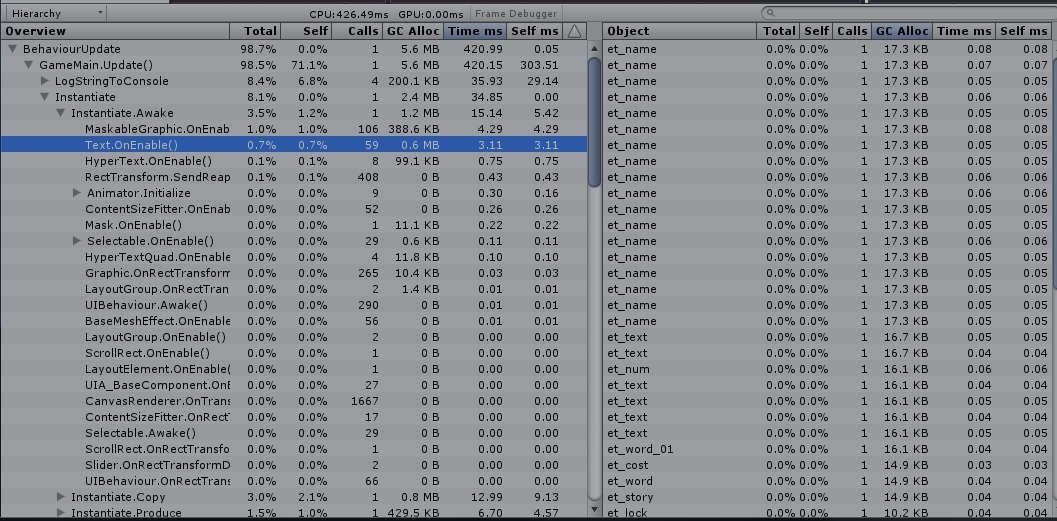
\includegraphics[width=.9\linewidth]{./pic/ugui3.jpg}
\end{center}
\begin{itemize}
\item 准确的说这些 GC Alloc 并不是由Instantiate 直接引起的,而是因为被实例化出来的组件会进行 OnEnable 操作,而在 OnEnable 操作中产生了 GC,比如以上图中的函数为例:
\item 上图中的 Text.OnEnable 是在实例化一个 UI 界面时,UI 中的文本(即 Text 组件)进行了 OnEnable 操作,其中主要是初始化文本网格的信息(每个文字所在的网格顶点,UV,顶点色等等属性),而这些信息都是储存在数组中(即堆内存中),所以文本越多,堆内存开销越大。但这是不可避免的,只能尽量减少出现次数。
\item 因此,我们不建议通过 Instantiate/Destroy 来处理切换频繁的 UI 界面,而是通过 SetActive(true/false),甚至是直接移动 UI 的方式,以避免反复地造成堆内存开销。
\end{itemize}
\end{enumerate}
\subsubsection{加载相关}
\label{sec:org812c5e6}
\begin{enumerate}
\item UGUI的图集操作中我们有这么一个问题,加载完一张图集后,使用这个方式获取其中一张图的信息:assetBundle.Load (subFile, typeof (Sprite)) as Sprite; 这样会复制出一个新贴图(图集中的子图),不知道有什么办法可以不用复制新的子图,而是直接使用图集资源 。
\label{sec:org4f0ee18}

\begin{center}
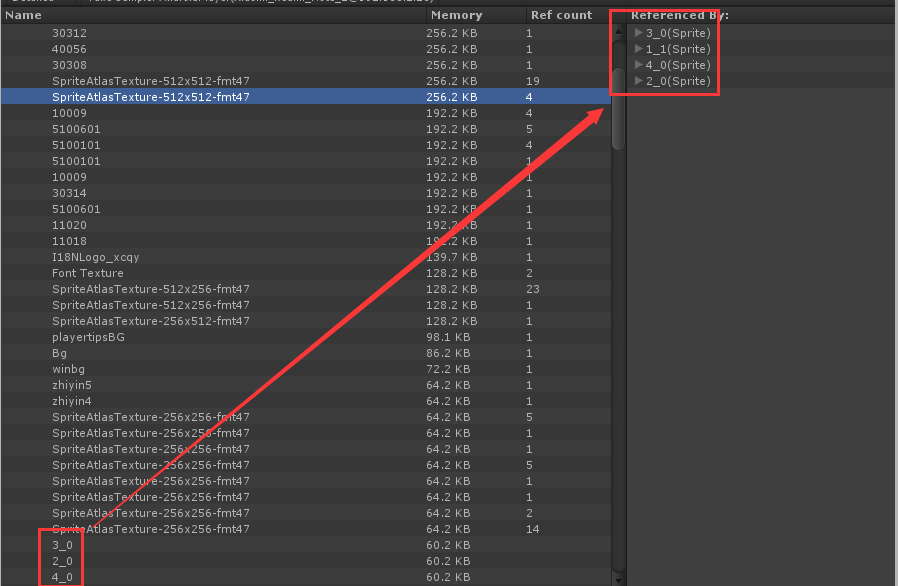
\includegraphics[width=.9\linewidth]{./pic/ugui4.png}
\end{center}
\begin{itemize}
\item 经过测试,这确实是 Unity 在 4.x 版本中的一个缺陷,理论上这张“新贴图(图集中的子图)”是不需要的,并不应该加载。 因此,我们建议通过以下方法来绕过该问题:
\item 在 assetBundle.Load (subFile, typeof (Sprite)) as Sprite; 之后,调用
\item Texture2D t = assetBundle.Load (subFile, typeof (Texture2D)) as Texture2D;
\item Resources.UnloadAsset(t);
\item 从而卸载这部分多余的内存。
\end{itemize}
\item 加载UI预制的时候,如果把特效放到预制里,会导致加载非常耗时。怎么优化这个加载时间呢?
\label{sec:org478c293}
\begin{itemize}
\item UI和特效(粒子系统)的加载开销在多数项目中都占据较高的CPU耗时。UI界面的实例化和加载耗时主要由以下几个方面构成:
\item 纹理资源加载耗时
\begin{itemize}
\item UI界面加载的主要耗时开销,因为在其资源加载过程中,时常伴有大量较大分辨率的Atlas纹理加载,我们在之前的Unity加载模块深度分析之纹理篇有详细讲解。对此,我们建议研发团队在美术质量允许的情况下,尽可能对UI纹理进行简化,从而加快UI界面的加载效率。
\end{itemize}

\begin{center}
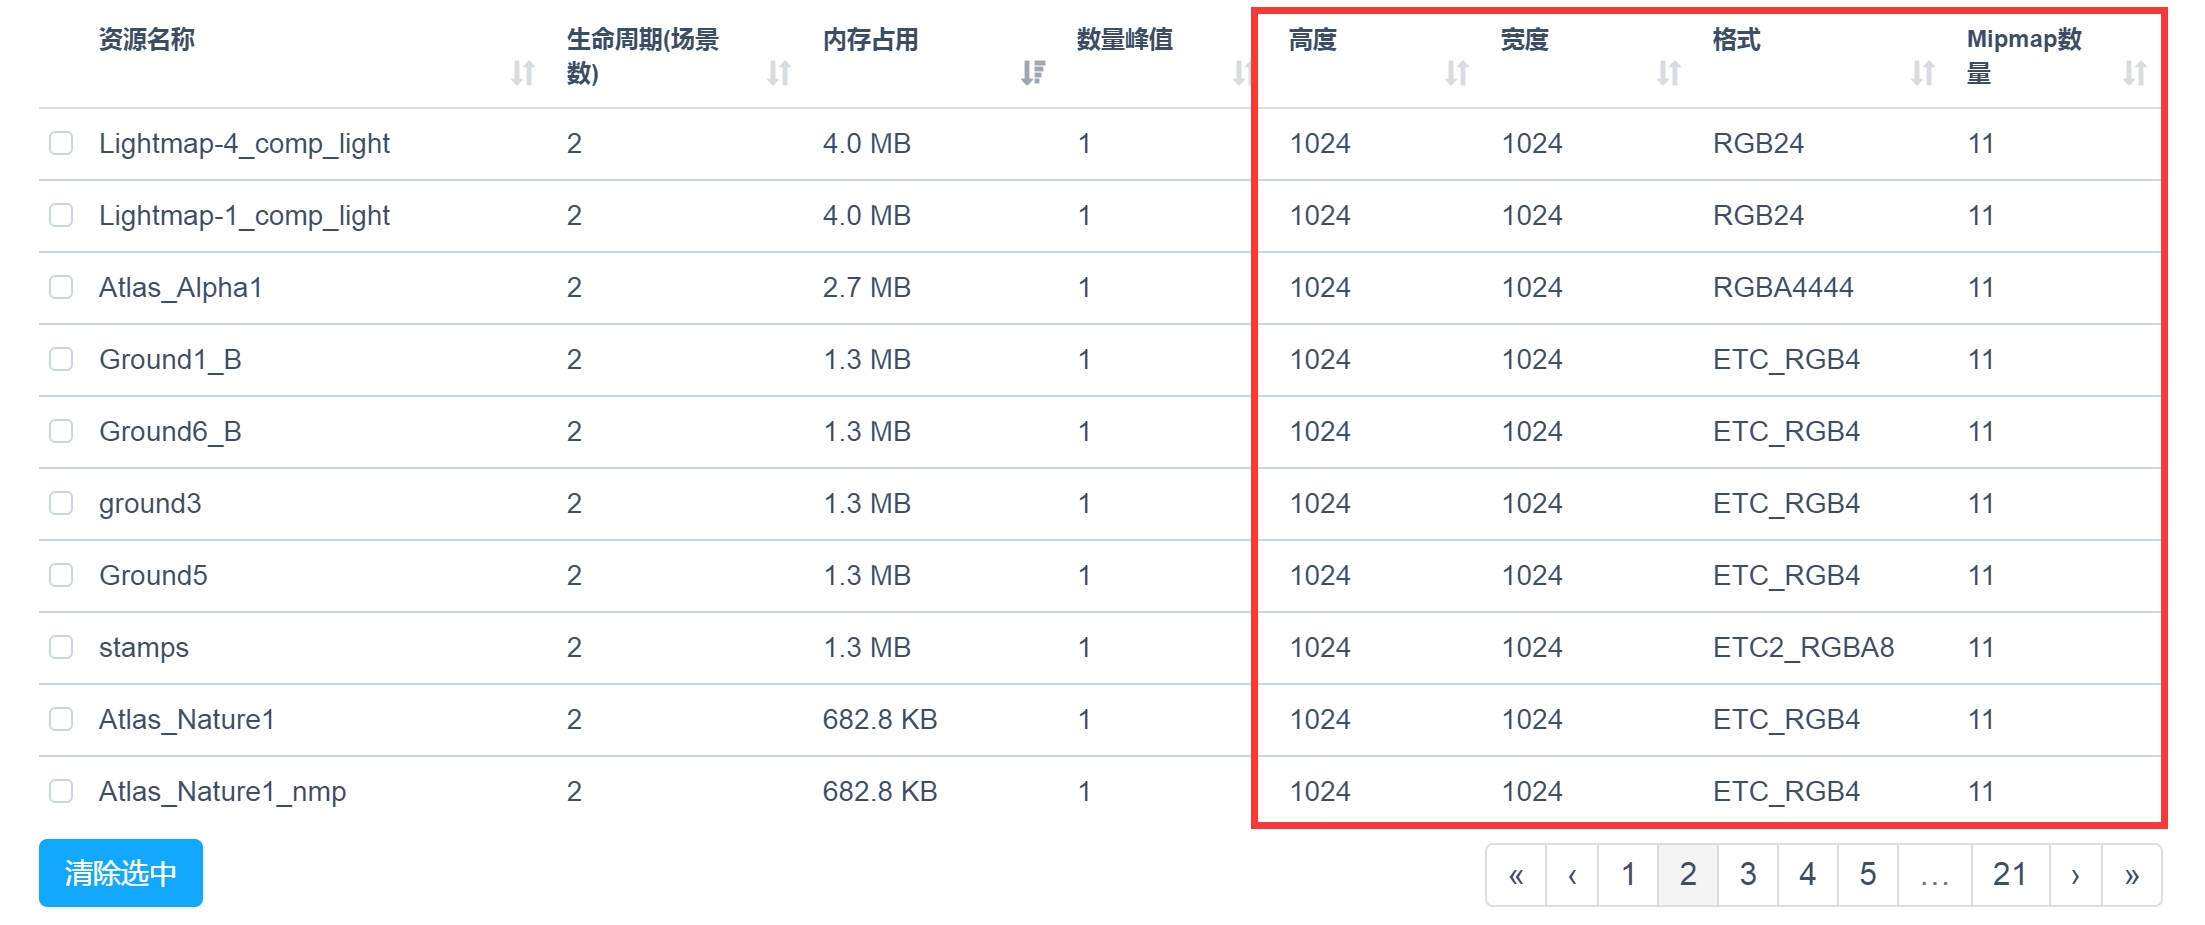
\includegraphics[width=.9\linewidth]{./pic/ugui5.jpg}
\end{center}
\item UI网格重建耗时
\begin{itemize}
\item UI界面在实例化或Active时,往往会造成Canvas(UGUI)或Panel(NGUI)中UIDrawCall的变化,进而触发网格重建操作。当Canvas或Panel中网格量较大时,其重建开销也会随之较大。
\end{itemize}
\item UI相关构造函数和初始化操作开销
\begin{itemize}
\item 这部分是指UI底层类在实例化时的ctor开销,以及OnEnable和OnDisable的自身开销。
\end{itemize}
\item 上述2和3主要为引擎或插件的自身逻辑开销,因此,我们应该尽可能避免或降低这两个操作的发生频率。我们的建议如下:
\begin{itemize}
\item 在内存允许的情况下,对于UI界面进行缓存。尽可能减少UI界面相关资源的重复加载以及相关类的重复初始化;
\item 根据UI界面的使用频率,使用更为合适的切换方式。比如移进移出或使用Culling Layer来实现UI界面的切换效果等,从而降低UI界面的加载耗时,提升切换的流畅度。
\item 对于特效(特别是粒子特效)来说,我们暂时并没有发现将UI界面和特效耦合在一起,其加载耗时会大于二者分别加载的耗时总和。因此,我们仅从优化粒子系统加载效率的角度来回答这个问题。粒子系统的加载开销,就目前来看,主要和其本身组件的反序列化耗时和加载数量相关。对于反序列化耗时而言,这是Unity引擎负责粒子系统的自身加载开销,开发者可以控制的空间并不大。对于加载数量,则是开发者需要密切关注的,因为在我们目前看到的项目中,不少都存在大量的粒子系统加载,有些项目的数量甚至超过1000个,如下图所示。因此,建议研发团队密切关注自身项目中粒子系统的数量使用情况。一般来说,建议我们建议粒子系统使用数量的峰值控制在400以下。
\end{itemize}

\begin{center}
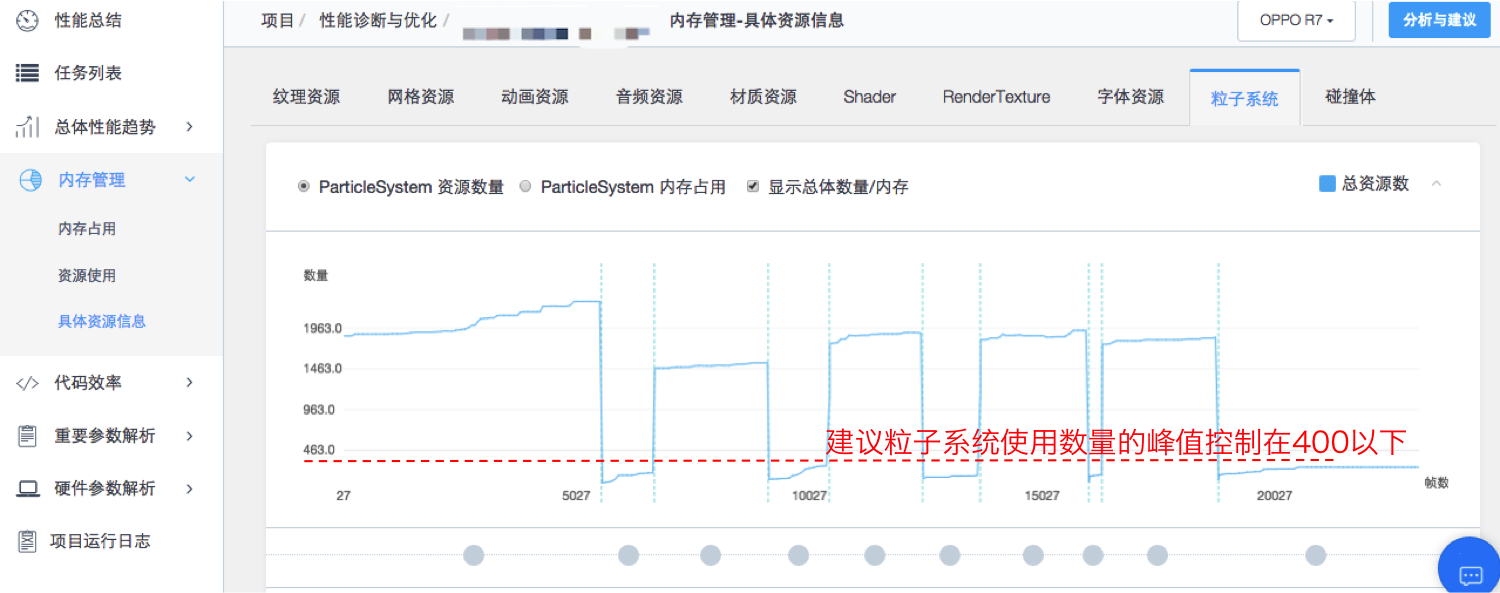
\includegraphics[width=.9\linewidth]{./pic/ugui6.png}
\end{center}
\end{itemize}
\item 我有一个UI预设,它使用了一个图集, 我在打包的时候把图集和UI一起打成了AssetBundle。我在加载生成了GameObject后立刻卸载了AssetBundle对象, 但是当我后面再销毁GameObject的时候发现图集依然存在,这是什么情况呢?
\label{sec:org94814b3}
\begin{itemize}
\item 这是很可能出现的。unload(false)卸载AssetBundle并不会销毁其加载的资源 ,是必须对其调用Resources.UnloadAsset,或者调用Resources.UnloadUnusedAssets才行。关于AssetBundle加载的详细解释可以参考我们之前的文章:你应该知道的AssetBundle管理机制。
\end{itemize}
\end{enumerate}
\subsubsection{字体相关}
\label{sec:org7521dc5}
\begin{enumerate}
\item 我在用Profiler真机查看iPhone App时,发现第一次打开某些UI时,Font.CacheFontForText占用时间超过2s,这块主要是由什么影响的?若iPhone5在这个接口消耗2s多,是不是问题很大?这个消耗和已经生成的RenderTexture的大小有关吗?
\label{sec:org87672e1}
\begin{itemize}
\item Font.CacheFontForText主要是指生成动态字体Font Texture的开销, 一次性打开UI界面中的文字越多,其开销越大。如果该项占用时间超过2s,那么确实是挺大的,这个消耗也与已经生成的Font Texture有关系。简单来说,它主要是看目前Font Texture中是否有地方可以容下接下来的文字,如果容不下才会进行一步扩大Font Texture,从而造成了性能开销。
\end{itemize}
\end{enumerate}

\section{Object Oriented Design/Programming and Design Patterns}
\label{sec:org42c3d85}
\subsection{设计模式的几个原则}
\label{sec:org6ff7c2a}
\begin{itemize}
\item \url{http://www.cnblogs.com/zhaoqingqing/p/4288454.html}
\item 原则1:单一职责
\item 原则2:里氏替换原则(子类扩展但不改变父类功能)
\item 原则3:依赖倒置原则
\item 原则4:接口隔离原则
\item 原则5:迪米特法则(最少知道原则)
\item 原则6:开闭原则
\end{itemize}
\subsubsection{原则1:单一职责原则}
\label{sec:org020d9a4}
\begin{itemize}
\item 说到单一职责原则,很多人都会不屑一顾。
\item 因为它太简单了,稍有经验的程序员即使从来没有读过设计模式、从来没有听说过单一职责原则,在设计软件时也会自觉的遵守这一重要原则,因为这是常识。
\item 在软件编程中,谁也不希望因为修改了一个功能导致其他的功能发生故障。
\item 而避免出现这一问题的方法便是遵循单一职责原则。
\item 虽然单一职责原则如此简单,并且被认为是常识,但是即便是经验丰富的程序员写出的程序,也会有违背这一原则的代码存在。
\item 为什么会出现这种现象呢?因为有职责扩散。所谓职责扩散,就是因为某种原因,职责被分化成了更细的职责。
\end{itemize}
\begin{enumerate}
\item 用一个类描述动物呼吸这个场景
\label{sec:org813e3f3}
\begin{minted}[linenos=true]{csharp}
class Animal {
    public void breathe(string animal) {
        Debug.Log(animal + "呼吸空气");
    }
}
public class Client {
    Animal animal = new Animal();
    void Start() {
        animal.breathe("牛");
        animal.breathe("羊");
        animal.breathe("猪");
    }
}
//运行结果:
//牛呼吸空气
//羊呼吸空气
//猪呼吸空气
\end{minted}

\item 当需求变动
\label{sec:orge6ba1cb}
\begin{itemize}
\item 程序上线后,发现问题了,并不是所有的动物都呼吸空气的,比如鱼就是呼吸水的。
\item 修改时如果遵循单一职责原则,需要将Animal类细分为陆生动物类Terrestrial,水生动物Aquatic,代码如下:
\end{itemize}
\begin{minted}[linenos=true]{csharp}
class Terrestrial {
    public void breathe(String animal) {
        Debug.Log(animal + "呼吸空气");
    }
}
class Aquatic {
    public void breathe(String animal) {
        Debug.Log(animal + "呼吸水");
    }
}
public class Client {
    public static void main(String[] args) {
        Terrestrial terrestrial = new Terrestrial();
        terrestrial.breathe("牛");
        terrestrial.breathe("羊");
        terrestrial.breathe("猪");
        Aquatic aquatic = new Aquatic();
        aquatic.breathe("鱼");
    }
}
//运行结果:
//牛呼吸空气
//羊呼吸空气
//猪呼吸空气
//鱼呼吸水
\end{minted}

\item 改动量小的方法
\label{sec:org4874138}
\begin{itemize}
\item 我们会发现如果这样修改花销是很大的,除了将原来的类分解之外,还需要修改客户端。
\item 而直接修改类Animal来达成目的虽然违背了单一职责原则,但花销却小的多,代码如下:
\begin{minted}[linenos=true]{csharp}
class Animal {
    public void breathe(String animal) {
        if ("鱼" == animal) {
            Debug.Log((animal + "呼吸水"));
        }
        else {
            Debug.Log((animal + "呼吸空气"));
        }
    }
}
public class Client {
    public static void main(String[] args) {
        Animal animal = new Animal();
        animal.breathe("牛");
        animal.breathe("羊");
        animal.breathe("猪");
        animal.breathe("鱼");
    }
}
\end{minted}
\end{itemize}
\item 隐患
\label{sec:org253a2a6}
\begin{itemize}
\item 可以看到,这种修改方式要简单的多。
\item 但是却存在着隐患:有一天需要将鱼分为呼吸淡水的鱼和呼吸海水的鱼,
\item 则又需要修改Animal类的breathe方法,而对原有代码的修改会对调用“猪”“牛”“羊”等相关功能带来风险,
\item 也许某一天你会发现程序运行的结果变为“牛呼吸水”了。
\item 这种修改方式直接在代码级别上违背了单一职责原则,虽然修改起来最简单,但隐患却是最大的。
\end{itemize}
\item 另一种修改方式
\label{sec:org18f4646}
\begin{minted}[linenos=true]{csharp}
class Animal {
    public void breathe(String animal) {
        Debug.Log(animal + "呼吸空气");
    }
    public void breathe2(String animal) {
        Debug.Log(animal + "呼吸水");
    }
}
public class Client {
    public static void main(String[] args) {
        Animal animal = new Animal();
        animal.breathe("牛");
        animal.breathe("羊");
        animal.breathe("猪");
        animal.breathe2("鱼");
    }
}
\end{minted}
\begin{itemize}
\item 可以看到,这种修改方式没有改动原来的方法,而是在类中新加了一个方法,这样虽然也违背了单一职责原则,
\item 但在方法级别上却是符合单一职责原则的,因为它并没有动原来方法的代码。这三种方式各有优缺点,
\item 那么在实际编程中,采用哪一中呢?
\item 其实这真的比较难说,需要根据实际情况来确定。
\item 我的原则是:只有逻辑足够简单,才可以在代码级别上违反单一职责原则;只有类中方法数量足够少,才可以在方法级别上违反单一职责原则。
\end{itemize}
\item 遵循单一职责原的优点有
\label{sec:org189e442}
\begin{itemize}
\item 可以降低类的复杂度,一个类只负责一项职责,其逻辑肯定要比负责多项职责简单的多;
\item 提高类的可读性,提高系统的可维护性;
\item 变更引起的风险降低,变更是必然的,如果单一职责原则遵守的好,当修改一个功能时,可以显著降低对其他功能的影响。
\item 需要说明的一点是单一职责原则不只是面向对象编程思想所特有的,只要是模块化的程序设计,都适用单一职责原则。
\end{itemize}
\end{enumerate}
\subsubsection{原则2:里氏替换原则}
\label{sec:orgd02ade0}
\begin{enumerate}
\item 名字的由来
\label{sec:org0d2d2d6}
\begin{itemize}
\item 肯定有不少人跟我刚看到这项原则的时候一样,对这个原则的名字充满疑惑。
\item 其实原因就是这项原则最早是在1988年,由麻省理工学院的一位姓里的女士(Barbara Liskov)提出来的。
\item 简单来说的话,就是当我们使用继承时,遵循里氏替换原则。
\end{itemize}
\item 定义
\label{sec:orgce139c8}
\begin{itemize}
\item 注:类B继承类A时,除添加新的方法完成新增功外,尽量不要重写父类A的方法,也尽量不要重载父类A的方法。
\item 继承包含这样一层含义:父类中凡是已经实现好的方法(相对于抽象方法而言),实际上是在设定一系列的规范和契约,
\item 虽然它不强制要求所有的子类必须遵从这些契约,但是如果子类对这些非抽象方法任意修改,
\item 就会对整个继承体系造成破坏。而里氏替换原则就是表达了这一层含义。
\item 继承作为面向对象三大特性之一,在给程序设计带来巨大便利的同时,也带来了弊端。
\item 比如使用继承会给程序带来侵入性,程序的可移植性降低,增加了对象间的耦合性,如果一个类被其他的类所继承,
\item 则当这个类需要修改时,必须考虑到所有的子类,并且父类修改后,
\item 所有涉及到子类的功能都有可能会产生故障。
\end{itemize}
\item 继承的风险
\label{sec:orgc6193ee}
\begin{itemize}
\item 那就让我们一起看看继承的风险,如下:
\begin{minted}[linenos=true]{csharp}
class A {
    public int func1(int a, int b) {
        return a - b;
    }
}
public class Client {
    void Start() {
        A a = new A();
        Debug.Log("100-50=" + a.func1(100, 50));
        Debug.Log("100-80=" + a.func1(100, 80));
    }
}
// 运行结果
// 100-50=50 
// 100-80=20
\end{minted}
\end{itemize}
\item 需求变动
\label{sec:orga4402eb}
\begin{itemize}
\item 后来,我们需要增加一个新的功能:完成两数相加,然后再与100求和,由类B来负责。
\item 即类B需要完成两个功能:
\item 两数相减。
\item 两数相加,然后再加100。
\item 由于类A已经实现了第一个功能,所以类B继承类A后,只需要再完成第二个功能就可以了,代码如下 
\begin{minted}[linenos=true]{csharp}
class B:A {
    public int func1(int a, int b) {
        return a + b;
    }
    public int func2(int a, int b) {
        return func1(a, b) + 100;
    }
}
public class Client {
    private void Start() {
        B b = new B();
        Debug.Log("100-50=" + b.func1(100, 50));
        Debug.Log("100-80=" + b.func1(100, 80));
        Debug.Log("100+20+100=" + b.func2(100, 20));
    }
}
// 类B运行结果
// 100-50=150 
// 100-80=180 
// 100+20+100=220
\end{minted}
\end{itemize}
\item 影响了正常的功能
\label{sec:orgac29381}
\begin{itemize}
\item 我们发现原本运行正常的相减功能发生了错误。
\item 原因就是类B在给方法起名时无意中重写了父类的方法,造成所有运行相减功能的代码全部调用了类B重写后的方法,造成原本运行正常的功能出现了错误。
\item 在本例中,引用基类A完成的功能,换成子类B之后,发生了异常。
\item 在实际编程中,我们常常会通过重写父类的方法来完成新的功能,这样写起来虽然简单,
\item 但是整个继承体系的可复用性会比较差,特别是运用多态比较频繁时,程序运行出错的几率非常大。
\item 如果非要重写父类的方法,比较通用的做法是:原来的父类和子类都继承一个更通俗的基类,原有的继承关系去掉,采用依赖、聚合,组合等关系代替。
\end{itemize}
\item 里氏替换原则通俗的来讲就是
\label{sec:org6784a67}
\begin{itemize}
\item 子类可以扩展父类的功能,但不能改变父类原有的功能。它包含以下4层含义:
\item 1.子类可以实现父类的抽象方法,但不能覆盖父类的非抽象方法。
\item 2.子类中可以增加自己特有的方法。
\item 3.当子类的方法重载父类的方法时,方法的前置条件(即方法的形参)要比父类方法的输入参数更宽松。
\item 4.当子类的方法实现父类的抽象方法时,方法的后置条件(即方法的返回值)要比父类更严格。
\item 看上去很不可思议,因为我们会发现在自己编程中常常会违反里氏替换原则,程序照样跑的好好的。
\item 所以大家都会产生这样的疑问,假如我非要不遵循里氏替换原则会有什么后果?
\item 后果就是:你写的代码出问题的几率将会大大增加。
\end{itemize}
\end{enumerate}
\subsubsection{原则3:依赖倒置原则}
\label{sec:org958bd2b}
\begin{enumerate}
\item 定义
\label{sec:orgb7f6275}
\begin{itemize}
\item 高层模块不应该依赖低层模块,二者都应该依赖其抽象;抽象不应该依赖细节;细节应该依赖抽象。
\item 以抽象为基础搭建起来的架构比以细节为基础搭建起来的架构要稳定的多。
\item 抽象指的是接口或者抽象类,细节就是具体的实现类,使用接口或者抽象类的目的是制定好规范和契约,而不去涉及任何具体的操作,把展现细节的任务交给他们的实现类去完成。
\end{itemize}
\item 依赖倒置原则核心思想
\label{sec:orgbdbbc52}
\begin{itemize}
\item 依赖倒置原则的核心思想是面向接口编程,我们依旧用一个例子来说明面向接口编程比相对于面向实现编程好在什么地方。
\end{itemize}
\item 情景举例
\label{sec:org84bb94a}
\begin{itemize}
\item 场景是这样的,母亲给孩子讲故事,只要给她一本书,她就可以照着书给孩子讲故事了。代码如下:
\begin{minted}[linenos=true]{csharp}
class Book {
    public String getContent() {
        return "很久很久以前有一个阿拉伯的故事……";
    }
}
class Mother {
    public void narrate(Book book) {
        Debug.Log("妈妈开始讲故事");
        Debug.Log(book.getContent());
    }
}
public class Client {
    void Start() {
        Mother mother = new Mother();
        mother.narrate(new Book());
    }
}
// 运行结果:
// 妈妈开始讲故事 
// 很久很久以前有一个阿拉伯的故事……
\end{minted}
\end{itemize}
\item 需求变动
\label{sec:org9e6be89}
\begin{itemize}
\item 运行良好,假如有一天,需求变成这样:不是给书而是给一份报纸,让这位母亲讲一下报纸上的故事,报纸的代码如下:
\begin{minted}[linenos=true]{csharp}
class Newspaper {
    public String getContent() {
        return "林书豪38+7领导尼克斯击败湖人……";
    }
}
\end{minted}
\item 这位母亲却办不到,因为她居然不会读报纸上的故事,这太荒唐了,只是将书换成报纸,居然必须要修改Mother才能读。
\item 假如以后需求换成杂志呢?换成网页呢?
\item 还要不断地修改Mother,这显然不是好的设计。
\item 原因就是Mother与Book之间的耦合性太高了,必须降低他们之间的耦合度才行。
\end{itemize}
\item 抽象的接口
\label{sec:orgbc2132e}
\begin{itemize}
\item 我们引入一个抽象的接口IReader。
\item 读物,只要是带字的都属于读物:
\begin{minted}[linenos=true]{csharp}
interface IReader {
    String getContent();
}
\end{minted}
\item Mother类与接口IReader发生依赖关系,而Book和Newspaper都属于读物的范畴,
\item 他们各自都去实现IReader接口,这样就符合依赖倒置原则了,代码修改为:
\begin{minted}[linenos=true]{csharp}
interface IReader {
    String getContent();
}
class Newspaper : IReader {
    public String getContent() {
        return "林书豪17+9助尼克斯击败老鹰……";
    }
}
class Book : IReader {
    public String getContent() {
        return "很久很久以前有一个阿拉伯的故事……";
    }
}
class Mother {
    public void narrate(IReader reader) {
        Debug.Log("妈妈开始讲故事");
        Debug.Log(reader.getContent());
    }
}
public class Client {
    public static void main(String[] args) {
        Mother mother = new Mother();
        mother.narrate(new Book());
        mother.narrate(new Newspaper());
    }
}
// 运行结果
// 妈妈开始讲故事 
// 很久很久以前有一个阿拉伯的故事…… 
// 妈妈开始讲故事 
// 林书豪17+9助尼克斯击败老鹰……
\end{minted}
\end{itemize}
这样修改后,无论以后怎样扩展Client类,都不需要再修改Mother类了。 
\begin{itemize}
\item 这只是一个简单的例子,实际情况中,代表高层模块的Mother类将负责完成主要的业务逻辑,一旦需要对它进行修改,引入错误的风险极大。
\item 所以遵循依赖倒置原则可以降低类之间的耦合性,提高系统的稳定性,降低修改程序造成的风险。
\item 采用依赖倒置原则给多人并行开发带来了极大的便利,
\item 比如上例中,原本Mother类与Book类直接耦合时,Mother类必须等Book类编码完成后才可以进行编码,因为Mother类依赖于Book类。
\item 修改后的程序则可以同时开工,互不影响,因为Mother与Book类一点关系也没有。
\item 参与协作开发的人越多、项目越庞大,采用依赖导致原则的意义就越重大。
\item 现在很流行的TDD开发模式就是依赖倒置原则最成功的应用。
\end{itemize}
\item 在实际编程中,我们一般需要做到如下3点
\label{sec:org5f83d26}
\begin{itemize}
\item 1.低层模块尽量都要有抽象类或接口,或者两者都有。
\item 2.变量的声明类型尽量是抽象类或接口。使用继承时遵循里氏替换原则。
\item 3.依赖倒置原则的核心就是要我们面向接口编程,理解了面向接口编程,也就理解了依赖倒置。
\end{itemize}
\end{enumerate}
\subsubsection{原则4:接口隔离原则}
\label{sec:orge9a1ee9}
\begin{enumerate}
\item 定义
\label{sec:org3787a71}
\begin{itemize}
\item 客户端不应该依赖它不需要的接口;一个类对另一个类的依赖应该建立在最小的接口上。
\item 将臃肿的接口I拆分为独立的几个接口,类A和类C分别与他们需要的接口建立依赖关系。也就是采用接口隔离原则。
\item 举例来说明接口隔离原则:
\end{itemize}
\item 未遵循接口隔离原则的设计
\label{sec:orgd12e5d5}
\begin{itemize}
\item 类图1
\item 这个图的意思是:类A依赖接口I中的方法1、方法2、方法3,类B是对类A依赖的实现。
\item 类C依赖接口I中的方法1、方法4、方法5,类D是对类C依赖的实现。
\item 对于类B和类D来说,虽然他们都存在着用不到的方法(也就是图中红色字体标记的方法),但由于实现了接口I,所以也必须要实现这些用不到的方法。
\end{itemize}
\item 示例代码
\label{sec:org35bfe3d}
\begin{itemize}
\item 对类图不熟悉的可以参照程序代码来理解,代码如下:
\begin{minted}[linenos=true]{csharp}
//接口
interface I {
    void method1();
    void method2();
    void method3();
    void method4();
    void method5();
}

class A {
    public void depend1(I i) {
        i.method1();
    }
    public void depend2(I i) {
        i.method2();
    }
    public void depend3(I i) {
        i.method3();
    }
}

class B : I {
    public void method1() {
        Debug.Log("类B实现接口I的方法1");
    }
    public void method2() {
        Debug.Log("类B实现接口I的方法2");
    }
    public void method3() {
        Debug.Log("类B实现接口I的方法3");
    }
    //对于类B来说,method4和method5不是必需的,但是由于接口A中有这两个方法,
    //所以在实现过程中即使这两个方法的方法体为空,也要将这两个没有作用的方法进行实现。
    public void method4() { }
    public void method5() { }
}

class C {
    public void depend1(I i) {
        i.method1();
    }
    public void depend2(I i) {
        i.method4();
    }
    public void depend3(I i) {
        i.method5();
    }
}

class D : I {
    public void method1() {
        Debug.Log("类D实现接口I的方法1");
    }
    //对于类D来说,method2和method3不是必需的,但是由于接口A中有这两个方法,
    //所以在实现过程中即使这两个方法的方法体为空,也要将这两个没有作用的方法进行实现。
    public void method2() { }
    public void method3() { }
    public void method4() {
        Debug.Log("类D实现接口I的方法4");
    }
    public void method5() {
        Debug.Log("类D实现接口I的方法5");
    }
}

public class Client {
    void Start() {
        A a = new A();
        a.depend1(new B());
        a.depend2(new B());
        a.depend3(new B());
        C c = new C();
        c.depend1(new D()));
        c.depend2(new D());
        c.depend3(new D());
    }
}
\end{minted}
\item 可以看到,如果接口过于臃肿,只要接口中出现的方法,不管对依赖于它的类有没有用处,实现类中都必须去实现这些方法,这显然不是好的设计。
\item 如果将这个设计修改为符合接口隔离原则,就必须对接口I进行拆分。
\end{itemize}
\item 遵循接口隔离原则的设计
\label{sec:org2a4585a}
\begin{itemize}
\item 在这里我们将原有的接口I拆分为三个接口,拆分后的设计如图2所示:
\item 类图2
\end{itemize}
\item 示例代码
\label{sec:orgdf4a9d3}
\begin{itemize}
\item 照例贴出程序的代码,供不熟悉类图的朋友参考:
\begin{minted}[linenos=true]{csharp}
interface I1 {
    void method1();
}

interface I2 {
    void method2();
    void method3();
}

interface I3 {
    void method4();
    void method5();
}

class A {
    public void depend1(I1 i) {
        i.method1();
    }
    public void depend2(I2 i) {
        i.method2();
    }
    public void depend3(I2 i) {
        i.method3();
    }
}

class B : I1, I2 {
    public void method1() {
        Debug.Log("类B实现接口I1的方法1");
    }
    public void method2() {
        Debug.Log("类B实现接口I2的方法2");
    }
    public void method3() {
        Debug.Log("类B实现接口I2的方法3");
    }
}

class C {
    public void depend1(I1 i) {
        i.method1();
    }
    public void depend2(I3 i) {
        i.method4();
    }
    public void depend3(I3 i) {
        i.method5();
    }
}

class D : I1, I3 {
    public void method1() {
        Debug.Log("类D实现接口I1的方法1");
    }
    public void method4() {
        Debug.Log("类D实现接口I3的方法4");
    }
    public void method5() {
        Debug.Log("类D实现接口I3的方法5");
    }
}
\end{minted}
\item 接口隔离原则的含义是:建立单一接口,不要建立庞大臃肿的接口,尽量细化接口,接口中的方法尽量少。
\item 也就是说,我们要为各个类建立专用的接口,而不要试图去建立一个很庞大的接口供所有依赖它的类去调用。
\item 本文例子中,将一个庞大的接口变更为3个专用的接口所采用的就是接口隔离原则。
\item 在程序设计中,依赖几个专用的接口要比依赖一个综合的接口更灵活。
\item 接口是设计时对外部设定的“契约”,通过分散定义多个接口,可以预防外来变更的扩散,提高系统的灵活性和可维护性。
\item 说到这里,很多人会觉的接口隔离原则跟之前的单一职责原则很相似,其实不然。
\item 其一,单一职责原则原注重的是职责;而接口隔离原则注重对接口依赖的隔离。
\item 其二,单一职责原则主要是约束类,其次才是接口和方法,它针对的是程序中的实现和细节;
\item 而接口隔离原则主要约束接口,主要针对抽象,针对程序整体框架的构建。
\end{itemize}
\item 注意几点
\label{sec:org62a1339}
\begin{itemize}
\item 采用接口隔离原则对接口进行约束时,要注意以下几点:
\item 1.接口尽量小,但是要有限度。对接口进行细化可以提高程序设计灵活性是不挣的事实,但是如果过小,则会造成接口数量过多,使设计复杂化。所以一定要适度。
\item 2.为依赖接口的类定制服务,只暴露给调用的类它需要的方法,它不需要的方法则隐藏起来。只有专注地为一个模块提供定制服务,才能建立最小的依赖关系。
\item 3.提高内聚,减少对外交互。使接口用最少的方法去完成最多的事情。
\item 运用接口隔离原则,一定要适度,接口设计的过大或过小都不好。设计接口的时候,只有多花些时间去思考和筹划,才能准确地实践这一原则。
\item 
\end{itemize}
\end{enumerate}
\subsubsection{原则5:迪米特法则}
\label{sec:orgd5ab4d0}
\begin{enumerate}
\item 定义
\label{sec:orga2f5b92}
\begin{itemize}
\item 一个对象应该对其他对象保持最少的了解
\item 类与类之间的关系越密切,耦合度越大,当一个类发生改变时,对另一个类的影响也越大。
\item 因此,尽量降低类与类之间的耦合。
\item 自从我们接触编程开始,就知道了软件编程的总的原则:低耦合,高内聚。
\item 无论是面向过程编程还是面向对象编程,只有使各个模块之间的耦合尽量的低,才能提高代码的复用率。
\item 低耦合的优点不言而喻,但是怎么样编程才能做到低耦合呢?那正是迪米特法则要去完成的。
\end{itemize}
\item 最少知道原则
\label{sec:org2ca0fdc}
\begin{itemize}
\item 迪米特法则又叫最少知道原则,最早是在1987年由美国Northeastern University的Ian Holland提出。
\item 通俗的来讲,就是一个类对自己依赖的类知道的越少越好。也就是说,对于被依赖的类来说,无论逻辑多么复杂,都尽量地的将逻辑封装在类的内部,对外除了提供的public方法,不对外泄漏任何信息。
\item 迪米特法则还有一个更简单的定义:只与直接的朋友通信。首先来解释一下什么是直接的朋友:
\item 每个对象都会与其他对象有耦合关系,只要两个对象之间有耦合关系,我们就说这两个对象之间是朋友关系。
\item 耦合的方式很多,依赖、关联、组合、聚合等。其中,我们称出现成员变量、方法参数、方法返回值中的类为直接的朋友,
\item 而出现在局部变量中的类则不是直接的朋友。也就是说,陌生的类最好不要作为局部变量的形式出现在类的内部。
\end{itemize}
\item 违反迪米特法则的设计
\label{sec:org354aa02}
\begin{itemize}
\item 举一个例子:有一个集团公司,下属单位有分公司和直属部门,现在要求打印出所有下属单位的员工ID。
\item 先来看一下违反迪米特法则的设计。
\begin{minted}[linenos=true]{csharp}
//总公司员工
class Employee {
    private String id;
    public void setId(String id) {
        this.id = id;
    }
    public String getId() {
        return id;
    }
}

//分公司员工
class SubEmployee {
    private String id;
    public void setId(String id) {
        this.id = id;
    }
    public String getId() {
        return id;
    }
}

class SubCompanyManager {
    public List<SubEmployee> getAllEmployee() {
        List<SubEmployee> list = new List<SubEmployee>();
        for (int i = 0; i < 100; i++) {
            SubEmployee emp = new SubEmployee();
            //为分公司人员按顺序分配一个ID
            emp.setId("分公司" + i);
            list.Add(emp);
        }
        return list;
    }
}

class CompanyManager {
    public List<Employee> getAllEmployee() {
        List<Employee> list = new List<Employee>();
        for (int i = 0; i < 30; i++) {
            Employee emp = new Employee();
            //为总公司人员按顺序分配一个ID
            emp.setId("总公司" + i);
            list.Add(emp);
        }
        return list;
    }
    public void printAllEmployee(SubCompanyManager sub) {
        List<SubEmployee> list1 = sub.getAllEmployee();
        foreach (SubEmployee e in list1) {
            Debug.Log(e.getId());
        }
        List<Employee> list2 = this.getAllEmployee();
        foreach (Employee e in list2) {
            Debug.Log(e.getId());
        }
    }
}

public class Client {
    void Start() {
        CompanyManager e = new CompanyManager();
        e.printAllEmployee(new SubCompanyManager());
    }
}
\end{minted}
\item 现在这个设计的主要问题出在CompanyManager中,根据迪米特法则,只与直接的朋友发生通信,
\item 而SubEmployee类并不是CompanyManager类的直接朋友(以局部变量出现的耦合不属于直接朋友),从逻辑上讲总公司只与他的分公司耦合就行了,
\item 与分公司的员工并没有任何联系,这样设计显然是增加了不必要的耦合。
\end{itemize}
\item 修改后的代码
\label{sec:org5ac68bc}
\begin{itemize}
\item 按照迪米特法则,应该避免类中出现这样非直接朋友关系的耦合。修改后的代码如下:
\begin{minted}[linenos=true]{csharp}
class SubCompanyManager {
    public List<SubEmployee> getAllEmployee() {
        List<SubEmployee> list = new List<SubEmployee>();
        for (int i = 0; i < 100; i++) {
            SubEmployee emp = new SubEmployee();
            //为分公司人员按顺序分配一个ID
            emp.setId("分公司" + i);
            list.Add(emp);
        }
        return list;
    }
    public void printEmployee() {
        List<SubEmployee> list = this.getAllEmployee();
        foreach (SubEmployee e in list) {
            Debug.Log(e.getId());
        }
    }
}

class CompanyManager {
    public List<Employee> getAllEmployee() {
        List<Employee> list = new List<Employee>();
        for (int i = 0; i < 30; i++) {
            Employee emp = new Employee();
            //为总公司人员按顺序分配一个ID
            emp.setId("总公司" + i);
            list.Add(emp);
        }
        return list;
    }
    public void printAllEmployee(SubCompanyManager sub) {
        sub.printEmployee();
        List<Employee> list2 = this.getAllEmployee();
        foreach (Employee e in list2) {
            Debug.Log(e.getId());
        }
    }
}
\end{minted}
\end{itemize}
\item 主要的变化
\label{sec:org314429a}
\begin{itemize}
\item 修改后,为分公司增加了打印人员ID的方法,总公司直接调用来打印,从而避免了与分公司的员工发生耦合。
\end{itemize}
\item 总结
\label{sec:orgac9da99}
\begin{itemize}
\item 迪米特法则的初衷是降低类之间的耦合,由于每个类都减少了不必要的依赖,因此的确可以降低耦合关系。
\item 但是凡事都有度,虽然可以避免与非直接的类通信,但是要通信,必然会通过一个“中介”来发生联系,例如本例中,
\item 总公司就是通过分公司这个“中介”来与分公司的员工发生联系的。
\item 过分的使用迪米特原则,会产生大量这样的中介和传递类,导致系统复杂度变大。
\item 所以在采用迪米特法则时要反复权衡,既做到结构清晰,又要高内聚低耦合。
\end{itemize}
\end{enumerate}

\subsubsection{原则6:开闭原则}
\label{sec:org98aa141}
\begin{enumerate}
\item 定义
\label{sec:orga1f22a8}
\begin{itemize}
\item 一个软件实体如类、模块和函数应该对扩展开放,对修改关闭
\item 在软件的生命周期内,因为变化、升级和维护等原因需要对软件原有代码进行修改时,
\item 可能会给旧代码中引入错误,也可能会使我们不得不对整个功能进行重构,并且需要原有代码经过重新测试。
\item 因此,当软件需要变化时,尽量通过扩展软件实体的行为来实现变化,而不是通过修改已有的代码来实现变化。
\item 闭原则是面向对象设计中最基础的设计原则,它指导我们如何建立稳定灵活的系统。开闭原则可能是设计模式六项原则中定义最模糊的一个了,
\item 它只告诉我们对扩展开放,对修改关闭,可是到底如何才能做到对扩展开放,对修改关闭,并没有明确的告诉我们。
\item 以前,如果有人告诉我“你进行设计的时候一定要遵守开闭原则”,我会觉的他什么都没说,但貌似又什么都说了。因为开闭原则真的太虚了。
\item 在仔细思考以及仔细阅读很多设计模式的文章后,终于对开闭原则有了一点认识。
\item 其实,我们遵循设计模式前面5大原则,以及使用23种设计模式的目的就是遵循开闭原则。
\end{itemize}
\item 如何遵守
\label{sec:org0e26f0d}
\begin{itemize}
\item 也就是说,只要我们对前面5项原则遵守的好了,设计出的软件自然是符合开闭原则的,这个开闭原则更像是前面五项原则遵守程度的“平均得分”,
\item 前面5项原则遵守的好,平均分自然就高,说明软件设计开闭原则遵守的好;
\item 如果前面5项原则遵守的不好,则说明开闭原则遵守的不好。
\item 其实,开闭原则无非就是想表达这样一层意思:用抽象构建框架,用实现扩展细节。
\item 因为抽象灵活性好,适应性广,只要抽象的合理,可以基本保持软件架构的稳定。
\item 而软件中易变的细节,我们用从抽象派生的实现类来进行扩展,当软件需要发生变化时,我们只需要根据需求重新派生一个实现类来扩展就可以了。
\item 当然前提是我们的抽象要合理,要对需求的变更有前瞻性和预见性才行。
\end{itemize}
\end{enumerate}
\subsubsection{如何去遵守这六个原则}
\label{sec:org33e015d}
\begin{itemize}
\item 对这六个原则的遵守并不是 是和否的问题,而是多和少的问题,也就是说,我们一般不会说有没有遵守,而是说遵守程度的多少。
\item 任何事都是过犹不及,设计模式的六个设计原则也是一样,制定这六个原则的目的并不是要我们刻板的遵守他们,而需要根据实际情况灵活运用。
\item 对他们的遵守程度只要在一个合理的范围内,就算是良好的设计。
\item 如果大家对这六项原则的理解跟我有所不同,欢迎指正
\end{itemize}


\subsection{Unity中各种设计模式的实践与运用}
\label{sec:org7a5649a}
\begin{itemize}
\item \url{https://blog.csdn.net/u010019717/article/details/41172783}
\item \url{https://www.ctolib.com/Unity-Design-Pattern.html}
\item 23 design patterns.
\end{itemize}
\begin{center}
\begin{tabular}{lll}
\hline
 & 1. Abstract Factory 抽象工厂 & 创建几个相似的类的一个实例\\
 & 2. Builder 生成器 & 分离对象构造与它的表示\\
Creational Patterns & 3. Factory Method 工厂方法 & 创建几个派生类的一个实例\\
 & 4. Prototype 原型 & 要复制或克隆一个完全初始化的实例\\
 & 5. Singleton 单件 & 一个类只能运行一个实例可以存在\\
\hline
 & 6. Adapter 适配器 & 不同的类的接口相匹配\\
 & 7. Bridge 桥接 & 从其实现分离对象接口\\
 & 8. Composite 复合 & 简单和复合对象的树形结构\\
Structural Patterns & 9 .Decorator 装饰者 & 动态添加到对象的责任\\
 & 10. Facade 外观 & 一个表示整个子系统的单个类\\
 & 11. Flyweight 享元 & 细粒度的实例用于高效共享\\
 & 12. Proxy 代理服务器 & 一个表示另一个对象的对象\\
\hline
 & 13. Chain of Resp. 职责链模式 & 一连串的对象之间传递请求的一种方式\\
 & 14. Command 命令 & 将命令请求封装为一个对象\\
 & 15. Interpreter 解释器 & 方法包含程序中的语言元素\\
 & 16. Iterator 迭代器 & 按顺序访问集合中的元素\\
 & 17. Mediator 中介者 & 定义简化的类之间的通信\\
Behavioral Patterns & 18. Memento 备忘录 & 捕获和还原对象的内部状态\\
 & 19. Observer 观察者 & 一种方式通知到类数目的变化\\
 & 20. State 状态 & 在其状态改变时,改变一个对象的行为\\
 & 21. Strategy 策略 & 封装在类的内部算法\\
 & 22. Template Method 模板方法 & 推迟算法到子类的确切步骤\\
 & 23. Visitor 访问者 & 对一类没有改变定义新的操作\\
\hline
\end{tabular}
\end{center}

\subsubsection{Gang of Four Patterns in Unity (23种GOF设计模式的Unity实现)}
\label{sec:orgda8c6b0}
\begin{enumerate}
\item Behavioral Patterns 行为型模式
\label{sec:org6dfb622}
Command Pattern 命令模式
\begin{itemize}
\item State Pattern 状态模式
\item Observer Pattern 观察者模式
\item Chain of Responsibility Pattern 责任链模式
\item Mediator Pattern 中介者模式
\item Interpreter Pattern 解释器模式
\item Iterator Pattern 迭代器模式
\item Memento Pattern 备忘录模式
\item Strategy Pattern 策略模式
\item Template Method Pattern 模板方法模式
\item Visitor Pattern 访问者模式
\end{itemize}
\item Structural Patterns 结构型模式
\label{sec:org272d0fa}
\begin{itemize}
\item Adapter Pattern 适配器模式
\item Bridge Pattern 桥接模式
\item Composite Pattern 组合模式
\item Decorator Pattern 装饰模式
\item Facade Pattern 外观模式
\item Flyweight Pattern 享元模式
\item Proxy Pattern 代理模式
\end{itemize}
\item Creational Patterns 创建型模式
\label{sec:orgd84bc07}
\begin{itemize}
\item Prototype Pattern 原型模式
\item Singleton Pattern 单例模式
\item Abstract Factory Pattern 抽象工厂模式
\item Builder Pattern 建造者模式
\item Factory Method Pattern 工厂方法模式
\end{itemize}
\end{enumerate}
\subsubsection{Game Programming Patterns in Unity (《游戏编程模式》的Unity实现)}
\label{sec:org26c3ae8}
\begin{itemize}
\item Subclass Sandbox Pattern 子类沙盒模式
\item Type Object Pattern 类型对象模式
\item Component Pattern 组件模式
\item Event Queue Pattern 事件队列模式
\item Game Loop Pattern 游戏循环模式
\item Service Locator Pattern 服务定位器模式
\item Data Locality Pattern 数据局部性模式
\item Dirty Flag Pattern 脏标记模式
\item Object Pool Pattern 对象池模式
\end{itemize}


\subsection{单例模式(Unity3D/C\#)}
\label{sec:orga6b8534}
\subsubsection{【单例概述】}
\label{sec:org4a2a56a}
\begin{itemize}
\item 定义:单例,顾名思义,单个实例,即应用单例模式的类有且只有一个实例对象,并提供一个全局访问点来共其他类与对象访问。
\item (1)有且只有一个实例对象。
\item 有实例对象说明该类不是抽象类;只有一个实例对象表示不能随时随地的new一个该类的对象出来(这不是对开发者的约定,而是代码层面上的约定,即如果你这样做了,编辑器会提示你错误),即该类的构造函数是private级别,只能在类的内部构建实例对象;
\item (2)提供全局访问点使其他类与对象访问。
\item 这说明应用单例模式的类在提供实例访问方法时,该方法应该是静态的。
\item 有了如上的分析,就可以很轻松的创建单例类了,代码并不是很复杂。为什么要分成“C\#中的单例模式”和“Unity中的伪单例模式”,前者指C\#语言本身,后者指在Unity的Mono框架下。还有一点要说的,下面所有所有的例子都只是说明单例如何创建,不是说类中就这么点东西。。。- -
\end{itemize}
\subsubsection{【C\#中的单例模式】}
\label{sec:org6edd41f}
\begin{itemize}
\item 在单例模式中,根据应用情况的不同,也有着不同的实现方式。先把统一的访问方式写出来,这种访问方式应用于该命题下述的所有模式。
\begin{minted}[linenos=true]{csharp}
namespace CSharpTest {
    class Program {
        static void Main(string[] args) {
            Singleton s = Singleton.GetInstance();
        }
    }
}
\end{minted}
\end{itemize}
\begin{enumerate}
\item 饿汉模式
\label{sec:org553a765}
\begin{itemize}
\item 意思是,在该类装载时构建类的单例。(类的装载可以粗浅的理解为发生在程序启动时,Main之前)也就是说,这个单例跟你什么时候用,是否要用无关,只要运行程序,这个单例就存在了。这样做的坏处是如果程序初始化时要载入的资源过多时显然这种方式又提高了加载的负担,其次如果没有使用到的话也浪费了内存。
\begin{minted}[linenos=true]{csharp}
namespace CSharpTest {
    public class Singleton {
        // 私有化构造函数, 使得外部无法构造类的实例
        private Singleton() { }

        // 定义实例对象时便创建实例
        private static Singleton _instance = new Singleton();

        // 提供全局访问点
        public static Singleton GetInstance() {
            return _instance;
        }
    }
}
\end{minted}
\end{itemize}
\item 懒汉模式
\label{sec:orgcdf3c53}
\begin{itemize}
\item 意思是,在该类的单例被使用时构造类的单例。它相比饿汉模式更加灵活,所以应用更为广泛。
\end{itemize}
\begin{enumerate}
\item 基本模式(单线程模式)
\label{sec:orga32e8d9}
\begin{itemize}
\item 在单线程中,只需做如下定义:
\begin{minted}[linenos=true]{csharp}
namespace CSharpTest {
    public class Singleton {
        //私有化构造函数 使得外部无法构造类的实例
        private Singleton() { }

        //定义一个空的单例对象
        private static Singleton _instance;

        //提供全局访问点
        public static Singleton GetInstance() {
            //第一次访问时会创建实例
            if (_instance == null)
                _instance = new Singleton();
            return _instance;
        }
    }
}
\end{minted}
\end{itemize}
\item 多线程模式
\label{sec:org8c45f78}
\begin{itemize}
\item 在多线程的程序中,构造单例的方式要发生什么变化呢?我们来依据单线程模式构造单例的代码来分析:全局访问方法内提供了如下的判断条件:
\begin{minted}[linenos=true]{csharp}
if (_instance == null)
    _instance = new Singleton();
\end{minted}
\item 这会引发什么问题?以两个线程情况为例。当两个线程运行到这里时,可能线程1刚经过判断还没创建实例时,线程2就也已经通过判断要创建实例了,这会造成两个线程都创建了实例,这就违背了我们单例模式的初衷。所以我们要对其进行“加锁”,进行争用条件判断。即谁先来的谁先访问,我访问的时候你不许访问,我访问完了你再访问。
\item 实现思路如下:
\item 这里使用一个辅助对象(必须是引用类型)充当锁,当多个线程同时访问GetInstance方法时,第一个进来的锁定该对象,这时,其他线程遇到锁时会挂起等待,当这个线程执行完锁定代码块时解锁,这时第二个进来的线程再锁,解锁之后第三个进来的线程再锁。。。依次类推。这样就避免了多线程访问同一对象时会引发的风险。此例中的风险便是创建多个实例。
\begin{minted}[linenos=true]{csharp}
namespace CSharpTest {
    public class Singleton {
        
        //私有化构造函数 使得外部无法构造类的实例
        private Singleton() { }
        
        //定义一个空的单例对象
        private static Singleton _instance;
        
        //辅助对象
        private static object obj = new object();
        
        //提供全局访问点
        public static Singleton GetInstance() {
            //加锁,此时其他线程挂起,等待上锁的那个线程执行完事
            lock (obj) {
                //第一次访问时会创建实例
                if (_instance == null)
                    _instance = new Singleton();
            }
            //运行完代码块就解锁了,其他线程此时可以进入
            return _instance;
        }
    }
}
\end{minted}
\end{itemize}
这边对线程做个小说明。通常我们学习编程基础时都是单线程模式。当我们开启第二条线程时,两条线程的运行是各自独立,处理各自的逻辑,他们基本上是同时运行的。可能上述例子会有个疑问,为什么可以同时通过判断而不能同时加锁呢?这涉及到两个问题。判断与锁的区别多线程的执行顺序。 
\begin{itemize}
\item (1)判断与锁的区别。
\item 判断中,只要满足条件即可执行相应的代码块,并无其他限制;锁是当一个访问者进入锁的代码块之后马上加锁,其他访问者只能等前一个访问者出来后才能进去,当然,无论谁进去都会马上加锁。
\item (2)多线程的执行顺序。
\item 这里做两个合理的猜想。一是多个线程各自独立,只是执行的快慢有微小差别,这种速度差别能使一个线程刚通过判断语句还没创建实例时,另外的线程也通过了判断语句;二是多个线程的确是同时过来的,但是在锁之前会出现顺序之分可能是底层的处理机制,因为每个线程都是有自己的标识的,当遇到琐时线程管理器会自动为多个线程分配优先顺序,保证他们有序申请锁定。
\end{itemize}
\item 优化多线程模式
\label{sec:orga8733fe}
\begin{itemize}
\item 多线程模式主要解决的问题是当单例未创建时,多个线程同时访问GetInstance方法造成单例的多次创建。但现在的解决方案显然是有问题的。首先,单例没创建时,多线程是否会同时访问我们是不清楚的;在单例已经创建时,我们再去访问GetInstance方法时其实只需判断\textsubscript{instance是否为空就可以了},因为它已经被创建过,所以不会造成多次创建的问题,那么此时再加锁解锁的就很画蛇添足、耗费性能了,更何况很可能程序运行的后来只有单个线程频繁访问单例,那还锁它干啥- -。
\item 在分析中很显然提出了解决的办法,加个判断就好了\textasciitilde{}
\begin{minted}[linenos=true]{csharp}
namespace CSharpTest {
    public class Singleton {
        
        //私有化构造函数 使得外部无法构造类的实例
        private Singleton() { }
        
        //定义一个空的单例对象
        private static Singleton _instance;
        
        //辅助对象
        private static object obj = new object();
        
        //提供全局访问点
        public static Singleton GetInstance() {
            
            //后续再访问时只要判断实例是否为null就行了
            //不为null直接返回_instance
            //只有未创建时才会启动锁的功能
            if (_instance == null) {
                
                //加锁,此时其他线程挂起,等待上锁的那个线程执行完事
                lock (obj)
                {
                    //第一次访问时会创建实例
                    if (_instance == null)
                        _instance = new Singleton();
                }
                //运行完代码块就解锁了,其他线程此时可以进入
            }
            return _instance;
        }
    }
}
\end{minted}
\end{itemize}
\end{enumerate}
\end{enumerate}
\subsubsection{【Unity中的伪单例模式】}
\label{sec:orga8e0f06}
\begin{itemize}
\item 以下模式的前提都是单场景。下述的单例模式都是伪单例模式。
\item Unity实际是脚本编程,基于Mono框架,类默认继承自MonoBehavior可以直接附加到物体上作为组件,组件所在的物体就是这个脚本类的对象,它提供了一种除了new之外新的对象构建方式。
\item 将脚本类应用于单例模式通常是想应用例如Update、Start等Message方法,或者应用其组件化的特性在编辑器中设置脚本的成员等等。基本套路是脚本指定给物体上,获取单例使用FindObjectOfType方法,这也解释了为什么只能单场景使用,因为场景中的物体会随着场景变更而销毁,而脚本依附在物体上面也会被销毁。
\end{itemize}
\begin{enumerate}
\item 基本模式
\label{sec:org4d1f2b8}
\begin{minted}[linenos=true]{csharp}
using UnityEngine;
public class Singleton : MonoBehaviour {
    
    //不写也无妨,创建继承自MonoBehavior的类使不允许的
    //虽然不会报错而是产生警告,但仍不可直接new
    //因为其作为组件来使用,继承关系如下
    //Object->Component->Behaviour->MonoBehaviour->Singleton
    private Singleton() { }
    private static Singleton _instance;
    
    public static Singleton GetInstance() {
        if (_instance == null) {
            Debug.Log("Create singleton...");
            _instance = GameObject.FindObjectOfType<Singleton>();
        }
        return _instance;
    }
}
\end{minted}
\item 复用模式
\label{sec:orgb1a55a6}
\begin{itemize}
\item 可能有多个类都需要应用单例模式,它们用于处理不同的逻辑块。为每个类都写一个提供单例的创建方式显然太低效率了,那就直接写个泛型来剥离出创建单例的代码吧!
\end{itemize}
\begin{enumerate}
\item 静态类
\label{sec:org98df38d}
\begin{itemize}
\item 用来创建实例的SingletonStatic类:
\begin{minted}[linenos=true]{csharp}
using UnityEngine;

// FindObjectOfType方法的泛型参数必须继承自Object类,所以这里对T要进行约束 
public static class SingletonStatic<T> where T : MonoBehaviour {
    private static T _instance;
    public static T GetInstance() {
        if (_instance == null) {
            Debug.Log("Create " + typeof(T).ToString() + " singleton...");
            _instance = GameObject.FindObjectOfType<T>();
            if (_instance == null)
                Debug.LogError("Class of " + typeof(T).ToString() + " not found!");
        }
        return _instance;
    }
}
\end{minted}
\item 需要应用单例模式的两个类,SingletonClass1类和SingletonClass2类:
\begin{minted}[linenos=true]{csharp}
using UnityEngine;
public class SingletonClass1 : MonoBehaviour {
    private SingletonClass1() { }
    public int myInt = 2;
}

using UnityEngine;
public class SingletonClass2 : MonoBehaviour {
    private SingletonClass2() { }
    public int myInt = 5;
}
\end{minted}
\item 用来访问单例的测试类,TestClass类:
\begin{minted}[linenos=true]{csharp}
public class TestClass : MonoBehaviour {
void Awake ()  {
    SingletonClass1 s1 = SingletonStatic<SingletonClass1>.GetInstance();
    SingletonClass2 s2 = SingletonStatic<SingletonClass2>.GetInstance();
    Debug.Log(s1.myInt);
    Debug.Log(s2.myInt);
    Debug.Log(s1.myInt);
    Debug.Log(s2.myInt);
}
}
\end{minted}
\item 除了静态类,将这三个脚本分别指定给不同的对象,运行查看Console面板:
\item 这里写图片描述
\item 可以看到两个类的单例都实例了一次。很多人会有疑问,应用泛型会不会导致另外一个类型创建实例时会覆盖掉之前类型的实例,经过这样的测试我们发现这样的担忧完全是不必要的。
\end{itemize}
\item 继承抽象类
\label{sec:orgeb76e3f}
\begin{itemize}
\item 继承抽象类的原理其实与静态类比较相似,这里直接给出父类,应用单例模式类,以及测试类的代码。
\item 父类SingletonBase类:
\begin{minted}[linenos=true]{csharp}
using UnityEngine;

public abstract class SingletonBase<T> : MonoBehaviour where T : MonoBehaviour {
    private static T _instance;
    public static T GetInstance() {
        if (_instance == null) {
            Debug.Log("Create " + typeof(T).ToString() + " singleton...");
            _instance = GameObject.FindObjectOfType<T>();
            if (_instance == null)
                Debug.LogError("Class of " + typeof(T).ToString() + " not found!");
        }
        return _instance;
    }
}
\end{minted}
\item 应用单例模式的类SingleClass1类:
\begin{minted}[linenos=true]{csharp}
using UnityEngine;
public class SingletonClass1 : SingletonBase<SingletonClass1> {
    private SingletonClass1() { }
}

// 测试类TestClass类:
using UnityEngine;
public class TestClass : MonoBehaviour {
    void Awake () {
        SingletonClass1 s1 = SingletonClass1.GetInstance();
    }
}
\end{minted}
\end{itemize}
\end{enumerate}
\item 为什么称为伪单例
\label{sec:orga0a2ffb}
\begin{itemize}
\item 假设应用单例模式的类(脚本)的名称为SingletonClass:
\end{itemize}
\begin{enumerate}
\item (一)根本问题
\label{sec:org1789432}
\begin{itemize}
\item 无法避免脚本挂在多个物体上,因为SingletonClass会继承MonoBehavior类。虽然我们在任何时候访问SingletonClass对象都是同一个,但是这不代表场景中这个对象是唯一的。说白了就是当脚本挂在物体上时已经是个实例了,FindObjectOfType方法只是去找到其中一个实例,并不是在创造独一无二。每个实例都会执行Monobehaviour中的Message方法(Start、Update这些)。
\item 总结是当你同样的脚本挂在两个物体上的时候这个脚本类的对象就不唯一了,且没有方法阻止脚本挂在物体上除非不继承MonoBehaviour类。那既然不需要MonoBehaviour类,何不写成标准C\#中的真单例模式呢?
\end{itemize}
\item (二)衍生问题
\label{sec:org70390df}
\begin{itemize}
\item 前面说到这样的伪单例只适合单场景,其实使用Object类的静态方法DontDestroyOnLoad方法可以将对象加载到内存中,只有整个程序结束的时候才会被清除。但这样做又会引发新的问题。这里做个演示,将“继承抽象类”例子中的代码修改至如下所示:
\begin{minted}[linenos=true]{csharp}
using UnityEngine;

public abstract class SingletonBase<T> : MonoBehaviour where T : MonoBehaviour {
    private static T _instance;
    
    public static T GetInstance() {
        if (_instance == null) {
            Debug.Log("Create " + typeof(T).ToString() + " singleton...");
            _instance = GameObject.FindObjectOfType<T>();
            //创建完实例后使其不会因场景切换被销毁
            Object.DontDestroyOnLoad(_instance);
            if (_instance == null)
                Debug.LogError("Class of " + typeof(T).ToString() + " not found!");
        }
        return _instance;
    }
}
\end{minted}
\item 新建一个场景,两个场景都添加个按钮,点击按钮能来回切换场景。这里单例的物体名称为SingletonClass1,测试类所在物体叫TestClass,该场景为Scene1,新创建场景为Scene2,。现在我们从Scene1运行,点击按钮切换到Scene2,再点击按钮切换回Scene,资源面板显示如图所示:
\item 这里写图片描述
\item 出现了两个实例!这是因为我们将其加载到内存中时它已经不属于场景本身了,而场景初始化的时候会创建预制的资源,这就导致了我们再次回到场景时,出现了两个SingletonClass1。这进一步的违背单例模式的初衷。
\end{itemize}
\end{enumerate}
\item 为什么C\#中没写“复用模式”?
\label{sec:org95f71c9}
\begin{itemize}
\item 上面介绍过,Unity中脚本挂在物体上,我们构建所谓的单例是找到这个物体,并不是创建对象的方式;而C\#中都是用new关键字创建对象的形式来构造单例。假设我们构造了这样一个泛型类,来看看具体的写法:
\begin{minted}[linenos=true]{csharp}
namespace CSharpTest {
    public class Singleton<T> where T : new() {
        
        //私有化构造函数 使得外部无法构造类的实例
        private Singleton() { }
        
        //定义实例对象时便创建实例
        private static T _instance;
        
        //提供全局访问点
        public static T GetInstance() {
            if (_instance == null)
                return new T();
            return _instance;
        }
    }
}
\end{minted}
\item 与最开始例子给出的代码的不同之处,除了所有的类型都写成了泛型T以为,还有很关键的一点,我们对T的类型进行了约束,约束T类型必须含有public级别的构造函数。问题就在于这里。我们为了应用单例模式的类不被随意创建,会将其构造函数设为private级,这就造成了冲突,导致需要应用单例模式的类无法作为该泛型类的的类型参数。
\end{itemize}
\end{enumerate}
\subsubsection{【为什么要用单例】}
\label{sec:orgc23b2ca}
\begin{itemize}
\item 比如我们玩游戏,游戏的目标是把三个任务都完成就可以通关。在游戏内部机制中,应该是没完成一个任务就通知管理器该任务已经完成,此时游戏管理器就是一个单例,这样当游戏管理器检测到三个任务都完成时才会通知玩家游戏通关。如果每个任务都创建了一个游戏管理器,那么这个游戏是不可能通关的——每个游戏管理器中只有一个任务被完成的记录啊!这些任务记录并没有集中到同一个游戏管理器中。此时是一定要使用单例模式的。
\end{itemize}
\subsubsection{【总结】}
\label{sec:orgeeebf83}
\begin{itemize}
\item 举了很多例子,单例的性质已经很清晰了。但现在还有的疑问可能是,既然基继承自Monobehaviour写的单例是伪单例,为什么还要一一列举出来呢?存在必有道理。MonoBehaviour的确提供了极大地便利,很多开发者在Unity中都会用这样的伪单例形式,的确可以这样用,而且对于某些需求,这样做会极大的提高开发效率,但是要跟真正的单例模式区分开,不是说死记硬背一种设计模式,而是掌握其核心思想,更加安全高效的开发才是最重要的。
\end{itemize}


\subsection{Unity中常用的几种设计模式}
\label{sec:org1bb6d6e}
\begin{itemize}
\item \url{https://blog.csdn.net/swj524152416/article/details/52931422}
\item 23种设计模式,实在是太多了,而且其中有一些看着还貌似差不多,让人很费解,好不容易理解了每一种设计模式的含义,并且看了一堆伪代码之后,高高兴兴的合上了书本去玩几把LOL,赢了几把之后脑袋里关于那23种设计模式的概念就剩下80\%了,然后接下来的每日工作中,基本写代码的时候也用不到啊!老板催着让你做功能,你就还哪里记得去使用设计模式啊,就开始乱写吧,日复一日,23种设计模式基本就和你拜拜了,再见了。
\item 其实呢,在游戏开发中,我们能够在Unity中看见的,和我们经常使用的也就是那么几种,在其他软件设计中,同样也就是经常用这么几种,那些“备忘录”模式,“责任链”模式等等,基本上不用,下面我们就说说我们常用的这几种吧:“单例模式”,“观察者模式”,“迭代器模式”,“访问者模式”。(顺便插一句,那些各种工厂模式,我就不多说了,都是很容易理解的。)
\end{itemize}
\subsubsection{单例模式}
\label{sec:org4ff6f65}
\begin{itemize}
\item 概念很简单,保证一个类仅有一个实例,并提供一个访问它的全局访问点。我就提供两段代码就好了,在游戏当中,有两种类,一种是不继承MonoBehavior,另外一种是继承它的,首先看不继承的,
\begin{minted}[linenos=true]{csharp}
Class Singleton {
    Static MySingleton;                           // 单件对象,全局唯一的。

    Static Instance() {
        if(MySingleton == null)
            MySingleton = new MySingleton();
        return MySingleton;
    }       // 对外暴露接口
}

// 下面来看继承自MonoBehavior的类,
Class Singleton : MonoBehavior {
    Static MySingleton;                          
    Static Instance() {
        return MySingleton;
    }    
    void Awake() {
        MySingleton = this;
    }
}
\end{minted}
\item 直接在游戏开发中这么使用就可以了。
\end{itemize}
\subsubsection{观察者模式}
\label{sec:orga5e1c2e}
\begin{itemize}
\item 概念:它将对象与对象之间创建一种依赖关系,当其中一个对象发生变化时,它会将这个变化通知给与其创建关系的对象中,实现自动化的通知更新。
\item 在游戏开发中,比如UI上有一个下拉的List,我选择了其中的每一项,都会导致UI界面的变化,比如我选择“强化”,对应出现强化装备的界面;我选择“镶嵌”,就会出现镶嵌的界面。
\item 伪代码如下:
\begin{minted}[linenos=true]{csharp}
Class Subject {
    // 对本目标绑定一个观察者 Attach( Observer );
    // 解除一个观察者的绑定   DeleteAttach( Observer );
    // 本目标发生改变了,通知所有的观察者,但没有传递改动了什么
    Notity() {
        For ( …遍历整个ObserverList …) { pObserver ->Update(); }
    }
    // 对观察者暴露的接口,让观察者可获得本类有什么变动       GetState();
}
// 观察者/监听者类
Class Observer {
    // 暴露给对象目标类的函数,当监听的对象发生了变动,则它会调用本函数通知观察者
    Void Update () {
        pSubject ->GetState();  
// 获取监听对象发生了什么变化
        TODO:DisposeFun();  
// 根据状态不同,给予不同的处理
    }
}
\end{minted}
\item 这个很好理解了吧!
\end{itemize}
\subsubsection{迭代器模式}
\label{sec:orgf915cf7}
\begin{itemize}
\item 我们就拿C\#中的迭代器为例直接说明即可,既能了解了迭代器模式的概念,有了解了C\#中迭代器是如何实现的。
\item 迭代器模式是设计模式中行为模式(behavioral pattern)的一个例子,他是一种简化对象间通讯的模式,也是一种非常容易理解和使用的模式。简单来说,迭代器模式使得你能够获取到序列中的所有元素而不用关心是其类型是array,list,linked list或者是其他什么序列结构。这一点使得能够非常高效的构建数据处理通道(data pipeline)--即数据能够进入处理通道,进行一系列的变换,或者过滤,然后得到结果。事实上,这正是LINQ的核心模式。
\item 在.NET中,迭代器模式被IEnumerator和IEnumerable及其对应的泛型接口所封装。如果一个类实现了IEnumerable接口,那么就能够被迭代;调用GetEnumerator方法将返回IEnumerator接口的实现,它就是迭代器本身。迭代器类似数据库中的游标,他是数据序列中的一个位置记录。迭代器只能向前移动,同一数据序列中可以有多个迭代器同时对数据进行操作。
\item 在C\#1中已经内建了对迭代器的支持,那就是foreach语句。使得能够进行比for循环语句更直接和简单的对集合的迭代,编译器会将foreach编译来调用GetEnumerator和MoveNext方法以及Current属性,如果对象实现了IDisposable接口,在迭代完成之后会释放迭代器。但是在C\#1中,实现一个迭代器是相对来说有点繁琐的操作。C\#2使得这一工作变得大为简单,节省了实现迭代器的不少工作。
\begin{minted}[linenos=true]{csharp}
public System.Collections.IEnumerator GetEnumerator() {
    for (int i = 0; i < 10; i++) {
        yield return i;
    }
}
static void Main() {
    ListClass listClass1 = new ListClass();
    foreach (int i in listClass1) {
        System.Console.Write(i + " ");
    }    // Output: 0 1 2 3 4 5 6 7 8 9}
}
\end{minted}
\end{itemize}
\subsubsection{访问者模式}
\label{sec:org4b3b700}
\begin{itemize}
\item 当我们希望对一个结构对象添加一个功能时,我们能够在不影响结构的前提下,定义一个新的对其元素的操作。
\item 例如场景管理器中管理的场景节点,是非常繁多的,而且种类不一,例如有Ogre中的Root, Irrchit中就把摄象机,灯光,Mesh,公告版,声音都做为一种场景节点,每个节点类型是不同的,虽然大家都有共通的Paint(),Hide()等方法,但方法的实现形式是不同的,当我们外界调用时需要统一接口,那么我们很可能需要需要这样的代码
\begin{minted}[linenos=true]{csharp}
Hide (Object) { 
    if (Object == Mesh) HideMesh(); 
    if (Object == Light) HideLight();  
    // … 
}
\end{minted}
\item 此时若我们需要增加一个Object新的类型对象,我们就不得不对该函数进行修正。而我们可以这样做,让Mesh,Light他们都继承于Object,他们都实现一个函数Hide(),那么就变成
\begin{minted}[linenos=true]{csharp}
Mesh::Hide( Visitor ) {
    Visitor.Hide(Mesh);
}
Light::Hide(Visitor ) {
    Visitor.Hide(Light);
}
\end{minted}
\item 意思就是说,Mesh的隐藏可能涉及到3个步骤,Light的隐藏可能涉及到10个步骤,这样就可以在每个自己的Visitor中去实现每个元素的隐藏功能,这样就把很多跟元素类本身没用的代码转移到了Visitor中去了。
\item 每个元素类可以对应于一个或者多个Visitor类。比如我们去银行柜台办业务,一般情况下会开几个个人业务柜台的,你去其中任何一个柜台办理都是可以的。我们的访问者模式可以很好付诸在这个场景中:对于银行柜台来说,他们是不用变化的,就是说今天和明天提供个人业务的柜台是不需要有变化的。而我们作为访问者,今天来银行可能是取消费流水,明天来银行可能是去办理手机银行业务,这些是我们访问者的操作,一直是在变化的。
\item 伪代码如下:
\begin{minted}[linenos=true]{csharp}
//  访问者基类
Class Visitor {
    Virtual VisitElement( A ){ … };            
	// 访问的每个对象都要写这样一个方法
    Virtual VisitElement( B ){ … };
}

// 访问者实例A
Class VisitorA {
    VisitElement( A ){ … };       
    // 实际的处理函数
    VisitElement( B ){ … };       
    // 实际的处理函数
}

// 访问者实例B
Class VisitorB {
    VisitElement( A ){ … };        
	// 实际的处理函数
    VisitElement( B ){ … };        
	// 实际的处理函数
}

// 被访问者基类
Class Element {
    Virtual Accept( Visitor );     
	// 接受访问者
}

// 被访问者实例A
Class ElementA {
    Accecpt( Visitor v ){ v-> VisitElement(this); };    
	// 调用注册到访问者中的处理函数
}

// 被访问者实例B
Class ElementB {
    Accecpt( Visitor v ){ v-> VisitElement(this); };   
    // 调用注册到访问者中的处理函数
}
\end{minted}
\end{itemize}


\subsection{设计模式之观察模式}
\label{sec:orgae7a773}
\begin{itemize}
\item \url{http://www.newbieol.com/information/1766.html}
\item 有时被称作发布/订阅模式,观察者模式定义了一种一对多的依赖关系,让多个观察者对象同时监听某一个主题对象,这就是观察模式。那么今天的Unity3d教程我们就来讲讲它。
\item 在Unity3d中,有时被称作发布/订阅模式,观察者模式定义了一种一对多的依赖关系,让多个观察者对象同时监听某一个主题对象。这个主题对象在状态发生变化时,会通知所有观察者对象,使它们能够自动更新自己。下面我们的Unity3d教程就来讲讲它:
\item 解决的问题
\item 将一个系统分割成一个一些类相互协作的类有一个不好的副作用,那就是需要维护相关对象间的一致性。我们不希望为了维持一致性而使各类紧密耦合,这样会给维护、扩展和重用都带来不便。观察者就是解决这类的耦合关系的。
\end{itemize}
\subsubsection{模式中的角色}
\label{sec:org0cae48c}
\begin{itemize}
\item 抽象主题(Subject):它把所有观察者对象的引用保存到一个聚集里,每个主题都可以有任何数量的观察者。抽象主题提供一个接口,可以增加和删除观察者对象。
\item 具体主题(ConcreteSubject):将有关状态存入具体观察者对象;在具体主题内部状态改变时,给所有登记过的观察者发出通知。
\item 抽象观察者(Observer):为所有的具体观察者定义一个接口,在得到主题通知时更新自己。
\item 具体观察者(ConcreteObserver):实现抽象观察者角色所要求的更新接口,以便使本身的状态与主题状态协调。
\end{itemize}
\subsubsection{模式解读}
\label{sec:org22fe456}
\begin{itemize}
\item 观察者模式的类图

\begin{center}
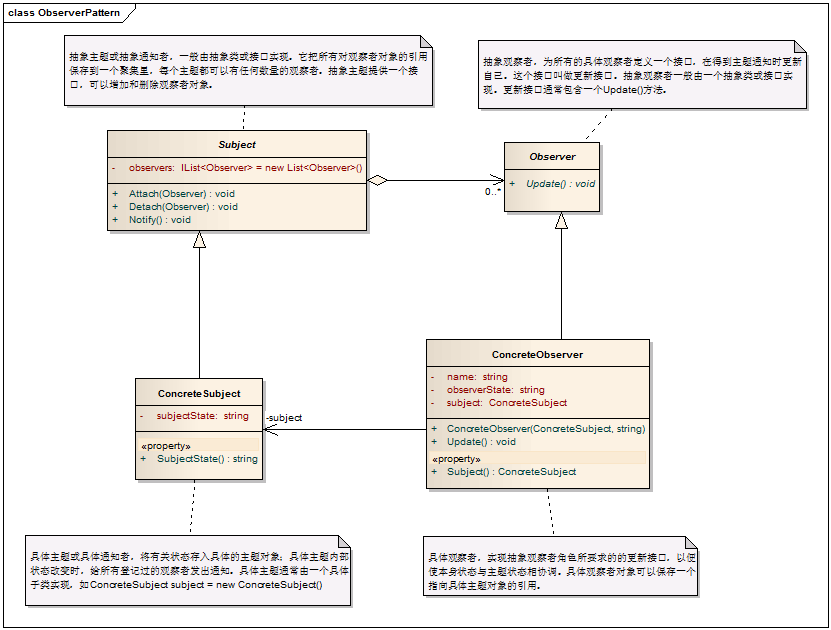
\includegraphics[width=.9\linewidth]{./pic/observer.png}
\end{center}
\item Unity3d教程:设计模式之观察模式
\item 观察者模式的代码
\begin{minted}[linenos=true]{csharp}
// 抽象主题类
public abstract class Subject {
    private IList observers = new List();
	// 增加观察者
    public void Attach(Observer observer) {
        observers.Add(observer);
    }
	// 移除观察者
    public void Detach(Observer observer) {
        observers.Remove(observer);
    }
	// 向观察者(们)发出通知
    public void Notify() {
        foreach (Observer o in observers) {
            o.Update();
        }
    }
}

// 抽象观察者类,为所有具体观察者定义一个接口,在得到通知时更新自己
public abstract class Observer {
    public abstract void Update();
}

// 具体观察者或具体通知者,将有关状态存入具体观察者对象;在具体主题的内部状态改变时,给所有登记过的观察者发出通知。具体主题角色通常用一个具体子类实现。
public class ConcreteSubject : Subject {
    private string subjectState;
	// 具体观察者的状态
    public string SubjectState {
        get { return subjectState; }
        set { subjectState = value; }
    }
}

// 具体观察者,实现抽象观察者角色所要求的更新接口,已是本身状态与主题状态相协调
public class ConcreteObserver : Observer {
    private string observerState;
    private string name;
    private ConcreteSubject subject;
    
	// 具体观察者用一个具体主题来实现
    public ConcreteSubject Subject {
        get { return subject; }
        set { subject = value; }
    }
    public ConcreteObserver(ConcreteSubject subject, string name) {
        this.subject = subject;
        this.name = name;
    }
	// 实现抽象观察者中的更新操作
    public override void Update() {
        observerState = subject.SubjectState;
        Console.WriteLine("The observer's state of {0} is {1}", name, observerState);
    }
}
\end{minted}
\item 客户端代码
\begin{minted}[linenos=true]{csharp}
class Program {
    static void Main(string[] args) {
	// 具体主题角色通常用具体自来来实现
        ConcreteSubject subject = new ConcreteSubject();
        subject.Attach(new ConcreteObserver(subject, "Observer A"));
        subject.Attach(new ConcreteObserver(subject, "Observer B"));
        subject.Attach(new ConcreteObserver(subject, "Observer C"));
        subject.SubjectState = "Ready";
        subject.Notify();
        Console.Read();
    }
}
\end{minted}
\item 运行结果
\item Unity3d教程:设计模式之观察模式
\end{itemize}
\subsubsection{模式总结}
\label{sec:orgdb1b889}
\begin{enumerate}
\item 优点
\label{sec:orgbdf600a}
观察者模式解除了主题和具体观察者的耦合,让耦合的双方都依赖于抽象,而不是依赖具体。从而使得各自的变化都不会影响另一边的变化。
\item 缺点
\label{sec:org696cd50}
\begin{itemize}
\item 依赖关系并未完全解除,抽象通知者依旧依赖抽象的观察者。
\end{itemize}
\item 适用场景
\label{sec:org875caed}
\begin{itemize}
\item 当一个对象的改变需要给变其它对象时,而且它不知道具体有多少个对象有待改变时。
\item 一个抽象某型有两个方面,当其中一个方面依赖于另一个方面,这时用观察者模式可以将这两者封装在独立的对象中使它们各自独立地改变和复用。
\item 
\end{itemize}
\end{enumerate}

\subsection{C\#设计模式学习笔记之建造者模式(Builder)}
\label{sec:orgfebcb63}
\begin{itemize}
\item \url{http://www.58kaifa.com/article/177}
\item 建造者模式(Builder)概述:
\item 在构造一个对象的时候,往往有很多复杂的过程和次序,例如建造一个机器人,那要先造头,还是要先造身子,这就关乎到一个制造工序的问题。其实建造者模式(Builder)和工厂模式很接近的,但是建造模式提供了一个更加细粒度的对象的建造过程。
\item 定义:
\item 建造者模式(Builder)将复杂的结构与其表示分离,使得同样的构建过程可以创建不同的表示。
\item 原型模式应用:
\item 在软件系统中,有时候面临一个复杂对象的创建工作,该对象通常由各个部分子对象用一定的算法构成,或者按一定的步骤组合而成;这些算法和步骤是稳定的,而构成这个对象的子对象却经常由于需求的变化而不断变化。
\item 假设要组装一台电脑,它的组装过程基本是不变的,都可以由主板、CPU、内存等按照某个稳定方式组合而成。然而主板、cpu、内存等零件本身是可能多变的。将内存等这种易变的零件与电脑的其他部件分离,实现解耦合,则可以轻松实现电脑不断升级。
\item 建造模式结构图:
\item 建造模式参与者:
\item Builder(抽象建造者):给出一个抽象接口,以规范产品对象的各个组成成分的建造。这个接口规定要实现复杂对象的哪些部分的创建,并不涉及具体的对象部件的创建。
\item ConcreteBuilder(建造者):实现Builder接口,针对不同的商业逻辑,具体化负责对象的各部分的创建,在建造过程完成后,提供产品的实例。
\item Director(导演类):调用具体建造者来创建复杂对象的各个部分,在导演类中不急具体产品的信息,只复杂保证对象各个部分完整创建或按某种顺序创建。
\item Product(产品类):
\item 表示被构造的复杂对象。ConcreteBuilder创建该产品的内部表示并定义它的装配过程
\item 包含定义组成部件的类,包括将这些部件装配成最终产品的接口
\item 在建造者模式中,Director规定了创建一个对象所需要的步骤和次序,Builder则提供了一些列完成这些步骤的方法,ConcreteBuilder 给出了这些方法的具体实现,是对象的直接创建者。
\item 建造者模式结构实现:
\begin{minted}[linenos=true]{csharp}
// 产品类
public class Product {
    private List<string> _parts = new List<string>();
    public void Add(string part) {
        _parts.Add(part);
    }
    public void Show() {
        Console.WriteLine("Product Parts");
        foreach (string part in _parts) {
            Console.WriteLine(part);
        }
    }
}
 
// 抽象建造者类
public abstract class Builder {
    public abstract void BuildPartA();
    public abstract void BuildPartB();
    public abstract Product GetResult();
}
// 建造者1
public class ConcreteBuilder1 : Builder {
    private Product _product = new Product();
    public override void BuildPartA() {
        _product.Add("PartA");
    }
    public override void BuildPartB() {
        _product.Add("PartB");
    }
    public override Product GetResult() {
        return _product;
    }
}
// 建造者2
public class ConcreteBuilder2 : Builder {
    private Product _product = new Product();
    public override void BuildPartA() {
        _product.Add("Partx");
    }
    public override void BuildPartB() {
        _product.Add("PartY");
    }
    public override Product GetResult() {
        return _product;
    }
 
}
// 导演类
public class Director {
    public void Construct(Builder builder) {
        builder.BuildPartA();
        builder.BuildPartB();
    }
}
// 客户端
class Client {
    static void Main(string[] args) {
        Director director = new Director();
        Builder b1 = new ConcreteBuilder1();
        Builder b2 = new ConcreteBuilder2();

        director.Construct(b1);
        Product p1 = b1.GetResult();
        p1.Show();
 
        director.Construct(b2);
        Product p2 = b2.GetResult();
        p2.Show();
 
    }
}
\end{minted}
\item 建造者模式实例
\item 建造小人,要求:小人必须包括,头,身体,手和脚。现在系统要包括的分为胖子和瘦子:
\begin{minted}[linenos=true]{csharp}
// 产品类
class Product {
    private List<string> _part = new List<string>();
    public void Add(string part) {
        _part.Add(part);
    }
    public void Show() {
        foreach (string part in _part) {
            Console.WriteLine(part);
        }
    }
}
// 抽象建造者
public abstract class Builder {
    public abstract void BuildHead();
    public abstract void BuildBody();
    public abstract void BuildHand();
    public abstract void BuildFeet();
    public abstract Product GetResult();
}
// 胖子建造
public class FatPBuilder : Builder {
    private Product _product;
    public override void BuildHead() {
        _product.Add("胖子头");
    }
    public override void BuildBody() {
        _product.Add("胖子身体");
    }
    public override void BuildHand() {
        _product.Add("胖子手");
    }
    public override void BuildFeet() {
        _product.Add("胖子脚");
    }
    public override Product GetResult() {
        return _product;
    }
}
// 瘦子建造
public class ThinPBuilder : Builder {
    private Product _product;
    public override void BuildHead() {
        _product.Add("瘦子头");
    }
    public override void BuildBody() {
        _product.Add("瘦子身体");
    }
    public override void BuildHand() {
        _product.Add("瘦子手");
    }
    public override void BuildFeet() {
        _product.Add("瘦子脚");
    }
    public override Product GetResult() {
        return _product;
    }
}
// 导演类
public class Director {
    public void Construct(Builder builder) {
        builder.BuildHead();
        builder.BuildBody();
        builder.BuildHand();
        builder.BuildFeet();
    }
}
// 客户端类
public class Client {
    static void Main(string[] args) {
        Director _director = new Director();
        Builder b1 = new FatPBuilder();
        Builder b2 = new ThinPBuilder();
        _director.Construct(b1);
        Product p1 = b1.GetResult();
        p1.Show();
    }
}
\end{minted}
\item 汽车生产 
\begin{minted}[linenos=true]{csharp}
// 车辆产品类
public class Vehicle {
    private string _vehicleType;
    private Dictionary<string, string> _parts = new Dictionary<string, string>();
 
    public Vehicle(string vehicleType) {
        this._vehicleType = vehicleType;
    }
 
    public string this[string key] {
        get { return _parts[key]; }
        set { _parts[key] = value; }
    }
 
    public void Show() {
        Console.WriteLine("\n----------------------");
        Console.WriteLine("Vehicle Type:{}",_vehicleType);
        Console.WriteLine("Frame:{0}",_parts["frame"]);
        Console.WriteLine("Engine:{0}", _parts["engine"]);
        Console.WriteLine("#Wheels{0}",_parts["wheels"]);
        Console.WriteLine("#Doors:{0}",_parts["doors"]);
    }
}

// 汽车制作抽象类
public abstract class VehicleBuilder {
    protected Vehicle vehicle;
    public Vehicle Vechicle {
        get { return Vechicle; }
    }
    public abstract void BuildFrame();
    public abstract void BuildEngine();
    public abstract void BuildWheels();
    public abstract void BuildDoors();
}

// 摩托车制作类
public class MotorCycleBuilder : VehicleBuilder {
    public MotorCycleBuilder() {
        vehicle = new Vehicle("MotorCycle");
    }
    public override void BuildFrame() {
        vehicle["Frame"] = "MotorCycle Frame";
    }
    public override void BuildEngine() {
        vehicle["engine"] = "500 cc";
    }
    public override void BuildWheels() {
        vehicle["wheels"] = "2";
    }
    public override void BuildDoors() {
        vehicle["doors"] = "0";
    }
}

// 踏板车类制作类
public class ScooterBuilder : VehicleBuilder {
    public ScooterBuilder() {
        vehicle = new Vehicle("Scooter");
    }
    public override void BuildFrame() {
        vehicle["Frame"] = "Scooter Frame";
    }
    public override void BuildEngine() {
        vehicle["engine"] = "50 cc";
    }
    public override void BuildWheels() {
        vehicle["wheels"] = "2";
    }
    public override void BuildDoors() {
        vehicle["doors"] = "0";
    }
}

// 商店类
public class Shop {
    public void Construct(VehicleBuilder vb) {
        vb.BuildFrame();
        vb.BuildEngine();
        vb.BuildWheels();
        vb.BuildDoors();
    }
}

// 客户端类
class Client {
    static void Main(string[] args) {
        VehicleBuilder builder;
        Shop shop = new Shop();
 
        builder = new ScooterBuilder();
        shop.Construct(builder);
        builder.Vechicle.Show();
 
        builder = new MotorCycleBuilder();
        shop.Construct(builder);
        builder.Vechicle.Show();
    }
}
\end{minted}
\end{itemize}
建造者模式应用分析
\begin{itemize}
\item 需要生成的产品对象有复杂的内部结构
\item 需要生成的产品对象的属性相互依赖,建造者模式可以强迫生成顺序
\item 在对象创建过程会使用到系统中的一些其他对象,这些对象在产品对象的创建过程中不易得到
\item 建造者模式特点:
\item 建造者模式的使用使得产品的内部表对象可以独立地变化。使用建造者模式可以使客户不必知道产品内部组成的细节
\item 每一个builder都相对独立,而与其他builder无关
\item 可使对构造过程更加精细控制
\item 将构建代码和表示代码分开
\item 建造者模式的缺点在于难于应付分步步骤构造算法的需求变动。
\item ConcreteBuilder),用来实现抽象制造类中的操作,并进行现象内容的操作。(可定义多个,继承抽象制造者(Builder)类)
\item Director),用来实现操作的流程。
\item ConcreteBuilder),在ConcreteBuilder中我们根据Builder里定义操作来进行组装,在这里我们可以在操作中定义我们CPU使用什么型号,主板用什么型号,内存用的时多打内存等等。
\end{itemize}


\subsection{C\#设计模式学习笔记之工厂设计模式}
\label{sec:org7441f38}
\begin{itemize}
\item \url{http://www.58kaifa.com/article/171}
\item 模式概述:
\item 工厂方法(Factory Method)模式又成为工厂模式,属于类的创建型模式。在工厂方法模式中,父类负责定义创建对象的公共接口,子类负责生产具体的对象,这样做的目的是将类的实例化操作延迟到子类中完成,即由子类决定究竟应该实例哪个类。
\item 定义:
\item 工厂方法模式定义一个永远创建对象的接口,让子类决定实例化哪一个类。工厂方法模式是以一个类的实例化延迟到其子类。
\item Factory Method 模式用于在不指定待创建对象的具体类的情况下创建对象。
\item Factory Method 模式的主要意图是隐藏对象创建的负责性。Client通常不指定要创建的具体类,Client将面向接口或抽象类进行编码,让Factory类负责创建具体的类型。通常Factory类有一个返回抽象类或接口的静态方法。Client通常提供某种信息让Factory类使用提供的信息来确定创建并返回哪个子类。
\item 将创建子类的责任抽象出来的好处是允许Client完成无需考虑依赖类是如何创建。这遵守依赖倒置原则(DIP)。Factory Method 模式另外一个好处是把负责对象创建的代码集中起来,如果需要修改对象生产方式,可以轻松定位并跟新,而不会影响到依赖它的代码。
\item 在面向对象编程中,一般方法是用一个new操作符产生一个对象的实例。但是在一些情况下,用new操作符直接生产对象会带来一些问题。首先,要使用new运算符创建一个对象必须清楚所要创建的对象的类信息,包括类名、构造函数等,而又时并不现实。其次许多类型的对象创建需要一系列的步骤,可能需要计算或取得对系那个的初始设置,选择生产那个对象实例,或在需要的对象之前必须生产一些辅助功能的对象。在这些情况下,新对象的创建就是一个过程,而不是一个简单的操作。
\item 工厂方法模式结构:
\item 工厂模式参与者:
\item Product:抽象的产品角色,定义工厂方法所创建的对象接口
\item ConcreteProduct:具体Product角色,实现Product接口
\item Factory:抽象的工厂角色,声明工厂方法,返回一个Product类型的对象
\item Factory可以定义一个工厂方法的默认实现,返回一个默认的ConcreteProduct对象。可以调用工厂方法创建一个Product对象。
\item ConcreteFactory:具体的工厂角色,创建具体Product的子工厂,重写工厂方法以返回一个ConcreteProduct实例。
\item 工厂方法模式结构实现:
\begin{minted}[linenos=true]{csharp}
// 工厂模式结构实现
// 抽象产品类
public class Product {
}
// 具体产品类A
public class ConcreteProductA : Product {
}
// 具体产品类B
public class ConcreteProductB : Product {
}
// 抽象工厂类
public abstract class Factory {
    public abstract Product CreateProduct();
}
// 具体工厂A
public class ConcreteFactoryA : Factory {
    public override Product CreateProduct() {
        return new ConcreteProductA();
    }
}
// 具体工厂B
public class ConcreteFactoryB : Factory {
    public override Product CreateProduct() {
        return new ConcreteProductB();
        throw new NotImplementedException();
    }
}
///客户端类
public class Client {
    static void Main(string[] args) {
        Factory[] factories = new Factory[2];
        factories[0] = new ConcreteFactoryA();
        factories[1] = new ConcreteFactoryB();

        foreach (Factory factory in factories) {
            Product product = factory.CreateProduct();
            Console.WriteLine("Created{0}",product.GetType().Name);
        }
    }
}
//  工厂模式应用1:扩展刷卡处理
//  在简单工厂模式应用中我们谢了刷卡处理的应用,但是突然公司要添加新的卡种,
//  就可以很使用工厂模式来做,只要增加卡的处理类和生产卡处理类的工厂。
    
//  抽象产品类
abstract class BankCardHandle {
    public abstract void HandleProcess();
}
// 具体产品类VISA,继承抽象产品类
class VisaHandle : BankCardHandle {
    public override void HandleProcess() {
        Console.WriteLine("Visa卡处理中..");
    }
}
// 具体产品类Master,继承抽象产品类
class MasterCardHandle : BankCardHandle {
    public override void HandleProcess() {
        Console.WriteLine("Master卡处理中..");
    }
}
// 抽象工厂类
public abstract class HandleFactory {
    public abstract BankCardHandle CreateBankCardHandle();
}
// 具体工厂类,继承抽象工厂类
public class VisaFactory:HandleFactory {
    public override BankCardHandle CreateBackCardHandle() {
        return new VisaHandle();
    }
}
// 具体工厂类,继承抽象工厂类
public class MasterFactory:HandleFactory {
    public override BankCardHandle CreateBackCarHandle() {
        return new BankCardHandle();
    }
}
// 客户端调用
class Client {
    public static void Main(string[] args) {
        //实例化工厂
        HandleFactory visaFacotry = new VisaFactory();
        HandleFactory masterFactory = new MasterFactory();
        //创建卡类
        BankCardHandle vf = visaFacotry.CreateBackCarHandle();
        BankCardHandle mf = masterFactory.CreateBackCarHandle();
        //新添加的卡种
        HandleFactory unionFactory = new UnionPayCardFactory();
        BankCardHandle nf = unionFactory.CreateBackCarHandle();
    }
}
// 新添加的卡的特性
public class UnionPayCardHandle : BankCardHandle {
    public override void HandleProcess() {
        Console.WriteLine("银联卡处理中..");
    }
}
// 新添加的卡的工厂
public class UnionPayCardFactory : HandleFactory {
    public override BankCardHandle CreateBackCarHandle() {
        return new UnionPayCardHandle();
    }
}
\end{minted}
\item 工厂模式应用:
\item 扩展刷卡应用
\begin{minted}[linenos=true]{csharp}
// KFC生产:
// 应用实例:KFC生产模式
///抽象产品类
public abstract class KFCFood {
    public abstract void Display();
}
// 具体产品类 鸡腿
public class Chicken : KFCFood {
    public override void Display() {
        Console.WriteLine("鸡腿+1");
    }
}
// 具体产品类鸡翅
public class Wings : KFCFood {
    public override void Display() {
        Console.WriteLine("鸡翅+1");
    }
}
// 抽象工厂类
public abstract/interface class KFCFactory {
    public abstract KFCFood CreateFood();
 
}
// 具体工厂类 鸡腿工厂
public class ChikenFactory:KFCFactory {
    public override KFCFood CreateFood() {
        return new Chicken();
    }
}
// 具体工厂类 鸡翅工厂
public class WingsFactory:KFCFactory {
    public override KFCFood CreateFood() {
        return new Wings();
    }
}
// 客户端类
public class Client {
    public static void Main(string[] args) {
        //创建鸡腿和鸡翅工厂
        KFCFactory chichen = new KFCFactory();
        KFCFactory wings = new KFCFactory();
        //生产鸡腿
        KFCFood food1  = chichen.CreateFood();
        food1.Display();
 
        KFCFood food2  = chichen.CreateFood();
        food1.Display();
        //生产鸡翅
        KFCFood food3 = wings.CreateFood();
        food3.Display();
    }
}
\end{minted}
\item 工厂模式方法应用分析:
\item 1、工厂模式使用情形:
\item 当一个类不知道它所必须创建的对象的类信息的时候
\item 当一个类希望由它来指定它所创建的对象的时候
\item 当类将创建对象的职责委托给多个辅助子类中的某一个,希望将哪一个辅助之类时代理者这以信息局部化的时候
\item 2、工厂模式特点
\item 使用工厂方法在一个类的内部创建对象通常比直接创建对象更灵活
\item 工厂方法模式通过面向对象的手法,将所要创建的具体对象的创建工作延迟到子类,从而提供了一种扩展的策略,较好的解决了紧耦合的关系
\item 工厂方法模式遵守依赖倒置原则(DIP);
\item 总结:
\item 相对于简单工厂模式而言,工厂方法模式的核心是一个抽象工厂类,而简单工厂模式把核心放在一个具体工厂类上。在工厂模式中,子工厂与产品往往具有平行的的等级结构,他们之间一一对应。
\item 就上一节玩具工厂来说,我们知道有一台机器可以设定多个模式,那么可以多买几台机器,每台机器的设定不一样,比如,这一是生产小熊用的,另一台是生产汽车用的,当我们需要那种玩具的时候就用相对的机器进行生产。可以工厂模式就是多个简单工厂模式的综合。
\end{itemize}
\section{Camera 相关}
\label{sec:org1b8f1b3}
\subsection{Camera Shake in Unity}
\label{sec:org4bceb15}
\begin{itemize}
\item \url{http://www.voidcn.com/article/p-yfmjbkxr-pu.html}
\begin{minted}[linenos=true]{javascript}
var originPosition:Vector3;
var originRotation:Quaternion;
var shake_decay: float;
var shake_intensity: float;;
function OnGUI () {
    if (GUI.Button (Rect (20,40,80,20), "Shake")) {
        Shake();
    }
}
function Update(){
    if(shake_intensity > 0){
        transform.position = originPosition + Random.insideUnitSphere * shake_intensity;
        transform.rotation =  Quaternion(
                    originRotation.x + Random.Range(-shake_intensity,shake_intensity)*.2,
                    originRotation.y + Random.Range(-shake_intensity,shake_intensity)*.2,
                    originRotation.z + Random.Range(-shake_intensity,shake_intensity)*.2,
                    originRotation.w + Random.Range(-shake_intensity,shake_intensity)*.2);
        shake_intensity -= shake_decay;
    }
}
function Shake(){
    originPosition = transform.position;
    originRotation = transform.rotation;
    shake_intensity = .3;
    shake_decay = 0.002;
}
\end{minted}
\end{itemize}

\subsection{Unity中做放大镜 效果}
\label{sec:org8982ca3}
\begin{itemize}
\item \url{http://www.voidcn.com/article/p-qyltseeo-ry.html}
\item 其实和 小地图都差不多了。  还是要借助 另一个相机
\item 目的: 这篇文章的主要目的是  要给你一个想法  如何做放大境效果 。
\item 在unity中可以简单的实现放大镜效果啊 . 那么现在就来一步一步实现这个:
\item 创建一个摄像机对象,设置 projection 类型为 perspective 或者 orthographic.
\item 设置相机的 orthographicSize 或者 fieldOfView   (依赖于相机的 projection 类型 ).
\item 设置其 pixelrect  . 例如如果您想要在你鼠标位置显示放大境  和其大小是 100 x 100 , 然后设置pixelrect 为 :
\end{itemize}
\begin{minted}[linenos=true]{csharp}
 magnifyCamera.pixelRect = new Rect (Input.mousePosition.x – 100f / 2.0f, Input.mousePosition.y – 100f / 2.0f, 100f, 100f);
\end{minted}
\begin{itemize}
\item 设置相机的位置。  例如 如果你想在 你的鼠标位置显示放大镜效果  ,那么设置相机的位置为 mousePosition世界点。
\item 下面的 C\# 脚本将创建一个  MagnifyGlass,并将它移动到 mousePosition位置 。
\item MagnifyGlass 脚本:   添加到一个空的游戏对象。

\begin{minted}[linenos=true]{csharp}
using UnityEngine;
using System.Collections;
 
public class MagnifyGlass : MonoBehaviour {
    private Camera magnifyCamera;
    private GameObject magnifyBorders;
    private LineRenderer LeftBorder, RightBorder, TopBorder, BottomBorder; // Reference for lines of magnify glass borders
    private float MGOX, MG0Y; // Magnify Glass Origin X and Y position
    private float MGWidth = Screen.width/5f, MGHeight = Screen.width/5f; // Magnify glass width and height
    private Vector3 mousePos;
 
    void Start () {
        createMagnifyGlass ();
    }
    
    void Update () {
// Following lines set the camera's pixelRect and camera position at mouse position
        magnifyCamera.pixelRect = new Rect (Input.mousePosition.x - MGWidth / 2.0f, Input.mousePosition.y - MGHeight / 2.0f, MGWidth, MGHeight);
        mousePos = getWorldPosition (Input.mousePosition);
        magnifyCamera.transform.position = mousePos;
        mousePos.z = 0;
        magnifyBorders.transform.position = mousePos;
    }
 
// Following method creates MagnifyGlass
    private void createMagnifyGlass() {
        GameObject camera = new GameObject("MagnifyCamera");
        MGOX = Screen.width / 2f - MGWidth/2f;
        MG0Y = Screen.height / 2f - MGHeight/2f;
        magnifyCamera = camera.AddComponent<Camera>();
        magnifyCamera.pixelRect = new Rect(MGOX, MG0Y, MGWidth, MGHeight);
        magnifyCamera.transform.position = new Vector3(0,0,0);
        if (Camera.main.isOrthoGraphic) {
            magnifyCamera.orthographic = true;
            magnifyCamera.orthographicSize = Camera.main.orthographicSize / 5.0f;//+ 1.0f;
            createBordersForMagniyGlass ();
        } else {
            magnifyCamera.orthographic = false;
            magnifyCamera.fieldOfView = Camera.main.fieldOfView / 10.0f;//3.0f;
        }
    }
 
// Following method sets border of MagnifyGlass
private void createBordersForMagniyGlass() {
magnifyBorders = new GameObject ();
LeftBorder = getLine ();
LeftBorder.SetVertexCount(2);
LeftBorder.SetPosition(0,
                       new Vector3(getWorldPosition(new Vector3(MGOX,MG0Y,0)).x,
                                   getWorldPosition(new Vector3(MGOX,MG0Y,0)).y-0.1f,
                                   -1));
LeftBorder.SetPosition(1,
                       new Vector3(getWorldPosition(new Vector3(MGOX,MG0Y+MGHeight,0)).x,
                               getWorldPosition(new Vector3(MGOX,MG0Y+MGHeight,0)).y+0.1f,
                                   -1));
LeftBorder.transform.parent = magnifyBorders.transform;
TopBorder = getLine ();
TopBorder.SetVertexCount(2);
TopBorder.SetPosition(0,
                      new Vector3(getWorldPosition(new Vector3(MGOX,MG0Y+MGHeight,0)).x,
                                  getWorldPosition(new Vector3(MGOX,MG0Y+MGHeight,0)).y,
                                  -1));
TopBorder.SetPosition(1,
                  new Vector3(getWorldPosition(new Vector3(MGOX+MGWidth,MG0Y+MGHeight,0)).x,
                          getWorldPosition(new Vector3(MGOX+MGWidth,MG0Y+MGHeight,0)).y,
                          -1));
TopBorder.transform.parent = magnifyBorders.transform;
RightBorder = getLine ();
RightBorder.SetVertexCount(2);
RightBorder.SetPosition(0,
                new Vector3(getWorldPosition(new Vector3(MGOX+MGWidth,MG0Y+MGWidth,0)).x,
                       getWorldPosition(new Vector3(MGOX+MGWidth,MG0Y+MGWidth,0)).y+0.1f,
                                    -1));
RightBorder.SetPosition(1,
                      new Vector3(getWorldPosition(new Vector3(MGOX+MGWidth,MG0Y,0)).x,
                                getWorldPosition(new Vector3(MGOX+MGWidth,MG0Y,0)).y-0.1f,
                                    -1));
RightBorder.transform.parent = magnifyBorders.transform;
BottomBorder = getLine ();
BottomBorder.SetVertexCount(2);
BottomBorder.SetPosition(0,
                         new Vector3(getWorldPosition(new Vector3(MGOX+MGWidth,MG0Y,0)).x,
                                     getWorldPosition(new Vector3(MGOX+MGWidth,MG0Y,0)).y,
                                     -1));
BottomBorder.SetPosition(1,
                         new Vector3(getWorldPosition(new Vector3(MGOX,MG0Y,0)).x,
                                     getWorldPosition(new Vector3(MGOX,MG0Y,0)).y,
                                     -1));
BottomBorder.transform.parent = magnifyBorders.transform;
}

// Following method creates new line for MagnifyGlass's border
    private LineRenderer getLine() {
        LineRenderer line = new GameObject("Line").AddComponent<LineRenderer>();
        line.material = new Material(Shader.Find("Diffuse"));
        line.SetVertexCount(2);
        line.SetWidth(0.2f, 0.2f);
        line.SetColors(Color.black,  Color.black);
        line.useWorldSpace = false;
        return line;
    }
    private void setLine(LineRenderer line) {
        line.material = new Material(Shader.Find("Diffuse"));
        line.SetVertexCount(2);
        line.SetWidth(0.2f, 0.2f);
        line.SetColors(Color.black, Color.black);
        line.useWorldSpace = false;
    }
 
// Following method calculates world's point from screen point as per camera's projection type
    public Vector3 getWorldPosition(Vector3 screenPos) {
        Vector3 worldPos;
        if(Camera.main.isOrthoGraphic) {
            worldPos = Camera.main.ScreenToWorldPoint (screenPos);
            worldPos.z = Camera.main.transform.position.z;
        } else {
            worldPos = Camera.main.ScreenToWorldPoint (new Vector3 (screenPos.x, screenPos.y, Camera.main.transform.position.z));
            worldPos.x *= -1;
            worldPos.y *= -1;
        }
        return worldPos;
    }
}
\end{minted}
\end{itemize}

\subsection{Unity 3D-- 摄像机Clear Flags和Culling Mask属性用途详解}
\label{sec:org1aba5fb}
\begin{itemize}
\item \url{http://www.voidcn.com/article/p-pwbltogg-pu.html}
\end{itemize}

\subsection{[Unity基础]对Camera组件属性的一些理解}
\label{sec:org7667928}
\begin{itemize}
\item \url{http://www.voidcn.com/article/p-gtfuejmb-uz.html}
\end{itemize}

\subsection{Unity的camera组件}
\label{sec:orgb075975}
\begin{itemize}
\item \url{http://www.voidcn.com/article/p-mcxkifby-cb.html}
\end{itemize}

\subsection{unity Camera 属性详解}
\label{sec:org17d1316}
\begin{itemize}
\item \url{http://www.voidcn.com/article/p-enwwkrfr-hh.html}
\end{itemize}

\section{Lights Lighting related}
\label{sec:org6c0c8d2}
\subsection{渲染管线中的Rendering Path}
\label{sec:org5347c8e}
\begin{itemize}
\item \url{https://yq.aliyun.com/articles/49406}
\item Unity3D中,目前保存了4种Rending Path.
\begin{itemize}
\item 1、Deferred Shading Rendering Path(延迟渲染)
\item 2、Forward Rendering Path(前向渲染)
\item 3、Lagacy Deferred Lighting Rendering Path(延迟光照)
\item 4、Vertex Lit Rendering Path(顶点光照)
\end{itemize}
\end{itemize}

\subsubsection{Forward Rendering Path(前向渲染)}
\label{sec:orgba813e2}
\begin{itemize}
\item 官方文档:\url{http://docs.unity3d.com/Manual/RenderTech-ForwardRendering.html}
\item 传统的前向着色渲染方式是一种简单粗暴的方式。就是一次性将一个物体绘制完再绘制下一个。光照计算也是如此。前向着色最主要的问题就是光照问题。当光源过多的时候,就需要进行处理。 而Unity3D在光源处理方面,也结合了像素光照(per-pixel lighting) ,顶点光照(per-vertex lighting),球谐光照(Spherical Harmonics lighting)等多种方案,其复杂程度可见一斑。
\end{itemize}
\begin{enumerate}
\item Unity3D中前向渲染的光源策略
\label{sec:orgfe94154}
\begin{itemize}
\item 前向着色渲染由于效率和寄存器限制等原因。不可能老老实实地去处理所有的光源。因此,需要根据光源的远近,范围,重要程度等因子决定计算方式。
\begin{itemize}
\item 1、如果一个光源的RenderMode没有设置为重要(Important),那么它将永远是逐顶点或者球谐光照计算方式。
\item 2、最亮的(Brightest)方向光源会做为逐像素光照计算。
\item 3、如果一个光源的RenderMode设置为重要(Important),那么它将会采用逐像素光照计算方式
\item 4、如果上面的结果中的用于逐像素计算的光源数目小于了Project Settings->Quality面板中的Pixel Light Count值。 为了减少亮度误差,有一些光源会被当作像素光源计算(PS:非像素光源无法完全计算阴影关系。会导致场景偏亮)。
\item 5、Unity3D对顶点光照,像素光照做了最大限制。 分别为4个。而场景中不可能只有这么多光源。因此,使用了一个优先级判定。
\end{itemize}

\begin{center}
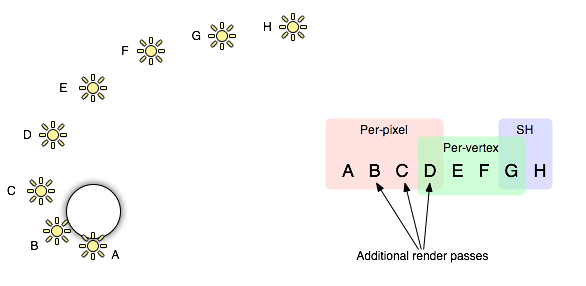
\includegraphics[width=.9\linewidth]{./pic/lighting.jpg}
\end{center}
\begin{itemize}
\item 左:光源位置图
\item 右:光源分配图
\end{itemize}
\item 从图中我们可以看到。 D参与了像素和顶点光照。 G参与了顶点光照和球谐光照。 这样的处理应该是为了做一个光照信息的平滑衔接,不至于变得很突兀。
\end{itemize}
\item Unity3D中前向渲染的光照的计算过程
\label{sec:orgd91a7fc}
\begin{itemize}
\item 前向渲染中,光照计算被分成了多个PASS。通常它们由1*FarwardBase Pass + N*FarwardAdd Pass组成。可以看出,光源的数目在前向渲染管线中是一个致命的效率杀手。
\begin{itemize}
\item 1、Base Pass 提交一个逐像素方向光和所有的逐顶点光照和球谐光照。
\item 2、Additional Pass 提交一个逐像素的光照计算。 如果一个物体受更多的光源影响。那么就会有许多PASS需要进行绘制。
\begin{itemize}
\item 注:在Shader中。可以指定FarwardBase来关掉Additional 功能。
\item 注:在前向渲染中,只能有一个方向光实时阴影。
\end{itemize}
\end{itemize}
\end{itemize}
\item Unity3D中的球谐光照
\label{sec:org079c217}
\begin{itemize}
\item 球谐光照是一个CPU光照算法。它可以处理大规模的光源信息,非常适合一些很小的动态点光源。但是它存在以下几个问题。
\begin{itemize}
\item 1、球谐光照是基于物体顶点的算法,并非像素级。这就意味着它不能使用一些像素级的效果增强手段。比如法线贴图。
\item 2、基于效率的考虑,球谐光照的更新频率非常低。如果光源移动过快,就会穿邦。
\item 3、球谐光照是基于全局空间的计算,当一个面离点光源或者聚光灯很近时,效果是错的。
\end{itemize}
\end{itemize}
\end{enumerate}

\subsubsection{Deferred Shading Rendering Path(延迟渲染)}
\label{sec:org1e7df98}
\begin{itemize}
\item 官方文档:\url{http://docs.unity3d.com/Manual/RenderTech-DeferredShading.html}
\end{itemize}
\begin{enumerate}
\item 延迟渲染技术简介
\label{sec:org7192fd0}
\begin{itemize}
\item 延迟渲染技术已经是一个成熟且稳定的技术。已经广泛用于各种商业引擎中。它主要解决的是当光源数目过多时带来的复杂光照计算的开销。 在传统前向渲染中,假设一个场景中有M个物体,N个光源。 那么理论上进行的光照计算次数为 M*N。 而DS管线可以使其变为M+N。
\item 但是DS管线并非万能的。有以下情况需要注意
\end{itemize}
\item 延迟渲染技术缺陷
\label{sec:org3bb3835}
\begin{itemize}
\item 1、DS需要多渲染目标(MRT)的支持、深度纹理、双面模板缓存。
\begin{itemize}
\item 这个特性,需要显卡支持SM3.0的API。2006年以后的PC显卡应该不成问题。比如GeForce 8xxxx,AMD Radeon X2400,Intel G45以后的显卡。
\end{itemize}
\item 2、DS管线会消耗更多的显存,用于缓存G-Buffer。同时,会要求显卡拥有更大的位宽(bit counts)。
\begin{itemize}
\item 在手机上目前(2016年)还不实现。
\end{itemize}
\item 3、DS管线无法处理半透明物体。
\begin{itemize}
\item 半透明物体需要退回到传统前向渲染中进行
\end{itemize}
\item 4、硬件抗锯齿(MSAA)无法使用。
\begin{itemize}
\item 只能使用一些后期算法,如FXAA等。
\end{itemize}
\item 5、这句话中的内容目前未测试,故无法准确体会其中的意思:There is also no support for the Mesh Renderer’s Receive Shadows flag and culling masks are only supported in a limited way. You can only use up to four culling masks. That is, your culling layer mask must at least contain all layers minus four arbitrary layers, so 28 of the 32 layers must be set. Otherwise you will get graphical artefacts.
\end{itemize}
\item 延迟渲染技术在Unity3D中的实现方案
\label{sec:org5c22ff8}
\begin{itemize}
\item Unity3D中,延迟渲染管线为分两个阶段进行。G-Buffer阶段和光照计算(Lighting)阶段。
\end{itemize}
\item G-Buffer阶段
\label{sec:org7c018bc}
\begin{itemize}
\item Unity3D渲染所有的非透明对象到各个RT中,RT的内容分布见 G-Buffer内容。Unity3D将各个RT做成了全局变量,方面Shader中进行操作。像这样:CameraGBufferTexture0 .. CameraGBufferTexture3
\end{itemize}
\item 光照计算阶段
\label{sec:org7c64973}
\begin{itemize}
\item 这个阶段的主要目的就是根据G-Buffer的内容进行光照计算。由于是屏幕空间的计算,显然要比之前的前向渲染来得容易得多。
\begin{itemize}
\item 注:实时阴影的计算是在光照计算之前的。 DS管线并不能减少实时阴影的开销。应该怎么整还得怎么整。最后,每个物体受到的实时阴影的影响会叠加到RT3中。一些特殊的爆光效果,Lightmap光影贴图效果等都会进入RT3。 参见G-Buffer内容
\end{itemize}
\item G-Buffer内容
\begin{itemize}
\item •RT0, ARGB32 format: Diffuse color (RGB), occlusion (A).
\item •RT1, ARGB32 format: Specular color (RGB), roughness (A).
\item •RT2, ARGB2101010 format: World space normal (RGB), unused (A).
\item •RT3, ARGB2101010 (non-HDR) or ARGBHalf (HDR) format: Emission + lighting + lightmaps + reflection probes buffer.
\item •Depth+Stencil buffer.
\item 注:为了减少显存和渲染开销。当前场景的摄像机开启了HDR模式时,RT3将不会被创建。而是直接使用摄像机的HDR RT。
\end{itemize}
\end{itemize}
\item 自定义DS管线
\label{sec:org2713897}
\begin{itemize}
\item Unity3D中,标准的DS管线是Standard系列。如果你想修改某一个部分。你可以新建一个自己的Shader。然后替换掉默认的即可。
\item 替换的位置在Edit->Project Settings->Graphics面板中。把Deferred属性下拉框变成Custom,就可以进行替换操作了。
\end{itemize}

\begin{center}
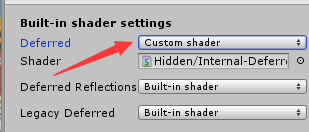
\includegraphics[width=.9\linewidth]{./pic/builtinshader.png}
\end{center}
\end{enumerate}

\subsubsection{Lagacy Deferred Lighting Rendering Path(延迟光照)}
\label{sec:orge9f7adc}
\begin{itemize}
\item 官方文档:\url{http://docs.unity3d.com/Manual/RenderTech-DeferredLighting.html}
\item 技术文章:\url{http://www.realtimerendering.com/blog/deferred-lighting-approaches/}
\begin{itemize}
\item 注:从5.0开始,DL渲染已经不被Unity3D推荐,Unity3D更推荐大家新项目使用DS管线方式。因为DL方式不好实现基于PBR着色的Standard材质,以及场景反射。
\item 注:如果摄像机设置为了正交投影。会强制退回前向渲染
\item 注:DL也不会降低实时阴影的开销
\end{itemize}
\item 和DS渲染管线一样,DL的出现同样是为了解决光照计算的复杂度问题。然后不同的是,DL仅仅把光照计算拿出去了。简单说来,DL管线工作流程如下。
\begin{itemize}
\item 步骤一、渲染场景中的对象,输出光照计算需要的RT(深度、法线、高光信息)
\item 步骤二、使用上面的RT进行光照计算
\item 步骤三、再次渲染场景中的对象,并与计算机来的光照信息结合。
\end{itemize}
\item 不难看出,DL相比DS而言,不需要大量的G-Buffer支持。甚至不需要MRT的支持。但是对深度图的要求是必须的。如果遇上无法访问深度BUFFER的情况。那就需要做一次Pre-Depth Pass渲染。
\item 比起DS而言,DL由于不需要MRT的支持。在硬件特性需求和位宽上,少了许多开销。
\begin{itemize}
\item 1、SM3.0
\item 2、PC:GeForce FX、Radeon X1300、Intel 965 / GMA X3100
\item 3、Mobile:所有支持OpenGL ES 3.0的设备,部分支持OpenGL ES 2.0的设备。
\end{itemize}
\end{itemize}

\subsubsection{Vertex Lit Rendering Path(顶点光照)}
\label{sec:org0eba7a1}
\begin{itemize}
\item 官方文档:\url{http://docs.unity3d.com/Manual/RenderTech-VertexLit.html}
\begin{itemize}
\item 注:这不是一个通用的技术名词,只有Unity3D中有。
\item 注:主机平台这个不顶用。
\item 注:不支持实时阴影和高精度高光计算。
\end{itemize}
\item Vertex Lit Rendering就是指,所有的光照计算都通过顶点进行。而在Unity3D中,它的主要目的是为了支持那些没有可编程管线的设备。VL也提供了几种方法,用于支持不同的材质类型。
\begin{itemize}
\item 1、Vertex 使用Blinn-Phong进行光照处理,针对没有lightmap的对象使用。
\item 2、VertexLMRGBM 针对lightmap贴图使用RGBM加密(PC和主机平台)的对象, 没有额外的光照计算。
\item 3、VertexLMM 针对lightmap贴图使用double-LDR加密(移动平台)的对象,没有额外的光照计算。
\end{itemize}
\end{itemize}
\subsubsection{Unity3D对几种渲染管线的统一处理}
\label{sec:orga626f98}
\begin{itemize}
\item 在上面我描述中,我们发现,不管哪一种管线。都会涉及到几个部分。 
\begin{itemize}
\item 1、光照计算
\item 2、透明渲染
\item 3、阴影计算
\item 4、图像输出。
\end{itemize}
\item 那Unity3D又是如何对这些进行统一流程控制的呢。我们看下面的图就明白了。

\begin{figure}[htbp]
\centering
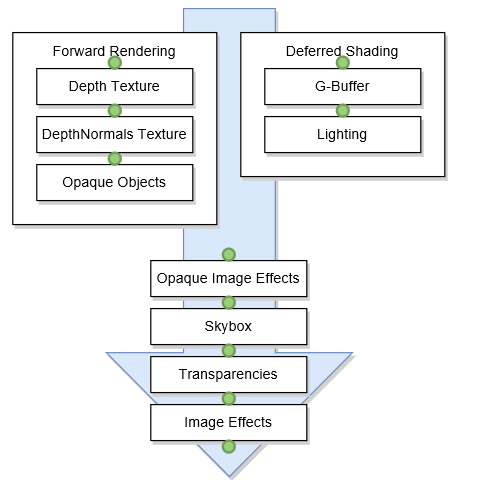
\includegraphics[width=.9\linewidth]{./pic/rendering.png}
\caption{Unity3D渲染管线图}
\end{figure}
\item 从图中我们可以看到。Unity3D的传统渲染管线和延迟渲染管线,在非透明物体渲染和光照阶段是分离的。当处理完以后,紧接着处理非透明图像效果->天空盒->透明物体渲染->后期效果。
\end{itemize}
\subsubsection{结束语}
\label{sec:orgbda4016}
\begin{itemize}
\item 总的来说,Unity3D的渲染管线还算稳定和易用,其的渲染管线包含了常见的三种方案。最主要目的还是在想着光照计算和效果显示的处理。同时保持对上层透明。其Graphics Commander Buffer提供了扩展管线的能力。而Graphics设置面板里,也提供了自定义延迟管线Shader的功能。然而也有诸多的美中不足,比如,正交摄像机模式下,不能使用延迟渲染技术。 延迟光照下无法实现PBR和实时环境反射抽取等等。
\end{itemize}

\subsection{Unity5 Lighting面板说明书}
\label{sec:org6aa22d1}
\begin{itemize}
\item \url{https://blog.csdn.net/u010026134/article/details/53673015}
\end{itemize}
\subsubsection{Object面板}
\label{sec:org20a2a34}
\begin{itemize}
\item Lightmap Static: 当前所选物体是否有勾上Lightmap Static。如果该物体没有勾上Lightmap Static,仍可用光线探针(Light Probe)来照亮。
\item Scale In Lightmap: 该值影响当前物体对应lightmap上的像素数。默认值 1 代表像素数只取决于该物体表面区域(也就是说,各区域像素数相同)。该值越大(大于1),像素数越多;该值越小(小于1),像素数越少(lightmap分辨率)。调整该值,有利于优化lightmap,使重点细节区得到更精确的照射。举个例子,场景是带平坦黑色墙壁的某独立建筑,此时用小一点儿的lightmap scale(小于1)会更合适;若场景是一堆五颜六色的摩托车,用大点儿的值更合适。
\item Important GI: 勾上,代表告诉Unity当前选择物体的光反射/放射会以显眼的方式影响其它物体,不让Unity优化该光源效果。
\item Advanced Parameters: 当前选择物体的高级lightmap设置(可选择或创建)。
\item Preserve UVs: 是否保护UV坐标(又可以叫"是否接受UV优化")。为了提高性能,Unity会重新计算实时光照贴图的UV坐标。而在重新计算时,有时会对原UV坐标连续性判断出错。举个例子,把锐角错误判断成曲面。若勾上"保护UV坐标",则保留原有UV的效果;若不勾,则Unity会基于已烘培UV,计算实时光照贴图UV,加入临近Charts,尽可能使lightmap紧凑。计算过程和下方max distance, max angle有关。实时Charts被半像素的边界包围,保证渲染时不会发生遗漏。
\item Auto UV Max Distance: 如果Charts之间的worldspace距离比该值小,则简化Charts。
\item Auto UV Max Angle: 如果Charts之间的角度比该值小,则简化Charts。
\item Ignore Normals: 在实时全局光照检测Charts时,请勿比较法线(就是说这里要打勾)。手动编辑UV坐标时,可勾上该选项,以避免出现Chart分离问题。
\item Min Chart Size: 这里涉及到Unity全新光照系统Enlighten的缝合特性,该特性使Chart平滑缝合(连接)在一起(比如说球体和圆柱体)。该特性需要每个Chart的每条边的方向数据,而方向数据是以块(block)单位存储的,则每个可缝合Chart最少需要2*2块。如果不需要精确缝合效果(比如说台阶模型),可选择2(Minimum)。

\begin{center}
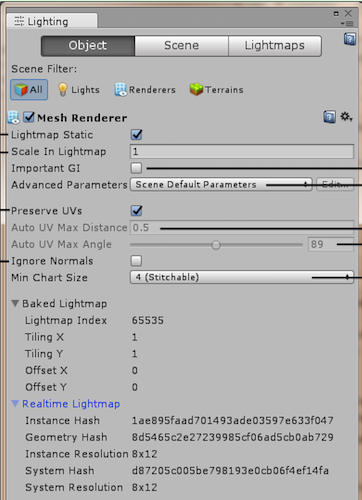
\includegraphics[width=.9\linewidth]{./pic/lighting_obj.png}
\end{center}

\begin{center}
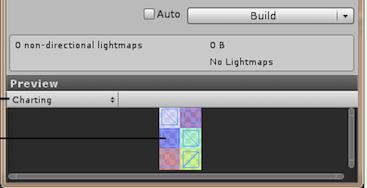
\includegraphics[width=.9\linewidth]{./pic/lighting_obj2.png}
\end{center}
\item Charting: 这个彩图就是Chart,里面的蓝色线框就是当前选择模型的UV(也可在Scene视图的UV Charts模式下浏览)。

\begin{center}
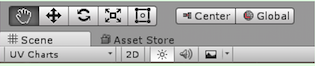
\includegraphics[width=.9\linewidth]{./pic/uvchart.png}
\end{center}
\end{itemize}
\subsubsection{Scene面板}
\label{sec:org0139a62}
\begin{itemize}
\item Environment Lighting: 环境光照
\begin{itemize}
\item Sun: 当使用天空盒时,可在此设置代表太阳的平行光(或者其它够大够远的照亮场景的光源)。如果设置为None,则假定场景中最亮的平行光代表太阳。
\item Ambient Source: 环境光源
\item Ambient Intensity: 环境光亮度
\item Ambient GI: 指定环境光的全局光照模式
\item Reflection Source: 反向源,使用天空盒(天空盒也是Cubemap)或其它自定义Cubemap。如果不需要反射,请选自定义Cubemap但不赋值,这样就不会生成反射探针(Reflection Probe)。
\item Resolution: Cubemap分辨率
\item Compression: 是否需要压缩反射探针(Reflection Probe)
\item Reflection Intensity: 在反射物上反射源(天空盒或自定义Cubemap)的可见程度
\item Reflection Bounces: 反弹反射。在场景中用反射探针(Reflection Probe)捕捉该反射。该值决定了反射探针所检测物体之间的来回反射反弹次数。如果该值为1,则只有初始反射(即来自上述Reflection Source的Skybox/自定义Cubemap的反射)。
\end{itemize}

\begin{center}
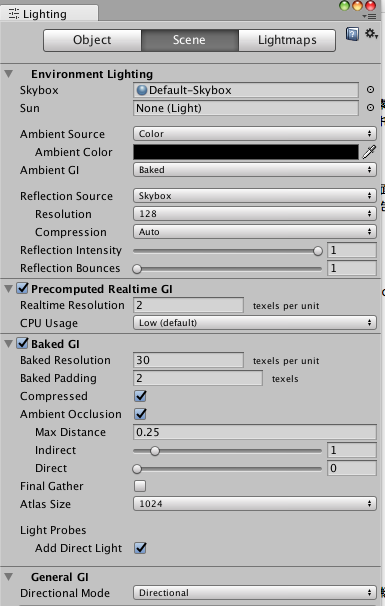
\includegraphics[width=.9\linewidth]{./pic/lighting_scene1.png}
\end{center}
\item Precomputed Realtime GI: 预处理实时全局光照
\begin{itemize}
\item Realtime Resolution: 实时lightmap分辨率,每世界坐标单位多少纹素,通常每单位一纹素就已经有不错的效果,如果是地形或大型物体,请适量调低该值。
\item CPU Usage: 运行时最终光照计算的CPU占用
\end{itemize}
\item Baked GI: 烘培式全局光照
\begin{itemize}
\item Baked Resolution: 烘培式lightmap分辨率,每世界坐标多少纹素
\item Baked Padding: 在lightmap上图形之间相距有多少纹素
\item Compressed: 是否压缩烘培式lightmap(压缩后的lightmap可能会产生伪影)
\item Indirect Resolution: (只在Precomputed Realtime GI没有勾时才出现)计算间接照明分辨率。该数值等同Precomputed Realtime GI中的Realtime Resolution。
\item Ambient Occlusion: 环境光遮蔽区表面的相对亮度值。该值越大,遮蔽区和无遮蔽区对比越鲜明
\item Final Gather: "最终收集"。当勾上时,在同分辨率已烘培lightmap中计算最终光反弹量。能提高lightmap可视性,但需要耗费额外的烘培时间。
\item Atlas Size: 整张lightmap贴图的纹素大小
\item Light Probes: 光线探针
\item Add Direct Light: 在光线探针中加入平行光。如果整个场景都用烘培式照明,但又需要有动态物体照明,请勾上该选项。如果场景实时照明,则光线探针只能放间接光
\end{itemize}
\item General GI: 一般全局光照
\begin{itemize}
\item Directional Mode: 通过设置lightmap的directional模式,可以存储物体表面每一点的主导入射光信息。在directional模式下,会生成第二张lightmap来存储主导入射光信息。Directional Specular模式下,主要是配合漫反射法线贴图,甚至是高光反射法线贴图工作。Directional模式需要两倍空间存储额外的lightmap数据,而Directional Specular需要四倍存储空间和两倍纹理内存
\item Indirect Intensity: 间接照明亮度值
\item Bounce Boost: 反弹(物体表面之间光反弹)增量
\item Default Parameters: 当前场景的默认Lightmap设置(可选择或创建)
\end{itemize}

\begin{center}
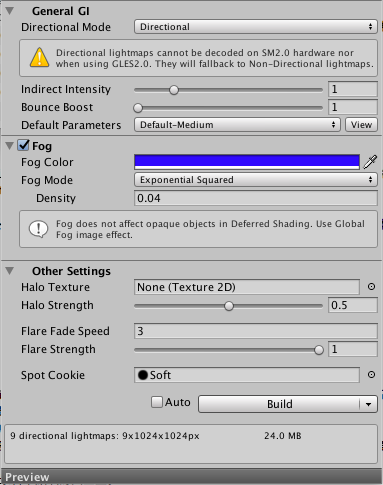
\includegraphics[width=.9\linewidth]{./pic/lighting_scene2.png}
\end{center}
\item Fog: 雾效
\begin{itemize}
\item Fog Color: 雾的颜色(如果渲染路径选择延迟渲染,则雾效不起作用)
\item Fog Mode: 雾效累积模式(线性累积、指数累积、指数平方累积)
\item Density: 雾效密度
\end{itemize}
\item Other Settings: 其它设置
\begin{itemize}
\item Halo Texture: 光晕贴图
\item Halo Strength: 光晕能见度
\item Flare Fade Speed: 镜头光晕淡出时间
\item Flare Strength: 镜头光晕能见度
\item Spot Cookie: 聚光灯(Spot Light)所用剪影(Cookie)
\end{itemize}
\end{itemize}

\subsubsection{Stats面板}
\label{sec:orgaa0281d}
\begin{itemize}
\item \url{http://www.voidcn.com/article/p-kegvverb-ha.html}
\item Unity5的 Statistics上的统计信息和Unity4 有一些区别,
\item Statistics窗口,全称叫做 Rendering Statistics Window,即渲染统计窗口(或渲染数据统计窗口),
\item 窗口中罗列出关于渲染、声音、网络状况等多种统计信息 ,下面详细的解释一下这些项的意义。
\end{itemize}

\begin{center}
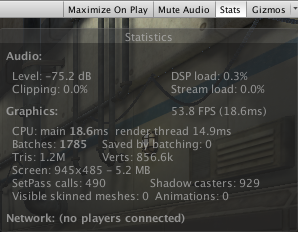
\includegraphics[width=.9\linewidth]{./pic/stats.png}
\end{center}
\begin{itemize}
\item FPS
\item FPS(Time per frame andFPS):frames per seconds表示引擎处理和渲染一个游戏帧所花费的时间,该数字主要受到场景中渲染物体数量和 GPU性能的影响,FPS数值越高,游戏场景的动画显示会更加平滑和流畅。一般来说,超过30FPS的画面人眼不会感觉到卡,由于视觉残留的特性,光在视网膜上停止总用后人眼还会保持1/24秒左右的时间,因此游戏画面每秒帧数至少要保证在30以上。
\item 另外,Unity中的FPS数值仅包括此游戏Scene里更新和渲染的帧,编辑器中绘制的Scene和其它监视窗口的进程不包括在内。
\item CPU
\begin{itemize}
\item CPU:获取到当前占用CPU进行计算的时间绝对值,或时间点,如果Unity主进程处于挂断或休眠状态时,CPU time将会保持不变。
\end{itemize}
\item Render thread
\begin{itemize}
\item Render thread:GPU渲染线程处理图像所花费的时间,具体数值由GPU性能来决定
\end{itemize}
\item Batches
\begin{itemize}
\item Batches:即Batched Draw Calls,是Unity内置的Draw Call Batching技术。
\item 首先解释下什么叫做“Draw call”,CPU每次通知GPU发出一个glDrawElements(OpenGl中的图元渲染函数)或者 DrawIndexedPrimitive(DirectX中的顶点绘制方法)的过程称为一次Draw call,一般来说,引擎每对一个物体进行一次DrawCall,就会产生一个Batch,这个Batch里包含着该物体所有的网格和顶点数据,当渲染另一个相同的物体时,引擎会直接调用Batch里的信息,将相关顶点数据直接送到GPU,从而让渲染过程更加高效,即Batching技术是将所有材质相近的物体进行合并渲染。
\item 对于含有多个不同Shader和Material的物体,渲染的过程比较耗时,因为会产生多个Batches。每次对物体的材质或者贴图进行修改,都会影响Batches里数据集的构成。因此,如果场景中有大量材质不同的物体,会很明显的影响到GPU的渲染效率。这里说几点关于Batches优化相关的方案
\item 虽然Unity引擎自带Draw Call Batching技术,我们也可以通过手动的方式合并材质接近的物体;
\item 尽量不要修改Batches里物体的Scale,因为这样会生成新的Batch。
\item 为了提升GPU的渲染效率,应当尽可能的在一个物体上使用较少的材质,减少Batches过多的开销;
\item 对于场景中不会运动的物体,考虑设置Static属性,Static声明的物体会自动进行内部批处理优化。
\end{itemize}
\item Verts和Tris  
\begin{itemize}
\item Verts:摄像机视野(field of view)内渲染的顶点总数。
\item Tris:   摄像机视野(field of view)内渲染的的三角面总数量。                                                                                                                             - 关于Tris和Verts,突然想到一些问题,这里需要多嘴说几句:
\item Camera的渲染性能受到Draw calls的影响。之前说过,对一个物体进行渲染,会生成相应的Draw call,处理一个Draw Call的时间是由它上边的Tris和Verts数目决定。尽可能得合并物体,会很大程度的提高性能。举个很简单例子,比如场景一种有1000个不同的物体,每个物体都有10个Tris;场景二中有10个不同的物体,每个物体有1000个Tris。在渲染处理中,场景一中会产生1000个Draw Calls,它的渲染时间明显比场景二慢。
\item Unity stats 视图中的 Tris 和 Verts 并不仅仅是视锥中的梯形内的 Tris 和 Verts,而是Camera中 field of view所有取值下的tris和verts,换句话说,哪怕你在当前game视图中看不到这个 cube,如果当你把 field of view调大到 179 过程中都看不到这个cube,stats面板才不会统计,GPU才不会渲染,否则都会渲染,而且unity不会把模型拆分,这个模型哪怕只有1个顶点需要渲染,unity也会把整个模型都渲出来。(参考自Mess的《Unity Camera组件部分参数详解》)
\item 之前有童鞋问过我,新建一个空的场景,里边没有添加任何物体,为什么Status面板上显示有1.7k Tris以及5.0kVerts。这是因为空的场景自带默认的天空盒。
\item 点击Windows---Lighting打开Lighting下的Scene面板,把Skybox里的材质设为空
\item 删掉它,你就会发现Tris 和 Verts 都变为0了(以Unity 5.5.0为例)
\end{itemize}
\item Screen
\begin{itemize}
\item Screen:获当前Game屏幕的分辨率大小,后边的2.1MB表示总的内存使用数值。
\end{itemize}
\item SetPass calls
\begin{itemize}
\item SetPass calls:在Unity 4.x和3.x原来的Stats面板的第一项是“Draw calls”,然而到了Unity5.X版本,Stats上没有了“Draw calls”,却多出来一项”SetPass calls“。
\item 比如说场景中有100个gameobject,它们拥有完全一样的Material,那么这100个物体很可能会被Unity里的Batching机制结合成一个Batch。所以用“Batches”来描述Unity的渲染性能是不太合适的,它只能反映出场景中需要批处理物体的数量。那么可否用“Draw calls”来描述呢?答案同样是不适合。每一个“Draw calls”是CPU发送个GPU的一个渲染请求,请求中包括渲染对象所有的顶点参数、三角面、索引值、图元个数等,这个请求并不会占用过多的消耗,真正消耗渲染资源的是在GPU得到请求指令后,把指令发送给对应物体的Shader,让Shader读取指令并通知相应的渲染通道(Pass)进行渲染操作。
\item 假设场景中有1个gameobject,希望能显示很酷炫的效果,它的Material上带有许多特定的Shader。为了实现相应的效果,Shader里或许会包含很多的Pass,每当GPU即将去运行一个Pass之前,就会产生一个“SetPass call”,因此在描述渲染性能开销上,“SetPass calls”更加有说服力。
\end{itemize}
\item Shadow casters
\begin{itemize}
\item Shadow casters:表示场景中有多少个可以投射阴影的物体,一般这些物体都作为场景中的光源。
\end{itemize}
\item visible skinned  meshed
\begin{itemize}
\item visible skinned  meshed:渲染皮肤网格的数量。
\end{itemize}
\item Animations
\begin{itemize}
\item Animations:正在播放动画的数量。
\end{itemize}
\item 其它
\begin{itemize}
\item 目前渲染统计窗口的参数就只有这些,如果你想了解更多的渲染信息,可以打开Unity的Profiler窗口(右键--AddTab---Profiler),这儿你可以获取到更多的渲染数据,比如“Draw Calls”、"VBO Totals"、"VB Uploads"等等,还能实时观察CPU、内存和音频的使用情况。
\end{itemize}
\end{itemize}

\subsection{Unity3D Mesh学习笔记 -- 创建MeshBuilder}
\label{sec:orgce630b1}
\begin{itemize}
\item \url{http://www.voidcn.com/article/p-ubvbgmhq-pe.html}
\begin{minted}[linenos=true]{csharp}
using UnityEngine;
using System.Collections;
using System.Collections.Generic;

// 实现了MeshBuilder的类,会使得我们生成mesh的时候犯的错误更少一些
public class MeshBuilder   {

	private List<Vector3> m_Vertices = new List<Vector3>();
	public List<Vector3> Vertices {get{return m_Vertices; }}

    private List<Vector3> m_Normals = new List<Vector3>();
	public List<Vector3> Normals {get{return m_Normals; }}

    private List<Vector2> m_UVs = new List<Vector2>();
	public List<Vector2> UVs {get{return m_UVs; }}

    private List<int> m_indexs = new List<int>();
	
	public void AddTriangle(int index0, int index1, int index2) {
        m_indexs.Add (index0);
        m_indexs.Add (index1);
        m_indexs.Add (index2);
    }

    public Mesh CreateMesh() {
        Mesh mesh = new Mesh ();
        mesh.vertices = m_Vertices.ToArray ();
        mesh.triangles = m_indexs.ToArray ();
        if (m_Normals.Count == m_Vertices.Count)
            mesh.normals = m_Normals.ToArray ();
        if (m_UVs.Count == m_Vertices.Count)
            mesh.uv = m_UVs.ToArray ();
        mesh.RecalculateBounds ();
        return mesh;
    }
}

public class MeshBuilderTest : MonoBehaviour {

	private float m_Length = 1f;
	private float m_Width = 1f;
	
	public void Start() {
        TestMeshBuilder ();
    }
	
	public void TestMeshBuilder() {
        MeshBuilder meshBuilder = new MeshBuilder();
		
        //Set up the vertices and triangles:
        meshBuilder.Vertices.Add(new Vector3(0.0f, 0.0f, 0.0f));
        meshBuilder.UVs.Add(new Vector2(0.0f, 0.0f));
        meshBuilder.Normals.Add(Vector3.up);
		
        meshBuilder.Vertices.Add(new Vector3(0.0f, 0.0f, m_Length));
        meshBuilder.UVs.Add(new Vector2(0.0f, 1.0f));
        meshBuilder.Normals.Add(Vector3.up);
		
        meshBuilder.Vertices.Add(new Vector3(m_Width, 0.0f, m_Length));
        meshBuilder.UVs.Add(new Vector2(1.0f, 1.0f));
        meshBuilder.Normals.Add(Vector3.up);
		
        meshBuilder.Vertices.Add(new Vector3(m_Width, 0.0f, 0.0f));
        meshBuilder.UVs.Add(new Vector2(1.0f, 0.0f));
        meshBuilder.Normals.Add(Vector3.up);
		
        meshBuilder.AddTriangle(0, 1, 2);
        meshBuilder.AddTriangle(0, 2, 3);
		
        MeshFilter filter = this.gameObject.AddComponent<MeshFilter> ();
        if (filter != null) {
            filter.sharedMesh = meshBuilder.CreateMesh();
        }
		
        MeshRenderer meshRender = this.gameObject.AddComponent<MeshRenderer> ();
        Shader shader = Shader.Find ("Diffuse");
        meshRender.sharedMaterial = new Material (shader);
    }
}
\end{minted}
\end{itemize}

\subsection{深入了解光照贴图}
\label{sec:orgbbf8cad}
\begin{itemize}
\item \url{https://my.oschina.net/u/2874878/blog/736785}
\end{itemize}

\section{Unity ShaderLab学习总结}
\label{sec:org37ec4d6}
\subsection{Shader基础}
\label{sec:org3dd8fbd}
\subsubsection{SubShader的Tag}
\label{sec:org5d44b7a}
\begin{minted}[linenos=true]{python}
Shader "ShaderLab Tutorials/TestShader" {
    SubShader
    {
        Tags { "Queue"="Geometry+10" "RenderType"="Opaque" }
        //...
    }
}
\end{minted}

SubShader内部可以有标签(Tags)的定义。Tag指定了这个SubShader的渲染顺序(时机),以及其他的一些设置。

\begin{enumerate}
\item "RenderType"标签。Unity可以运行时替换符合特定RenderType的所有Shader。Camera.RenderWithShader或Camera.SetReplacementShader配合使用。Unity内置的RenderType包括:
\label{sec:orgd1e1ca4}
\begin{itemize}
\item "Opaque":绝大部分不透明的物体都使用这个;
\item "Transparent":绝大部分透明的物体、包括粒子特效都使用这个;
\item "Background":天空盒都使用这个;
\item "Overlay":GUI、镜头光晕都使用这个;
\end{itemize}

用户也可以定义任意自己的RenderType这个标签所取的值。

应注意,Camera.RenderWithShader或Camera.SetReplacementShader不要求标签只能是RenderType,RenderType只是Unity内部用于Replace的一个标签而已,你也可以自定义自己全新的标签用于Replace。

比如,你为自己的ShaderA.SubShaderA1(会被Unity选取到的SubShader,常为Shader文件中的第一个SubShader)增加Tag为"Distort"\texttt{"On",然后将"Distort"作为参数replacementTag传给函数。此时,作为replacementShader实参的ShaderB.SubShaderB1中若有也有一模一样的"Distort"}"On",则此SubShaderB1将代替SubShaderA1用于本次渲染。

具体可参考Rendering with Replaced Shaders \url{https://docs.unity3d.com/Manual/SL-ShaderReplacement.html}

\item "Queue"标签。定义渲染顺序。预制的值为
\label{sec:orgcf82ea1}
\begin{itemize}
\item "Background"。值为1000。比如用于天空盒。
\item "Geometry"。值为2000。大部分物体在这个队列。不透明的物体也在这里。这个队列内部的物体的渲染顺序会有进一步的优化(应该是从近到远,early-z test可以剔除不需经过FS处理的片元)。其他队列的物体都是按空间位置的从远到近进行渲染。
\item "AlphaTest"。值为2450。已进行AlphaTest的物体在这个队列。
\item "Transparent"。值为3000。透明物体。
\item "Overlay"。值为4000。比如镜头光晕。
\item 用户可以定义任意值,比如"Queue"="Geometry+10"
\item "ForceNoShadowCasting",值为"true"时,表示不接受阴影。
\item "IgnoreProjector",值为"true"时,表示不接受Projector组件的投影。
\end{itemize}

另,关于渲染队列和Batch的非官方经验总结是,一帧的渲染队列的生成,依次决定于每个渲染物体的:

\begin{itemize}
\item Shader的RenderType tag,
\item Renderer.SortingLayerID,
\item Renderer.SortingOrder,
\item Material.renderQueue(默认值为Shader里的"Queue"),
\item Transform.z(ViewSpace)(默认为按z值从前到后,但当Queue是“Transparent”的时候,按z值从后到前)。
\end{itemize}

这个渲染队列决定了之后(可能有dirty flag的机制?)渲染器再依次遍历这个渲染队列,“同一种”材质的渲染物体合到一个Batch里。
\end{enumerate}

\subsubsection{Pass}
\label{sec:org0e4896a}
\begin{minted}[linenos=true]{python}
Shader "ShaderLab Tutorials/TestShader" {
    SubShader {
        Pass
        {
            //...
        }
    }
}
\end{minted}
一个SubShader(渲染方案)是由一个个Pass块来执行的。每个Pass都会消耗对应的一个DrawCall。在满足渲染效果的情况下尽可能地减少Pass的数量。

\begin{enumerate}
\item Pass的Tag
\label{sec:org05a496e}
\begin{minted}[linenos=true]{python}
Shader "ShaderLab Tutorials/TestShader" {
    SubShader {
        Pass
        {
            Tags{ "LightMode"="ForwardBase" }
            //...
        }
    }
}
\end{minted}

和SubShader有自己专属的Tag类似,Pass也有Pass专属的Tag。

其中最重要Tag是 "LightMode",指定Pass和Unity的哪一种渲染路径(“Rendering Path”)搭配使用。除最重要的ForwardBase、ForwardAdd外,这里需额外提醒的Tag取值可包括:

\begin{itemize}
\item Always,永远都渲染,但不处理光照
\item ShadowCaster,用于渲染产生阴影的物体
\item ShadowCollector,用于收集物体阴影到屏幕坐标Buff里。
\item 其他渲染路径相关的Tag详见下面章节“Unity渲染路径种类”。
\item 具体所有Tag取值,可参考ShaderLab syntax: Pass Tags。
\end{itemize}

\item FallBack
\label{sec:org9b4f056}
\begin{minted}[linenos=true]{python}
Shader "ShaderLab Tutorials/TestShader"{
    SubShader { Pass {} }

    FallBack "Diffuse" // "Diffuse"即Unity预制的固有Shader
    // FallBack Off //将关闭FallBack
}
\end{minted}

当本Shader的所有SubShader都不支持当前显卡,就会使用FallBack语句指定的另一个Shader。FallBack最好指定Unity自己预制的Shader实现,因其一般能够在当前所有显卡运行。

\item Properties
\label{sec:org34c3b8d}

\begin{minted}[linenos=true]{python}
Shader "ShaderLab Tutorials/TestShader"
{
    Properties {
    _Range ("My Range", Range (0.02,0.15)) = 0.07 // sliders
    _Color ("My Color", Color) = (.34, .85, .92, 1) // color
    _2D ("My Texture 2D", 2D) = "" {} // textures
    _Rect("My Rectangle", Rect) = "name" { }
    _Cube ("My Cubemap", Cube) = "name" { }
    _Float ("My Float", Float) = 1
    _Vector ("My Vector", Vector) = (1,2,3,4)

    // Display as a toggle.
    [Toggle] _Invert ("Invert color?", Float) = 0
    // Blend mode values
    [Enum(UnityEngine.Rendering.BlendMode)] _Blend ("Blend mode", Float) = 1
    //setup corresponding shader keywords.
    [KeywordEnum(Off, On)] _UseSpecular ("Use Specular",  Float) = 0
    }

    // Shader
    SubShader{
        Pass{
          //...
          uniform float4 _Color;
          //...
          float4 frag() : COLOR{ return fixed4(_Color); }
          //...
             #pragma multi_compile __ _USESPECULAR_ON
          }
    }

    //fixed pipeline
    SubShader    {
        Pass{
            Color[_Color]
        }
    }
}
\end{minted}

\begin{itemize}
\item Shader在Unity编辑器暴露给美术的参数,通过Properties来实现。
\item 所有可能的参数如上所示。主要也就Float、Vector和Texture这3类。
\item 除了通过编辑器编辑Properties,脚本也可以通过Material的接口(比如SetFloat、SetTexture编辑)
\item 之后在Shader程序通过[name](固定管线)或直接name(可编程Shader)访问这些属性。
\item 在每一个Property前面也能类似C\#那样添加Attribute,以达到额外UI面板功能。详见MaterialPropertyDrawer.html。
\end{itemize}
\end{enumerate}
\subsubsection{Shader中的数据类型}
\label{sec:orgd4af8b9}

有3种基本数值类型:float、half和fixed。

这3种基本数值类型可以再组成vector和matrix,比如half3是由3个half组成、float4x4是由16个float组成。

\begin{itemize}
\item float:32位高精度浮点数。
\item half:16位中精度浮点数。范围是[-6万, +6万],能精确到十进制的小数点后3.3位。
\item fixed:11位低精度浮点数。范围是[-2, 2],精度是1/256。
\end{itemize}

数据类型影响性能

\begin{itemize}
\item 精度够用就好。
\item 颜色和单位向量,使用fixed
\item 其他情况,尽量使用half(即范围在[-6万, +6万]内、精确到小数点后3.3位);否则才使用float。
\end{itemize}
\subsubsection{ShaderLab中的Matrix}
\label{sec:orgb82cd44}

当提到“Row-Major”、“Column-Major”,根据不同的场合,它们可能指不同的意思:

\begin{itemize}
\item 数学上的,主要是指矢量V是Row Vector、还是Column Vector。引用自[Game Engine Architecture 2nd Edition, 183]。留意到V和M的乘法,当是Row Vector的时候,数学上写作VM,Matrix在右边,Matrix的最下面一行表示Translate;当是Column Vector的时候,数学上写作MtVt,Matrix在左边并且需要转置,Matrix最右面一列表示Translate。
\item 访问接口上的:Row-Major即MyMatrix[Row][Column]、Column-Major即MyMatrix[Column][Row]。HLSL/CG的访问接口都是Row-Major,比如MyMatrix[3]返回的是第3行;GLSL的访问接口是Column-Major,比如MyMatrix[3]返回的是第3列。
\item 寄存器存储上的:每个元素是按行存储在寄存器中、还是按列存储在寄存器中。需要关注它的一般情况举例是,float2x3的MyMatrix,到底是占用2个寄存器(Row-Major)、还是3个寄存器(Column-Major)。在HLSL里,可以通过\#pragmapack\textsubscript{matrix设定row}\textsubscript{major或者column}\textsubscript{major}。
\end{itemize}

上述情况,互不相干。

然后,ShaderLab中,数学上是Column Vector、访问接口上是Row-Major、存储上是(尚未查明)。

\subsubsection{ShaderLab中各个Space的坐标系}
\label{sec:org5fdd735}

一般情况下,从Vertex Buff输入顶点到Vertex Shader,

\begin{itemize}
\item 该顶点为左手坐标系Model Space中的顶点vInModel,
\item 其用w=1的Homogenous Cooridniates(故等效于Cartesian Coordinates)表达vInModel = float4(xm, ym, zm, 1);
\item vInWrold = mul(\textsubscript{Object2World} , vInModel)后,得出左手坐标系World Space中的vInWorld,其为w=1的Homogenous Cooridniates(故等效于Cartesian Coordinates)vInWorld = float4(xw, yw, zw, 1);
\item vInView = mul(UNITY\textsubscript{MATRIX}\textsubscript{V} , vInWrold)后,得出右手坐标系View Space中的vInView,其为w=1的Homogenous Cooridniates(故等效于Cartesian Coordinates)vInWorld = float4(xv, yv, zv, 1);
\item vInClip = mul(UNITY\textsubscript{MATRIX}\textsubscript{P} , vInView)后,得出左手坐标系Clip Space中的vInClip,其为w往往不等于1的Homogenous Cooridniates(故往往不等效于Cartesian Coordinates)vInClip = float4(xc, yc, zc, wc);
\end{itemize}

设r、l、t、b、n、f的长度绝对值如下图:

\begin{center}
\includegraphics[width=.9\linewidth]{./pic/tl.png}
\end{center}

注意View Space中摄像机前方的z值为负数、-z为正数。则GL/DX/Metal的Clip Space坐标为:
\begin{itemize}
\item GL:
\begin{itemize}
\item xc=(2nx+rz+lz)/(r-l);
\item yc=(2ny+tz+bz)/(t-b);
\item zc=(-fz-nz-2nf)/(f-n);
\item wc=-z;
\end{itemize}
\item DX/Metal:
\begin{itemize}
\item xc=(2nx+rz+lz)/(r-l);
\item yc=(2ny+tz+bz)/(t-b);
\item zc=(-fz-nf)/(f-n);
\item wc=-z;
\end{itemize}
\item vInNDC = vInClip / vInClip.w后,得出左手坐标系Normalized Device Coordinates中的vInNDC,其为w=1的Homogenous Cooridniates(故等效于Cartesian Coordinates)vInNDC = float4(xn, yn, zn, 1)。xn和yn的取值范围为[-1,1]。
\begin{itemize}
\item GL: zn=zc/wc=(fz+nz+2nf)/((f-n)z);
\item DX/Metal: zn=zc/wc=(fz+nf)/((f-n)z);
\item 在Unity中,zn的取值范围可以这样决定:
\begin{itemize}
\item 如果UNITY\textsubscript{REVERSED}\textsubscript{Z已定义},zn的取值范围是[UNITY\textsubscript{NEAR}\textsubscript{CLIP}\textsubscript{VALUE}, 0],即[1,0]
\item 如果UNITY\textsubscript{REVERSED}\textsubscript{Z未定义},zn的取值范围是[UNITY\textsubscript{NEAR}\textsubscript{CLIP}\textsubscript{VALUE}, 1]
\begin{itemize}
\item 如果SHADER\textsubscript{API}\textsubscript{D3D9}/SHADER\textsubscript{API}\textsubscript{D3D11}\textsubscript{9X定义了},即[0,1]
\item 否则,即OpenGL情况,即[-1,1]
\end{itemize}
\end{itemize}

\begin{minted}[linenos=true]{python}
v2f vert (appdata v)
{
    v2f o;
    o.vertex = mul(UNITY_MATRIX_MVP, v.vertex);
    // 1 、2、3是等价的,和4是不等价的
    // 因为是M在左、V在右,所以是Column Vector
    // 因为是HLSL/CG语言,所以是访问方式是Row-Major
    o.rootInView = mul(UNITY_MATRIX_MV, float4(0, 0, 0, 1)); // 1
    o.rootInView = float4(UNITY_MATRIX_MV[0].w, UNITY_MATRIX_MV[1].w, UNITY_MATRIX_MV[2].w, 1); // 2                
    o.rootInView = UNITY_MATRIX_MV._m03_m13_m23_m33;  // 3
    //o.rootInView = UNITY_MATRIX_MV[3]; // 4

    return o;
}

fixed4 frag (v2f i) : SV_Target
{
    // 因为是ViewSpace是右手坐标系,所以当root在view前面的时候,z是负数,所以需要-z才能正确显示颜色
    fixed4 col = fixed4(i.rootInView.x, i.rootInView.y, -i.rootInView.z, 1);
    return col;
}

struct appdata
{
    float4 vertex : POSITION;
};
struct v2f
{
    float4 rootInView : TEXCOORD0;
    float4 vertex : SV_POSITION;
};
\end{minted}
\end{itemize}
\end{itemize}

\subsection{Shader形态}
\label{sec:org7a841c4}

\subsubsection{Shader形态之1:固定管线}
\label{sec:org0f24bf9}
固定管线是为了兼容老式显卡。都是顶点光照。之后固定管线可能是被Unity抛弃的功能,所以最好不学它、当它不存在。特征是里面出现了形如下面Material块、没有CGPROGRAM和ENDCG块。
\begin{minted}[linenos=true]{python}
Shader "ShaderLab Tutorials/TestShader"
{
    Properties {
    _Color ("My Color", Color) = (.34, .85, .92, 1) // color
    }

    // Fixed Pipeline
    SubShader
    {
        Pass
        {
            Material{
            Diffuse [_Color]
            Ambient [_Color]
            }

            Lighting On
        }
    }
}
\end{minted}
\subsubsection{Shader形态之2:可编程Shader}
\label{sec:org817b793}
\begin{minted}[linenos=true]{python}
Shader "ShaderLab Tutorials/TestShader"
{
    Properties {}

    SubShader
    {
        Pass
        {
          // ... the usual pass state setup ...

          CGPROGRAM
          // compilation directives for this snippet, e.g.:
          #pragma vertex vert
          #pragma fragment frag

          // the Cg/HLSL code itself
          float4 vert(float4 v:POSITION) : SV_POSITION{
              return mul(UNITY_MATRIX_MVP, v);
          }
          float4 frag() : COLOR{
              return fixed4(1.0, 0.0, 0.0, 1.0);
          }
          ENDCG
          // ... the rest of pass setup ...
          }
    }
}
\end{minted}
\begin{itemize}
\item 功能最强大、最自由的形态。
\item 特征是在Pass里出现CGPROGRAM和ENDCG块
\item 编译指令\#pragma。详见官网Cg snippets。其中重要的包括:
\end{itemize}
\begin{center}
\begin{tabular}{ll}
\hline
编译指令 & 示例/含义\\
\hline
\#pragma vertex name & \\
\#pragma fragment name & 替换name,来指定Vertex Shader函数、Fragment Shader函数。\\
\hline
\#pragma target name & 替换name(为2.0、3.0等)。设置编译目标shader model的版本。\\
\hline
\#pragma only\textsubscript{renderers} name name \ldots{} & \\
\#pragma exclude\textsubscript{renderers} name name\ldots{} & \#pragma only\textsubscript{renderers} gles gles3,\\
 & \#pragma exclude\textsubscript{renderers} d3d9 d3d11 opengl,\\
 & 只为指定渲染平台(render platform)编译\\
\hline
\end{tabular}
\end{center}

\begin{itemize}
\item 引用库。通过形如\#include "UnityCG.cginc"引入指定的库。常用的就是UnityCG.cginc了。其他库详见官网Built-in shader include files。
\item ShaderLab内置值。Unity给Shader程序提供了便捷的、常用的值,比如下面例子中的UNITY\textsubscript{MATRIX}\textsubscript{MVP就代表了这个时刻的MVP矩阵}。详见官网ShaderLab built-in values。
\item Shader输入输出参数语义(Semantics)。在管线流程中每个阶段之间(比如Vertex Shader阶段和FragmentShader阶段之间)的输入输出参数,通过语义字符串,来指定参数的含义。常用的语义包括:COLOR、SV\textsubscript{Position}、TEXCOORD[n]。完整的参数语义可见HLSL Semantic(由于是HLSL的连接,所以可能不完全在Unity里可以使用)。
\item 特别地,因为Vertex Shader的的输入往往是管线的最开始,Unity为此内置了常用的数据结构:
\end{itemize}
\begin{center}
\begin{tabular}{ll}
\hline
数据结构 & 含义\\
\hline
appdata\textsubscript{base} & vertex shader input with position, normal, one texture coordinate.\\
appdata\textsubscript{tan} & vertex shader input with position, normal, tangent, one texture coordinate.\\
appdata\textsubscript{full} & vertex shader input with position, normal, tangent, vertex color and two texture coordinates.\\
appdata\textsubscript{img} & vertex shader input with position and one texture coordinate.\\
\hline
\end{tabular}
\end{center}
\subsubsection{Shader形态之3:SurfaceShader}
\label{sec:org837e601}
\begin{minted}[linenos=true]{python}
Shader "ShaderLab Tutorials/TestShader"
{
    Properties {   }

    // Surface Shader
    SubShader {
      Tags { "RenderType" = "Opaque" }
      CGPROGRAM
      #pragma surface surf Lambert
      struct Input {
          float4 color : COLOR;
      };
      void surf (Input IN, inout SurfaceOutput o) {
          o.Albedo = 1;
      }
      ENDCG
    }
    FallBack "Diffuse"
}
\end{minted}
\begin{itemize}
\item SurfaceShader可以认为是一个光照Shader的语法糖、一个光照VS/FS的生成器。减少了开发者写重复代码的需要。
\item 在手游,由于对性能要求比较高,所以不建议使用SurfaceShader。因为SurfaceShader是一个比较“通用”的功能,而通用往往导致性能不高。
\item 特征是在SubShader里出现CGPROGRAM和ENDCG块。(而不是出现在Pass里。因为SurfaceShader自己会编译成多个Pass。)
\item 编译指令是:
\end{itemize}
\begin{minted}[linenos=true]{python}
#pragma surface surfaceFunction lightModel [optionalparams]
\end{minted}
\begin{itemize}
\item surfaceFunction:surfaceShader函数,形如void surf (Input IN, inout SurfaceOutput o)
\item lightModel:使用的光照模式。包括Lambert(漫反射)和BlinnPhong(镜面反射)。
\item 也可以自己定义光照函数。比如编译指令为\#pragma surface surf MyCalc
\item 在Shader里定义half4 LightingMyCalc (SurfaceOutput s, 参数略)函数进行处理(函数名在签名加上了“Lighting”)。
\item 详见Custom Lighting models in Surface Shaders
\end{itemize}
\begin{itemize}
\item 你定义输入数据结构(比如上面的Input)、编写自己的Surface函数处理输入、最终输出修改过后的SurfaceOutput。SurfaceOutput的定义为

\begin{minted}[linenos=true]{python}
struct SurfaceOutput {
  half3 Albedo; // 纹理颜色值(r, g, b)
  half3 Normal; // 法向量(x, y, z)
  half3 Emission; // 自发光颜色值(r, g, b)
  half Specular; // 镜面反射度
  half Gloss; // 光泽度
  half Alpha; // 不透明度
};
\end{minted}
\end{itemize}
\subsubsection{Shader形态之4:Compiled Shader}
\label{sec:orgad8c506}

点击a.shader文件的“Compile and show code”,可以看到该文件的“编译”过后的ShaderLab shader文件,文件名形如Compiled-a.shader。

其依然是ShaderLab文件,其包含最终提交给GPU的shader代码字符串。

先就其结构进行简述如下,会发现和上述的编译前ShaderLab结构很相似。

\begin{minted}[linenos=true]{python}
// Compiled shader for iPhone, iPod Touch and iPad, uncompressed size: 36.5KB
// Skipping shader variants that would not be included into build of current scene.
Shader "ShaderLab Tutorials/TestShader"
{
    Properties {...}
    SubShader {
        // Stats for Vertex shader:
        //        gles : 14 avg math (11..19), 1 avg texture (1..2)
        //       metal : 14 avg math (11..17)
        // Stats for Fragment shader:
        //       metal : 14 avg math (11..19), 1 avg texture (1..2)
        Pass {
            Program "vp" // vertex program
            {
                SubProgram "gles" {
                    // Stats: 11 math, 1 textures
                    Keywords{...} // keywords for shader variants ("uber shader")

                    //shader codes in string
                    "
                    #ifdef VERTEX
                    vertex shader codes
                    #endif

                    // Note, on gles, fragment shader stays here inside Program "vp"
                    #ifdef FRAGMENT
                    fragment shader codes
                    #endif
                    " 
                }

                SubProgram "metal"  {
                    some setup
                    Keywords{...}

                    //vertex shader codes in string
                    "..."
                }
            }

            Program "fp" // fragment program
            {
                SubProgram "gles" {
                    Keywords{...}
                    "// shader disassembly not supported on gles" //(because gles fragment shader codes are in Program "vp") 
                }

                SubProgram "metal" {
                    common setup
                    Keywords{...}

                    //fragment shader codes in string
                    "..."
                }
            }
        }
    }

    ...
}
\end{minted}

\subsection{Unity渲染路径(Rendering Path)种类}
\label{sec:org8536b61}
\subsubsection{概述}
\label{sec:org2d79479}
开发者可以在Unity工程的PlayerSettings设置对渲染路径进行3选1:

\begin{itemize}
\item Deferred Lighting,延迟光照路径。3者中最高质量地还原光照阴影。光照性能只与最终像素数目有关,光源数量再多都不会影响性能。
\item Forward Rendering,顺序渲染路径。能发挥出Shader全部特性的渲染路径,当然也就支持像素级光照。最常用、功能最自由,性能与光源数目*受光照物体数目有关,具体性能视乎其具体使用到的Shader的复杂度。
\item Vertex Lit,顶点光照路径。顶点级光照。性能最高、兼容性最强、支持特性最少、品质最差。
\end{itemize}
\subsubsection{渲染路径的内部阶段和Pass的LightMode标签}
\label{sec:org767a1cd}

每个渲染路径的内部会再分为几个阶段。

然后,Shader里的每个Pass,都可以指定为不同的LightMode。而LightMode实际就是说:“我希望这个Pass在这个XXX渲染路径的这个YYY子阶段被执行”。

\begin{enumerate}
\item Deferred Ligting
\label{sec:org60494cd}
\begin{center}
\begin{tabular}{lll}
\hline
渲染路径内部子阶段 & 对应的LightMode & 描述\\
\hline
Base Pass & "PrepassBase" & 渲染物体信息。即把法向量、高光度到一张ARGB32的物体信息纹\\
 &  & 理上,把深度信息保存在Z-Buff上。\\
\hline
Lighting Pass & 无对应可编程Pass & 根据Base Pass得出的物体信息,在屏幕坐标系下,使用\\
 &  & BlinnPhong光照模式,把光照信息渲染到ARGB32的光\\
 &  & 照信息纹理上(RGB表示diffuse颜色值、A表示高光度)\\
\hline
Final Pass & "PrepassFinal" & 根据光照信息纹理,物体再渲染一次,将光照信息、纹理信息和自\\
 &  & 发光信息最终混合。LightMap也在这个Pass进行。\\
\hline
\end{tabular}
\end{center}

\item Forward Rendering
\label{sec:orgfa4eb17}
\begin{center}
\begin{tabular}{lll}
\hline
渲染路径内部子阶段 & 对应的LightMode & 描述\\
\hline
Base Pass & "ForwardBase" & 渲染:最亮一个的方向光光源(像素级)和对应的阴\\
 &  & 影、所有顶点级光源、LightMap、所有LightProbe的SH\\
 &  & 光源(Sphere Harmonic,球谐函数,效率超高的低频\\
 &  & 光)、环境光、自发光。\\
\hline
Additional Passes & "ForwardAdd" & 其他需要像素级渲染的的光源\\
\hline
\end{tabular}
\end{center}

注意到的是,在Forward Rendering中,光源可能是像素级光源、顶点级光源或SH光源。其判断标准是:

\begin{itemize}
\item 配制成“Not Important”的光源都是顶点级光源和SH光源
\item 最亮的方向光永远都是像素级光源
\item 配置成“Important”的都是像素级光源
\item 上面2种情况加起来的像素级光源数目小于“Quality Settings”里面的“Pixel Light Count”的话,会把第1种情况的光源补为额外的像素级光源。
\end{itemize}

另外,配置成“Auto”的光源有更复杂的判断标注,截图如下:

\begin{center}
\includegraphics[width=.9\linewidth]{./pic/2014-0720-1507-31-40.jpeg}
\end{center}

具体可参考Forward Rendering Path Details。

\item Vertex Lit
\label{sec:orga6330a0}

渲染路径内部子阶段	对应的LightMode	描述
Vertex	"Vertex"	渲染无LightMap物体
VertexLMRGBM	"VertexLMRGBM"	渲染有RGBM编码的LightMap物体
VertexLM	"VertexLM"	渲染有双LDR编码的LightMap物体

\item 不同LightMode的Pass的被选择
\label{sec:orge424dad}

一个工程的渲染路径是唯一的,但一个工程里的Shader是允许配有不同LightMode的Pass的。
在Unity,策略是“从工程配置的渲染路径模式开始,按Deferred、Forward、VertxLit的顺序,搜索最匹配的LightMode的一个Pass”。
比如,在配置成Deferred路径时,优先选有Deferred相关LightMode的Pass;找不到才会选Forward相关的Pass;还找不到,才会选VertexLit相关的Pass。
再比如,在配置成Forward路径时,优先选Forward相关的Pass;找不到才会选VertexLit相关的Pass。
\end{enumerate}

\subsection{移动设备GPU架构简述}
\label{sec:orgad03c70}

《The Mali GPU: An Abstract Machine》系列以Arm Mali GPU为例子给出了全面的讨论,现简述如下:

\subsubsection{Part 1 - Frame Pipelining}
\label{sec:org9bf5ba7}
\begin{itemize}
\item Application/Geometry/Fragment三阶段组成,三者中最大才是瓶颈
\item OpenGL的同步API是个“illusion”,事实上是CommandQueue(直到遇到Fence会被强制同步),以减少CPU/GPU之间的互相等待
\item Pipeline Throttle,为了更低的延迟,当GPU累积了多帧(往往是3帧,以eglSwapBuffers()或Present()来区分帧)的Command时,OS会通过eglSwapBuffers()或Present()来阻塞CPU让其进入idle,从而防止更多后续Command的提交
\end{itemize}
\subsubsection{Part 2 - Tile-based Rendering}
\label{sec:org397b6b9}
\begin{itemize}
\item tile-based deferred rendering (Wiki,PowerVR/Mali/Adreno)是重要的概念。其将Fragment一帧处理多个比如16x16的单元,并为Shader集成一个小但快的cache,从而大幅避免Shader和主内存之间带宽消耗(电量消耗)
\end{itemize}
\subsubsection{Part 3 - The Midgard Shader Core}
\label{sec:org54a524c}
\begin{itemize}
\item GPU包含数个(当前常见为4-8个)Unified Shading Core,可动态分配用于Vertex Shader、Fragment Shader或Compute Kernel
\item 每个Unified Shader Core包含数个(当前常见为2个)用于SIMD计算的运算器Arithmetic Pipeline(A-pipe),1个用于纹理采样的Texutre Pipeline(T-pipe),1个用于非纹理类的内存读写的Load/Store Pipeline(LS-pipe)比如顶点属性写读、变量访问等
\item 会进行Early-ZS测试尝试减少Overdraw(依赖于渲染物体提交顺序由前至后)
\item Arm的Forward Pixel Kill和PowerVR的Hidden Surface Removal做到像素级别的Overdraw减少(不用依赖于渲染物体提交顺序由前至后)
\item 当Shader使用discard或clip、在Fragment Shader里修改深度值、半透明,将不能进行Early-ZS,只好使用传统的Late-ZS
\end{itemize}
\subsubsection{Part 4 - The Bifrost Shader Core}
\label{sec:orga529b6c}
\begin{itemize}
\item 2016年的新型号,对架构作出了优化
\end{itemize}

\subsection{References}
\label{sec:org8fbc822}
\subsubsection{Implementing a Loading Bar in Unity}
\label{sec:org30176da}
\begin{itemize}
\item \url{http://www.alanzucconi.com/2016/03/30/loading-bar-in-unity/}
\item 

\item 

\item 
\end{itemize}

\subsubsection{shader}
\label{sec:org08d3e94}
\begin{itemize}
\item \url{http://blog.csdn.net/poem\_qianmo/article/details/40723789} 【浅墨Unity3D Shader编程】之一 夏威夷篇:游戏场景的创建 \& 第一个Shader的书写
\item \url{http://www.jianshu.com/p/7b9498e58659} Unity ShaderLab学习总结
\item 猫都能学会的Unity3D Shader入门指南(一) \url{https://onevcat.com/2013/07/shader-tutorial-1/}
\item Youtube:\url{https://www.youtube.com/watch?v=hDJQXzajiPg} (包括part1-6)。视频是最佳的入门方式没有之一,所以墙裂建议就算不看下文的所有内容,都要去看一下part1。
\item 书籍:《Unity 3D ShaderLab开发实战详解》
\item 表面着色器的写法9种:\url{http://www.unity.5helpyou.com/2381.html}
\item 在unity向量空间内绘制几何(2):球面---重构《黑客帝国》的‘上帝机器’,Deus Ex Machina \url{http://blog.csdn.net/liu\_if\_else/article/details/51554940}
\end{itemize}

\subsubsection{Unity动画}
\label{sec:orgbd32105}
\begin{itemize}
\item \url{http://www.360doc.com/content/13/0225/17/10941785\_267831975.shtml}
\item 用好Lua+Unity,让性能飞起来—LuaJIT性能坑详解 \url{https://zhuanlan.zhihu.com/p/26528101}
\end{itemize}
\section{Unity3D - 物理引擎}
\label{sec:orge2f2a38}
\subsection{Unity3D - 物理引擎之刚体部件(Rigidbody)详解}
\label{sec:org3ae0088}
\begin{itemize}
\item 在虚拟世界中,任何物体都是没有活力的,要想变的真实,Rigidbody是必不可少的组件,下面介绍Rigidbody的各个属性:
\begin{itemize}
\item Mass:质量
\item Drag:阻力,对象在运动时遇到的空气阻力,0表示没有空气阻力,好比丢一个东西出去,如果这个东西没有阻力的话,则会一直不停的向你丢的方向所运动。
\item Angular Drag:角阻力也称 扭矩力 , 扭矩力是 使物体发生转动的 一种特殊的力炬 。
\item Use Gravity:使用重力,开启后会受到重力影响。
\item Is Kinematic:是否开启动力学,开启后不在受物理引擎的影响,只能通过Transform属性来操作。此属性一般用来模拟平台的移动,或带有铰链关节链接刚体的动画。
\item Interpolate:插值,用于控制刚体运动抖动的情况,有以下三种值可选。
\item None:没有插值
\item Interpolate:内插值,基于前一帧的Transform来平滑此次的Transfomr。
\item Extrapolate:外插值,基于下一帧的Transform来平滑此次的Transform。
\item Collsion Detection:碰撞检测,用于控制避免高速运动的对象穿过其他对象而未发生碰撞。
\item Discrete:离散碰撞检测(默认值),与场景中其他多有碰撞体进行碰撞检测。
\item Continuous:连续碰撞检测,此模式对物理性能会有很大影响,如果不需要对快速运动的对象进行碰撞检测,就是用离散模式。
\item Continuous Dynamic:连续动态碰撞检测模式。
\item Constraints:约束,控制对刚体运动的约束。
\item Freeze Position:冻结位置,刚体对象在世界坐标系中的X,YZ,轴方向上的移动将无效
\item Freeze Rotation:冻结旋转
\end{itemize}
\item 刚体会使对象在物理引擎下运动,真实模拟一个物体在现实世界中受到力后的行为。
\item 通常如果使用了刚体来操作游戏对象时没必要再对其Transform进行操作。
\end{itemize}

\subsection{Unity3D Rigidbody详解}
\label{sec:orgf260480}
\begin{itemize}
\item 刚体能让你的游戏对象被物理引擎所控制,它能通过受到推力和扭力来实现真实的物理表现效果。所有游戏对象必须包含刚体组件来实现重力、通过脚本施加力、或者与其他对象进行交互,这一切都通过NVIDIA的PhysX物理引擎来实现。
\end{itemize}
\subsubsection{属性}
\label{sec:org4a83fbe}
\begin{itemize}
\item Mass: 质量,单位为Kg,建议不要让对象之间的质量差达到100倍以上
\item Drag: 空气阻力,为0表示没有阻力,infinity表示立即停止移动
\item Angular Drag: 扭力的阻力,数值意义同上
\item Use Gravity: 是否受重力影响
\item Is Kinematic: 是否为Kinematic刚体,如果启用该参数,则对象不会被物理所控制,只能通过直接设置位置、旋转和缩放来操作它,一般用来实现移动平台,或者带有HingeJoint的动画刚体
\item Interpolate: 如果你的刚体运动时有抖动,尝试一下修改这个参数,None表示没有插值,Interpolate表示根据上一桢的位置来做平滑插值,Extrapolate表示根据预测的下一桢的位置来做平滑插值
\item Freeze Rotation: 如果选中了该选项,那么刚体将不会因为外力或者扭力而发生旋转,你只能通过脚本的旋转函数来进行操作
\item Collision Detection: 碰撞检测算法,用于防止刚体因快速移动而穿过其他对象
\item Constraints: 刚体运动的约束,包括位置约束和旋转约束,勾选表示在该坐标上不允许进行此类操作
\end{itemize}
\subsubsection{详细描述}
\label{sec:org25fb221}
\begin{itemize}
\item 刚体让你的游戏对象处于物理引擎的控制之下,这打开了实现真实碰撞,各种连接类型,以及其他各种效果的大门。通过给刚体施加外力来移动它,与以前的通过设置其位置变换来移动它有非常大的不同。通常情况下,你不会同时操作刚体和变换,你只会使用其中之一。
\item 这两者之间最大的差异在于力(Forces)的使用,刚体能接受推力和扭力,变换不可以。变换同样可以实现位置变化与旋转,但这与通过物理引擎来实现是不一样的。给刚体施加力来移动他的时候同时也会影响对象的变换数值,这也是为什么只能使用这两者之一的原因,如果同时直接操作了刚体的变换,那么在执行碰撞和其他操作的时候会出问题。
\item 你必须显示的将刚体组件添加到你的游戏对象上,通过菜单项 Component -> Physics -> Rigidbody即可添加,之后对象就处于物理引擎控制之下了,他会受到重力的影响而下落,也能够通过脚本来受力,不过你可能还需要添加一个Collider或者Joint来让他表现的更像你所期望的。
\end{itemize}
\begin{enumerate}
\item Parenting
\label{sec:org2038eae}
\begin{itemize}
\item 当一个对象处于物理引擎控制之下,他的运动将会与其父对象的移动半独立开。如果你移动任意的父对象,他们将会拉动刚体子对象,然而,刚体在重力及碰撞影响下还会下落。
\end{itemize}
\item Scripting
\label{sec:org4f4b4c4}
\begin{itemize}
\item 控制刚体的方法主要是通过脚本来施加推力和扭力,通过在刚体对象上调用AddForce()和AddTorque()方法。再次注意,当你使用物理引擎来控制刚体的时候,不要直接操作对象的变换数值。
\end{itemize}
\item Animation
\label{sec:org1481ace}
\begin{itemize}
\item 在某些时候,主要是创建纸娃娃效果的时候,你可能需要在动画与物理控制之间进行切换。你可以将刚体设置为IsKinematic,当设置为Kinematic模式,它将不再受到外力影响。这时你只能通过变换方式来操作对象,但是Kinematic刚体还会影响其他刚体,但他自己不会再受物理引擎控制。比如,连在Kinematic刚体上的Joints还会继续影响连接的另一个非Kinematic刚体,同时也能够给其他刚体产生碰撞力。
\end{itemize}
\item Colliders
\label{sec:orgf89504c}
\begin{itemize}
\item 碰撞体是另一类必须手动添加的的组件,用来让对象能够发生碰撞。当两个刚体接触到一起的时候,除非两个刚体都设置了碰撞属性,否则物理引擎是不会计算他们的碰撞的。没有碰撞体的刚体在进行物理模拟的时候将会简单的穿过其他刚体。
\end{itemize}
\item Composed Colliders
\label{sec:org390c2da}
\begin{itemize}
\item 由多个基本的碰撞体对象组合而成,扮演一个独立的碰撞体对象。当你有一个复杂的模型,而你又不能使用Mesh Collider的时候就可以使用组合碰撞体。
\end{itemize}
\item Continuous Collision Detection
\label{sec:orgbf713ac}
\begin{itemize}
\item CCD用来防止快速移动的物体穿过其他对象。
\item 当使用默认的离散式碰撞检测时,如果前一桢时对象在墙这一面,下一桢时对象已到到了墙另一面,那么碰撞检测算法将检测不到碰撞的发生,你可以将该对象的碰撞检测属性设置为Continuous,这时碰撞检测算法将会防止对象穿过所有的静态碰撞体,设置为Continuous Dynamic将还会防止穿过其他也设置为Continuous或者Continuous Dynamic的刚体。
\item CCD只支持Box,Sphere和Capsule的碰撞体。
\end{itemize}
\end{enumerate}
\subsubsection{Use The Right Size}
\label{sec:orgb7a1dc9}
\begin{itemize}
\item 当使用物理引擎的时候,游戏对象的大小比刚体的质量更重要。如果你发现刚体的行为不是你所期望的,比如移动的太慢,漂浮,或者不能正确的进行碰撞,尝试一下修改你的模型的缩放值。Unity的默认单位是1 unit = 1 米,物理引擎的计算也是按照这个单位来的。比如,一个摩天大楼的倒塌与一个由积木搭成的玩具房子的倒塌是完全不一样的,所以,不同大小的对象在建模时都应该按照统一的比例。
\item 对于一个人类角色模型来说,他应该有2米高。可以创建一个Box来作为参照物,默认的Box为1米,所以一个角色应该是Box的两倍高。
\item 当然,你也可以通过修改导入模型的缩放来调整比例,如果你不能直接修改模型本身的话。在Project面板中选中模型,调整其Importer属性,注意不是变换里的缩放。
\item 如果你的游戏需要你实例化具有不同缩放值的对象,你也可以调整变换里的缩放值,但是物理引擎来创建这个对象的时候会额外多做一点工作,这可能会引起一点性能问题。
\item 这个问题不会太严重,但性能显然会比上面两种方法低。
\item 同样要注意的是,non-uniform scales也会引起一些问题,如果这个对象具有父对象的话。基于以上原因,尽可能的在制作模型的时候就按照Unity的比例来建模。
\end{itemize}
\subsubsection{Hints}
\label{sec:org22592e6}
\begin{itemize}
\item 两个刚体的相对质量决定他们在碰撞的时候将会如何反应。
\item 给刚体设置更大的质量并不会让它下降的更快,如果要实现这个目的,使用Drag参数。
\item 低的阻力值使得对象看起来更重,高的阻力值使对象看起来更轻。
\item 典型的Drag值介于0.001(固体金属)到10(羽毛)之间。
\item 如果你想同时使用变换和物理来控制对象,那么给他一个刚体组件并将其设置为Kinematic
\item 如果你通过变换来移动对象,同时又想收到对象的碰撞消息,那么必须给他一个刚体组件。
\item Mass(质量):
\item 学过物理的同学们都知道的吧,质量越大,惯性越大。这里的单位可以自己统一规定,但是官方给出的建议是场景中的物体质量最好不要相差100倍率以上。估计是防止两个质量相差太大的物体碰撞后会产生过大的速度,从而影响游戏性能吧。Drag(阻力):这里指的是空气阻力,当游戏物体收到某个作用力的时候,这个值越大越难移动。如果设置成无限的话,物体会立即停止移动。Angular Drag(角阻力):
\item 同样指的是空气阻力,只不过是用来阻碍物体旋转的。如果设置成无限的话,物体会立即停止旋转。Use Gravity(使用重力):
\item 勾选了这个项,游戏对象就会受到重力影响。Is Kinematic(是否动态):
\item 勾选这个选项会使游戏对象不受物理引擎的影响,但这不等同于没有刚体组件。这通常用于需要用动画控制的刚体,这样就不会因为惯性而影响动画了。Interplate(差值类型):如果看到刚体移动的时候一直抽风或者运动的不是很平滑,可以选择一种平滑方式:
\item None(无差值):不使用差值平滑。
\item Interpolate(差值):根据上一帧来平滑移动。
\item Extrapolate(推算):根据推算下一帧物体的位置来平滑移动。Collision Detection(碰撞检测方式):
\item Discrete(离散):默认的碰撞检测方式。但若当物体A运动很快的时候,有可能前一帧还在B物体的前面,后一帧就在B物体后面了,这种情况下不会触发碰撞事件,所以如果需要检测这种情况,那就必须使用后两种检测方式。
\item Continuous(连续):这种方式可以与有静态网格碰撞器的游戏对象进行碰撞检测。
\item Continuous Dynamic(动态连续):这种方式可以与所有设置了2或3方式的游戏对象进行碰撞检测。Freeze Position/Rotation(冻结位置/旋转):
\item 可以对物体在X、Y、Z三个轴上的位置/旋转进行锁定,即使受到相应的力也不会改变,但可以通过脚本来修改。
\item 最后顺便再提一下恒力组件(Constant Force),由于比较容易理解我就不做详细介绍了。一共有4个参数,分别是Force/Relative Force(世界/相对作用力)、Torque/Relative Torque(世界/相对扭力)。这些参数代表了附加在刚体上的XYZ轴方向恒力的大小,另外还要注意必须是刚体才可以添加恒力。有兴趣可以自己尝试一下给物体一个Y轴方向的力,物体就会像火箭一样飞向天际,哈哈。
\end{itemize}
\subsection{Unity EventSystem 详解(Unity Version 5.5.1)}
\label{sec:orgd14fe7b}
\begin{itemize}
\item \url{https://www.jianshu.com/p/229d9abc7bd9}
\item 起因:想使用UGUI给项目设计一个万能拖拽系统(2d-3d,3d-3d, 3d-2d),做了快两天了,完成度99\%,但就是有点小BUG无法解决,天气又冷,烦恼。
\item 静下心来,觉得还是对unity 的事件系统不熟悉,今晚坐下来读了读官网文档(终于),收获不小,写在这里,也算是一个记录:
\end{itemize}
\subsubsection{Unity EventSystem}
\label{sec:org155963f}
\begin{itemize}
\item Message System
\item Input Modules
\item Supported Events
\item Raycasters
\end{itemize}
\subsubsection{Message System(改进的消息系统)}
\label{sec:org68b85f8}
\begin{itemize}
\item 基本上可以看成是以前SendMessage的升级版。
\item 使用方法(照抄官网):
\begin{itemize}
\item step1. 声明一个接口,继承自IEventSystemHandler
\begin{minted}[linenos=true]{csharp}
public interface ICustomMessageTarget : IEventSystemHandler {
    // functions that can be called via the messaging system
    void Message1();
    void Message2();
}
\end{minted}
\item step2. 实现这个接口 , 把这个脚本挂在某个物体上,这里假设为物体AAA
\begin{minted}[linenos=true]{csharp}
public class CustomMessageTarget : MonoBehaviour, ICustomMessageTarget {
    public void Message1() {
        Debug.Log ("Message 1 received");
    }
    public void Message2() {
        Debug.Log ("Message 2 received");
    }
}
\end{minted}
\item step3. 在任何脚本中使用ExecuteEvents静态类发送Message,来执行接口中定义的方法
\begin{minted}[linenos=true]{csharp}
//target should be AAA
ExecuteEvents.Execute<ICustomMessageTarget>(target, null, (x,y) => x.Message1());
\end{minted}
\begin{itemize}
\item 注意 : step3里的Excute泛型方法,有3个参数,第一个参数是发送message的gameobject对象,只有当对象上有IEventSystemHandler实现类的时候才可以,这个例子中自然就是AAA物体。
\item 还要注意 : ExecuteEvents静态类还有其他方法: \#\# Static Functions
\begin{itemize}
\item EventSystems.ExecuteEvents.CanHandleEvent: Can the given GameObject handle the IEventSystemHandler of type T.
\item EventSystems.ExecuteEvents.Execute: Execute the event of type T : IEventSystemHandler on GameObject.
\item EventSystems.ExecuteEvents.ExecuteHierarchy: Recurse up the hierarchy calling Execute<T> until there is a GameObject that can handle the event.
\item EventSystems.ExecuteEvents.GetEventHandler: Traverse the object hierarchy starting at root, and return the GameObject which implements the event handler of type <T>
\item EventSystems.ExecuteEvents.ValidateEventData: Attempt to convert the data to type T. If conversion fails an ArgumentException is thrown.
\end{itemize}
\end{itemize}
\end{itemize}
\item 名字解释都比较直白,就不翻译了。比如那个EventSystems.ExecuteEvents.ExecuteHierarchy, 是递归寻找适合的gameobject,并执行方法。
\item 说实话,比以前的SendMessage科学了不少,以前只能在Hierarchy里上下求索,现在是有目的的寻找了。
\item 但\ldots{}.我看来也就仅此而已了,SendMessage我在实际工程中从来都没用过,这个估计也不会用。为什么?有了System.Action谁还用这个\ldots{}
\end{itemize}
\subsubsection{Input Modules}
\label{sec:org9915742}
\begin{itemize}
\item 此部分略,大致就是unity支持所有的输入方式,包括键盘啦,手柄啦,触摸啦等等,balabala\ldots{}
\end{itemize}
\subsubsection{Supported Events(支持的输入事件)}
\label{sec:org2a6f1a2}
\begin{itemize}
\item 这部分就比较重要了,unity事件系统支持以下17种输入事件
\end{itemize}
\begin{center}
\begin{tabular}{ll}
\hline
事件接口 & 含义\\
\hline
IPointerEnterHandler & pointer进入\\
IPointerExitHandler & pointer离开\\
IPointerDownHandler & pointer按下\\
IPointerUpHandler & pointer抬起\\
IPointerClickHandler & pointer按下和抬起\\
IInitializePotentialDragHandler & 可拖拽物体被发现,可用来初始化一些变量\\
IBeginDragHandler & 开始拖拽\\
IDragHandler & 拖拽中\\
IEndDragHandler & 拖拽结束时 (when)\\
IDropHandler & 拖拽结束位置(where)\\
IScrollHandler & 鼠标滚轮\\
IUpdateSelectedHandler & 选中物体时,持续发送\\
ISelectHandler & 物体变为被选择\\
IDeselectHandler & 物体变为取消选择\\
IMoveHandler & 物体移动(左右上下等)\\
ISubmitHandler & submit(提交)按钮按下\\
ICancelHandler & cancel(取消)按钮按下\\
\hline
\end{tabular}
\end{center}
\begin{itemize}
\item 注意: 这里的“pointer”可以是鼠标、touch等一切unity支持的类型
\item 那也就意味着,我们终于可以在PC和移动端共用一套代码了
\end{itemize}
\subsubsection{Raycasters(射线们)}
\label{sec:orgfcfaad1}
\begin{itemize}
\item 这也是另外一个重要的点:决定了unity对何种输入方式进行响应:
\end{itemize}
\begin{center}
\begin{tabular}{ll}
\hline
射线类型 & 含义\\
\hline
Graphic Raycaster & UI使用\\
Physics 2D Raycaster & 2D 物体组件使用,如 BoxCollider2D等\\
Physics Raycaster & 3D物体使用(UI其实也能使用)\\
\hline
\end{tabular}
\end{center}
\subsubsection{Practice - 练习和测试}
\label{sec:org628ac37}
\begin{itemize}
\item 我们来建个简单的场景:
\begin{itemize}
\item 场景中增加一个空物体,命名为 EventSystem,添加EventSystem组件,点击组件上的Add Default Input Modules按钮
\item 场景中的摄像机上,添加Physics Raycaster组件
\item 场景中建立一个3d的 Cude, 和一个2d的image
\item 将以下脚本拖给Cude和Image:
\end{itemize}
\begin{minted}[linenos=true]{csharp}
using UnityEngine;
using UnityEngine.EventSystems;
public class SupportedEventsTest : MonoBehaviour,
    IPointerEnterHandler, IPointerExitHandler, IPointerDownHandler, IPointerUpHandler,
    IPointerClickHandler, IInitializePotentialDragHandler, IBeginDragHandler, IDragHandler,
    IEndDragHandler, IDropHandler, IScrollHandler, IUpdateSelectedHandler,
    ISelectHandler, IDeselectHandler, IMoveHandler, ISubmitHandler, ICancelHandler
{
    public void OnBeginDrag(PointerEventData eventData) {
        Debug.Log("OnBeginDrag");
    }
    public void OnCancel(BaseEventData eventData) {
        Debug.Log("OnCancel");
    }
    public void OnDeselect(BaseEventData eventData) {
        Debug.Log("OnDeselect");
    }
    public void OnDrag(PointerEventData eventData) {
        Debug.Log("OnDrag");
    }
    public void OnDrop(PointerEventData eventData) {
        Debug.Log("OnDrop");
    }
    public void OnEndDrag(PointerEventData eventData) {
        Debug.Log("OnEndDrag");
    }
    public void OnInitializePotentialDrag(PointerEventData eventData) {
        Debug.Log("OnInitializePotentialDrag");
    }
    public void OnMove(AxisEventData eventData) {
        Debug.Log("OnMove");
    }
    public void OnPointerClick(PointerEventData eventData) {
        Debug.Log("OnPointerClick");
    }
    public void OnPointerDown(PointerEventData eventData) {
        Debug.Log("OnPointerDown");
    }
    public void OnPointerEnter(PointerEventData eventData) {
        Debug.Log("OnPointerEnter");
    }
    public void OnPointerExit(PointerEventData eventData) {
        Debug.Log("OnPointerExit");
    }
    public void OnPointerUp(PointerEventData eventData) {
        Debug.Log("OnPointerUp");
    }
    public void OnScroll(PointerEventData eventData) {
        Debug.Log("OnScroll");
    }
    public void OnSelect(BaseEventData eventData) {
        Debug.Log("OnSelect");
    }
    public void OnSubmit(BaseEventData eventData) {
        Debug.Log("OnSubmit");
    }
    public void OnUpdateSelected(BaseEventData eventData) {
        Debug.Log("OnUpdateSelected");
    }
}
\end{minted}
\item 运行游戏,我们可以看到,3d和2d物体都可以相应事件系统,这是由于我们给摄像机添加了Physics Raycaster组件。如果你换成Graphic Raycaster,那Cube是不会响应的。
\end{itemize}

\section{Nav Mesh}
\label{sec:org24d2d14}
\subsection{Navigation}
\label{sec:orge655028}
\subsubsection{Object:物体参数面板}
\label{sec:orgf902b2f}
\begin{itemize}
\item Navigation Static:勾选后表示该对象参与导航网格的烘培。
\item OffMeshLink Generation:勾选后可跳跃(Jump)导航网格和下落(Drop)。
\end{itemize}
\subsubsection{Bake:烘培参数面板  }
\label{sec:orgfe5911f}

\begin{center}
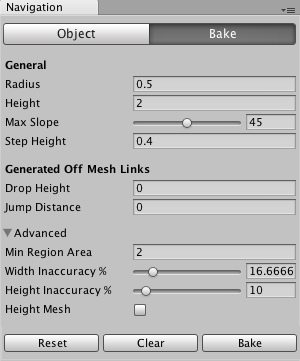
\includegraphics[width=.9\linewidth]{./pic/baking.jpg}
\end{center}
\begin{itemize}
\item Radius:具有代表性的物体半径,半径越小生成的网格面积越大。
\item Height:具有代表性的物体的高度。
\item Max Slope:斜坡的坡度。
\item Ste Height:台阶高度。
\item Drop Height:允许最大的下落距离。
\item Jump Distance:允许最大的跳跃距离。
\item Min Region Area:网格面积小于该值则不生成导航网格。
\item Width Inaccuracy:允许最大宽度的误差。
\item Height Inaccuracy:允许最大高度的误差。
\item Height Mesh:勾选后会保存高度信息,同时会消耗一些性能和存储空间。
\end{itemize}
\subsection{Nav Mesh Agent:导航组建参数面板    }
\label{sec:orgcbd518f}
\begin{itemize}
\item Radius:物体的半径
\item Speed:物体的行进最大速度
\item Acceleration:物体的行进加速度
\item Augular Speed:行进过程中转向时的角速度。
\item Stopping Distance:离目标距离还有多远时停止。
\item Auto Traverse Off Mesh Link:是否采用默认方式度过链接路径。
\item Auto Repath:在行进某些原因中断后是否重新开始寻路。
\item Height:物体的高度。
\item Base Offset:碰撞模型和实体模型之间的垂直偏移量。
\item Obstacle Avoidance Type:障碍躲避的的表现登记,None选项为不躲避障碍,另外等级越高,躲避效果越好,同时消耗的性能越多。
\item Avoidance Priority:躲避优先级。
\item NavMesh Walkable:该物体可以行进的网格层掩码。
\end{itemize}

\section{基类MonoBehaviour/自带函数以及脚本执行的生命周期}
\label{sec:org7a21080}
\begin{itemize}
\item Awake -> OnEnable -> Start ->-> FixedUpdate -> Update  -> LateUpdate ->OnGUI -> OnDisable -> OnDestroy
\end{itemize}
\subsection{MonoBehaviour的生命周期:}
\label{sec:org9d4a81f}
\begin{itemize}
\item MonoBehaviour是Unity中所有脚本的基类,如果你使用JS的话,脚本会自动继承MonoBehaviour。如果使用C\#的话,你需要显式继承MonoBehaviour。
\item 在我们使用MonoBehaviour的时候,尤其需要注意的是它有哪些可重写函数,这些可重写函数会在游戏中发生某些事件的时候被调用。我们在Unity中最常用到的几个可重写函数是这几个:
\begin{itemize}
\item Awake:当一个脚本实例被载入时Awake被调用。我们大多在这个类中完成成员变量的初始化,执行一次。
\item Start:仅在Update函数第一次被调用前调用,只执行一次。因为它是在Awake之后被调用的,我们可以把一些需要依赖Awake的变量放在Start里面初始化。同时我们还大多在这个类中执行StartCoroutine进行一些协程的触发。要注意在用C\#写脚本时,必须使用StartCoroutine开始一个协程,但是如果使用的是JavaScript,则不需要这么做。
\item Update:当MonoBehaviour启用时,其Update在每一帧被调用。
\item FixedUpdate:当MonoBehaviour启用时,其 FixedUpdate 在每一固定帧被调用。生命周期中可以被执行多次。FixedUpdate函数适合调用Rigidbody逻辑。
\item OnEnable:当对象变为可用或激活状态时此函数被调用。可执行多次,每次激活对象时对象上MonoBehaviour上脚本会调用一次。
\end{itemize}
\begin{minted}[linenos=true]{java}
gameObject.SetActive(false);// 先隐藏对象
gameObject.SetActive(true); // 显示对象
// 或
enabled = false; // 先关闭启用
enabled = true;  // 开启启用
// 都会立马会执行OnEnable函数
// 函数里适合放适配的逻辑
\end{minted}
\begin{itemize}
\item OnDisable:当对象变为不可用或非激活状态时此函数被调用。
\item OnDestroy:当MonoBehaviour将被销毁时,这个函数被调用。
\end{itemize}
\end{itemize}
\subsection{编辑器(Editor)}
\label{sec:orgfdadcb1}
\begin{itemize}
\item Reset:Reset函数被调用来初始化脚本属性当脚本第一次被附到对象上,并且在Reset命令被使用时也会调用。 
\begin{itemize}
\item 编者注:Reset是在用户点击Inspector面板上Reset按钮或者首次添加该组件时被调用。Reset最常用于在见识面板中给定一个默认值。
\end{itemize}
\end{itemize}
\subsection{第一次场景加载(First Scene Load)}
\label{sec:org68314d3}
\begin{itemize}
\item 这些函数会在一个场景开始(场景中每个物体只调用一次)时被调用。
\item Awake:这个函数总是在任何Start()函数之前一个预设被实例化之后被调用,如果一个GameObject是非激活的(inactive),在启动期间Awake函数是不会被调用的直到它是活动的(active)。
\item OnEnable:只有在对象是激活(active)状态下才会被调用,这个函数只有在object被启用(enable)后才会调用。这会发生在一个MonoBehaviour实例被创建,例如当一个关卡被加载或者一个带有脚本组件的GameObject被实例化。
\item 注意:当一个场景被添加到场景中,所有脚本上的Awake()和OnEable()函数将会被调用在Start()、Update()等它们中任何函数被调用之前。自然的,当一个物体在游戏过程中被实例化时这不能被强制执行。
\end{itemize}
\subsection{第一帧更新之前(Before the first frame update)}
\label{sec:org2c7d23b}
\begin{itemize}
\item Start:只要脚本实例被启用了Start()函数将会在Update()函数第一帧之前被调用。 
\begin{itemize}
\item 对于那些被添加到场景中的物体,所有脚本上的Start()函数将会在它们中任何的Update()函数之前被调用,自然的,当一个物体在游戏过程中被实例化时这不能被强制执行。
\end{itemize}
\end{itemize}
\subsection{在帧之间(In between frames)}
\label{sec:orgbc8a07f}
\begin{itemize}
\item OnApplicationPause:这个函数将会被调用在暂停被检测有效的在正常的帧更新之间的一帧的结束时。在OnApplicationPause被调用后将会有额外的一帧用来允许游戏显示显示图像表示在暂停状态下。
\end{itemize}
\subsection{更新顺序(Update Order)}
\label{sec:org6eadb93}
\begin{itemize}
\item 当你在跟踪游戏逻辑和状态,动画,相机位置等的时候,有几个不同的事件函数你可以使用。常见的模式是在Update()函数中执行大多数任务,但是也有其它的函数你可以使用。
\item FixedUpdate: FixedUpdate函数经常会比Update函数更频繁的被调用。它一帧会被调用多次,如果帧率低它可能不会在帧之间被调用,就算帧率是高的。所有的图形计算和更新在FixedUpdate之后会立即执行。当在FixedUpdate里执行移动计算,你并不需要Time.deltaTime乘以你的值,这是因为FixedUpdate是按真实时间,独立于帧率被调用的。
\item Update: Update每一帧都会被调用,对于帧更新它是主要的负荷函数。
\item LateUpdate:LateUpdate会在Update结束之后每一帧被调用,任何计算在Update里执行结束当LateUpdate开始时。LateUpdate常用为第三人称视角相机跟随。
\end{itemize}
\subsection{渲染(Rendering)}
\label{sec:org2b1c833}
\begin{itemize}
\item OnPreCull: 在相机剔除场景前被调用。剔除是取决于哪些物体对于摄像机是可见的,OnPreCull仅在剔除起作用之前被调用。
\item OnBecameVisible/OnBecameInvisible:当一个物体对任意摄像机变得可见/不可见时被调用。
\item OnPreRender:在摄像机开始渲染场景之前调用。
\item OnRenderObject:在指定场景渲染完成之后调用,你可以使用GL类或者Graphics.DrawMeshNow 来绘制自定义几何体在这里。
\item OnPostRender:在摄像机完成场景渲染之后调用。
\item OnRenderImage(Pro Only):在场景徐然完成之后允许屏幕图像后期处理调用。
\item OnGUI:为了响应GUI事件,每帧会被调用多次(一般最低两次)。布局Layout和Repaint事件会首先处理,接下来处理的是是通过Layout和键盘/鼠标事件对应的每个输入事件。
\item OnDrawGizmos:用于可视化的绘制一些小玩意在场景视图中。
\end{itemize}
\subsection{协同程序(Coroutines)}
\label{sec:org7866f59}
\begin{itemize}
\item 正常的协同程序更新是在Update函数返回之后运行。一个协同程序是可以暂停执行(yield)直到给出的依从指令(YieldInstruction )完成,写成的不同运用:
\item yield:在所有的Update函数都已经被调用的下一帧该协程将持续执行。
\item yield WaitForSeconds:一段指定的时间延迟之后继续执行,在所有的Update函数完成调用的那一帧之后。
\item yield WaitForFixedUpdate:所有脚本上的FixedUpdate函数已经执行调用之后持续。
\item yield WWW:在WWW下载完成之后持续。
\item yield StartCoroutine:协同程序链,将会等到MuFunc函数协程执行完成首先。
\end{itemize}
\subsection{销毁(When the Object is Destroyed)}
\label{sec:orgba0df95}
\begin{itemize}
\item OnDestory:这个函数在会在一个对象销毁前一帧调用,会在所有帧更新一个对象存在的最后一帧之后执行,对象也许会响应Object.Destroy 或一个场景关闭时被销毁。
\end{itemize}
\subsection{退出游戏(When Quitting)}
\label{sec:org157ec30}
\begin{itemize}
\item 这些函数会在你场景中所有的激活的物体上调用:
\item OnApplicationQuit:这个函数在应用退出之前的所有游戏物体上调用,在编辑器(Editor)模式中会在用户停止PlayMode时调用,在网页播放器(web player)中会在网页视图关闭时调用。
\item OnDisable:当行为变为非启用(disable)或非激活(inactive)时调用。
\end{itemize}
\subsection{官方给出的脚本中事件函数的执行顺序如下图}
\label{sec:org7bb1578}

\begin{center}
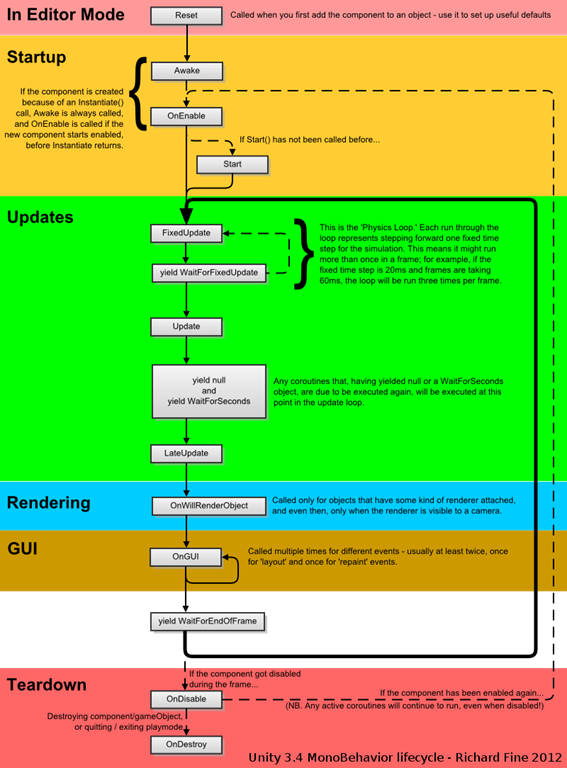
\includegraphics[width=.9\linewidth]{./pic/lfecycle.png}
\end{center}

\begin{center}
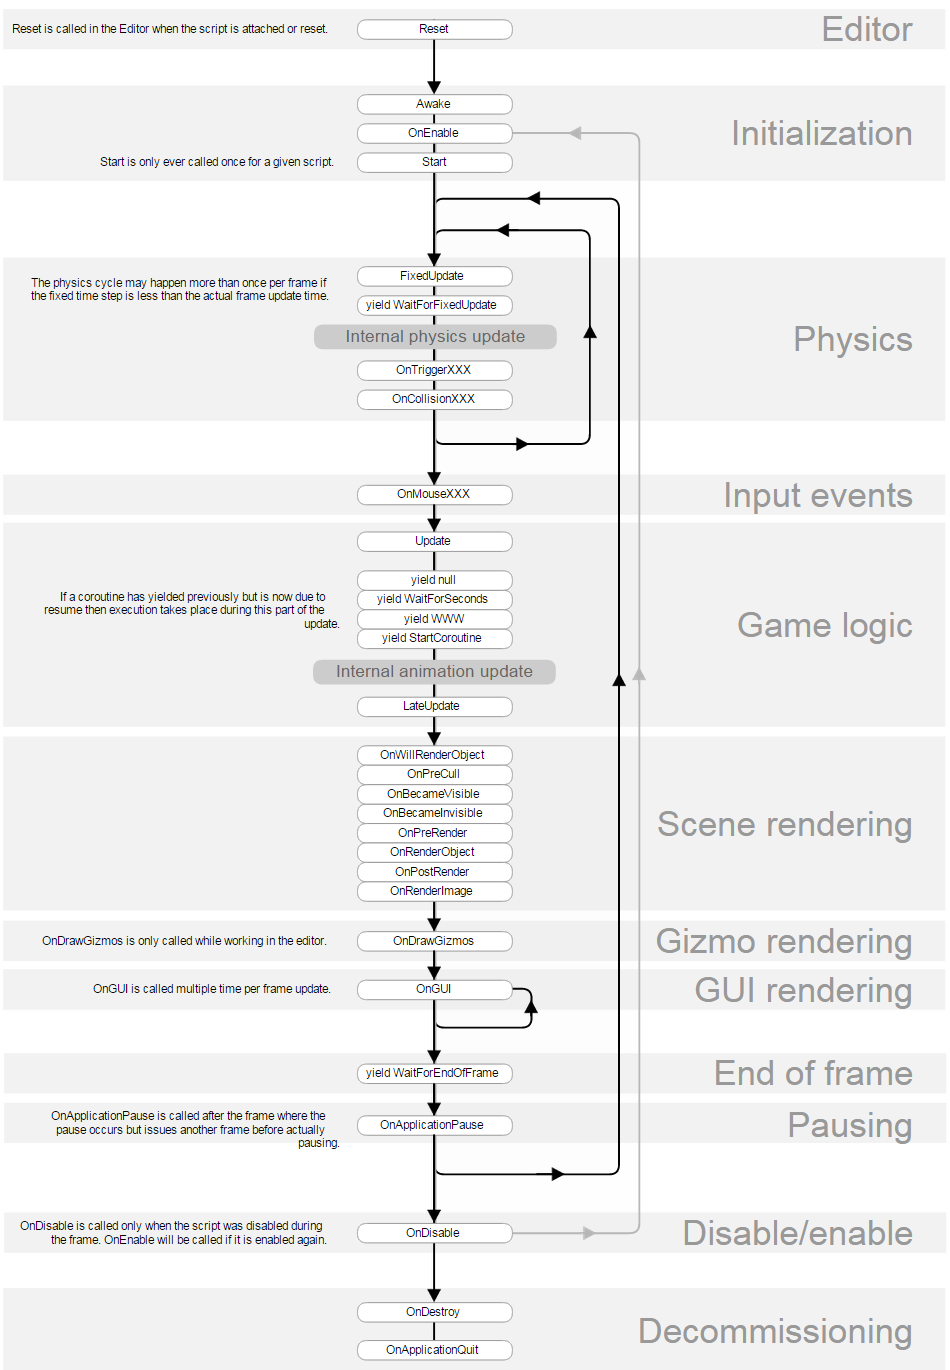
\includegraphics[width=.9\linewidth]{./pic/lifecyclefunc.png}
\end{center}

\section{Unity Study Notes}
\label{sec:orgf0b614c}
\subsection{Unity3D重要模块的类图}
\label{sec:org98ba0e8}
\begin{center}
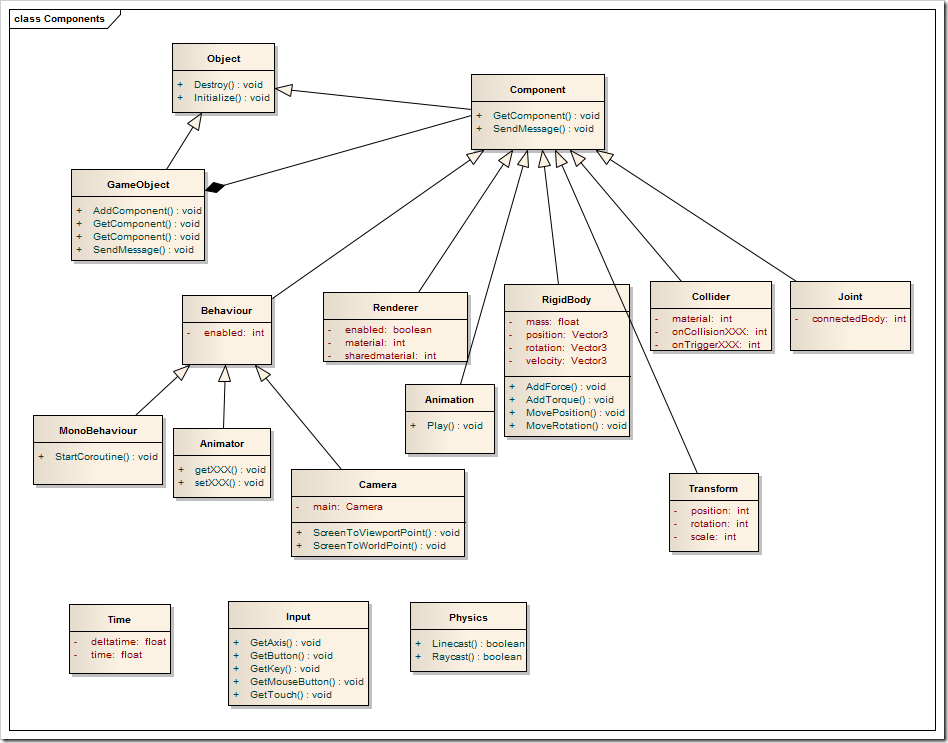
\includegraphics[width=.9\linewidth]{./pic/classes.png}
\end{center}
\subsection{GameObject和Component}
\label{sec:org40f047a}
\begin{itemize}
\item 由于Unity是一个Component-Based的游戏引擎,所以游戏中所有的物体都是一个GameObject,为了给这个GameObject附加上各种各样的属性,所以我们引入了Component这个概念。
\item GameObject是由Component组合成的,Component的生命周期和GameObject息息相关。一旦GameObject的Destroy方法,它的子对象和对应的所有Component都会被销毁,同时,我们也可以一次只销毁一个单独的Component。
\item Component有如下这些种类,我制作了一张表格来记录它们的用途:

\begin{center}
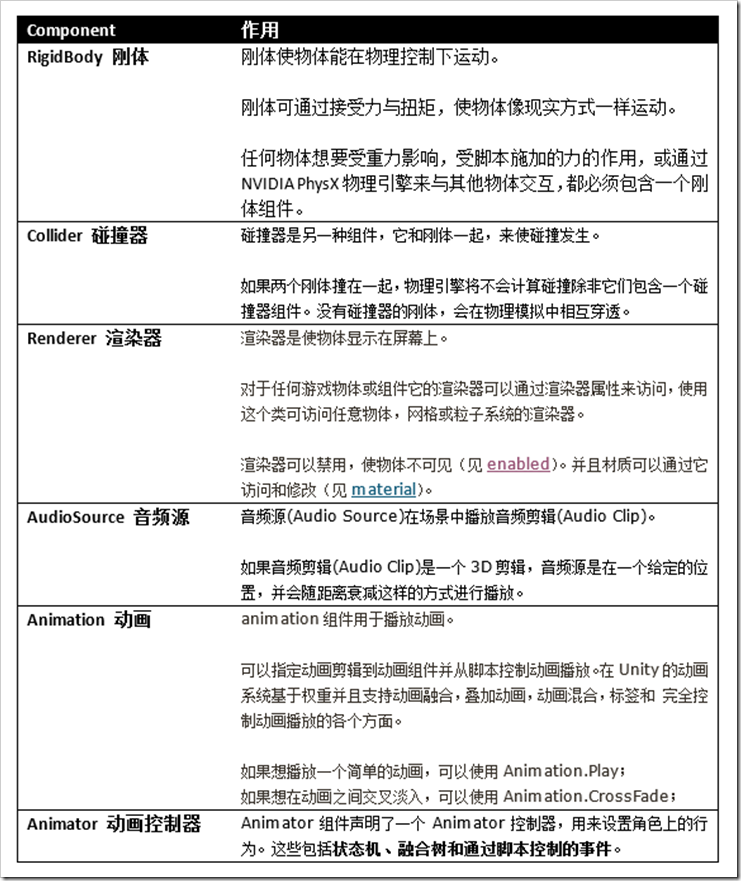
\includegraphics[width=.9\linewidth]{./pic/components.png}
\end{center}
\end{itemize}
\subsection{3D基础知识}
\label{sec:orgf74bfeb}
\subsubsection{点乘与叉乘}
\label{sec:org64d7c6c}
\begin{enumerate}
\item 点乘
\label{sec:org9370e30}
\begin{itemize}
\item S = U 点乘 V = U的模 乘以 V的模 再乘以 COS(UV之间的角度)( a dot b = |a||b|cost(theta) )
\item 这样得出来的是一个标量S,是没有方向的值。但是根据这个值与0的比较,我们可以获得U,V两标量之间的关系。
\begin{itemize}
\item 如果 = 0,那么向量 u . v 相等。
\item 如果 > 0,那么向量 u 、v 之间的夹角小于90度。
\item 如果 < 0,那么向量 u 、v 之间的夹角大于90度。
\end{itemize}
\end{itemize}

\item 叉乘
\label{sec:org8d65826}
\begin{itemize}
\item 叉积(英语:Cross product)是一种在向量空间中向量的二元运算。与点积不同,它的运算结果是一个向量而不是一个标量。两个向量的叉积写作 a * b,也称作外积(英语:Outer product)或向量积(英语:Vector product)。叉积与原来的两个向量都垂直。
\end{itemize}

\begin{center}
\includegraphics[width=.9\linewidth]{./doc/crossproduct.png}
\end{center}

\begin{minted}[linenos=true]{java}
S = U 叉乘 V 
  = [( UyVz - UzVy ),
     ( UzVx - UxVy ),
     ( UxVy - UyVx)];
\end{minted}
\begin{itemize}
\item 我们从中可以看出,我们叉乘得到的不再是一个无方向标量值。而是一个向量。那么这个向量是什么样的向量呢。
\item 我们应该去记住,两个向量叉乘得到的是一个同时垂直于这两个向量的一个新向量。
\end{itemize}
\end{enumerate}

\subsubsection{Quaternion}
\label{sec:org0d4f761}
\begin{itemize}
\item 我们用四元组来表示旋转,一个四元组包含四个分量x, y, z, w。假设一个旋转的旋转轴是axis,旋转角度是theta。那么对应的四元组q如下。
\begin{minted}[linenos=true]{java}
q.x = sin(theta / 2) * axis.x;
q.y = sin(theta / 2) * axis.y;
q.z = sin(theta / 2) * axis.z;
q.w = cos(theta / 2);
\end{minted}
\end{itemize}

\subsection{map贴图}
\label{sec:org03938ba}
\subsubsection{normalmap}
\label{sec:orgdfcd2b0}
\subsubsection{Bump Map 凹凸贴图}
\label{sec:org4b2a5d2}
\begin{itemize}
\item 

\item 

\item 

\item 

\item 

\item 

\item 

\item 

\item 
\end{itemize}

\subsection{NavMesh}
\label{sec:orgfc6a1ca}
\begin{itemize}
\item \url{http://liweizhaolili.blog.163.com/blog/static/16230744201271225812998/}
\item 

\item 
\end{itemize}
\subsection{粒子系统}
\label{sec:org5798f43}
\begin{itemize}
\item 
\end{itemize}

\subsection{references}
\label{sec:orgc112464}
\begin{itemize}
\item 入门 1-5 \url{http://www.cnblogs.com/neverdie/p/How\_To\_Learn\_Unity3D.html}
\item Unity Manual \url{http://docs.unity3d.com/Manual/index.html}
\item \url{https://unity3d.com/cn/learn}
\item \url{http://www.cnblogs.com/neverdie/}
\item \url{http://subject.manew.com/learn/index.html}
\item 摄像机 raycast 拉近与拉远 momo \url{http://www.xuanyusong.com/archives/1991}
\item 

\item 
\end{itemize}
\subsection{comments}
\label{sec:org42b5edb}
\subsection{【Unity3D基础教程】给初学者看的Unity教程(一)}
\label{sec:org39ae029}
\subsubsection{Unity 3d (just so that don't occupy a chapter)}
\label{sec:org76f0afa}
\begin{itemize}
\item 熟练者,关注Unity圣典和Unity User Manual,在这一阶段,要把在第一阶段所忽略的内容进行选择性的补充学习。
\item 进阶者,关注Unity社区,Unity Answers,Unity Wiki和知乎的Unity板块,在这一阶段,要对Unity的各种细节问题,优化,底层原理和新的技术方案都要进行思考和学习。在以上几个模块中,知乎的Unity板块尤其值得关注,干货满满而且都是中文,建议通读。看书。对知识点进行查漏补缺,我个人用的是《unity 5.x 从入门到精通》。
\item 在进阶者这一阶段,你才可以对一些中间件进行学习,具体学习什么样的Asset,还要由你的项目需求决定,不过无论如何还是推荐学习这几个Asset:Behavior Designer(AI), DoTween(Tween动画), PlayMaker(可视化编程),Shader Forge(可视化的Shader编写)和Elementals(粒子特效)。
\item 如果你还觉得不过瘾的话,就可以尝试反编译一些市面上流行的Unity3D游戏来获取代码,毕竟真实生产环境中的代码才是最值得深入研究的,在这部分我还是要推荐啪啪三国的代码,相当整洁。
\item 个人觉得就Unity学习,掌握几个很重要的点,
\begin{enumerate}
\item 基本编程语言功底,C\#、js、数据结构、算法
\item Unity资源流原理(Unity如何处理资源关系的,mate、 library、prefab之间的关系 dll如何被引用等等),基于这些关系去构建自己的资源管理结构。
\item 做好对象生命周期管理(利于管理内存、利于更加灵活结构化)
\item 善用unity文档和answer
\item 我是很不赞同去看网络上的demo来学习Unity的,Untiy的思想是可以用任意脚本对象去构建一个项目,这是非常方便非常灵活的,这是个很大的优点,然而这对于新手来说是很可怕的缺点,就像往一个容器里放入很多散落的个体,然而在项目这些个体又是项目有引用关系的,那么个体之间的偶合关系处理的不好那这就会成一个项目很大的问题。然而目前网络上的demo,大部分都是不够结构化不够框架化的初级demo。于初学者很悲催的一点是,如果一开始你从这些demo上去理解Unity,你就会进入完全基于实现的误区。很多问题都靠挂载脚本来解决,于产品级项目这样的思想是很可怕的,会严重影响产品迭代速度、管理成本以及时间成本。甚至很多教学视频往往也是把新手引入了这个误区。
\end{enumerate}
\item Model-View-Controller(MVC)是一种组合设计模式,它体现了一种关注点分离(Separation of concerns,SoC)的思想。MVC主要把逻辑层和表现层进行了解耦,将一个问题划分成了不同的关注点。增强了应用的稳定性,易修改性和易复用性。
\end{itemize}
\subsubsection{重要类及其关系}
\label{sec:orge20bf8d}
\begin{center}
\includegraphics[width=.9\linewidth]{./doc/设计类图.png}
\end{center}

\begin{center}
\includegraphics[width=.9\linewidth]{./doc/component.png}
\end{center}

\subsubsection{Input输入}
\label{sec:org88045f1}
\begin{itemize}
\item Unity支持,键盘,操纵杆和游戏手柄输入。
\item 当创建时,每个项目都具有下面的默认输入轴:
\begin{itemize}
\item Horizontal and Vertical are mapped to w, a, s, d and the arrow keys.
\item 水平和垂直被映射到w, a, s, d键和方向键
\item Fire1, Fire2, Fire3 are mapped to Control, Option (Alt), and Command, respectively.
\item Fire1, Fire2, Fire3被分别映射到Ctrl,Option(Alt)和Command键
\item Mouse X and Mouse Y are mapped to the delta of mouse movement.
\item Mouse X 和 Mouse Y被映射到鼠标移动增量
\item Window Shake X and Window Shake Y is mapped to the movement of the window.
\item Window Shake X 和 Window Shake Y 被映射到窗口的移动
\end{itemize}
\end{itemize}
\subsubsection{Time}
\label{sec:org7cb0904}
\begin{itemize}
\item Time类是Unity中的一个全局变量,它记载了和游戏相关的时间,帧数等数据。
\item Time 类包含一个非常重要的变量叫deltaTime.这个变量包含从上次调用Update 或FixedUpdate到现在的时间(根据你是放在Update函数还是FixedUpdate函数中).(另注: Update每帧调用一次)
\item 依照上面的例子,使得物体在一个匀速的速度下旋转,不依赖帧的速率,如下:
\begin{minted}[linenos=true]{java}
using UnityEngine;
using System.Collections;

public class example : MonoBehaviour {
    void Update() {
        transform.Rotate(0, 5 * Time.deltaTime, 0);
    }
}
\end{minted}
\item 当然了,在使用Time这个类的时候,我们也要记住使用各种各样的Lerp (线性插值) 函数来减少自己的工作量,在Unity3D中,Vector3,Vector2,Color等类都提供了相应的Lerp函数给我们调用。
\end{itemize}

\subsubsection{Physics和Transform}
\label{sec:org5c37cbd}
\begin{itemize}
\item Physics类是Unity重的一个工具函数类,它主要提供了Linecast和Raycast两种射线投射方式。
\begin{itemize}
\item 其中Linecast是以投射的起始位置和终止位置为参数,来判断这个投射有没有和某个Collider发生了碰撞。
\item 而Raycast则是以投射的起始位置和投射方向为参数,来判断这个投射有没有和某个Collider发生了碰撞。
\end{itemize}
\item 相应的实例可以看下面的这一段程序:
\begin{minted}[linenos=true]{java}
using UnityEngine;
using System.Collections;

public class Example : MonoBehaviour {
    void Update() {
        // 使用Raycast
        Vector3 fwd = transform.TransformDirection(Vector3.forward);
        if (Physics.Raycast(transform.position, fwd, 10))
            print("There is something in front of the object!");
    // 使用Linecast
    Transform target;
    if (!Physics.Linecast(transform.position, target.position))
        ProcessData.AndDoSomeCalculations();
    }
}
\end{minted}
\item 在Physics这个模块中,有三个Component是至关重要的,分别是RigidBody,Collision,Joint。在新的版本中,又引入了RigidBody2D,Collision2D,Joint2D这些Component来处理2D中的Physics事件。
\item 这三个类都是处理物理相关的事件的,那么它们有什么区别呢?
\begin{itemize}
\item RgidBody是作为一个受力物体而存在的,所以可以向一个RigidBody施加Force(力),Drag(阻力)。同时RigidBody还有 velocity (速度),mass(质量),position(位置),旋转(rotation)等等。
\item Collider是为了处理物理中的碰撞事件而出现的类,就像上面表格中所说的,如果没有Collider,两个RigidBody之间是无法发生碰撞的。对同一个GameObject可以绑定多个Collider构建更加复杂的碰撞体结构。
\begin{itemize}
\item Collider另外一个很值得注意的就是我们可以为Collider设置material,即Collider的物理材质。 物理材质用于调整摩擦力和碰撞单位之间的反弹效果。
\item 当发生碰撞时,会触发毁掉函数OnCollisionEnter,OnCollisionStay,OnCollisionExit等等。这几个函数与OnTriggerXXX的区别会在接下来的博客中提到。
\end{itemize}
\item Joint用于连接两个RigidBody,当Joint断掉的时候会触发OnJointBreak的回调函数。
\end{itemize}
\end{itemize}

\subsection{【Unity3D基础教程】给初学者看的Unity教程(二):所有脚本组件的基类 -- MonoBehaviour的前世今生}
\label{sec:orgda502be}
\subsubsection{引子}
\label{sec:org05fb71a}
\begin{itemize}
\item 上一次我们讲了GameObject,Compoent,Time,Input,Physics,其中Time,Input,Physics都是Unity中的全局变量。GameObject是游戏中的基本物件。GameObject是由Component组合而成的,GameObject本身必须有Transform的Component,这也加深了我们对GameObject的理解,即GameObject是游戏场景中真实存在,而且有位置的一个物件。
\item 但是我们怎么操纵这个GameObject呢?这就需要引入脚本组件了,也就是今天讲的MonoBehaviour
\end{itemize}
\subsubsection{MonoBehaviour的生命周期}
\label{sec:orgfd5e8a2}
\begin{itemize}
\item MonoBehaviour是Unity中所有脚本的基类,如果你使用JS的话,脚本会自动继承MonoBehaviour。如果使用C\#的话,你需要显式继承MonoBehaviour。
\item 在我们使用MonoBehaviour的时候,尤其需要注意的是它有哪些可重写函数,这些可重写函数会在游戏中发生某些事件的时候被调用。我们在Unity中最常用到的几个可重写函数是这几个:
\begin{itemize}
\item Awake:当一个脚本实例被载入时Awake被调用。我们大多在这个类中完成成员变量的初始化
\item Start:仅在Update函数第一次被调用前调用。因为它是在Awake之后被调用的,我们可以把一些需要依赖Awake的变量放在Start里面初始化。 同时我们还大多在这个类中执行StartCoroutine进行一些协程的触发。要注意在用C\#写脚本时,必须使用StartCoroutine开始一个协程,但是如果使用的是JavaScript,则不需要这么做。
\item Update:当MonoBehaviour启用时,其Update在每一帧被调用。
\item FixedUpdate:当MonoBehaviour启用时,其 FixedUpdate 在每一固定帧被调用。
\item OnEnable:当对象变为可用或激活状态时此函数被调用。
\item OnDisable:当对象变为不可用或非激活状态时此函数被调用。
\item OnDestroy:当MonoBehaviour将被销毁时,这个函数被调用。
\end{itemize}
\item 下面用一张图来更形象地说明一下这几个类的在MonoBehaviour的生命周期中是如何被调用的:
\end{itemize}
\begin{center}
\includegraphics[width=.9\linewidth]{./doc/monobehaviour.png}
\end{center}
\subsubsection{MonoBehaviour的那些坑}
\label{sec:org25ab120}
\begin{itemize}
\item 私有(private)和保护(protected)变量只能在专家模式中显示.属性不被序列化或显示在检视面板.
\item 不要使用命名空间(namespace)
\item 记得使用 缓存组件查找, 即在MonoBehaviour的长远方法中经常被访问的组件最好在把它当作一个私有成员变量存储起来。
\item 在游戏里经常出现需要检测敌人和我方距离的问题,这时如果要寻找所有的敌人,显然要消耗的运算量太大了,所以最好的办法是将攻击范围使用Collider表示,然后将Collider的isTrigger设置为True。最后使用OnTriggerEnter来做攻击范围内的距离检测,这样会极大提升程序性能。
\end{itemize}

\subsection{【Unity3D基础教程】给初学者看的Unity教程(三):通过制作Flappy Bird了解Native 2D中的Sprite, Animation}
\label{sec:orgac12afc}
\subsection{【Unity3D基础教程】给初学者看的Unity教程(四):通过制作Flappy Bird了解Native 2D中的Sprite, Animation}
\label{sec:org92492b5}

\subsection{【Unity3D基础教程】给初学者看的Unity教程(五):详解Unity3d中的协程(Coroutine)}
\label{sec:orgd771425}
\subsubsection{为什么需要协程}
\label{sec:org03afe12}
\begin{itemize}
\item 在游戏中有许多过程(Process)需要花费多个逻辑帧去计算。
\begin{itemize}
\item 你会遇到“密集”的流程,比如说寻路,寻路计算量非常大,所以我们通常会把它分割到不同的逻辑帧去进行计算,以免影响游戏的帧率。
\item 你会遇到“稀疏”的流程,比如说游戏中的触发器,这种触发器大多数时候什么也不做,但是一旦被调用会做非常重要的事情(比图说游戏中自动开启的门就是在门前放了一个Empty Object作为trigger,人到门前就会触发事件)。
\end{itemize}
\item 不管什么时候,如果你想创建一个能够历经多个逻辑帧的流程,但是却不使用多线程,那你就需要把一个任务来分割成多个任务,然后在下一帧继续执行这个任务。
\item 比如,A*算法是一个拥有主循环的算法,它拥有一个open list来记录它没有处理到的节点,那么我们为了不影响帧率,可以让A*算法在每个逻辑帧中只处理open list中一部分节点,来保证帧率不被影响(这种做法叫做time slicing)。
\item 再比如,我们在处理网络传输问题时,经常需要处理异步传输,需要等文件下载完毕之后再执行其他任务,一般我们使用回调来解决这个问题,但是Unity使用协程可以更加自然的解决这个问题,如下边的程序:
\begin{minted}[linenos=true]{java}
private IEnumerator Test() {  
    WWW www = new WWW(ASSEST_URL);  
    yield return www;  
    AssetBundle bundle = www.assetBundle;
}
\end{minted}
\end{itemize}

\subsubsection{协程是什么}
\label{sec:orgebc9efc}
\begin{itemize}
\item 从程序结构的角度来讲,协程是一个有限状态机,这样说可能并不是很明白,说到协程(Coroutine),我们还要提到另一样东西,那就是子例程(Subroutine),子例程一般可以指函数,函数是没有状态的,等到它return之后,它的所有局部变量就消失了,但是在协程中我们可以在一个函数里多次返回,局部变量被当作状态保存在协程函数中,直到最后一次return,协程的状态才别清除。
\item 简单来说,协程就是:你可以写一段顺序的代码,然后标明哪里需要暂停,然后在下一帧或者一段时间后,系统会继续执行这段代码。
\end{itemize}

\subsubsection{协程怎么用?}
\label{sec:org2edd002}
\begin{itemize}
\item 一个简单的C\#代码,如下:
\begin{minted}[linenos=true]{java}
IEnumerator LongComputation() {
    while(someCondition) {
        /* 做一系列的工作 */
        // 在这里暂停然后在下一帧继续执行
        yield return null;
    }
}
\end{minted}
\end{itemize}

\subsubsection{协程是怎么工作的}
\label{sec:org4ccdb03}
\begin{itemize}
\item 注意上边的代码示例,你会发现一个协程函数的返回值是IEnumerator,它是一个迭代器,你可以把它当成指向一个序列的某个节点的指针,它提供了两个重要的接口,分别是Current(返回当前指向的元素)和MoveNext()(将指针向前移动一个单位,如果移动成功,则返回true)。IEnumerator是一个interface,所以你不用担心的具体实现。
\item 通常,如果你想实现一个接口,你可以写一个类,实现成员,等等。迭代器块(iterator block)是一个方便的方式实现IEnumerator没有任何麻烦-你只是遵循一些规则,并实现IEnumerator由编译器自动生成。
\item 一个迭代器块具备如下特征:
\begin{itemize}
\item 返回IEnumerator
\item 使用yield关键字
\end{itemize}
\item 所以yield关键词是干啥的?它声明序列中的下一个值或者是一个无意义的值。如果使用yield x(x是指一个具体的对象或数值)的话,那么movenext返回为true并且current被赋值为x,如果使用yield break使得movenext()返回false。
\item 那么我举例如下,这是一个迭代器块:
\begin{minted}[linenos=true]{java}
public void Consumer() {
    foreach(int i in Integers()) {    
        Console.WriteLine(i.ToString());
    }
}
public IEnumerable<int> Integers() {
    yield return 1;
    yield return 2;
    yield return 4;
    yield return 8;
    yield return 16;
    yield return 16777216;
}
\end{minted}
\item 注意上文在迭代的过程中,你会发现,在两个yield之间的代码只有执行完毕之后,才会执行下一个yield,在Unity中,我们正是利用了这一点,我们可以写出下面这样的代码作为一个迭代器块:
\begin{minted}[linenos=true]{java}
IEnumerator TellMeASecret() {
  PlayAnimation("LeanInConspiratorially");
  while(playingAnimation)
    yield return null;
 
  Say("I stole the cookie from the cookie jar!");
  while(speaking)
    yield return null;
 
  PlayAnimation("LeanOutRelieved");
  while(playingAnimation)
    yield return null;
}
\end{minted}
\item 然后我们可以使用下文这样的客户代码,来调用上文的程序,就可以实现延时的效果。
\begin{minted}[linenos=true]{java}
IEnumerator e = TellMeASecret();
while(e.MoveNext()) { 
    // do whatever you like
}
\end{minted}
\end{itemize}

\subsubsection{协程是如何实现延时的?}
\label{sec:org63044a1}
\begin{itemize}
\item 如你所见,yield return返回的值并不一定是有意义的,如null,但是我们更感兴趣的是,如何使用这个yield return的返回值来实现一些有趣的效果。
\item Unity声明了YieldInstruction来作为所有返回值的基类,并且提供了几种常用的继承类,如WaitForSeconds(暂停一段时间继续执行),WaitForEndOfFrame(暂停到下一帧继续执行)等等。更巧妙的是yield 也可以返回一个Coroutine真身,Coroutine A返回一个Coroutine B本身的时候,即等到B做完了再执行A。下面有详细说明:
\item Normal coroutine updates are run after the Update function returns. A coroutine is a function that can suspend its execution (yield) until the given YieldInstruction finishes. Different uses of Coroutines:
\begin{itemize}
\item yield; The coroutine will continue after all Update functions have been called on the next frame.
\item yield WaitForSeconds(2); Continue after a specified time delay, after all Update functions have been called for the frame
\item yield WaitForFixedUpdate(); Continue after all FixedUpdate has been called on all scripts
\item yield WWW Continue after a WWW download has completed.
\item yield StartCoroutine(MyFunc); Chains the coroutine, and will wait for the MyFunc coroutine to complete first.
\end{itemize}
\item 实现延时的关键代码是在StartCoroutine里面,以为笔者也没有见过Unity的源码,那么我只能猜想StartCoroutine这个函数的内部构造应该是这样的:
\begin{minted}[linenos=true]{java}
List<IEnumerator> unblockedCoroutines;
List<IEnumerator> shouldRunNextFrame;
List<IEnumerator> shouldRunAtEndOfFrame;
SortedList<float, IEnumerator> shouldRunAfterTimes;

foreach(IEnumerator coroutine in unblockedCoroutines) {
    if(!coroutine.MoveNext())
        // This coroutine has finished
        continue;
 
    if(!coroutine.Current is YieldInstruction) {    
        // This coroutine yielded null, or some other value we don't understand; run it next frame.
        shouldRunNextFrame.Add(coroutine);
        continue;
    }
 
    if(coroutine.Current is WaitForSeconds) {    
        WaitForSeconds wait = (WaitForSeconds)coroutine.Current;
        shouldRunAfterTimes.Add(Time.time + wait.duration, coroutine);
    } else if(coroutine.Current is WaitForEndOfFrame) {    
        shouldRunAtEndOfFrame.Add(coroutine);
    } else /* similar stuff for other YieldInstruction subtypes */
}
unblockedCoroutines = shouldRunNextFrame;
\end{minted}
\item 当然了,我们还可以为YieldInstruction添加各种的子类,比如一个很容易想到的就是yield return new WaitForNotification(“GameOver”)来等待某个消息的触发,关于Unity的消息机制可以参考这篇文章:【Unity3D技巧】在Unity中使用事件/委托机制(event/delegate)进行GameObject之间的通信 (二) : 引入中间层NotificationCenter。
\end{itemize}

\subsubsection{还有些更好玩的?}
\label{sec:org190c52e}
\begin{itemize}
\item 第一个有趣的地方是,yield return可以返回任意YieldInstruction,所以我们可以在这里加上一些条件判断:
\begin{minted}[linenos=true]{java}
YieldInstruction y;

if (something)
    y = null;
else if (somethingElse)
    y = new WaitForEndOfFrame();
else
    y = new WaitForSeconds(1.0f);

yield return y;
\end{minted}
\item 第二个,由于一个协程只是一个迭代器块而已,所以你也可以自己遍历它,这在一些场景下很有用,例如在对协程是否执行加上条件判断的时候:
\begin{minted}[linenos=true]{java}
IEnumerator DoSomething() {
  /* ... */
}
 
IEnumerator DoSomethingUnlessInterrupted(){
    IEnumerator e = DoSomething();
    bool interrupted = false;
    while(!interrupted) {  
        e.MoveNext();
        yield return e.Current;
        interrupted = HasBeenInterrupted();
    }
}
\end{minted}
\item 第三个,由于协程可以yield协程,所以我们可以自己创建一个协程函数,如下:
\begin{minted}[linenos=true]{java}
IEnumerator UntilTrueCoroutine(Func fn) {
    while (!fn()) 
        yield return null;
}
 
Coroutine UntilTrue(Func fn) {
    return StartCoroutine(UntilTrueCoroutine(fn));
}
 
IEnumerator SomeTask() {
    /* ... */
    yield return UntilTrue(() => _lives < 3);
    /* ... */
}
\end{minted}
\end{itemize}

\subsection{【Unity3D基础教程】给初学者看的Unity教程(六):理解unity的新GUI系统(UGUI)}
\label{sec:org85dcd17}
\begin{itemize}
\item UGUI是Unity在4.6中引入的新的GUI系统,与传统的中间件NGUI相比,这套新GUI系统有几个核心亮点:
\begin{itemize}
\item 放弃了Atlas的概念,使用Packing Tag的方式来进行图集的规划
\item 放弃了depth来确定UI显示层级的概念,使用Hierarchy的SiblingIndex来确定先是层级
\item 使用RectTransform来代替以前NGUI中的UIAnchor,分辨率适配更加简单
\item 使用LayoutGroup代替以前的NGUI中的Grid,实现了更灵活的布局
\end{itemize}
\item UGUI的类继承结构还是挺复杂的,如果你想对此有了解的话,可以参考我的两个类图:
\begin{itemize}
\item Unity GUI 链接:UnityEngine.UI系统基础类架构图 \url{https://www.processon.com/view/link/55421d91e4b01376faa9d6fb}
\item Unity Event System 链接:UnityEngine Event \& EventSystem系统架构图 \url{https://www.processon.com/view/55421efce4b01376faa9dbfe}
\end{itemize}
\end{itemize}

\subsection{【Unity3D基础教程】给初学者看的Unity教程(七):在unity中构建健壮的单例模式(Singleton)}
\label{sec:orgd657133}
\subsubsection{为什么需要单例模式}
\label{sec:org3f59f1e}
\begin{itemize}
\item 游戏中需要单例有以下几个原因:
\begin{itemize}
\item 我们需要在游戏开始前和结束前做一些操作,比如网络的链接和断开,资源的加载和卸载,我们一般会把这部分逻辑放在单例里。
\item 单例可以控制初始化和销毁顺序,而静态变量和场景中的GameObject都无法控制自己的创建和销毁顺序,这样就会造成很多潜在的问题。
\item Unity3D的GameObject需要动态创建。而不是固定在场景里,我们需要使用单例来创建GameObject。
\item Unity3D的场景中的各个GameObject需要从单例中存取数据。
\end{itemize}
\end{itemize}
\subsubsection{单例的设计原则}
\label{sec:org87b119a}
\begin{itemize}
\item 在设计单例的时候,我并不建议采取延迟初始化的方案,正如云风所说: \textbf{对于单件的处理,采用静态对象和惰性初始化的方案,简直就是 C++ 程序员的陋习。Double Checked Locking is broken,相信很多人都读过了。过于依赖语法糖,通常就会造成这种结果。其实让程序有明显的初始化和退出阶段,是很容易被规划出来的。把单件(singleton) 的处理放在正确的时机,以正确的次序来处理并非难事。}
\item 我们应该在程序某处明确定义单例是否被初始化,在初始化执行完毕后再执行正常的游戏逻辑
\begin{itemize}
\item 尽量避免多线程创建单例带来的复杂性
\item 在某处定义了一定的初始化顺序后,可以在游戏结束的时候按照相反的顺序销毁这些单例
\end{itemize}
\end{itemize}
\subsubsection{设计单例的基类}
\label{sec:org502d5a5}
\begin{itemize}
\item 在Unity中,我们需要一个基类来为所有单例的操作提供统一的接口,同时,我们还要让所有单例继承MonoBehaviour,只有这样才能让单例自由使用协程这一特性。
\item 基类设计如下,
\begin{minted}[linenos=true]{java}
using System;
using UnityEngine;

namespace MiniWeChat {
    [RequireComponent(typeof(GameRoot))]

    public class Singleton<T> : MonoBehaviour where T : Singleton<T> {    
        private static T _instance;

        public static T GetInstance() {        
            return _instance;
        }

        public void SetInstance(T t) {        
            if (_instance == null) {            
                _instance = t;
            }
        }

        public virtual void Init() {        
            return;
        }

        public virtual void Release() {        
            return;
        }
    }
}
\end{minted}
\end{itemize}
\subsubsection{设计单例的管理类}
\label{sec:org03ee964}
\begin{itemize}
\item 除了设计基类之外, 还需要设计一个让所有基类初始化和销毁的类,我们把这个类叫做GameRoot,并且把它绑定在一个名为GameRoot的GameObject上,并且把这个GameObject放在游戏进入的Main场景中。
\item GameRoot类设计如下,
\begin{minted}[linenos=true]{java}
namespace MiniWeChat {
    public class GameRoot : MonoBehaviour {
        private static GameObject _rootObj;
        private static List<Action> _singletonReleaseList = new List<Action>();

        public void Awake() {        
            _rootObj = gameObject;
            GameObject.DontDestroyOnLoad(_rootObj);
            StartCoroutine(InitSingletons());
        }

        /// <summary>
        /// 在这里进行所有单例的销毁
        /// </summary>
        public void OnApplicationQuit() {        
            for (int i = _singletonReleaseList.Count - 1; i >= 0; i--) {            
                _singletonReleaseList[i]();
            }
        }

        /// <summary>
        /// 在这里进行所有单例的初始化
        /// </summary>
        /// <returns></returns>
        private IEnumerator InitSingletons() {        
            yield return null;
            // Init Singletons
        }

        private static void AddSingleton<T>() where T : Singleton<T> {        
            if (_rootObj.GetComponent<T>() == null) {            
                T t = _rootObj.AddComponent<T>();
                t.SetInstance(t);
                t.Init();
                singletonReleaseList.Add(delegate() {                
                        t.Release();
                    });
            }
        }

        public static T GetSingleton<T>() where T : Singleton<T> {        
            T t = _rootObj.GetComponent<T>();
            if (t == null) {            
                AddSingleton<T>();
            }
            return t;
        }
    }
}
\end{minted}
\end{itemize}
\subsubsection{如何拓展新的单例}
\label{sec:org12ddf7a}
\begin{itemize}
\item 有了以上两个类之后,当我们需要新创建一个类的时候,就可以继承Singleton<T>来创建新的单例,重写Init和Release方法,同时在GameRoot的InitSingleton方法的适当顺序执行AddSingleton<T>方法即可。
\end{itemize}


\subsection{场景视图(Scene View)导航}
\label{sec:org53c21b7}
场景视图 (Scene View) 是你的交互式沙箱。你可以使用场景视图 (Scene View) 选择和放置环境、玩家、相机、敌人和所有其他游戏对象 (GameObjects)。

在场景视图 (Scene View) 中调动和操纵对象是 Unity 最重要的一些功能,因此,能够迅速使用它们至关重要。

场景视图 (Scene View) 有一个导航控件集,可帮助你快速高效地四处移动。

\subsubsection{上下左右箭头键}
\label{sec:orgf2f5e52}

您可以使用箭头键 (Arrow Keys) 在场景中四处移动,就像“走路”穿过一样。向上和向下箭头在相机面向的方向向前或向后移动相机。

左右箭头横向平移视图。按住 Shift 键和一个箭头键,可更快地移动。

\subsubsection{使用手形工具}
\label{sec:orgee5c0a8}

你还可以发现手形工具 (Hand Tool)(快捷键:Q)的功用,特别是使用单键鼠标时。选择手形工具 (Hand tool) 后:

\begin{center}
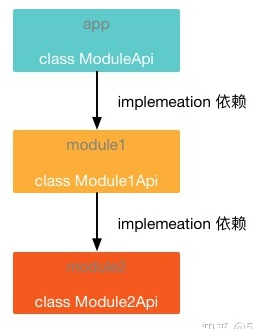
\includegraphics[width=.9\linewidth]{./pic/1.png}
\end{center}

场景视图 (Scene View) 的右上角是场景小图示 (Scene Gizmo),显示场景相机 (Scene Camera) 的当前定位,让你快速改变视角。

按住 Shift 键可提高移动和缩放的速率。

\subsubsection{漫游模式}
\label{sec:orge7ebcba}

漫游模式可让您像许多第一人称视角游戏一样来浏览场景视图 (Scene View)。

单击并按住鼠标右键进入漫游模式。

现在您可以使用鼠标将视图四处移动,使用 WASD 键向前后左右移动,使用 Q 和 E 键向上或向下移动。

按住 Shift 键可移动得更快。

漫游模式专为透视图模式而设计。在等距模式中,按住鼠标右键并移动鼠标,则会旋转相机。

\subsubsection{场景小图示(Scene Gizmo)}
\label{sec:orgda37a06}

场景视图 (Scene View) 右上角是场景小图示 (Scene Gizmo),它显示了场景视图相机 (Scene View Camera) 当前视角方向,可让你快速修改视角。

\begin{center}
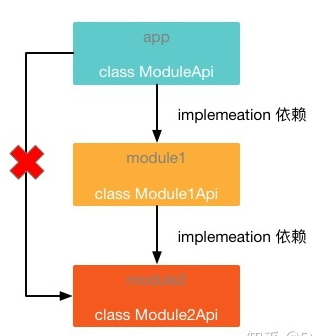
\includegraphics[width=.9\linewidth]{./pic/2.png}
\end{center}
小图示(Gizmo)的每个彩色“支脚”代表一根几何轴。

你可以点击任何方向杆,将场景视图相机 (Scene View Camera) 更改为该方向。点击场景小图示(Scene Gizmo)的中央或其下方的文本,可在等距模式和透视图模式之间切换。

你也可以常常按下 Shift 键并点击场景小图示 (Scene Gizmo) 的中央,以获得“好”的透视图,其查看场景的视角位于侧面略上方。

\subsection{定位游戏对象(GameObjects)}
\label{sec:org54a3b1d}
构建游戏时,会在游戏世界中放置许多不同的对象。此时,使用工具栏 (Toolbar) 中的转换工具 (Transform Tools),可转换、旋转及缩放单个游戏对象。

每个游戏对象的周围都有相应的小图示(Gizmo)。可使用鼠标操作任何(Gizmo)轴来修改游戏对象 (GameObjects) 的转换组件 (Transform Component),也可以在检视器 (Inspector) 中转换组件 (Transform Component) 的数字字段中直接输入值。

\begin{center}
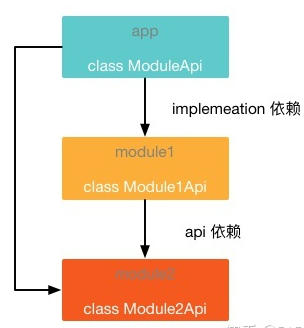
\includegraphics[width=.9\linewidth]{./pic/3.png}
\end{center}

\subsubsection{聚焦游戏对象}
\label{sec:orgcb1d6d0}

先将场景视图的相机 (Scene View Camera) 焦距一个对象,或者在层级视图中选择一个游戏对象 (GameObject),然后再将鼠移到场景视图上操纵该对象,此时视图将以对象为中心移动,这点非常有用。

选择任何游戏对象 (GameObject) 并按 F 键,这样场景视图 (Scene View) 和枢轴点会以所选对象为中心,该操作称为“框选 (Frame Selection)”。

\subsubsection{移动、旋转和缩放}
\label{sec:org11a738b}

移动、旋转和缩放是场景视图 (Scene View) 导航中的关键操作,因此,Unity 提供了几个备选方法,以在执行时提供最大方便。

以下是对一些要点的概述:

按住鼠标右键进入漫游 (Flythrough) 模式。

用鼠标和方向键(向上和向下要加上 Q 和 E 键)进入第一视角视图导航。

选择任何游戏对象 (GameObject) 并按 F 键。这将确定所选对象在场景视图的中心位置及轴点。

使用箭头键在 X/Z 平面上移动。

按住 Alt 键和鼠标左键拖动,使相机围绕当前轴点旋转。

按住 Alt 键和鼠标滚轮拖动,拖动场景视图 (Scene View) 相机。

按住 Alt 键和鼠标右键拖动,缩放场景视图 (Scene View)。此效果与滚动鼠标滚轮的效果相同。

点击并拖动小图示 (Gizmo) 中心,以同时在所有轴上操纵对象。

在转换 (Translate) 小图示的中心有三个小正方形,可用来在相同平面(即可同时移动两个轴,第三个轴保持不动)拖动对象。

如果你有一个三键鼠标,则可以点击鼠标中键来调整最后调整的轴(该轴变成黄色),而无需直接点击该轴。

使用缩放工具时要小心,因为非统一缩放,可能会导致子对象的缩放比例失衡。

\subsubsection{小图示显示切换器 (Gizmo Display Toggles)}
\label{sec:org9746a85}

小图示显示切换器 (Gizmo Display Toggles) 用来定义任何变换小图示 (Transform Gizmo) 的位置。

\begin{center}
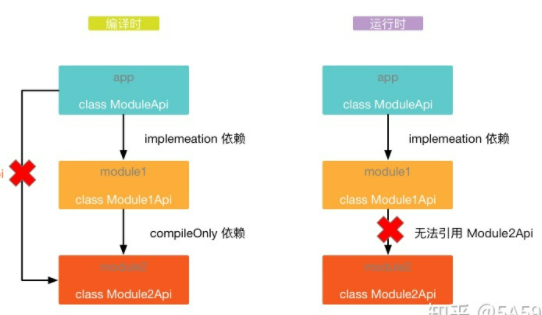
\includegraphics[width=.9\linewidth]{./pic/4.png}
\end{center}
可使用它在不同视图模式中查看场景:纹理、线框、RGB、夸张等等。还可以看(听)场景视图 (Scene View) 中的游戏照明、游戏元素及声音。

定位时,居中 (Center) 将小图示 (Gizmo) 定位在对象范围的中心。枢轴 (Pivot) 将小图示 (Gizmo) 定位在网格 (Mesh) 的实际枢轴点。

旋转时,局部 (Local) 将相对于对象的旋转保持小图示 (Gizmo) 的旋转。全局 (Global) 强制小图示 (Gizmo) 为世界空间的方向。

\subsubsection{单位对齐}
\label{sec:org32fc269}

使用转换工具 (Translate Too) 拖动任何小工具轴 (Gizmo Axis) 时,你可以按住控制键,以对齐设置 (Snap Settings) 中定义的增量。

你可以使用菜单编辑->对齐设置\ldots{}更改单位对齐所用的单位距离:

\begin{center}
\includegraphics[width=.9\linewidth]{./pic/5.png}
\end{center}

\subsubsection{表面对齐}
\label{sec:orgb0ed2a5}

使用转换工具 (Translate Too) 在中心拖动时,可以按住 Shift 键,这可将对象与任何碰撞体 (Collider) 的交叉点对齐。使对象精确定位变得更迅速。

\subsubsection{查看旋转}
\label{sec:orgadd4fd8}

使用旋转工具 (Rotate Tool) 时,可以按住 Shift 将对象朝向任何碰撞体 (Collider) 表面上的一点旋转。这可使对象相对于另一个对象的定向变得简单。

\subsubsection{顶点对齐}
\label{sec:orgc7c2142}

你可以使用一个称为顶点对齐 (Vertex Snapping) 的功能来轻松组装你的游戏世界。该功能可以让你取给定网格的任何顶点,然后用鼠标将该顶点放到你所选的任何其他网格的任何顶点上。使用该功能可以快速地组装你的游戏世界。例如,你可以在高精度竞速游戏中放置赛道,在网格的顶点添加动力道具。

\begin{center}
\includegraphics[width=.9\linewidth]{./pic/6.png}
\end{center}
使用顶点对齐 (Vertex Snapping) 组装赛道。

在 Unity 中使用顶点对齐非常简单,只需按照以下步骤操作:

\begin{enumerate}
\item 选择您要操纵的网格,确保变换工具 (Transform Tool) 处于活动状态。

\item 长 按 V 键以激活顶点对齐模式。

\item 将光标移到您想用作枢轴点的网格的顶点上。

\item 光标在想要的顶点上时按住鼠标左键,然后将网格拖到另一个网格的任何其他顶点旁边。

\item 对结果满意时,松开鼠标按键和 V 键。

\item Shift-V 用来切换该功能。
\end{enumerate}

您可以将顶点与顶点对齐、顶点与表面对齐、枢轴与顶点对齐。

\subsection{视图模式}
\label{sec:org9c3fbdd}
场景视图 (Scene View) 控制条可让您选择查看场景的各种选项及控制是否启用灯光和音频。这些控制只影响开发过程中的场景视图,对构建的游戏无影响。

\begin{center}
\includegraphics[width=.9\linewidth]{./pic/7.png}
\end{center}
\subsubsection{绘图模式 (Draw Mode)}
\label{sec:org77d2b5e}

第一个下拉菜单选择哪种绘图模式 (Draw Mode) 将用来描绘场景。

\begin{center}
\includegraphics[width=.9\linewidth]{./pic/8.png}
\end{center}
纹理:显示表面及其可见纹理。

线框:用线框绘制网格。

纹理-线框:显示带纹理且有线框覆盖的网格。

渲染路径:使用颜色代码显示每个对象的渲染路径:绿色表示延时光照、黄色表示正向渲染,红色表示顶点光明。

光照贴图分辨率:在场景上覆盖棋盘格以显示光照贴图的分辨率。

\subsubsection{渲染模式 (Render Mode)}
\label{sec:org89f5365}

下一个下拉菜单选择四种渲染模式 (Render Modes) 的哪种模式用于渲染场景。

\begin{center}
\includegraphics[width=.9\linewidth]{./pic/9.png}
\end{center}

RGB:渲染具有正常颜色的对象的场景。

Alpha:用 alpha 渲染颜色。

过度绘制(Overdraw):将对象作为透明的“剪影”渲染。透明颜色累加,这样很容易就可以找出一个对象绘制在另一个对象上的位置。

Mipmap:使用颜色代码显示理想的纹理尺寸:红色表示纹理大于所需尺寸(在当前距离和分辨率下);蓝色表示纹理可以更大。当然,理想的纹理尺寸取决于游戏运行时的分辨率及相机可以离特定表面多近。

\subsubsection{场景照明、游戏覆盖和试听模式}
\label{sec:org7d0af14}

下拉菜单的右侧有三个按钮,可控制场景表示的其他方面。

\begin{center}
\includegraphics[width=.9\linewidth]{./pic/10.png}
\end{center}
第一个按钮确定是否使用默认光照方案或实际添加到场景中的灯光来照亮视图。默认灯光方案初始时使用,但当添加第一个灯光时会自动更改。第二个按钮控制是否在场景视图中渲染天空盒和 GUI 元素,也显示和隐藏布局网格。第三个按钮开启/关闭场景中的音频源。

\subsection{小图示和图标显示控制}
\label{sec:org6335055}
小图示和图标有几个显示选项,可以用来在开发过程中减少混乱和改善场景的视觉清晰度。

\subsubsection{图标选择器 (Icon Selector)}
\label{sec:orgdf111bf}

使用图标选择器 (Icon Selector),可以轻松为游戏对象 (GameObjects) 和脚本设置自定义图标,这些图标将在场景视图 (Scene View) 和检视器 (Inspector) 中使用。要更改一个游戏对象 (GameObject) 的图标,只需在检视器 (Inspector) 中点击其图标。可用类似方法更改脚本资源的图标。在图标选择器 (Icon Selector) 中,标签图标 (Label Icon) 是一种特殊的图标。这类图标将在场景视图 (Scene View) 中作为文本标签显示,使用游戏对象 (GameObject) 的名称。内置组件 (Components) 的图标不能更改。

注意:一个资源的图标更改后,该资源将标记为“已修改”,因此由版本控制系统 (Revision Control Systems) 取回。

下面的图演示如何为游戏对象 (GameObject) 选择一个图标:

\begin{center}
\includegraphics[width=.9\linewidth]{./pic/11.png}
\end{center}

下面的图演示如何为脚本选择一个图标:

\begin{center}
\includegraphics[width=.9\linewidth]{./pic/12.png}
\end{center}
\subsubsection{显示和隐藏图标与小图示}
\label{sec:orga3ef069}

单独组件的小图示的可见性取决于组件在检视器中是否被展开或折叠(即折叠的组件不可见)。然而,您可以使用小图示 (Gizmos) 下拉菜单同时展开或折叠给定类型的每个组件。当场景中有大量小图示和图标时,这是减少视觉混乱的有效方法。

要显示当前小图示和图标的状态,单击场景 (Scene) 或游戏视图 (Game View) 控制条中的小图示 (Gizmos)。这里的切换用来设置哪种图标和小图示可见。

注意,脚本 (Scripts) 部分显示的脚本为拥有自定义图标或让 OnDrawGizmos () 或 OnDrawGizmosSelected () 函数执行的脚本。

\begin{center}
\includegraphics[width=.9\linewidth]{./pic/13.png}
\end{center}

小图示 (Gizmos) 下拉菜单,显示图标和小图示的可见状态

图标缩放 (Icon Scaling) 滑动条可以用来调节图标在场景中显示的大小。滑动条在最右端时,图标常常按实际尺寸画出。否则,图标将会根据其距场景视图相机的距离来缩放(尽管显示尺寸设有上限,以避免屏幕混乱)。

\subsection{iOS}
\label{sec:org3c8c8ae}
\begin{itemize}
\item \url{http://www.jianshu.com/p/8472ba0f2bb6}
\item \url{https://github.com/qinjx/30min\_guides/blob/master/ios.md} iOS开发60分钟入门
\item \url{http://blog.startry.com/2015/07/24/iOS\_EnvWithXcconfig/} iOS开发必备 - 环境变量配置(Debug \& Release)
\item \url{https://www.zhihu.com/question/22000647} 零基础如何学习 iOS 开发?
\item \url{https://github.com/Aufree/trip-to-iOS} iOS 学习资料整理
\item 

\item 

\item 

\item 

\item 

\item 
\end{itemize}
\subsection{Unity动画}
\label{sec:org4c0836e}
\subsubsection{shader}
\label{sec:org6fa7ba2}
\begin{itemize}
\item \url{http://www.jianshu.com/p/7b9498e58659} Unity ShaderLab学习总结
\item 

\item 

\item 

\item 

\item 

\item 

\item 

\item 

\item 


\item \url{http://www.360doc.com/content/13/0225/17/10941785\_267831975.shtml}
\item 用好Lua+Unity,让性能飞起来—LuaJIT性能坑详解 \url{https://zhuanlan.zhihu.com/p/26528101}
\item 

\item 

\item 

\item 

\item 

\item 

\item 

\item 
\end{itemize}

\section{Unity C\# Functions code practice}
\label{sec:orgc4fa09a}

\begin{minted}[linenos=true]{csharp}
using UnityEngine;
using System.Collections;

public class ActiveObjects : MonoBehaviour {

    // bgn Physics
    
    // rigidbody.AddForce(Vector3 direction & magnitude, [optional]Mode of force being used); 
    // ForceMode default to ForceMode.Force
    void OnMouseDown() {
        // AddForce() can be used in FixedUpdate() to apply a constant force
        // 4 ForceModes: Acceleration, Force, Impulse, VelocityChange
        // Acceleration & VelocityChange are NOT affected by mass
        // Force & Impulse are affected by mass
        rigidbody.AddForce(-transform.forward * 1000, ForceMode.Force);
        rigidbody.useGravity = true;
    }
    
    // rigidbody.AddTorque(Vector3 torque, ForceMode mode);
    // rigidbody.AddTorque(Vector3 as axis to apply torque around, [optional]Type of Force to apply);
    // 4 ForceModes: Acceleration, Force, Impulse, VelocityChange
    // Acceleration & VelocityChange are NOT affected by mass
    // Force & Impulse are affected by mass
    // AddTorque() is significantly affected by Angular drag, 
    //     if Angular drag is increased, it will make difficult for gameObject to torque
    public float amount = 50f;
    void FixedUpdate() {
        float h = Input.GetAxis("Horizontal") * amount * Time.deltaTime;
        float v = Input.GetAxis("Vertical") * amount * Time.deltaTime;
        rigidbody.AddTorque(transform.up * h, ForceMode.);
        rigidbody.AddTorque(transform.right * v);
    }
    
    // bgn Scripts
    public GameObject myObject;
    //int [] myInt = new int[5];
    int [] myInt = new int[] {1, 2, 3, 4, 5}; // default is private for C3, public for javascript
    public GameObject players;
    void Start() {
        Debug.Log("Active Self: " + myObject.activeSelf);
        Debug.Log("myObject.activeInHierarchy: " + myObject.activeInHierarchy);
        gameObject.SetActive(false);

        myInt[0] = 12;

        players = GameObject.FindGameObjectsWithTag("Player");
        for (int i = 0; i < players.Length; i++) {
            Debug.Log("Player number " + i + " is named " + players[i].name);
        }
    }

    public float speed = 8f;
    public float countdown = 3f;
    void Update() {
        countdown -= Time.deltaTime;
        if (countdown <= 0.0f) 
            light.enabled = true;
        if (Input.GetKey(KeyCode.RightArrow)) 
            transform.position += new Vector3(speed * Time.deltaTime, 0f, 0f);
    }

    public GameObject other;
    void Update() {
        if (Input.GetKey(KeyCode.Space)) {
            // Destory(gameObject, delayTime);
            // remove entire gameObject
            Destroy(other, 3); // 3 second delayTime
            // remove components
            Destroy(gameObject.GetComponent<MeshRenderer>());
         }
    }
    // Activate Deactivate
    void Update() {
        if (Input.GetKey(KeyCode.Space)) 
            myLight.enabled = !myLight.enabled;
    }

    public GameObject otherGameObject;
    private AnotherScript anotherScript;
    private YetAnotherScript yetAnotherScript;
    private BoxCollider boxCol;
    void Awake() {
        anotherScript = GetComponent<AnotherScript>();
        yetAnotherScript = otherGameObject.GetComponent<YetAnotherScript>();
        boxCol = otherGameObject.GetComponent<BoxCollider>();
    }
    void Start() {
        boxCol.size = new Vector3(3, 3, 3);
    }

    private Vector3 newPosition;
    private float newIntensity;
    public float smooth = 2;
    void Awake() {
        newIntensity = light.intensity;
    }
    void Update() {
        PositionChanging();
        IntensityChanging();
    }
    void PositionChanging() {
        Vector3 positionA = new Vector3(-5, 3, 0);
        Vector3 positionB = new Vector3(5, 3, 0);
        if (Input.GetKeyDown(KeyCode.Q)) 
            newPosition = positionA;
        if (Input.GetKeyDown(KeyCode.E)) 
            newPosition = positionB;
        // Vector3.Lerp(from Vector3, to Vector3, time float)
        transform.position = Vector3.Lerp(transform.position, newPosition, time.deltaTime * smooth);
    }
    void IntensityChanging() {
        float intensityA = 0.5f;
        float intensityB = 5f;
        if (Input.GetKeyDown(KeyCode.A)) 
            newIntensity = intensityA;
        if (Input.GetKeyDown(KeyCode.D)) 
            newIntensity = intensityB;
        // Mathf.Lerp(from float, to float, time float)
        light.intensity = Mathf.Lerp(light.intensity, newIntensity, Time.deltaTime * smooth);

        // Similarly, Color.Lerp(from Color, to Color, time float)
        light.color = Color.Lerp(light.color, newColor, Time.deltaTime * smooth);
    }

    void Update(){
        if (Input.GetKeyDown(KeyCode.R)) 
            gameObject.renderer.material.color = Color.red;
    }

    public float speed = 10f;
    void Update(){
        // transform.Rotate(Axis around which to rotate, amount to rotate by)
        transform.Rotate(Vector3.up, speed * Time.deltaTime); // (0, 1, 0)
        if (Input.GetKey(KeyCode.UpArrow)) 
            transform.Translate(Vector3.forward * speed * Time.deltaTime); // (0, 1, 0)
        if (Input.GetKey(KeyCode.DownArrow)) 
            transform.Translate(-Vector3.forward * speed * Time.deltaTime); // (0, 1, 0)
    }

    // VectorA: (x, y, z)
    // VectorB: (x, y, z)
    // Vector3.Dot(VectorA, VectorB)  // Unity function
    // (Ax * Bx) + (Ay * By)+ (Az * Bz) = Dot Product

    // Cross product, L于原来的两个向量
    // Vector3.Cross(VectorA, VectorB) // Unity function
}
\end{minted}
\section{[Unity]面试题整理100题}
\label{sec:org86a3d25}
\begin{itemize}
\item \url{http://gad.qq.com/article/detail/18272}
\item \url{http://gad.qq.com/article/detail/20995} 100题
\end{itemize}
\subsection{相机}
\label{sec:org3094c48}
\subsubsection{移动相机动作在哪个函数里,为什么在这个函数里?}
\label{sec:org46a9dd6}
\begin{itemize}
\item LateUpdate,是在所有的Update结束后才调用,比较适合用于命令脚本的执行。官网上例子是摄像机的跟随,都是所有的Update操作完才进行摄像机的跟进,不然就有可能出现摄像机已经推进了,但是视角里还未有角色的空帧出现。
\end{itemize}
\subsubsection{在场景中放置多个Camera并同时处于活动状态会发生什么?}
\label{sec:org1c2d53c}
\begin{itemize}
\item 游戏界面可以看到很多摄像机的混合。
\end{itemize}
\subsubsection{Unity中,照相机的Clipping Planes的作用是什么?调整Near、Fare两个值时,应该注意什么?}
\label{sec:org462a68c}
\begin{itemize}
\item 剪裁平面 。从相机到开始渲染和停止渲染之间的距离。
\end{itemize}
\subsubsection{将Camera组件的ClearFlags选项选成Depth only是什么意思?有何用处?}
\label{sec:org49da2e4}
\begin{itemize}
\item 仅深度,该模式用于对象不被裁剪。
\end{itemize}
\subsubsection{Camera.depth}
\label{sec:orgbb17c7b}
\begin{itemize}
\item 还有一个很常用的调整渲染顺序的选项:摄像机深度。摄像机深度是优先级最高的选项,深度值越大,物体层级越高。常用的比如 NGUI 就是用一个单独的相机(深度值比渲染场景的相机大)来渲染 UI,这样就保证 UI 在所有东西上方。
\end{itemize}

\subsection{光源}
\label{sec:org1cd17ca}
\subsubsection{:Unity提供了几种光源,分别是什么}
\label{sec:org2af73b1}
\begin{itemize}
\item 四种。
\begin{itemize}
\item 平行光:Directional Light
\item 点光源:Point Light
\item 聚光灯:Spot Light
\item 区域光源:Area Light
\end{itemize}
\end{itemize}
\subsubsection{写光照计算中的diffuse的计算公式}
\label{sec:orga921b4d}
\begin{itemize}
\item 实际光照强度 I= 环境光(Iambient) + 漫反射光(Idiffuse) + 镜面高光(Ispecular);
\item 环境光:Iambient= Aintensity* Acolor; (Aintensity表示环境光强度,Acolor表示环境光颜色)
\item 漫反射光:Idiffuse = Dintensity*Dcolor*N.L; (Dintensity表示漫反射强度,Dcolor表示漫反射光颜色,N为该点的法向量,L为光源向量)
\item 镜面反射光:Ispecular = Sintensity*Scolor*(R.V)\textsuperscript{n}; (Sintensity表示镜面光照强度,Scolor表示镜面光颜色,R为光的反射向量,V为观察者向量,n称为镜面光指数)
\end{itemize}

\subsubsection{写出光照计算中的diffuse的计算公式}
\label{sec:org5e8194b}
\begin{itemize}
\item diffuse = Kd x colorLight x max(N*L,0);
\item Kd - 漫反射系数、colorLight - 光的颜色、N - 单位法线向量、L - 由点指向光源的单位向量,
\item 其中N与L点乘,如果结果小于等于0,则漫反射为0。
\end{itemize}

\subsubsection{实时点光源的优缺点是什么?}
\label{sec:orgfa62db3}
\begin{itemize}
\item 可以有cookies – 带有 alpha通道的立方图(Cubemap )纹理。点光源是最耗费资源的。
\end{itemize}

\subsection{物理碰撞、刚体等}
\label{sec:orgaa3d132}
\subsubsection{Unity3D中的碰撞器和触发器的区别?}
\label{sec:org50cce70}
\begin{itemize}
\item 碰撞器是触发器的载体,而触发器只是碰撞器身上的一个属性。
\begin{itemize}
\item 当IsTrigger = false时,碰撞器根据物理引擎引发碰撞,产生碰撞的效果,可以调用OnCollisionEnter/Stay/Exit函数;
\item 当IsTrigger = true时,碰撞器被物理引擎所忽略,没有碰撞效果,可以调用OnTriggerEnter/Stay/Exit函数。
\end{itemize}
\item 如果既要检测到物体的接触又不想让碰撞检测影响物体移动或要检测一个物件是否经过空间中的某个区域这时就可以用到触发器
\end{itemize}
\subsubsection{物体发生碰撞的必要条件}
\label{sec:org1e08ac3}
\begin{itemize}
\item 两个物体都必须带有碰撞器Collider,其中一个物体还必须带有Rigidbody刚体。
\end{itemize}
\subsubsection{CharacterController和Rigidbody的区别?}
\label{sec:org5532380}
\begin{itemize}
\item Rigidbody具有完全真实物理的特性,而CharacterController可以说是受限的Rigidbody,具有一定的物理效果但不是完全真实的。
\end{itemize}

\subsubsection{在物体发生碰撞的整个过程中,有几个阶段,分别列出对应的函数 三个阶段}
\label{sec:orgff58b8e}
\begin{itemize}
\item OnCollisionEnter
\item OnCollisionStay
\item OnCollisionExit
\end{itemize}
\subsubsection{Unity3d的物理引擎中,有几种施加力的方式,分别描述出来}
\label{sec:org8103a26}
\begin{itemize}
\item rigidbody.AddForce
\item rigidbody.AddForceAtPosition
\end{itemize}

\subsubsection{射线检测碰撞物的原理是?}
\label{sec:orgd17e46a}
\begin{itemize}
\item 射线是3D世界中一个点向一个方向发射的一条无终点的线,在发射轨迹中与其他物体发生碰撞时,它将停止发射 。
\end{itemize}


\subsection{3D数学}
\label{sec:org6ba1464}
\subsubsection{四元数有什么作用?}
\label{sec:orge358b4a}
\begin{itemize}
\item 对旋转角度进行计算时用到四元数
\end{itemize}
\subsubsection{简述四元数Quaternion的作用,四元数对欧拉角的优点?}
\label{sec:org2ff9601}
\begin{itemize}
\item 四元数用于表示旋转
\item 相对欧拉角的优点:
\begin{itemize}
\item 能进行增量旋转
\item 避免万向锁
\item 给定方位的表达方式有两种,互为负(欧拉角有无数种表达方式)
\end{itemize}
\end{itemize}

\subsubsection{U3D中用于记录节点空间几何信息的组件名称,及其父类名称}
\label{sec:org8bfc2f8}
\begin{itemize}
\item Transform 父类是 Component
\end{itemize}
\subsubsection{向量的点乘、叉乘以及归一化的意义?}
\label{sec:orgd81db7f}
\begin{itemize}
\item 1)点乘描述了两个向量的相似程度,结果越大两向量越相似,还可表示投影
\item 2)叉乘得到的向量垂直于原来的两个向量
\item 3)标准化向量:用在只关心方向,不关心大小的时候
\end{itemize}
\subsubsection{矩阵相乘的意义及注意点}
\label{sec:org09976db}
\begin{itemize}
\item 用于表示线性变换:旋转、缩放、投影、平移、仿射
\item 注意矩阵的蠕变:误差的积累
\end{itemize}

\subsubsection{什么是DrawCall?DrawCall高了又什么影响?如何降低DrawCall?}
\label{sec:org1453f54}
\begin{itemize}
\item Unity中,每次引擎准备数据并通知GPU的过程称为一次Draw Call。DrawCall越高对显卡的消耗就越大。降低DrawCall的方法:
\begin{itemize}
\item Dynamic Batching
\item Static Batching
\end{itemize}
\item 高级特性Shader降级为统一的低级特性的Shader。
\end{itemize}
\subsubsection{如何在Unity3D中查看场景的面试,顶点数和Draw Call数?如何降低Draw Call数?}
\label{sec:org8d81c6d}
\begin{itemize}
\item 在Game视图右上角点击Stats。降低Draw Call 的技术是Draw Call Batching
\end{itemize}


\subsection{GUI}
\label{sec:orga785ca0}
\subsubsection{Unity和cocos2d的区别}
\label{sec:orgc71a27f}
\begin{itemize}
\item Unity3D支持C\#、javascript等,cocos2d-x 支持c++、Html5、Lua等。
\item cocos2d 开源 并且免费
\item Unity3D支持iOS、Android、Flash、Windows、Mac、Wii等平台的游戏开发,cocos2d-x支持iOS、Android、WP等。
\end{itemize}
\subsubsection{为何大家都在移动设备上寻求U3D原生GUI的替代方案}
\label{sec:org6482ad0}
\begin{itemize}
\item 不美观,OnGUI很耗费时间,使用不方便
\end{itemize}
\subsubsection{请简述如何在不同分辨率下保持UI的一致性}
\label{sec:org3af75ea}
\begin{itemize}
\item NGUI很好的解决了这一点,屏幕分辨率的自适应性,原理就是计算出屏幕的宽高比跟原来的预设的屏幕分辨率求出一个对比值,然后修改摄像机的size。
\end{itemize}
\subsubsection{请简述OnBecameVisible及OnBecameInvisible的发生时机,以及这一对回调函数的意义?}
\label{sec:org72fbd21}
\begin{itemize}
\item 当物体是否可见切换之时。可以用于只需要在物体可见时才进行的计算。
\end{itemize}

\subsubsection{简述NGUI中Grid和Table的作用?}
\label{sec:org1dd9ee8}
\begin{itemize}
\item 对Grid和Table下的子物体进行排序和定位
\end{itemize}
\subsubsection{请简述NGUI中Panel和Anchor的作用}
\label{sec:org72fa41c}
\begin{itemize}
\item 只要提供一个half-pixel偏移量,它可以让一个控件的位置在Windows系统上精确的显示出来(只有这个Anchor的子控件会受到影响)
\item 如果挂载到一个对象上,那么他可以将这个对象依附到屏幕的角落或者边缘
\item UIPanel用来收集和管理它下面所有widget的组件。通过widget的geometry创建实际的draw call。没有panel所有东西都不能够被渲染出来,你可以把UIPanel当做Renderer
\end{itemize}


\subsection{生命周期}
\label{sec:orgea5fcc7}
\subsubsection{Unity3d脚本从唤醒到销毁有着一套比较完整的生命周期,请列出系统自带的几个重要的方法。}
\label{sec:org664f808}
\begin{itemize}
\item Awake ——> Start ——> Update ——> FixedUpdate ——> LateUpdate ——> OnGUI ——> Reset ——> OnDisable ——> OnDestroy
\end{itemize}
\subsubsection{OnEnable、Awake、Start运行时的发生顺序?哪些可能在同一个对象周期中反复的发生?}
\label{sec:org07565cc}
\begin{itemize}
\item Awake –> OnEnable -> Start
\item OnEnable在同一周期中可以反复地发生!
\end{itemize}

\subsubsection{物理更新一般放在哪个系统函数里?}
\label{sec:orgda27ffa}
\begin{itemize}
\item FixedUpdate,每固定帧绘制时执行一次,和Update不同的是FixedUpdate是渲染帧执行,如果你的渲染效率低下的时候FixedUpdate调用次数就会跟着下降。
\begin{itemize}
\item FixedUpdate比较适用于物理引擎的计算,因为是跟每帧渲染有关。
\item Update就比较适合做控制。
\end{itemize}
\end{itemize}

\subsubsection{GPU的工作原理}
\label{sec:orgd751855}
\begin{itemize}
\item 简而言之,GPU的图形(处理)流水线完成如下的工作:(并不一定是按照如下顺序)
\begin{itemize}
\item 顶点处理:这阶段GPU读取描述3D图形外观的顶点数据并根据顶点数据确定3D图形的形状及位置关系,建立起3D图形的骨架。在支持DX8和DX9规格的GPU中,这些工作由硬件实现的Vertex Shader(顶点着色器)完成。
\item 光栅化计算:显示器实际显示的图像是由像素组成的,我们需要将上面生成的图形上的点和线通过一定的算法转换到相应的像素点。把一个矢量图形转换为一系列像素点的过程就称为光栅化。例如,一条数学表示的斜线段,最终被转化成阶梯状的连续像素点。
\item 纹理帖图:顶点单元生成的多边形只构成了3D物体的轮廓,而纹理映射(texture mapping)工作完成对多变形表面的帖图,通俗的说,就是将多边形的表面贴上相应的图片,从而生成“真实”的图形。TMU(Texture mapping unit)即是用来完成此项工作。
\item 像素处理:这阶段(在对每个像素进行光栅化处理期间)GPU完成对像素的计算和处理,从而确定每个像素的最终属性。在支持DX8和DX9规格的GPU中,这些工作由硬件实现的Pixel Shader(像素着色器)完成。
\item 最终输出:由ROP(光栅化引擎)最终完成像素的输出,一帧渲染完毕后,被送到显存帧缓冲区。
\end{itemize}
\item 总结:GPU的工作通俗的来说就是完成3D图形的生成,将图形映射到相应的像素点上,对每个像素进行计算确定最终颜色并完成输出。
\end{itemize}
\subsubsection{什么是渲染管道?}
\label{sec:org243537d}
\begin{itemize}
\item 是指在显示器上为了显示出图像而经过的一系列必要操作。 渲染管道中的很多步骤,都要将几何物体从一个坐标系中变换到另一个坐标系中去。
\item 主要步骤有:
\begin{itemize}
\item 本地坐标 -> 视图坐标 -> 背面裁剪 -> 光照 -> 裁剪 -> 投影 -> 视图变换 -> 光栅化。
\end{itemize}
\end{itemize}
\subsubsection{MeshRender中material和sharedmaterial的区别?}
\label{sec:org9352856}
\begin{itemize}
\item 修改sharedMaterial将改变所有物体使用这个材质的外观,并且也改变储存在工程里的材质设置。
\item 不推荐修改由sharedMaterial返回的材质。如果你想修改渲染器的材质,使用material替代。
\end{itemize}
\subsubsection{简述SkinnedMesh的实现原理}
\label{sec:org01aade6}

\subsection{渲染}
\label{sec:org5a891bc}
\subsubsection{Unity3D Shader分哪几种,有什么区别?}
\label{sec:org8124d6e}
\begin{itemize}
\item 表面着色器的抽象层次比较高,它可以轻松地以简洁方式实现复杂着色。表面着色器可同时在前向渲染及延迟渲染模式下正常工作。
\item 顶点片段着色器可以非常灵活地实现需要的效果,但是需要编写更多的代码,并且很难与Unity的渲染管线完美集成。
\item 固定功能管线着色器可以作为前两种着色器的备用选择,当硬件无法运行那些酷炫Shader的时,还可以通过固定功能管线着色器来绘制出一些基本的内容。
\end{itemize}
\subsubsection{alpha blend工作原理}
\label{sec:org2bfc62e}
\begin{itemize}
\item Alpha Blend 实现透明效果,不过只能针对某块区域进行alpha操作,透明度可设。
\end{itemize}
\subsubsection{两种阴影判断的方法、工作原理。}
\label{sec:org5e592d3}
\begin{itemize}
\item 本影和半影:
\begin{itemize}
\item 本影:景物表面上那些没有被光源直接照射的区域(全黑的轮廓分明的区域)。
\item 半影:景物表面上那些被某些特定光源直接照射但并非被所有特定光源直接照射的区域(半明半暗区域)
\item 工作原理:从光源处向物体的所有可见面投射光线,将这些面投影到场景中得到投影面,再将这些投影面与场景中的其他平面求交得出阴影多边形,保存这些阴影多边形信息,然后再按视点位置对场景进行相应处理得到所要求的视图(利用空间换时间,每次只需依据视点位置进行一次阴影计算即可,省去了一次消隐过程)
\end{itemize}
\end{itemize}
\subsubsection{阴影由两部分组成:本影与半影}
\label{sec:org9d1630d}
\begin{itemize}
\item a.本影:景物表面上那些没有被光源直接照射的区域(全黑的轮廓分明的区域)
\item b.半影:景物表面上那些被某些特定光源直接照射但并非被所有特定光源直接照射的区域(半明半暗区域)
\item 求阴影区域的方法:做两次消隐过程
\begin{itemize}
\item 一次对每个光源进行消隐,求出对于光源而言不可见的区域L;
\item 一次对视点的位置进行消隐,求出对于视点而言可见的面S;
\end{itemize}
\end{itemize}
shadow area= L ∩ S
\subsubsection{阴影分为两种:自身阴影和投射阴影}
\label{sec:org9d515b5}
\begin{itemize}
\item 自身阴影:因物体自身的遮挡而使光线照射不到它上面的某些可见面
\begin{itemize}
\item 工作原理:利用背面剔除的方法求出,即假设视点在点光源的位置。
\end{itemize}
\item 投射阴影:因不透明物体遮挡光线使得场景中位于该物体后面的物体或区域受不到光照照射而形成的阴影
\begin{itemize}
\item 工作原理:从光源处向物体的所有可见面投射光线,将这些面投影到场景中得到投影面,再将这些投影面与场景中的其他平面求交得出阴影多边形,保存这些阴影多边形信息,然后再按视点位置对场景进行相应处理得到所要求的视图(利用空间换时间,每次只需依据视点位置进行一次阴影计算即可,省去了一次消隐过程)若是动态光源此方法就无效了。
\end{itemize}
\end{itemize}
\subsubsection{Unity 内置了几个 RenderQueue 的字面值:}
\label{sec:orgd43ab68}
\begin{center}
\begin{tabular}{lrl}
\hline
RenderQueue & 值 & 说明\\
\hline
Background & 1000 & 这个渲染队列最先渲染,一般用于渲染背景\\
Geometry(默认值) & 2000 & 这个渲染队列是大多数物体的默认队列,用于渲染不透明物体\\
AlphaTest & 2450 & 使用了 AlphaTest 的物体在这个队列渲染,当所有的不透明物体都渲染完了再渲染这个,有助于提升性能\\
Transparent & 3000 & 在 Geometry 和 AlphaTest 之后、从后往前渲染,所有的半透明物体都应该在这里渲染\\
Overlay & 4000 & 在之前的所有渲染队列都渲染完了之后渲染,比如镜头光晕\\
\hline
\end{tabular}
\end{center}
\subsubsection{Unity的Shader中,Blend SrcAlpha 1 - SrcAlpha这句话是什么意思?}
\label{sec:orgcd1b09d}
\begin{itemize}
\item 作用就是Alpha混合。
\item 公式:最终颜色 = 源颜色 * 源透明值 + 目标颜色(1 - 源透明值)
\end{itemize}
\subsubsection{简述水面倒影的渲染原理}
\label{sec:orgde477ba}
\begin{itemize}
\item 原理就是对水面的贴图纹理进行扰动,以产生波光鳞鳞的效果。用shader可以通过GPU在像素级别作扰动,效果细腻,需要的顶点少,速度快
\end{itemize}
\subsubsection{请问alpha test在何时使用?能达到什么效果?}
\label{sec:org124d8de}
\begin{itemize}
\item Alpha Test,中文就是透明度测试。简而言之就是V\&F
\item shader中最后fragment函数输出的该点颜色值(即上一讲frag的输出half4)的alpha值与固定值进行比较。
\item Alpha Test语句通常于Pass\{\}中的起始位置。
\item Alpha Test产生的效果也很极端,要么完全透明,即看不到,要么完全不透明。
\end{itemize}
\subsubsection{有A和B两组物体,有什么办法能够保证A组物体永远比B组物体先渲染?}
\label{sec:orgeb49ef3}
\begin{itemize}
\item 把A组物体的渲染对列大于B物体的渲染队列
\end{itemize}
\subsubsection{Vertex Shader是什么,怎么计算?}
\label{sec:org5bb111b}
\begin{itemize}
\item 顶点着色器是一段执行在GPU上的程序,用来取代fixed pipeline中的transformation和lighting,Vertex Shader主要操作顶点。
\item Vertex Shader对输入顶点完成了从local space到homogeneous space(齐次空间)的变换过程,homogeneous space即projection space的下一个space。在这其间共有world transformation, view transformation和projection transformation及lighting几个过程。
\end{itemize}
\subsubsection{MipMap是什么,作用?}
\label{sec:org121ca01}
\begin{itemize}
\item MipMapping:在三维计算机图形的贴图渲染中有常用的技术,为加快渲染进度和减少图像锯齿,贴图被处理成由一系列被预先计算和优化过的图片组成的文件,这样的贴图被称为MipMap。
\end{itemize}
\subsubsection{半透明物体的渲染:}
\label{sec:org5390cbd}
\begin{itemize}
\item Unity性能详解:渲染模块性能 \url{http://gad.qq.com/article/detail/34971}
\item 整个半透明的渲染,包括树、草、UI;
\item 如果使用的是NGUI,看下Mesh.CreateVBO是不是很高,因为有时候会达到3\%、5\%甚至百分之十几;如果比较高,说明NGUI出现问题,因为这块都是有UIPanel.LateUpdate引起的;说明NGUI在不停地重建UI的Mesh;
\item Unity4.X会有ParticleSystem.RenderSingle,是说粒子系统在CPU端的开销;
\item BatchRenderer.Flush:对应API的Flush,对模型进行渲染;(Unity5.3之后版本才有)
\item MeshRenderer.Render:与半透明网格的渲染相关(花花草草,特效及其面片、UI);
\item Mesh.CreateVBO:如果数值太高,说明UI存在很大的问题;
\item 在使用NGUI时,UI网格发生重建,重建时创建一些新的网格,对应在渲染里面,会引起UIPanel.LateUpdate的调用;
\item ParticleSystem.ScheduleGeometryJobs:对粒子系统的计算与处理;
\item ParticleSystem.SubmitVBO:粒子系统渲染的Drawcall;
\end{itemize}
\subsubsection{不透明物体的渲染:}
\label{sec:org3ac79f6}
\begin{itemize}
\item MeshRenderer.Render:场景模型的渲染;
\item BatchRenderer.Add(MeshSkinning.Render):蒙皮网格的渲染;
\end{itemize}
\subsubsection{裁剪区域的渲染:}
\label{sec:org8613ac0}
\begin{itemize}
\item Culling:根据视锥体进行裁剪,一般耗时在15\%\textasciitilde{}20\%之间,MMO项目场景中GameObject数量越多,Culling耗时越多,一般优化空间不大;
\item Uniy4.X为Culling,Unity5.X是Scene Culling;
\item 根据视锥体的锥状体和里面所有物体的包围盒进行求交,若果有交点,就会进入到渲染的PipeLine里面去;
\item XXX.OnPreCull 跟所做的图像的后处理相关;
\end{itemize}
\subsubsection{蒙皮网格渲染}
\label{sec:orgbae73e4}
\begin{itemize}
\item Unity性能详解:渲染模块性能
\item 找出骨骼数(BoneWeights)大于0的,一般降低面片数就可以降低Update以及渲染方面的开销;
\end{itemize}
\subsubsection{蒙皮网格渲染如何解决:}
\label{sec:org5021f47}
\begin{itemize}
\item 1:减少Skinned Mesh面片数;
\item 2:某些特定场合可以降低Draw Call(使用MeshBaker插件);
\begin{itemize}
\item (将蒙皮网格合成大的网格,比如有15个同种的怪物或士兵,将15个怪物使用同一个骨架;
\item 但是这种方式在动态增减Skinned Mesh时,会造成较大的开销;且只能带来Drawcall的下降,对于Animator、MeshSkinnedUpdate等CPU的开销无太大帮助)
\end{itemize}
\end{itemize}
\subsubsection{粒子系统渲染:}
\label{sec:org2feeafa}
\begin{itemize}
\item Unity性能详解:渲染模块性能
\item Unity5.3.0版本之前,粒子系统的渲染在CPU的主线程中都会有一定开销,
\item Unity5.3之后粒子系统被Unity挪到了子线程进行渲染,不再卡主线程;
\item 粒子系统使用越多,覆盖面积越大时,开销越大;
\end{itemize}
\subsubsection{粒子系统渲染的优化建议:}
\label{sec:orgadc9508}
\begin{itemize}
\item 1:简化粒子系统、减小屏幕的覆盖面积;
\item 2:尝试升级到Unity5.3版本之后
\end{itemize}
\subsubsection{图像后处理:}
\label{sec:org6a1f73b}
\begin{itemize}
\item Camera.ImageEffexts:图像或屏幕的后处理;
\item RenderPipeline.OnRenderImage:在做图像的后处理;
\item MeshRenderer.RenderStaticBatch和MeshRenderer.Render:对场景中物体的渲染;
\item Shadows.RenderShadowmap:开启了实时阴影的渲染(只是画Shadowmap的耗时),其实还会在开启Shadowmap时,光源会作为另外一个Camera对场景进行第二次的渲染,这次渲染的耗时也会放到Shadows.RenderShadowmap中,实际的开销高于这里显示的;
\item 优化方案:
\begin{itemize}
\item 1:使用Asset Store中Mobile Ready的插件(DOF、Blur等);
\item 2:在中低端机器上适度使用复杂特效;(简化特别复杂的或直接进行关闭)
\item 3:在安卓端开启多线程渲染功能(默认不开启);
\begin{itemize}
\item 但是开启后会带来新的问题,如下图所示(对不透明物体的渲染走势波动太大):
\end{itemize}
\end{itemize}
\end{itemize}
\subsubsection{开启多线程后,UI渲染不稳定的原因?}
\label{sec:orgc7be2a8}
\begin{itemize}
\item A:NGUI和UGUI的UI Mesh随着动静没有分离或其他因素会产生网格的重建,网格重建后,半透明会非常之高;修复网格重建后,半透明渲染就能降下来;
\item 影响多线程渲染的有:
\begin{itemize}
\item 1:动静没有分离,导致网格重建;
\item 2:Drawcall太高;
\end{itemize}
\end{itemize}
\subsubsection{实时阴影:两个地方会增大实时阴影的耗时:}
\label{sec:orgf161ad3}
\begin{itemize}
\item 1:Shadowmap的分辨率;2024*2048还是1024*1024等;
\begin{itemize}
\item 分辨率越高生成Shadow的效果越好,但带来的性能的开销就越大;
\item Built-in Shadow Map分辨率比较高时,耗时高;
\end{itemize}
\item 2:Shadow Receiver网格的数据量:形成Shadow时,会有一个接触面,网格的数据量决定了渲染阴影时的开销;
\begin{itemize}
\item Shadow Receiver接收阴影的网格面片,面片越多,CPU占用高;
\end{itemize}
\end{itemize}

\subsection{其它}
\label{sec:org0e11ad7}
\subsubsection{简述prefab的用处}
\label{sec:org36336d9}
\begin{itemize}
\item 在游戏运行时实例化,prefab相当于一个模板,对你已经有的素材、脚本、参数做一个默认的配置,以便于以后的修改,同时prefab打包的内容简化了导出的操作,便于团队的交流。
\end{itemize}
\subsubsection{使用unity3d实现2d游戏,有几种方式?}
\label{sec:org94193b1}
\begin{itemize}
\item 1.使用本身的GUI、UGUI
\item 2.把摄像机的Projection(投影)值调为Orthographic(正交投影),不考虑z轴;
\item 3.使用2d插件,如:2DToolKit、NGUI
\end{itemize}
\subsubsection{什么叫做链条关节?}
\label{sec:orga7c9ffd}
\begin{itemize}
\item Hinge Joint,可以模拟两个物体间用一根链条连接在一起的情况,能保持两个物体在一个固定距离内部相互移动而不产生作用力,但是达到固定距离后就会产生拉力。
\end{itemize}
\subsubsection{物体自身旋转使用的函数?}
\label{sec:org408d8a6}
\begin{itemize}
\item Transform.Rotate()
\end{itemize}
\subsubsection{Unity3d提供了一个用于保存和读取数据的类(PlayerPrefs),请列出保存和读取整形数据的函数}
\label{sec:org4efeb75}
\begin{itemize}
\item PlayerPrefs.SetInt()
\item PlayerPrefs.GetInt()
\end{itemize}
\subsubsection{请描述为什么Unity3d中会发生在组件上出现数据丢失的情况}
\label{sec:orgf625b03}
\begin{itemize}
\item 一般是组件上绑定的物体对象被删除了
\end{itemize}
\subsubsection{请描述游戏动画有哪几种,以及其原理?}
\label{sec:orge45eebb}
\begin{itemize}
\item 主要有关节动画、骨骼动画、单一网格模型动画(关键帧动画)。 
\begin{itemize}
\item 关节动画:把角色分成若干独立部分,一个部分对应一个网格模型,部分的动画连接成一个整体的动画,角色比较灵活,Quake2中使用这种动画;
\item 骨骼动画,广泛应用的动画方式,集成了以上两个方式的优点,骨骼按角色特点组成一定的层次结构,有关节相连,可做相对运动,皮肤作为单一网格蒙在骨骼之外,决定角色的外观;
\item 单一网格模型动画由一个完整的网格模型构成,在动画序列的关键帧里记录各个顶点的原位置及其改变量,然后插值运算实现动画效果,角色动画较真实。
\end{itemize}
\end{itemize}
\subsubsection{如何安全的在不同工程间安全地迁移asset数据?三种方法}
\label{sec:orgcb0f79e}
\begin{itemize}
\item 1.将Assets和Library一起迁移
\item 2.导出包package
\item 3.用unity自带的assets Server功能
\end{itemize}
\subsubsection{什么叫动态合批?跟静态合批有什么区别?}
\label{sec:orge3680ee}
\begin{itemize}
\item 如果动态物体共用着相同的材质,那么Unity会自动对这些物体进行批处理。动态批处理操作是自动完成的,并不需要你进行额外的操作。
\item 区别:动态批处理一切都是自动的,不需要做任何操作,而且物体是可以移动的,但是限制很多。静态批处理:自由度很高,限制很少,缺点可能会占用更多的内存,而且经过静态批处理后的所有物体都不可以再移动了。
\end{itemize}
\subsubsection{什么是LightMap?}
\label{sec:org778cc93}
\begin{itemize}
\item LightMap:就是指在三维软件里实现打好光,然后渲染把场景各表面的光照输出到贴图上,最后又通过引擎贴到场景上,这样就使物体有了光照的感觉。
\end{itemize}
\subsubsection{当一个细小的高速物体撞向另一个较大的物体时,会出现什么情况?如何避免?}
\label{sec:orgf8805b7}
\begin{itemize}
\item 穿透(碰撞检测失败)
\end{itemize}
\subsubsection{请写出求斐波那契数列任意一位的值得算法}
\label{sec:orgf05dc34}
\begin{minted}[linenos=true]{java}
static int Fn(int n) {
    if (n <= 0) 
        throw new ArgumentOutOfRangeException();
    if (n == 1 || n == 2) 
        return 1;
    return checked(Fn(n - 1) + Fn(n - 2)); // when n>46 memory will  overflow
}
\end{minted}
\subsubsection{什么是里氏代换元则?}
\label{sec:orgb6ce831}
\begin{itemize}
\item 里氏替换原则(Liskov Substitution Principle LSP)面向对象设计的基本原则之一。 里氏替换原则中说,任何基类可以出现的地方,子类一定可以出现,作用方便扩展功能能
\end{itemize}
\subsubsection{Mock和Stub有何区别?}
\label{sec:orgf88422a}
\begin{itemize}
\item Mock与Stub的区别:
\begin{itemize}
\item Mock:关注行为验证。细粒度的测试,即代码的逻辑,多数情况下用于单元测试。
\item Stub:关注状态验证。粗粒度的测试,在某个依赖系统不存在或者还没实现或者难以测试的情况下使用,例如访问文件系统,数据库连接,远程协议等。
\end{itemize}
\end{itemize}

\subsubsection{如何让已经存在的GameObject在LoadLevel后不被卸载掉?}
\label{sec:org33c2861}
\begin{minted}[linenos=true]{java}
void Awake() {
    DontDestroyOnLoad(transform.gameObject);
}
\end{minted}
\subsubsection{将图片的TextureType选项分别选为Texture和Sprite有什么区别}
\label{sec:orga25b0e0}
\begin{itemize}
\item Sprite作为UI精灵使用
\item Texture作用模型贴图使用。
\end{itemize}
\subsubsection{问一个Terrain,分别贴3张,4张,5张地表贴图,渲染速度有什么区别?为什么?}
\label{sec:orga86883c}
\begin{itemize}
\item 没有区别,因为不管几张贴图只渲染一次。
\end{itemize}
\subsubsection{使用动态字体时是否会生成字符纹理}
\label{sec:org4c2f087}
\begin{itemize}
\item 在使用动态字体时,Unity不会先生成字符纹理
\end{itemize}
\subsubsection{为什么dynamic font在unicode环境下优于static font}
\label{sec:orged8839a}
\begin{itemize}
\item Unicode是国际组织制定的可以容纳世界上所有文字和符号的字符编码方案。
\item 使用动态字体时,Unity将不会预先生成一个与所有字体的字符纹理。当需要支持亚洲语言或者较大的字体的时候,若使用正常纹理,则字体的纹理将非常大。
\end{itemize}

\subsubsection{动态加载资源的方式?(有时候也问区别,具体请百度)}
\label{sec:org6178c4f}
\begin{itemize}
\item 1.通过Resources模块,调用它的load函数:可以直接load并返回某个类型的Object,前提是要把这个资源放在Resource命名的文件夹下,Unity不管有没有场景引用,都会将其全部打入到安装包中。Resources.Load();
\item 2.通过bundle的形式:即将资源打成 asset bundle 放在服务器或本地磁盘,然后使用WWW模块get下来,然后从这个bundle中load某个object。AssetBundle
\item 3.通过AssetDatabase.loadasset :这种方式只在editor范围内有效,游戏运行时没有这个函数,它通常是在开发中调试用的【AssetDatabase 资源数据库】
\item 区别:Resources的方式需要把所有资源全部打入安装包,这对游戏的分包发布(微端)和版本升级(patch)是不利的,所以unity推荐的方式是不用它,都用bundle的方式替代,把资源达成几个小的bundle,用哪个就load哪个,这样还能分包发布和patch,但是在开发过程中,不可能没更新一个资源就打一次bundle,所以editor环境下可以使用AssetDatabase来模拟,这通常需要我们封装一个dynamic resource的loader模块,在不同的环境下做不同实现。
\item 动态资源的存放
\begin{itemize}
\item 有时我需要存放一些自己的文件在磁盘上,例如我想把几个bundle放在初始的安装里,unity有一个streaming asset的概念,用于提供存储接口的访问。我们需要在编辑器建立一个StreamingAssets名字的文件夹,把需要我们放在客户磁盘上的动态文件放在这个文件夹下面,这样安装后,这些文件会放在用户磁盘的指定位置,这个位置可以通过Application.streamingAssetsPath来得到。
\end{itemize}
\end{itemize}

\subsubsection{动态加载资源的方式?}
\label{sec:org8efbff5}
\begin{itemize}
\item 1. Resources.Load();
\item 2. AssetBundle
\item Unity5.1版本后可以选择使用Git:
\item \url{https://github.com/applexiaohao/LOAssetFramework.git}
\end{itemize}


\subsection{与Mobile端交互}
\label{sec:org8851516}
\subsubsection{Unity和Android与iOS如何交互?}
\label{sec:orgda91c0d}
\subsubsection{LOD是什么,优缺点是什么?}
\label{sec:org24b5165}
\begin{itemize}
\item LOD(Level of detail)多层次细节,是最常用的游戏优化技术。它按照模型的位置和重要程度决定物体渲染的资源分配,降低非重要物体的面数和细节度,从而获得高效率的渲染运算。
\end{itemize}

\subsubsection{UNITY3d在移动设备上的一些优化资源的方法}
\label{sec:orgb040034}
\begin{itemize}
\item 1.使用assetbundle,实现资源分离和共享,将内存控制到200m之内,同时也可以实现资源的在线更新
\item 2.顶点数对渲染无论是cpu还是gpu都是压力最大的贡献者,降低顶点数到8万以下,fps稳定到了30帧左右
\item 3.只使用一盏动态光,不是用阴影,不使用光照探头
\item 4.剪裁粒子系统 (粒子系统是cpu上的大头)
\item 5.合并同时出现的粒子系统
\item 6.自己实现轻量级的粒子系统
\item 7.把不需要跟骨骼动画和动作过渡的地方全部使用animation,控制骨骼数量在30根以下 (animator也是一个效率奇差的地方)
\item 8.animator出视野不更新
\item 9.删除无意义的animator
\item 10.animator的初始化很耗时(粒子上能不能尽量不用animator)
\item 11.除主角外都不要跟骨骼运动apply root motion
\item 12.绝对禁止掉那些不带刚体带包围盒的物体(static collider )运动
\item 13每帧递归的计算finalalpha改为只有初始化和变动时计算
\item 14去掉法线计算
\item 15不要每帧计算viewsize 和windowsize
\item 16filldrawcall时构建顶点缓存使用array.copy
\item 17.代码剪裁:使用strip level ,使用.net2.0 subset
\item 18.尽量减少smooth group
\item 19.给美术定一个严格的经过科学验证的美术标准,并在U3D里面配以相应的检查工具
\item ? NUGI的代码效率很差,基本上runtime的时候对cpu的贡献和render不相上下
\end{itemize}
\subsubsection{你用过哪些插件?}
\label{sec:org1bcc78f}


\subsection{语言基础、OOP}
\label{sec:org7724d02}
\subsubsection{请简述ArrayList和List之间的主要区别。}
\label{sec:org2b59072}
\begin{itemize}
\item ArrayList存在不安全类型. ArrayList会把所有插入其中的数据都当做Object来处理. 装箱拆箱的操作(费时),
\item List是接口, ArrayList是一个实现了该接口的类,可以被实例化。
\end{itemize}
\subsubsection{请简述ArrayList和List<Int>的主要区别}
\label{sec:org5ad121f}
\begin{itemize}
\item ArrayList存在不安全类型
\begin{itemize}
\item ArrayList会把所有插入其中的数据都当做Object来处理
\item 装箱拆箱的操作
\end{itemize}
\item List是接口,ArrayList是一个实现了该接口的类,可以被实例化
\end{itemize}
\subsubsection{请简述sealed关键字用在类声明时与函数声明时的作用。}
\label{sec:orgb26dfcf}
\begin{itemize}
\item 类声明时可防止其他类继承此类,在方法中声明则可防止派生类重写此方法。
\end{itemize}
\subsubsection{请简述private,public,protected,internal的区别。}
\label{sec:org83c6262}
\begin{itemize}
\item public:对任何类和成员都公开,无限制访问
\item private:仅对该类公开
\item protected:对该类和其派生类公开
\item internal:只能在包含该类的程序集中访问该类
\item protected internal:protected + internal
\end{itemize}
\subsubsection{反射的实现原理?}
\label{sec:orga801864}
\begin{itemize}
\item 审查元数据并收集关于它的类型信息的能力。
\item 实现步骤:
\begin{itemize}
\item 导入using System.Reflection;
\item Assembly.Load("程序集");//加载程序集,返回类型是一个Assembly
\end{itemize}
\begin{minted}[linenos=true]{java}
foreach (Type type in assembly.GetType()) {
    string t = type.Name;
} // 3 .. 得到程序集中所有类的名称
Type type = assembly.GetType("程序集.类名"); // 4.获取当前类的类型
Activator.CreateInstance(type);             // 5.创建此类型实例
MethodInfo mInfo = type.GetMethod("方法名"); // 6.获取当前方法
mInfo.Invoke(null, 方法参数);                // 7.
\end{minted}
\end{itemize}

\subsubsection{简述一下对象池,你觉得在FPS里哪些东西适合使用对象池?}
\label{sec:org62fedb9}
\begin{itemize}
\item 对象池是就存放需要被反复调用资源的一个空间,比如游戏中要常被大量复制的对象,子弹,敌人,以及任何重复出现的对象。
\end{itemize}

\subsubsection{请简述GC(垃圾回收)产生的原因,并描述如何避免?}
\label{sec:orgda64b14}
\begin{itemize}
\item GC回收堆上的内存
\item 避免:
\begin{itemize}
\item 1)减少new产生对象的次数
\item 2)使用公用的对象(静态成员)
\item 3)将String换为StringBuilder
\end{itemize}
\end{itemize}

\subsubsection{如何优化内存?}
\label{sec:org70d029f}
\begin{itemize}
\item 有很多种方式,例如
\begin{itemize}
\item 1.压缩自带类库;
\item 2.将暂时不用的以后还需要使用的物体隐藏起来而不是直接Destroy掉;
\item 3.释放AssetBundle占用的资源;
\item 4.降低模型的片面数,降低模型的骨骼数量,降低贴图的大小;
\item 5.使用光照贴图,使用多层次细节(LOD),使用着色器(Shader),使用预设(Prefab)。
\end{itemize}
\end{itemize}

\subsubsection{如何销毁一个UnityEngine.Object及其子类?}
\label{sec:orgd84ed78}
\begin{itemize}
\item 使用Destroy()方法;
\end{itemize}

\subsubsection{能用foreach遍历访问的对象需要实现\_\textsubscript{接口或声明}\textsubscript{方法的类型}}
\label{sec:orgc91a79c}
\begin{itemize}
\item IEnumerable;GetEnumerator
\end{itemize}
\subsubsection{简述StringBuilder和String的区别?}
\label{sec:org163dd8e}
\begin{itemize}
\item String是字符串常量。
\item StringBuffer是字符串变量 ,线程安全。
\item StringBuilder是字符串变量,线程不安全。
\item String类型是个不可变的对象,当每次对String进行改变时都需要生成一个新的String对象,然后将指针指向一个新的对象,如果在一个循环里面,不断的改变一个对象,就要不断的生成新的对象,所以效率很低,建议在不断更改String对象的地方不要使用String类型。
\item StringBuilder对象在做字符串连接操作时是在原来的字符串上进行修改,改善了性能。这一点我们平时使用中也许都知道,连接操作频繁的时候,使用StringBuilder对象。
\end{itemize}
\subsubsection{已知strcpy函数的原型是:}
\label{sec:orge999f34}
\begin{minted}[linenos=true]{c++}
char * strcpy(char * strDest,const char * strSrc);
\end{minted}
\begin{itemize}
\item 1.不调用库函数,实现strcpy函数。
\item 2.解释为什么要返回char *
\end{itemize}
\begin{minted}[linenos=true]{c++}
    char * strcpy(char *strDest, const char *strSrc) {        
                if ((strDest == NULL) || (strSrc == NULL)) //[1]
                        throw "Invalid argument(s)";       //[2]
                char *strDestCopy = strDest;              //[3]
                while ((*strDest++ = *strSrc++) != '\0');  //[4]
                return strDestCopy;
        }
\end{minted}
\begin{itemize}
\item 错误的做法:
\begin{itemize}
\item //不检查指针的有效性,说明答题者不注重代码的健壮性。
\item //检查指针的有效性时使用((!strDest)||(!strSrc))或(!(strDest\&\&strSrc)),说明答题者对C语言中类型的隐式转换没有深刻认识。在本例中char *转换为bool即是类型隐式转换,这种功能虽然灵活,但更多的是导致出错概率增大和维护成本升高。所以C++专门增加了bool、true、false三个关键字以提供更安全的条件表达式。
\item //检查指针的有效性时使用((strDest==0)||(strSrc==0)),说明答题者不知道使用常量的好处。直接使用字面常量(如本例中的0)会减少程序的可维护性。0虽然简单,但程序中可能出现很多处对指针的检查,万一出现笔误,编译器不能发现,生成的程序内含逻辑错误,很难排除。而使用NULL代替0,如果出现拼写错误,编译器就会检查出来。
\item //return new string("Invalid argument(s)");,说明答题者根本不知道返回值的用途,并且他对内存泄漏也没有警惕心。从函数中返回函数体内分配的内存是十分危险的做法,他把释放内存的义务抛给不知情的调用者,绝大多数情况下,调用者不会释放内存,这导致内存泄漏。
\item //return 0;,说明答题者没有掌握异常机制。调用者有可能忘记检查返回值,调用者还可能无法检查返回值(见后面的链式表达式)。妄想让返回值肩负返回正确值和异常值的双重功能,其结果往往是两种功能都失效。应该以抛出异常来代替返回值,这样可以减轻调用者的负担、使错误不会被忽略、增强程序的可维护性。
\item //忘记保存原始的strDest值,说明答题者逻辑思维不严密。
\item //循环写成while (*strDest++=*strSrc++);,同[1](B)。
\item //循环写成while (*strSrc!='$\backslash$0') *strDest++=*strSrc++;,说明答题者对边界条件的检查不力。循环体结束后,strDest字符串的末尾没有正确地加上'$\backslash$0'。
\item 返回strDest的原始值使函数能够支持链式表达式,增加了函数的“附加值”。同样功能的函数,如果能合理地提高的可用性,自然就更加理想。
\item 链式表达式的形式如:
\end{itemize}
\begin{minted}[linenos=true]{java}
        int iLength=strlen(strcpy(strA,strB));
        // or
        char * strA=strcpy(new char[10],strB);
\end{minted}
\begin{itemize}
\item 返回strSrc的原始值是错误的。其一,源字符串肯定是已知的,返回它没有意义。其二,不能支持形如第二例的表达式。其三,为了保护源字符串,形参用const限定strSrc所指的内容,把const char *作为char *返回,类型不符,编译报错。
\end{itemize}
\end{itemize}

\subsubsection{堆和栈的区别?}
\label{sec:orgcbcdc06}
\begin{itemize}
\item 栈通常保存着我们代码执行的步骤,如在代码段1中 AddFive()方法,int pValue变量,int result变量等等。
\item 而堆上存放的则多是对象,数据等。(译者注:忽略编译器优化)
\item 我们可以把栈想象成一个接着一个叠放在一起的盒子。当我们使用的时候,每次从最顶部取走一个盒子。栈也是如此,当一个方法(或类型)被调用完成的时候,就从栈顶取走(called a Frame,译注:调用帧),接着下一个。堆则不然,像是一个仓库,储存着我们使用的各种对象等信息,跟栈不同的是他们被调用完毕不会立即被清理掉。
\end{itemize}
\subsubsection{Heap与Stack有何区别?}
\label{sec:org514316c}
\begin{itemize}
\item 1.heap是堆,stack是栈。
\item 2.stack的空间由操作系统自动分配和释放,heap的空间是手动申请和释放的,heap常用new关键字来分配。
\item 3.stack空间有限,heap的空间是很大的自由区。
\end{itemize}

\subsubsection{值类型和引用类型有何区别?}
\label{sec:org5199391}
\begin{itemize}
\item 1.值类型的数据存储在内存的栈中;引用类型的数据存储在内存的堆中,而内存单元中只存放堆中对象的地址。
\item 2.值类型存取速度快,引用类型存取速度慢。
\item 3.值类型表示实际数据,引用类型表示指向存储在内存堆中的数据的指针或引用
\item 4.引用类型继承自System.Object, 值类型继承自System.ValueType, 同时,值类型也隐式继承自System.Object.
\item 5.栈的内存分配是自动释放;而堆在.NET中会有GC来释放.
\item 6.值类型的变量直接存放实际的数据,而引用类型的变量存放的则是数据的地址,即对象的引用。
\item 7.值类型变量直接把变量的值保存在堆栈中,引用类型的变量把实际数据的地址保存在堆栈中。
\end{itemize}

\subsubsection{C\#中所有引用类型的基类是什么}
\label{sec:org23fab09}
\begin{itemize}
\item 引用类型的基类是System.Object 值类型的基类是System.ValueType
\item 值类型也隐式继承自System.Object
\end{itemize}

\subsubsection{结构体和类有何区别?}
\label{sec:org772f3a9}
\begin{itemize}
\item 结构体是一种值类型,而类是引用类型。(值类型、引用类型是根据数据存储的角度来分的)
\item 就是值类型用于存储数据的值,引用类型用于存储对实际数据的引用。
\item 那么结构体就是当成值来使用的,类则通过引用来对实际数据操作。
\end{itemize}
\subsubsection{C\#中四种访问修饰符是哪些?各有什么区别?}
\label{sec:orgffbb239}
\begin{itemize}
\item 1.属性修饰符
\item 2.存取修饰符
\item 3.类修饰符
\item 4.成员修饰符。
\item 属性修饰符:
\begin{itemize}
\item Serializable:按值将对象封送到远程服务器。
\item STATread:是单线程套间的意思,是一种线程模型。
\item MATAThread:是多线程套间的意思,也是一种线程模型。
\end{itemize}
\item 存取修饰符:
\begin{itemize}
\item public:存取不受限制。
\item private:只有包含该成员的类可以存取。
\item internal:只有当前命名空间可以存取。
\item protected:只有包含该成员的类以及派生类可以存取。
\end{itemize}
\item 类修饰符:
\begin{itemize}
\item abstract:抽象类。指示一个类只能作为其它类的基类。
\item sealed:密封类。指示一个类不能被继承。理所当然,密封类不能同时又是抽象类,因为抽象总是希望被继承的。
\end{itemize}
\item 成员修饰符:
\begin{itemize}
\item abstract:指示该方法或属性没有实现。
\item sealed:密封方法。可以防止在派生类中对该方法的override(重载)。不是类的每个成员方法都可以作为密封方法,必须对基类的虚方法进行重载,提供具体的实现方法。所以,在方法的声明中,sealed修饰符总是和override修饰符同时使用。
\item delegate:委托。用来定义一个函数指针。C\#中的事件驱动是基于delegate + event的。
\item const:指定该成员的值只读不允许修改。
\item event:声明一个事件。
\item extern:指示方法在外部实现。
\item override:重写。对由基类继承成员的新实现。
\item readonly:指示一个域只能在声明时以及相同类的内部被赋值。
\item static:指示一个成员属于类型本身,而不是属于特定的对象。即在定义后可不经实例化,就可使用。
\item virtual:指示一个方法或存取器的实现可以在继承类中被覆盖。
\item new:在派生类中隐藏指定的基类成员,从而实现重写的功能。 若要隐藏继承类的成员,请使用相同名称在派生类中声明该成员,并用 new 修饰符修饰它。
\end{itemize}
\end{itemize}

\subsubsection{请说出4种面向对象的设计原则,并分别简述它们的含义。}
\label{sec:org868e495}
\begin{itemize}
\item 1) 单一职责原则 (The Single Responsiblity Principle,简称SRP):一个类,最好只做一件事,只有一个引起它的变化.
\item 2) 开放-封闭原则 (The Open-Close Principle,简称OCP):对于扩展是开放的,对于更改是封闭的
\item 3) Liskov 替换原则(The Liskov Substitution Principle,简称LSP):子类必须能够替换其基类
\item 4) 依赖倒置原则(The Dependency Inversion Pricinple,简称DIP):依赖于抽象
\item 5) 接口隔离原则 (The Interface Segregation Principle,简称ISP):使用多个小的专门的接口,而不要使用一个大的总接口。
\end{itemize}

\subsubsection{请描述Interface与抽象类之间的不同}
\label{sec:org2b0710f}
\begin{itemize}
\item 抽象类表示该类中可能已经有一些方法的具体定义,但接口就是公共(刚刚?)只能定义各个方法的界面 ,不能具体的实现代码在成员方法中。
\item 类是子类用来继承的,当父类已经有实际功能的方法时该方法在子类中可以不必实现,直接引用父类的方法,子类也可以重写该父类的方法。
\item 实现接口的时候必须要实现接口中所有的方法,不能遗漏任何一个。
\end{itemize}
\subsubsection{下列代码在运行中会产生几个临时对象?}
\label{sec:org592421b}
\begin{minted}[linenos=true]{java}
string a = new string("abc");
a = (a.ToUpper() + "123").Substring(0, 2);
\end{minted}
\begin{itemize}
\item 其实在C\#中第一行是会出错的(Java中倒是可行)。应该这样初始化:string b = new string(new char[]\{'a','b','c'\});
\end{itemize}
\subsubsection{下列代码在运行中会发生什么问题?如何避免?}
\label{sec:org8268c68}
\begin{minted}[linenos=true]{java}
List<int> ls = new List<int>(new int[] { 1, 2, 3, 4, 5 });
foreach (int item in ls)
{
    Console.WriteLine(item * item);
    ls.Remove(item);
}
\end{minted}
\begin{itemize}
\item 会产生运行时错误,因为foreach是只读的。不能一边遍历一边修改。
\end{itemize}
\subsubsection{在编辑场景时将GameObject设置为Static有何作用?}
\label{sec:org052e94c}
\begin{itemize}
\item 设置游戏对象为Static将会剔除(或禁用)网格对象当这些部分被静态物体挡住而不可见时。因此,在你的场景中的所有不会动的物体都应该标记为Static。
\end{itemize}

\subsubsection{Unity3D是否支持写成多线程程序?如果支持的话需要注意什么?}
\label{sec:org5d6ccb5}
\begin{itemize}
\item 参考: Unity3D教程:Unity3D中的多线程及使用多线程 \url{http://www.manew.com/3821.html}
\item 仅能从主线程中访问Unity3D的组件,对象和Unity3D系统调用
\item 支持:如果同时你要处理很多事情或者与Unity的对象互动小可以用thread,否则使用coroutine。
\item 注意:C\#中有lock这个关键字,以确保只有一个线程可以在特定时间内访问特定的对象
\end{itemize}
\subsubsection{什么是协同程序?}
\label{sec:org3ea341f}
\begin{itemize}
\item 在主线程运行时同时开启另一段逻辑处理,来协助当前程序的执行。换句话说,开启协程就是开启一个可以与程序并行的逻辑。可以用来控制运动、序列以及对象的行为。
\end{itemize}

\subsubsection{Unity3D的协程和C\#线程之间的区别是什么?}
\label{sec:orgda7293b}
\begin{itemize}
\item 多线程程序同时运行多个线程 ,而在任一指定时刻只有一个协程在运行,并且这个正在运行的协同程序只在必要时才被挂起。
\item 除主线程之外的线程无法访问Unity3D的对象、组件、方法。
\item Unity3d没有多线程的概念,不过unity也给我们提供了StartCoroutine(协同程序)和LoadLevelAsync(异步加载关卡)后台加载场景的方法。 StartCoroutine为什么叫协同程序呢,所谓协同,就是当你在StartCoroutine的函数体里处理一段代码时,利用yield语句等待执行结果,这期间不影响主程序的继续执行,可以协同工作。
\end{itemize}

\subsubsection{协同程序的执行代码是什么?有何用处,有何缺点?}
\label{sec:orgaca3287}
\begin{minted}[linenos=true]{java}
function Start() { 
    // - After 0 seconds, prints "Starting 0.0"
    // - After 0 seconds, prints "Before WaitAndPrint Finishes 0.0"
    // - After 2 seconds, prints "WaitAndPrint 2.0"
    // 先打印"Starting 0.0"和"Before WaitAndPrint Finishes 0.0"两句,2秒后打印"WaitAndPrint 2.0"
    print ("Starting " + Time.time );
    // Start function WaitAndPrint as a coroutine. And continue execution while it is running
    // this is the same as WaintAndPrint(2.0) as the compiler does it for you automatically
    // 协同程序WaitAndPrint在Start函数内执行,可以视同于它与Start函数同步执行.
    StartCoroutine(WaitAndPrint(2.0)); 
    print ("Before WaitAndPrint Finishes " + Time.time );
}

function WaitAndPrint (waitTime : float) {
    // suspend execution for waitTime seconds
    // 暂停执行waitTime秒
    yield WaitForSeconds (waitTime);
    print ("WaitAndPrint "+ Time.time );
}
\end{minted}
\begin{itemize}
\item 作用:一个协同程序在执行过程中,可以在任意位置使用yield语句。yield的返回值控制何时恢复协同程序向下执行。协同程序在对象自有帧执行过程中堪称优秀。协同程序在性能上没有更多的开销。
\item 缺点:协同程序并非真线程,可能会发生堵塞。
\end{itemize}

\subsubsection{C\#中的排序方式有哪些?}
\label{sec:org361b639}
\begin{itemize}
\item 选择排序
\item 冒泡排序
\item 快速排序
\item 插入排序
\item 希尔排序
\item 归并排序
\end{itemize}

\subsubsection{ref参数和out参数是什么?有什么区别?}
\label{sec:orgd5443a5}
\begin{itemize}
\item ref和out参数的效果一样,都是通过关键字找到定义在主函数里面的变量的内存地址,并通过方法体内的语法改变它的大小。
\item 不同点就是输出参数必须对参数进行初始化。
\item ref参数是引用,out参数为输出参数。
\end{itemize}
\subsubsection{C\#的委托是什么?有何用处?}
\label{sec:org08fb205}
\begin{itemize}
\item 委托类似于一种安全的指针引用,在使用它时是当做类来看待而不是一个方法,相当于对一组方法的列表的引用。
\item 用处:使用委托使程序员可以将方法引用封装在委托对象内。然后可以将该委托对象传递给可调用所引用方法的代码,而不必在编译时知道将调用哪个方法。与C或C++中的函数指针不同,委托是面向对象,而且是类型安全的。
\end{itemize}
\subsubsection{概述序列化:}
\label{sec:org1ccc0cf}
\begin{itemize}
\item 序列化简单理解成把对象转换为容易传输的格式的过程。比如,可以序列化一个对象,然后使用HTTP通过Internet在客户端和服务器端之间传输该对象
\end{itemize}
\subsubsection{概述c\#中代理和事件?}
\label{sec:org9d51254}
\begin{itemize}
\item 代理就是用来定义指向方法的引用。
\item C\#事件本质就是对消息的封装,用作对象之间的通信;发送方叫事件发送器,接收方叫事件接收器;
\end{itemize}

\subsubsection{TCP/IP协议栈各个层次及分别的功能}
\label{sec:org0fd1e18}
\begin{itemize}
\item 网络接口层:这是协议栈的最低层,对应OSI的物理层和数据链路层,主要完成数据帧的实际发送和接收。
\item 网络层:处理分组在网络中的活动,例如路由选择和转发等,这一层主要包括IP协议、ARP、ICMP协议等。
\item 传输层:主要功能是提供应用程序之间的通信,这一层主要是TCP/UDP协议。
\item 应用层:用来处理特定的应用,针对不同的应用提供了不同的协议,例如进行文件传输时用到的FTP协议,发送email用到的SMTP等。
\end{itemize}

\subsubsection{客户端与服务器交互方式有几种?}
\label{sec:org80db452}
\begin{itemize}
\item socket通常也称作"套接字",实现服务器和客户端之间的物理连接,并进行数据传输,主要有UDP和TCP两个协议。Socket处于网络协议的传输层。
\item http协议传输的主要有http协议 和基于http协议的Soap协议(web service),常见的方式是 http 的post 和get 请求,web 服务。
\end{itemize}

\subsubsection{.Net与Mono的关系?}
\label{sec:org9f5bc1f}
\begin{itemize}
\item mono是.net的一个开源跨平台工具,就类似java虚拟机,java本身不是跨平台语言,但运行在虚拟机上就能够实现了跨平台。.net只能在windows下运行,mono可以实现跨平台编译运行,可以运行于Linux,Unix,Mac OS等。
\end{itemize}
\subsubsection{C\#和C++的区别?}
\label{sec:orgaaa3126}
\begin{itemize}
\item 简单的说:C\# 与C++ 比较的话,最重要的特性就是C\# 是一种完全面向对象的语言,而C++ 不是。
\item 另外C\# 是基于IL 中间语言和.NET Framework CLR 的,在可移植性,可维护性和强壮性都比C++ 有很大的改进。
\item C\# 的设计目标是用来开发快速稳定可扩展的应用程序,当然也可以通过Interop和Pinvoke 完成一些底层操作
\end{itemize}

\subsubsection{简述Unity3D支持的作为脚本的语言的名称}
\label{sec:orgb9f21fe}
\begin{itemize}
\item Unity的脚本语言基于Mono的.Net平台上运行,可以使用.NET库,这也为XML、数据库、正则表达式等问题提供了很好的解决方案。
\item Unity里的脚本都会经过编译,他们的运行速度也很快。这三种语言实际上的功能和运行速度是一样的,区别主要体现在语言特性上。
\item JavaScript、 C\#、Boo
\end{itemize}

\section{第一部分}
\label{sec:org1f1df5f}
\begin{itemize}
\item \url{http://blog.csdn.net/qq\_26270779/article/details/53609069}
\item 以下哪一个选项不属于Unity引擎所支持的视频格式文件(D)
\begin{itemize}
\item A.后缀为mov的文件
\item B.后缀为mpg的文件
\item C.后缀为avi的文件
\item D.后缀为swf的文件
\end{itemize}
\item Unity引擎使用的是左手坐标系还是右手坐标系(A)
\begin{itemize}
\item A.左手坐标系
\item B.右手坐标系
\item C.可以通过ProjectSetting切换右手坐标系
\item D.可以通过Reference切换左手坐标系
\end{itemize}
\item 什么是导航网格(NavMesh)(B)
\begin{itemize}
\item A.一种用于描述相机轨迹的网格
\item B.一种用于实现自动寻址的网格
\item C.一种被优化过的物体网格
\item D.一种用于物理碰撞的网格
\end{itemize}
\item 下列选项中有关Animator的说法错误的是?(D)
\begin{itemize}
\item A.Animator是Unity引擎中内置的组件
\item B.任何一个具有动画状态机功能的GameObject都需要一个Anim组件
\item C.它主要用于角色行为的设置,包括StateMachine、混合树BlendTrees以及同通过脚本控制的事件
\item D.Animator同Animation组件的用法是相同的
\end{itemize}
\item Application.loadLevel命令为(A)
\begin{itemize}
\item A.加载关卡
\item B.异步加载关卡
\item C.加载动作
\item D.加载动画
\end{itemize}
\item 下列选项中,关于Transform组件的Scale参数描述正确的是(A)
\begin{itemize}
\item A.Transform组件的Scale参数不会影响ParticleSystem产生粒子的大小
\item B.Transform组件的Scale参数不会影响GUITexture的大小
\item C.添加Collider组件后的GameoObject,其 Collider 组件的尺寸不受Transform组件的Scale参数影响
\item D.添加Rigidbody组件后的物体,大小将不再受Transform组件中 Scale 参数的影响
\end{itemize}
\item 在 Unity 中的场景中创建 Camera 时,默认情况下除了带有Transform、Camera、GUILayer、Flare Layer 组件之外,还带有以下哪种组件(C)
\begin{itemize}
\item A.Mouse Look
\item B.FPS Input Controller
\item C.Audio Listener
\item D.Character Motor
\end{itemize}
\item 如果将一个声音剪辑文件从Project 视图拖动到 Inspector 视图或者 Scene 视图中的游戏对象上,该游戏对象会自动添加以下哪种组件(C)
\begin{itemize}
\item A.Audio Listener
\item B.Audio Clip
\item C.Audio Source
\item D.Audio Reverb Zone
\end{itemize}
\item 下列叙述中有关 Prefab 说法错误的是哪一项(B)
\begin{itemize}
\item A.Prefab 是一种资源类型
\item B.Prefab 是一种可以反复使用的游戏对象
\item C.Prefab 可以多次在场景进行实例
\item D.当一个 Prefab 添加到场景中时,也就是创建了它的一个实例
\end{itemize}
\item 关于 MonoBehaviour.LateUpdate 函数描述错误的是:(B)
\begin{itemize}
\item A.当 MonoBehaviour 类被启用后,每帧调用一次
\item B.常被用于处理 Rigidbody 的更新
\item C.在所有 Update 函数执行后才能被调用
\item D.常被用于实现跟随相机效果,且目标物体的位置已经在 Update 函数中被更新
\end{itemize}
\item 下列哪个函数不属于碰撞事件(C)
\begin{itemize}
\item A.OnCollisionEnter
\item B.OnCollisionExit
\item C.OnCollisionUpdate
\item D.OnCollisionStay
\end{itemize}
\item 以下关于 MonoBehaviour.OnGUI()的描述错误的是(D)
\begin{itemize}
\item A.如果 MonoBehaviour 没有被启用,则OnGUI函数不会被调用
\item B.用于绘制和处理 GUI events
\item C.每帧可能会被绘制多次,每次对应于一个 GUI event
\item D.每帧被调用一次
\end{itemize}
\item 以下哪组摄像机中 Normalized View Port Rect 的数值设置可以使摄像机显示的画面位于1280*720分辨率的屏幕画面右上角(D)
\begin{itemize}
\item A.X=640,Y=360,W=640,H=360
\item B.X=640,Y=0,W=640,H=360
\item C.X=0,Y=0,W=0.5,H=0.5
\item D.X=0.5,Y=0.5,W=0.5,H=0.5
\end{itemize}
\item 在Unity引擎中,Collider所指的是什么(D)
\begin{itemize}
\item A.collider 是Unity引擎中所支持的一种资源,可用作存储网格信息
\item B.Collider 是Unity引擎中内置的一种组件,可用对网格进行渲染
\item C.Collider 是Unity引擎中所支持的一种资源,可用作游戏对象的坐标转换
\item D.Collider 是Unity引擎中内置的一种组件,可用作游戏对象之间的碰撞检测
\end{itemize}
\item 以下关于WWW.LoadFromCacheOrDownload描述正确的是(C)
\begin{itemize}
\item A.可被用于将 Text Assets 自动缓存到本地磁盘
\item B.可被用于将 Resource 自动缓存到本地磁盘
\item C.可被用于将 Asset Bundles 自动缓存到本地磁盘
\item D.可被用于将任意格式的Unity资源文件自动缓存到本地磁盘
\end{itemize}
\item 如何实现加载外部视频并播放?
\begin{itemize}
\item 外部视频文件:目前测试仅支持ogg格式(设置网络获取视频时,必须将MIME设置.ogg为application/octet-stream)
\item 场景设置:MainCamera上添加AudioSource脚本;播放物体上(如Plane)添加MovieTest脚本
\item MovieTest脚本:
\end{itemize}
\end{itemize}
\begin{minted}[linenos=true]{java}
using UnityEngine;  
using System.Collections;  

public class MovieTest : MonoBehaviour   {  
    //视频纹理   
    protected MovieTexture movTexture;
    AudioClip audio;
    AudioSource AudioSource1;
    void Start()   {  
        StartCoroutine(DownLoadMovie());   
    }  
    void OnGUI()   {  
        if (GUILayout.Button("播放/继续"))   {  
            //播放/继续播放视频   
            if (!movTexture.isPlaying)   {  
                movTexture.Play();  
                AudioSource1.Play();
            }  
        }  
        if (GUILayout.Button("暂停播放"))   {  
            //暂停播放   
            movTexture.Pause();  
            AudioSource1.Pause(); 
        }  
        if (GUILayout.Button("停止播放"))   {  
            //停止播放   
            movTexture.Stop();  
            AudioSource1.Stop();
        }  
    }  
    IEnumerator DownLoadMovie()   {  
        WWW www = new WWW ("http://127.0.0.1/Wildlife.ogg");//"file://" + Application.dataPath + "/Resources/Wildlife.ogg");  
        yield return www;   
        movTexture = www.movie; 
        //获取主相机的声源
        AudioSource1 = Camera.main.GetComponent(typeof(AudioSource)) as AudioSource;
        //获取视频的声音设置到声源上
        AudioSource1.clip = movTexture.audioClip;
        audio = AudioSource1.clip;
        //设置当前对象的主纹理为电影纹理   
        renderer.material.mainTexture = movTexture;  
        //设置电影纹理播放模式为循环 
        movTexture.loop = true;
    }  
} 
\end{minted}
\begin{itemize}
\item 游戏对象B是游戏对象A的子物体,游戏对象A经过了旋转,请写出游戏B围绕自身的Y轴进行旋转的脚本语句,以及游戏对象B围绕世界坐标的Y轴旋转的脚本语句。
\begin{itemize}
\item 绕世界坐标旋转:transform.Rotate (transform.up*speed*Time.deltatime);
\item 绕自身Y轴旋转:transform.Rotate (Vector.up*speed*Time.deltatime);
\end{itemize}
\item Unity中用过哪些插件?具体功能
\begin{itemize}
\item FXMaker,制作粒子特效;NGUI,制作2D界面;EasyTouch,摇杆;shaderForge,制作shader;Itween,制作动画;
\end{itemize}
\item 当删除Unity工程Assets目录下地meta文件时会导致什么?为什么?
\begin{itemize}
\item 会导致在场景中游戏对象看不到,或者报错,材质找不到资源。多人协作的时候会导致资源的重复产生。因为每个资源文件都对应一个.meta文件,这个.meta文件中的guid就是唯一标识这个资源的。材质就是通过这个guid来记录自己使用了那些资源,而且同一个资源的guid会因为不同的电脑而不同,所以当你上传了丢失了.meta文件的资源的时候,到了别人的机器上就会重新产生guid,那个这个资源就相当于垃圾了。
\end{itemize}
\item 频繁创建GameObject会降低程序性能为什么?怎么解决?
\begin{itemize}
\item 频繁创建游戏对象,会增加游戏的Drawcall数,降低帧率,GPU会一直在渲染绘制。可以通过对象池来管理对象:当需要创建一个游戏对象时,先去对象池中查找一下对象池中是否存在没有被正在使用的对象,如果有的话直接使用这个对象,并把它标记为正在使用,没有话就创建一个,并把它添加到池中,然后标记为使用中。一个游戏对象使用完毕的时候,不要销毁掉,把它放在池中,标记为未使用。
\end{itemize}
\item 关于Vector3 的API,以下说法正确的是(BC)
\begin{itemize}
\item A.Vector3.normalize 可以获取一个三维向量的法线向量
\item B.Vector3.magnitude 可以获取一个三维向量的长度
\item C.Vector3.forward 与 Vector3(0,0,1)是一样的意思
\item D.Vector3.Dot(向量A,向量B)是用来计算向量A与向量B的叉乘
\end{itemize}
\item 以下哪个函数在游戏进入新场景后会被马上调用(B)
\begin{itemize}
\item A.MonoBehaviour.OnSceneWastLoaded()
\item B.MonoBehaviour.OnSceneEnter()
\item C.MonoBehaviour.OnLevelEnter()
\item D.MonoBehaviour.OnLevelWastLoaded()
\end{itemize}
\item 采用Input.mousePosition 来获取鼠标在屏幕上的位置,以下表达正确的是(C)
\begin{itemize}
\item A.左上角为原点(0,0),右下角为(Screen.Width, Screen.Height)
\item B.左下角为原点(0,0),右下角为(Screen.Height, Screen.Width)
\item C.左下角为原点(0,0),右上角为(Screen.Width, Screen.Height)
\item D.左上角为原点(0,0),右下角为(Screen.Height, Screen.Width)
\end{itemize}
\item 如何通过脚本来删除其自身对应的Gameobject(A)
\begin{itemize}
\item A.Destroy(gameObject)
\item B.this.Destroy()
\item C.Destroy(this)
\item D.其他三项都可以
\end{itemize}
\item 某个GameObject有一个名为MyScript的脚本,该脚本中有一个名为DoSomething 的函数,则如何在该Gameobject的另外一个脚本中调用该函数?(A)
\begin{itemize}
\item A.GetComponent().DoSomething()
\item B.GetComponent
\item C.GetComponent().Call(“DoSomething”)
\item D.GetComponent
\end{itemize}
\item Animator.CrossFade 命令作用是:(B)
\begin{itemize}
\item A.动画放大
\item B.动画转换
\item C.Update()
\item D.OnMouseButton()
\end{itemize}
\item OnEnable,Awake,Start 运行时的发生顺序?(A)
\begin{itemize}
\item A.Awake->OnEnable->Start
\item B.Awake->Start->OnEable
\item C.OnEnable-Awake->Start
\item D.Start->OnEnable->Awake
\end{itemize}
\item 以下选项中,正确的是(D)
\begin{itemize}
\item A.Mathf.Round方法作用是限制
\item B.Mathf.Clamp方法作用是插值
\item C.Mathf.Lerp方法作用是四舍五入
\item D.Mathf.Abs方法作用是取得绝对值
\end{itemize}
\item 以下选项中,将游戏对象绕Z轴逆时针旋转90度(C)
\begin{itemize}
\item A.transform.rotation = Quaternion.Euler(0,0,90)
\item B.transform.rotation = Quaternion.Angle(0,0,90)
\item C.transform.Rotate(new Vector3(0,0,90))
\item D.transform.Rotate(new Vector3(90,0,0))
\end{itemize}
\item public static function InitializeServer(connections:int,listenPort:int,useNat:bool):NetworkConnectionError;解释一下函数,参数以及返回值的意思。
\begin{itemize}
\item 初始化服务器。connections是允许的入站连接或玩家的数量,listenPort是要监听的端口,useNat设置NAT穿透功能。如果你想要这个服务器能够接受连接使用NAT穿透,使用facilitator,设置这个为true。如果有错误会有返回错误。
\end{itemize}
\item 请写出以下函数的含义和运算结果
\begin{minted}[linenos=true]{java}
delegate b Func<a, b>(a a1);
static void Main(string[] args) {
    Func<int, bool> mFunc = x => x == 5;
    Console.WriteLine(mFunc(6));
}
\end{minted}
\begin{itemize}
\item false,就是定义一个delegate,返回值类型为 b,有一个参数,类型为a。
\end{itemize}
\item 编写一个函数,输入一个32位整数,计算这个整数有多少个bit为1.
\begin{minted}[linenos=true]{java}
uint BitCount (uint n) {
    uint c = 0; // 计数器
    while (n > 0) {
        if ((n & 1) == 1) // 当前位是1
            ++c; // 计数器加1
        n >>= 1; // 移位
    }
    return c;
}
\end{minted}
\item 某游戏中的装备系统有16种附加属性,每种附加属性使用一个32位的ID表示(比如10001表示加人物hp的附加属性,10002表示加人物mp的附加属性),一件装备做多有4个附加属性,请写一个程序输出所有附加属性的组合。
\item 请实现如下函数,在Unity中有一副骨骼树,请使用递归方式与非递归方式实现先序遍历,在Unity的Console输出所有骨骼名。
\begin{itemize}
\item 可能用到的函数
\end{itemize}
\begin{minted}[linenos=true]{java}
public Transform GetChild(int index);
public int Transform.childCount
public void OutputTree(Transform root) {}
\end{minted}
\item 简要解释下数据库中ACID的含义。
\begin{itemize}
\item ACID是指在可靠数据库管理系统(DBMS)中,事务所具有的四个特性:原子性(Atomicity)、一致性(Consistency)、隔离性(Isolation)、持久性(Durability)。
\item 原子性是指事务是一个不可分割的工作单位,事务中的操作要么都发生,要么都不发生。
\item 一致性是指在事务开始之前和事务结束以后,数据库的完整性约束没有被破坏。这是说数据库事务不能破坏关系数据的完整性以及业务逻辑上的一致性。例如:对银行转帐事务,不管事务成功还是失败,应该保证事务结束后ACCOUNT表中aaa和bbb的存款总额为2000元。
\item 隔离性多个事务并发访问时,事务之间是隔离的,一个事务不应该影响其它事务运行效果。这指的是在并发环境中,当不同的事务同时操纵相同的数据时,每个事务都有各自的完整数据空间。由并发事务所做的修改必须与任何其他并发事务所做的修改隔离。事务查看数据更新时,数据所处的状态要么是另一事务修改它之前的状态,要么是另一事务修改它之后的状态,事务不会查看到中间状态的数据。
\item 持久性,意味着在事务完成以后,该事务所对数据库所作的更改便持久的保存在数据库之中,并不会被回滚。即使出现了任何事故比如断电等,事务一旦提交,则持久化保存在数据库中。
\end{itemize}
\item 32位整数256和255按位异或后的结果是(511)
\item unix/linux 系统将所有的I/O设备模型化为文件,c语言中的(stdin),(stdout)和(stderr)分别表示标准输入,标准输出,标准错误。
\item k层二叉树最多有 2\textsuperscript{k} - 1 个结点。
\item 中缀算式(8 + x*y)-2x/3的后缀算式是\_。
\item 对以下二叉树进行前序遍历的结果是(ABDGCEHF)

\begin{center}
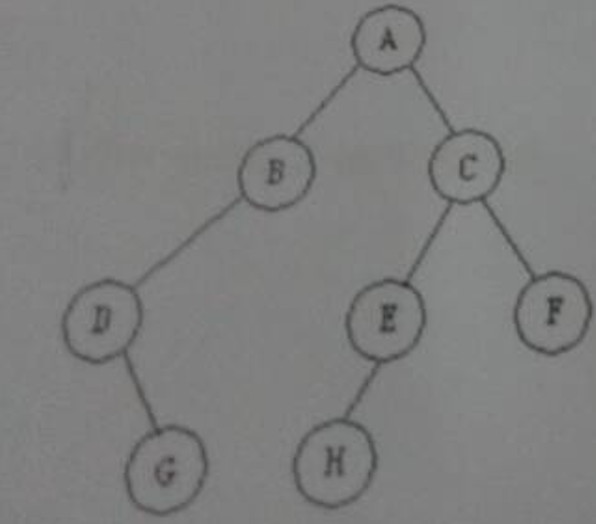
\includegraphics[width=.9\linewidth]{./pic/tree.png}
\end{center}
\item 写出一个C类ip地址(192.168.1.105),该ip地址一个合法的网格掩码是(255.255.255.224).
\item c/c++程序运行时有堆内存与栈内存之分,请写一个语句在堆中分配一个整数:(int a = new int(4)),在栈内存中分配一个整数:(int a = 5)。
\item 简述从C/C++源代码生成可执行文件所经历的几个过程和每个过程中所做的事情。
\end{itemize}
预编译-》编译-》链接-》执行
\begin{itemize}
\item 简述TCP建立连接的过程,最好能画出时序图。
\begin{itemize}
\item 三次握手;
\end{itemize}
\item 有一个c语言函数
\begin{minted}[linenos=true]{java}
unsigned int getN(unsigned int v){
    v--;
    v |= v >> 1;
    v |= v >> 2;
    v |= v >> 4;
    v |= v >> 8;
    v |= v >> 16;
    v++;
    return v;
}
\end{minted}
\end{itemize}

请问这个函数的功能是什么?
\begin{itemize}
\item 返回的结果是v 或者 2 \^{} 跟下v次方 + 1(比如125返回128,128返回的就是128)
\end{itemize}
\begin{itemize}
\item 列出c语言中static关键字的用法。
\begin{itemize}
\item static 关键字至少有下列几个作用:
\begin{itemize}
\item (1)函数体内static 变量的作用范围为该函数体,不同于auto 变量,该变量的内存只被分配一次,因此其值在下次调用时仍维持上次的值;
\item (2)在模块内的static 全局变量可以被模块内所用函数访问,但不能被模块外其它函数访问;
\item (3)在模块内的static 函数只可被这一模块内的其它函数调用,这个函数的使用范围被限制在声明它的模块内;
\item (4)在类中的static 成员变量属于整个类所拥有,对类的所有对象只有一份拷贝;
\item (5)在类中的static 成员函数属于整个类所拥有,这个函数不接收this 指针,因而只能访问类的static 成员变量。
\end{itemize}
\end{itemize}
\item 解释一下Unity3D中的协程(coroutine)是什么?并举例说明
\begin{itemize}
\item 在主线程运行的同时开启另一段逻辑处理,来协助当前程序的执行,协程很像多线程,但是不是多线程,Unity的协程实在每帧结束之后去检测yield的条件是否满足。
\end{itemize}
\item 物体自旋转使用的函数叫什么?物体绕某点旋转使用函数叫什么?
\begin{itemize}
\item 物体自旋转函数transform.Rotate,物体绕某点旋转函数:transform.RotateAround
\end{itemize}
\item 使用prefab预制物体有什么好处?
\begin{itemize}
\item 1.Prefab一个重要的优势就是编辑prefab资源后,场景中所有使用Prefab克隆的游戏对象将全部使用新编辑的资源,无需一个一个的给场景中的对象赋值。
\item 2.当游戏中需要频繁创建一个物体时,使用Prefab能够节省内存。
\item 3.当你在一个场景中增加一个Prefabs,你就实例化了一个Prefabs。
\end{itemize}
\item 设有如下关系表R1和R2
\begin{itemize}
\item R1(NO, NAME, SEX, AGE, CLASS)
\item R2(NO, SUBJECT, SCORE)
\item 主关键字是NO,其中NO为学号,NAME为姓名,SEX为性别,AGE为年龄,CLASS为班号,SUBJECT为科目,SCORE为成绩。写出实现下列功能的SQL语句。查找学号为20的学生的姓名,科目,成绩。
\item SELECT NAME,SUBJECT,SCORE FORM R1 INNER JOIN R2 ON R1.NO=R2.NO WHERE R1.NO = 20
\end{itemize}
\item 描述多人联网中位置的同步和聊天通讯的实现方法,并编程写出如何实现多人协同中交互操作。(交互操作例如,血值为100的两个角色人物可以相互射击双方,射击一次减去血值10,当血值为0的时候证明已经死亡)
\item 当实例化一个prefab对象,prefab对象上面挂载了一个继承MonoBehaviour的脚本
\begin{itemize}
\item 1.请问这个脚本分别会按顺序调用哪些函数,并列出哪些函数是反复进去的
\item 2.请问当这个实例化对象先调用了SetActive(false),然后又调用了SetActive(true),那么这个脚本依次会调用哪些函数方法?
\item 3.如果在脚本的Awake()函数中,调用了this.gameObject.AddComponent()(PS:GameController为另一个继承Mono的脚本类),请问此时脚本函数的调用顺序是否发生变化?
\end{itemize}
\item if(go.CompareTag(“Enemy”))和if(go.tag == “Enemy”)两种判断方法哪种是合适的,为什么?
\begin{itemize}
\item 第一种合适,因为第二种会占用更多内存。
\end{itemize}
\item DestroyImmediate和Destroy的区别是?
\begin{itemize}
\item DestroyImmeditate 销毁对象的时候,会立即释放资源。Destroy只是从该场景销毁,但是还在内存当中。
\end{itemize}
\item 详细说明Unity中资源加载的方法,以及他们的区别?
\begin{itemize}
\item 1.通过Resources模块,调用它的load函数:可以直接load并返回某个类型的Object,前提是要把这个资源放在Resource命名的文件夹下,Unity不关有没有场景引用,都会将其全部打入到安装包中。
\item 2.通过bundle的形式:即将资源打成 asset bundle 放在服务器或本地磁盘,然后使用WWW模块get 下来,然后从这个bundle中load某个object。
\end{itemize}
\item 从代码角度上如何进行内存优化?
\item 分别写出Invoke和协程的几种用法?
\item 以下函数的功能是计算斐波那契数列的第n项,请填空
\begin{minted}[linenos=true]{java}
int func(int n) {
    if(n<=2) return 1;
    return n + func(n-1);
}
\end{minted}
\item C语言中宏定义中若有多行,可以使用字符($\backslash$).
\item C语言中32位整数能表达的最小的数是-2\textsuperscript{31}\textasciitilde{}2\textsuperscript{31}-1.
\item 使用(点乘)向量运算可以很方便地计算出三维空间中两个单位向量之间夹角的cos值。
\item 类unix系统中某文件的权限为:drw-r–r–,用八进制数值形式表示该权限为(411),首位d代表目录(文件夹)
\item 若有如下程序段,其中s,a,b,c均已定义为整型变量,且a,c均已赋值(c大于0)
\begin{minted}[linenos=true]{java}
s = a;
for(b = 1; b <= c; b++)
    s = s + 1;
\end{minted}
\end{itemize}

则与上述程序段功能等价的赋值语句是(B)
\begin{itemize}
\item A.s = a + b
\item B.s = a + c
\item C.s = s + c
\item D.s = b + c
\end{itemize}
\begin{itemize}
\item 简述static和const关键字的作用
\begin{itemize}
\item static 关键字至少有下列几个作用:
\begin{itemize}
\item (1)函数体内static 变量的作用范围为该函数体,不同于auto 变量,该变量的内存只被分配一次,因此其值在下次调用时仍维持上次的值;
\item (2)在模块内的static 全局变量可以被模块内所用函数访问,但不能被模块外其它函数访问;
\item (3)在模块内的static 函数只可被这一模块内的其它函数调用,这个函数的使用范围被限制在声明它的模块内;
\item (4)在类中的static 成员变量属于整个类所拥有,对类的所有对象只有一份拷贝;
\item (5)在类中的static 成员函数属于整个类所拥有,这个函数不接收this 指针,因而只能访问类的static 成员变量。
\end{itemize}
\item const 关键字至少有下列几个作用:
\begin{itemize}
\item (1)欲阻止一个变量被改变,可以使用const 关键字。在定义该const 变量时,通常需要对它进行初始化,因为以后就没有机会再去改变它了;
\item (2)对指针来说,可以指定指针本身为const,也可以指定指针所指的数据为const,或二者同时指定为const;
\item (3)在一个函数声明中,const 可以修饰形参,表明它是一个输入参数,在函数内部不能改变其值;
\item (4)对于类的成员函数,若指定其为const 类型,则表明其是一个常函数,不能修改类的成员变量;
\item (5)对于类的成员函数,有时候必须指定其返回值为const 类型,以使得其返回值不为“左值”。
\end{itemize}
\end{itemize}
\item 用你熟悉的语言及你认为最简洁的方法书写计算 s = 1!+2!+3!+…+num!的代码。num为输入,s为输出。(!代表阶乘 3!= 1 * 2 * 3
\begin{minted}[linenos=true]{java}
Console.ReadLine(num)
int s = 0;
for(int i = 1; i <= num; i++) {
    s += JieCheng(num);
}
public int JieCheng(int num) {
    if(num < 0) {
        Console.WriteLine("error");
        return;
    }
    if(num <=1) {
        return 1;
    } else {
        return num * JieCheng(num - 1)
            }
}
\end{minted}
\item 用你熟悉的语言从一个字符串中去掉相连的重复字符,例如原字符串“adffjkljaalkjhl”变为“adfjkljalkjhl”
\begin{minted}[linenos=true]{java}
int GetResult(char[] input, char[] output)   {  
    int i, j, k = 0;  
    int flag;  
    int length;  
    if(input == NULL || output == NULL)   {  
        return -1;  
    }  
    length=strlen(input);//求数组的长度  
    for(i = 0; i<length; i++)   {  
        flag = 1;  
        for(j = 0; j < i; j++)   {  
            if(output[j] == input [i])  
                flag = 0;  
        }  
        if(flag)  
            output[k++] = input[i];  
    }  
    printf("最终的字符串为:");  
    output[k] = '\0';  
    for(int m = 0; m < output.Length; m++) {
        print (output [m]);
    } 
    return 0;  
}  
\end{minted}
\end{itemize}

\section{第二部分}
\label{sec:org01e7247}
\begin{itemize}
\item 哪种实时光源是Unity中没有的?(D)
\begin{itemize}
\item A.点光源
\item B.方向光
\item C.聚光灯
\item D.日光灯
\end{itemize}
\item 如何在Unity中创建地形系统?(D)
\begin{itemize}
\item A.Terrain->Create Terrain
\item B.Component->Create Terrain
\item C.Asset->Create Terrain
\item D.Windows->Create Terrain
\end{itemize}
\item 以下哪种操作步骤可以在场景中添加“Wind Zone”?(B)
\begin{itemize}
\item A.Terrain->Wind Zone
\item B.GameObject->Create other->Wind Zone
\item C.Component->Physics->Wind Zone
\item D.Assets->Create->Wind Zone
\end{itemize}
\item 在Unity编辑器中创建一个Directional Light,以下步骤正确的是?(B)
\begin{itemize}
\item A.Edit->Rendering Setting->Directional Light
\item B.GameObject->Create Other->Directional Light
\item C.Component->Rendering->Directional Light
\item D.Assets->Directional Light
\end{itemize}
\item 下列哪一项不属于Camera中的“Clear Flags”?(D)
\begin{itemize}
\item A.Skybox
\item B.Solid Color
\item C.Depth Only
\item D.Background
\end{itemize}
\item 以下哪种脚本语言是Unity编辑器所不支持的?(D)
\begin{itemize}
\item A.Javascript
\item B.C\#
\item C.Boo
\item D.Perl
\end{itemize}
\item 对于Prefab,以下说法错误的是?(D)
\begin{itemize}
\item A.Prefab资源可以在项目中多次重复使用
\item B.由Prefab实例出的GameObject,其在Hierarchy试图中表现为蓝色
\item C.Prefab上的组件信息一经改变,其实例出的GameObject也会自动改变
\item D.实例出的GameObject上的组件信息一经改变,其对应出的Prefab也会自动改变
\end{itemize}
\item 下面哪种做法可以打开Unity的Asset Store?(A)
\begin{itemize}
\item A.Windows->Asset Store
\item B.Edit->Asset Store
\item C.File->Asset Store
\item D.Assets->Asset Store
\end{itemize}
\item 在哪个面板中可以修改物体的空间属性,如位置,朝向,大小等(B)
\begin{itemize}
\item A.Project
\item B.Inspector
\item C.Hierarchy
\item D.Toolbar
\end{itemize}
\item 如何为一个Asset 资源设定一个Label,从而能够方便准确的搜索到?(D)
\begin{itemize}
\item A.在Project窗口中选中一个Asset,右键->Create->Label
\item B.在Project窗口中选中一个Asset,右键->Add Label
\item C.在Project窗口中选中一个Asset,在Inspector窗口中点击添加Label的图标
\item D.在Project窗口中选中一个Asset,在Inspector窗口中点击按钮“Add Label”
\end{itemize}
\item Mecanim系统中,Body Mask的作用是?(D)
\begin{itemize}
\item A.指定身体的某一部分是否参与骨骼动画
\item B.指定身体的某一部分是否参与物理模拟
\item C.指定身体的某一部分是否可以输出骨骼信息
\item D.指定身体的某一部分是否参与渲染
\end{itemize}
\item 以下哪种操作步骤可以打开Unity编辑器的Lightmapping视图?(C)
\begin{itemize}
\item A.File->Lightmapping
\item B.Assets->Lightmapping
\item C.Windows->Lightmapping
\item D.Component->Lightmapping
\end{itemize}
\item 下列关于光照贴图,说法错误的是?(C)
\begin{itemize}
\item A.使用光照贴图比使用实时光源渲染要快
\item B.可以降低游戏内存消耗
\item C.可以增加场景真实感
\item D.多个物体可以使用同一张光照贴图
\end{itemize}
\item 如何为物体添加光照贴图所使用的UV?(B)
\begin{itemize}
\item A.不用添加,任何时候都会自动生成
\item B.更改物体导入设置,勾选“Generate Lighting UVs”
\item C.更改物体导入设置,勾选“Swap UVs”
\item D.更改物体导入设置,在UVs选项中选择“Use Lightmaps”
\end{itemize}
\item 在哪个模块下可以修改Render Path?(A)
\begin{itemize}
\item A.Camera
\item B.Light
\item C.Render Settings
\item D.Project Setting->Quality
\end{itemize}
\item 以下哪项技术下不是目前Unity所支持的Occlusion Culling技术?(D)
\begin{itemize}
\item A.PVS only
\item B.PVS and dynamic objets
\item C.Automatic Portal Generation
\item D.Dynamic Only
\end{itemize}
\item 关于Vector3的API,以下说法正确的是?(C)
\begin{itemize}
\item A.Vector3.normalize可以获取一个三维向量的法线向量
\item B.Vector3.magnitude可以获取一个三维向量的长度
\item C.Vector3.forward与Vector3(0,0,1)是一样的
\item D.Vector3.Dot(向量A,向量B)是用来计算向量A与向量B的叉乘
\end{itemize}
\item 下列那些选项不是网格层属性的固有选项?(B)
\begin{itemize}
\item A.Default
\item B.Walkable
\item C.Not Walkable
\item D.Jump
\end{itemize}
\item 写出你对游戏的理解及游戏在生活中的作用,对Unity3D软件理解最深入的地方。
\end{itemize}

\section{C++}
\label{sec:orgd8b7854}
\begin{itemize}
\item 请写代码打印100之内的素数,讲求效率(请做你的解法的效率分析)
\item 求m,n的最大公约数
\item 输入10个字符串,打印出其中重复的字符串以及重复的次数
\item 请画图例(UML最好),给出windows下的文件目录的设计模式
\item 用OO表示狼吃羊羊吃草
\item 什么是subversion?它与vss,cvs的区别在哪?或者有什么优势?
\item 什么是wiki,关于程序项目的wiki你使用过哪些?wiki对你有什么帮助吗?wiki与程序文挡的差别在哪?
\item 什么是tdd?你使用过吗?tdd的关键在哪?跟传统的单元测试相比,有什么优越性?
\item 什么是单元测试?你用过哪些单元测试工具?他们的区别和好处各有哪些?你主要倾向于哪一种?
\item 什么是编程规范?你倾向于什么样的规范?他的好处在哪?
\item 什么是mfc?你经常使用那些mfc类?那么为什么很多人不主张使用mfc?
\item 什么是头文件依赖?你注意过这些问题吗?你注意过编译的时间吗?你怎么改进编译时间?
\item 什么是面向对象?你在哪些方面用过面向对象?带来了什么好处?又有什么弊端?
\item 什么是接口编程.com,他带来了什么好处?适用于什么地方?
\item 什么是设计模式?使用设计模式有什么好处?列举你使用过的设计模式知识:
\item 一寸山河一寸血,\_\_\_\_\_\_\_\_\_\_\_。是\_\_\_\_\textsubscript{说的}。
\item 抗战历时\_\_\_\textsubscript{年},最多百分之\_\_\_\textsubscript{的土地沦陷},军民伤亡\_\_\_\_。
\end{itemize}
\end{document}